%\documentclass{bxjsarticle}
%\documentclass[]{article}
\documentclass[openany]{book}

\usepackage{zxjatype}
\usepackage[ipa]{zxjafont}
\usepackage[overlap,CJK]{ruby} %添加这个增加对于日文拼音的支持

\setlength\paperheight{210mm}
\setlength\paperwidth{148mm}

\usepackage{geometry}
\geometry{left=1cm,right=1cm,top=2cm,bottom=2cm}

\usepackage{setspace} %添加这个用于行距修改
\usepackage{verbatim}%用于多行注释
\usepackage{color}
\usepackage[bookmarks=true,colorlinks,linkcolor=black]{hyperref}
\usepackage{lipsum}
\usepackage{fancyhdr}
\usepackage{graphicx}%封面相关
\usepackage[english]{babel}
\usepackage{blindtext}
\usepackage{pst-node,graphicx}
\SpecialCoor

\usepackage{picins}

\usepackage{hyperref}

\begin{document}

\noindent\pnode(0.5\textwidth,-0.5\textheight){Center}
\rput(Center){
\includegraphics[width=\paperwidth]{1.eps}}

\setcounter{page}{0}

%% temporary titles
% command to provide stretchy vertical space in proportion
\newcommand\nbvspace[1][3]{\vspace*{\stretch{#1}}}
% allow some slack to avoid under/overfull boxes
\newcommand\nbstretchyspace{\spaceskip0.5em plus 0.25em minus 0.25em}
% To improve spacing on titlepages
\newcommand{\nbtitlestretch}{\spaceskip0.6em}
\pagestyle{empty}
\begin{center}
\bfseries
\nbvspace[1]
\Huge
{\nbtitlestretch\huge
AWK ONE LINERS EXPLAINED}

\nbvspace[1]
\normalsize

TO WHICH IS ADDED MANY USEFUL ONE\\
LINERS AND CODE SO THAT\\
YOU CAN AWK LIKE A HAWK
\nbvspace[1]
\small BY\\
\Large PETERIS KRUMINS\\[0.5em]
\footnotesize AUTHOR OF ``A WORKING ALGEBRA,'' ``WIRELESS TELEGRAPHY,\\
ITS HISTORY, THEORY AND PRACTICE,'' ETC., ETC.
\nbvspace[2]

%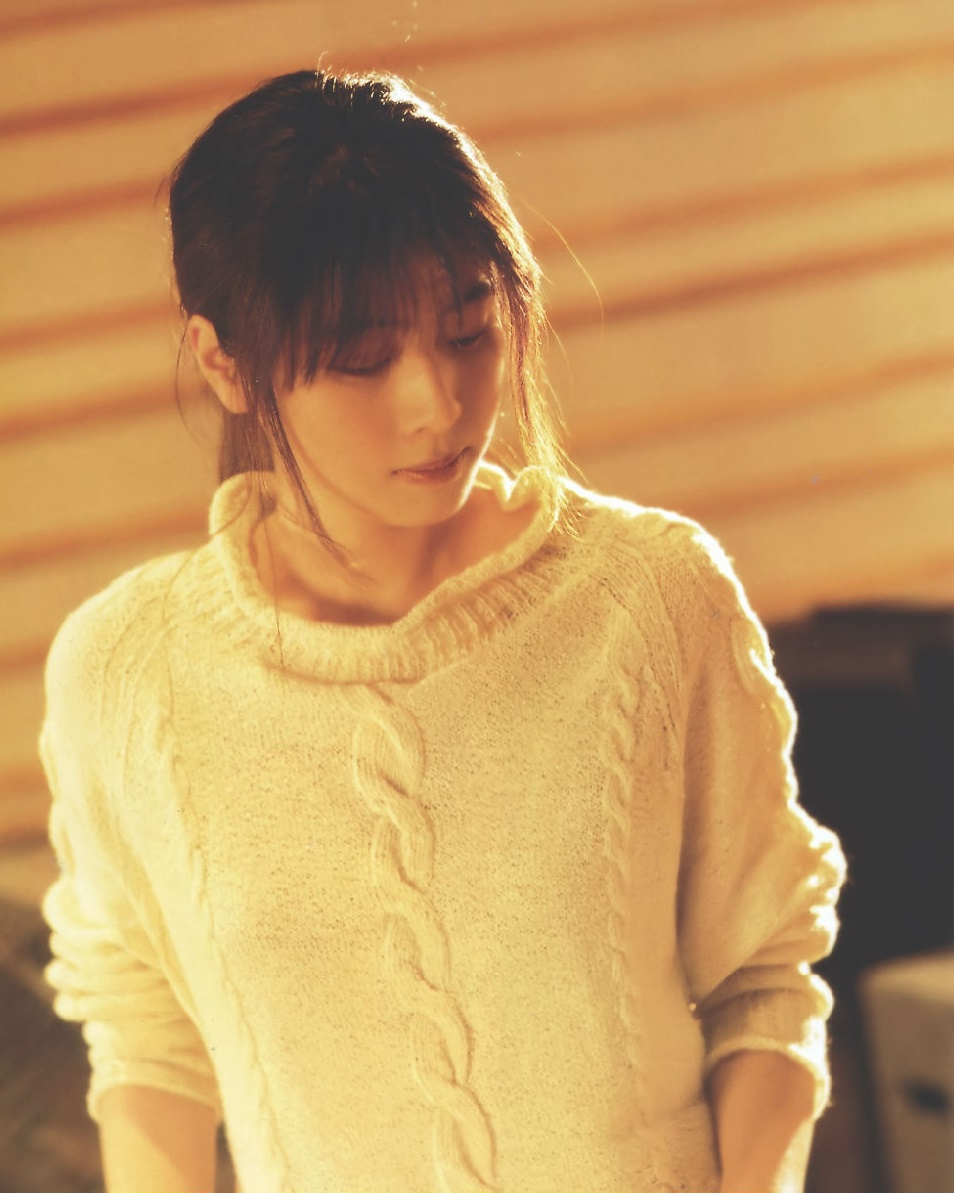
\includegraphics[width=1.5in]{bkg.jpg}
\nbvspace[3]
\normalsize

DOHA\\
\large
PUBLISHED IN THE WILD
\nbvspace[1]
\end{center}

\thispagestyle{empty} %本页頁碼空白




\pagestyle{fancy}                    % 设置页眉
%\rhead{\small\leftmark}
%===============
%双线页眉的设置
\makeatletter %双线页眉
\def\headrule{{\if@fancyplain\let\headrulewidth\plainheadrulewidth\fi%
%\hrule\@height 1.0pt \@width\headwidth\vskip1pt%上面线为1pt粗
\hrule\@height 0.5pt\@width\headwidth  %下面0.5pt粗
\vskip-2\headrulewidth\vskip-1pt}      %两条线的距离1pt
  \vspace{6mm}}     %双线与下面正文之间的垂直间距
\makeatother
%===============

\begin{spacing}{1.3}

\thispagestyle{empty} %本页頁碼空白
\tableofcontents

\vspace{-10mm}


\chapter{Album 1}
\thispagestyle{empty} %本页頁碼空白
\vspace{-16mm}
\LARGE {Good-bye My Loneliness}

\normalsize{BGCH-1003 1991.3.27 \ release}
\\

\vspace{-5mm}

\parpic[l]{
\pichskip{6em}
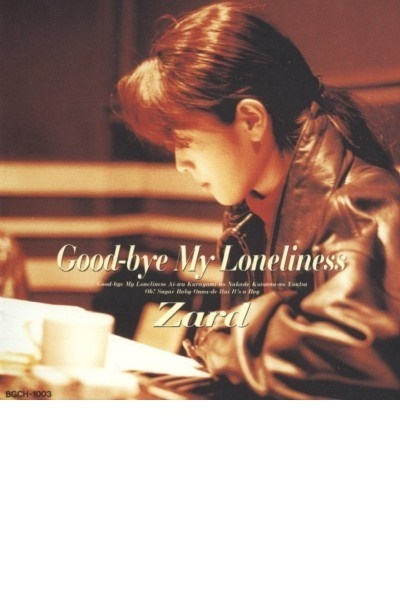
\includegraphics[width=0.4\textwidth]{1.jpg}}

\small{\hyperlink{1_0}{1.Good-bye My Loneliness}}

\tiny{作詞:坂井泉水 \ 作曲:織田哲郎 \ 編曲:明石昌夫}

\small{\hyperlink{1_1}{2.愛は暗闇の中で}}

\tiny{作詞:坂井泉水 \ 作曲:栗林誠一郎 \ 編曲:ZARD/寺尾広}

\small{\hyperlink{1_2}{3.恋女の憂鬱 }}

\tiny{作詞/作曲:川島だりあ \ 編曲:明石昌夫}

\small{\hyperlink{1_3}{4.Oh! Sugar Baby}}

\tiny{作詞:坂井泉水 \ 作曲:栗林誠一郎 \ 編曲:葉山たけし}

\small{\hyperlink{1_4}{5.女でいたい }}

\tiny{作詞/作曲:川島だりあ \ 編曲:葉山たけし}

\small{\hyperlink{1_5}{6.It's a Boy}}

\tiny{作詞:坂井泉水 \ 作曲:栗林誠一郎 \ 編曲:明石昌夫}

\small{ \ }

\tiny{ \ }

\small{ \ }

\tiny{ \ }

\small{ \ }

\tiny{ \ }

\small{ \ }

\tiny{ \ }

\small{ \ }

\tiny{ \ }

\small{ \ }

\tiny{ \ }

\clearpage


\hypertarget{1_0}{}
\section{ Good-bye My Loneliness}

\parpic[r]{
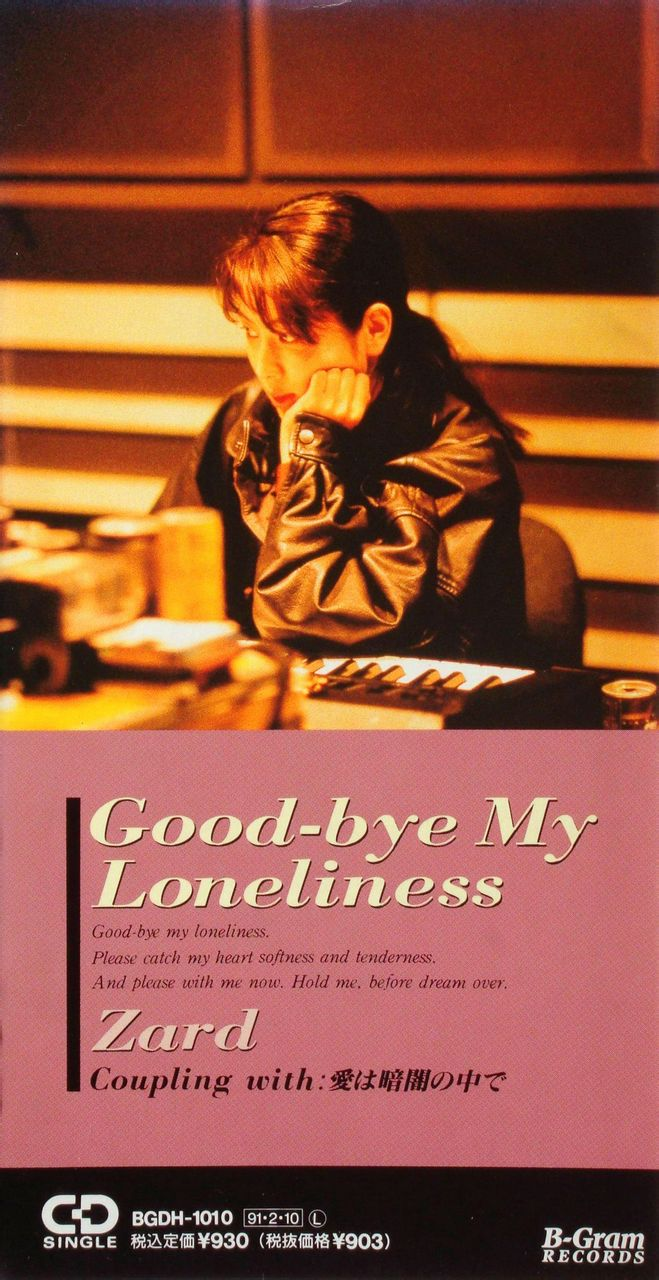
\includegraphics[width=0.3\textwidth]{S1.jpg}}

\large{

\ruby{心}{こころ}の\ruby{奥}{おく}を あなたに のぞかれそう

\ruby{瞳}{め}をそらしても \ruby{気}{き}づかれそうで

\ruby{煙}{けむ}る\ruby{都会}{とかい}の Rain drops

\ruby{揺}{ゆ}らいでいたの

また\ruby{独}{ひと}りに なるのが\ruby{怖}{こわ}くて
\\

Good-bye my loneliness

あなたの\ruby{胸}{むね}に そっと Tenderness

\ruby{飛}{と}び\ruby{込}{こ}みたいの

だから\ruby{今}{いま}は そばにいて\ruby{欲}{ほ}しいの

\ruby{抱}{だ}きしめて \ruby{夢}{ゆめ}が\ruby{消}{き}える\ruby{前}{まえ}に
\\

つれない\ruby{恋}{こい}の \ruby{行方}{ゆくえ}は \ruby{季節}{きせつ}まかせ

いつも\ruby{未来}{みらい}が \ruby{雨}{あめ}でみえない

\ruby{霞}{かす}む\ruby{都会}{とかい}の Tear drops

\ruby{臆病}{おくびゅう}になるの

さめた\ruby{想}{おも}い あたためて\ruby{欲}{ほ}しい
\\

Good-bye my loneliness

\ruby{信}{しん}じていても ふたり Faraway

\ruby{思}{おも}い\ruby{出}{で}になる

だから\ruby{今}{いま}は そばにいて\ruby{欲}{ほ}しいの

\ruby{抱}{だ}きしめて すべて \ruby{忘}{わす}れさせて
\\

Good-bye my loneliness

\ruby{信}{しん}じていても きっと Faraway

\ruby{思}{おも}い\ruby{出}{で}になる

だから\ruby{今}{いま}は \ruby{行}{い}かないで\ruby{欲}{ほ}しいの

\ruby{抱}{だ}きしめて \ruby{夢}{ゆめ}が\ruby{消}{き}える\ruby{前}{まえ}に

}

\hypertarget{1_1}{}
\section{ 愛は暗闇の中で}
\large{

\ruby{愛}{あい}は\ruby{手探}{てさぐ}り

\ruby{暗闇}{くらやみ}の\ruby{中}{なか}で

\ruby{踊}{おど}る It's gonna be a great night, yeah~
\\

\ruby{駆}{か}け\ruby{拔}{ぬ}ける Freeway

この\ruby{思}{おも}い To be your slave

Oh, you, crazy rainy night, no one care

\ruby{素直}{すなお}になれ Night \ruby{濡}{ぬ}れた Memories
\\

こんなにも For you

\ruby{感}{かん}じてる But you're so cold

Oh! Tonight and everynight, you'd be mine

\ruby{目移}{めうつ}り\ruby{気}{き}になる

\ruby{恋}{こい}の\ruby{駆}{か}け\ruby{引}{ひ}き
\\

\ruby{愛}{あい}は\ruby{手探}{てさぐ}り

\ruby{暗闇}{くらやみ}の\ruby{中}{なか}で

\ruby{踊}{おど}る It's gonna be a great night, yeah~

\ruby{愛}{あい}は\ruby{気}{き}まぐれ \ruby{Beat}{ビート}に\ruby{抱}{だ}かれ

\ruby{見}{み}つめて In your eyes. oh yeah~
\\

\ruby{夜明}{よあ}けの Highway

つぶやいた To change your mind

Oh, crazy crazy night, no one care

\ruby{甘}{あま}く\ruby{切}{せつ}ない\ruby{心}{こころ}に In my dream
\\

\ruby{愛}{あい}はまぼろし\ruby{暗闇}{くらやみ}の\ruby{中}{なか}で

\ruby{踊}{おど}る It's gonna be a great night, yeah~

\ruby{愛}{あい}は\ruby{震}{ふる}えて \ruby{Beat}{ビート}に\ruby{抱}{だ}かれ

このまま In your eyes. oh yeah
\\

\ruby{愛}{あい}は\ruby{手探}{てさぐ}り

\ruby{暗闇}{くらやみ}の\ruby{中}{なか}で

\ruby{踊}{おど}る It's gonna be a great night, yeah~

\ruby{愛}{あい}は\ruby{気}{き}まぐれ \ruby{Beat}{ビート}に\ruby{抱}{だ}かれ

\ruby{見}{み}つめて In your eyes
\\

\ruby{愛}{あい}は\ruby{手探}{てさぐ}り

\ruby{暗闇}{くらやみ}の\ruby{中}{なか}で

\ruby{踊}{おど}る It's gonna be a great night, yeah~

\ruby{愛}{あい}は\ruby{震}{ふる}えて \ruby{Beat}{ビート}に\ruby{抱}{だ}かれ

このまま In your eyes. oh yeah
\\

}

\hypertarget{1_2}{}
\section{ 恋女の憂鬱}
\large{

\ruby{声}{こえ}が\ruby{聞}{き}きたい

\ruby{誰}{だれ}といるの?

\ruby{今}{いま}どこにいるの?

\ruby{音}{おと}のでてない

\ruby{テレビ}{television} \ruby{ドラマ}{drama}

つめをかんで\ruby{見}{み}てる

\ruby{愛}{あい}する\ruby{男}{ひと}がいると

\ruby{優}{やさ}しくなれない

\ruby{笑顔}{えがお}のなか\ruby{噓}{うそ}を\ruby{探}{さが}してる
\\

\ruby{恋}{こい}\ruby{女}{おんな}の\ruby{憂鬱}{ゆうう}つがおどる

サヨナラが\ruby{怖}{こわ}いよと

\ruby{永遠}{えいえん}に\ruby{眠}{ねむ}らない

\ruby{痛}{いた}みならば\ruby{艶}{あで}やかに
\\

\ruby{明日}{あした}でもない

\ruby{今度}{こんど}でもない

\ruby{今}{いま}すぐ\ruby{会}{あ}いたい

わがままを

したい\ruby{時}{とき}に

あなたはいないね

\ruby{軽}{かる}く\ruby{閉}{と}じたまつ\ruby{毛}{げ}

\ruby{鏡}{かがみ}のおくで

やり\ruby{場}{ば}もなくふるえてる
\\

\ruby{恋}{こい}\ruby{女}{おんな}の\ruby{憂鬱}{ゆうう}つがおどる

サヨナラが\ruby{怖}{こわ}いよと

\ruby{永遠}{えいえん}に\ruby{眠}{ねむ}らない

\ruby{痛}{いた}みならば\ruby{艶}{あで}やかに
\\

\ruby{恋}{こい} \ruby{女}{おんな}のゆううつがおどる

サヨナラが\ruby{怖}{こわ}いよと

\ruby{永遠}{えいえん}に\ruby{眠}{ねむ}らない

\ruby{痛}{いた}みならば\ruby{艶}{あで}やかに

}

\hypertarget{1_3}{}
\section{ Oh! Sugar Baby}
\large{

Everybody ねぇ \ruby{聞}{き}いてよ

\ruby{ロングヘア}{long hair}をなびかせて

はやるの\ruby{服}{ふく}を\ruby{着}{き}こなして

\ruby{自慢}{じまん}の\ruby{レッグ}{leg}で sexy walk

うわさはいろいろあるよ

でも\ruby{誰}{だれ}もが\ruby{君}{きみ}に\ruby{夢中}{むちゅう}だよ
\\

Oh, sugar baby \ruby{君}{きみ}に\ruby{恋}{こい}したよ

\ruby{少}{すこ}しは\ruby{僕}{ぼく}を\ruby{意識}{いしき}してほしい
\\

Everybody ねぇ \ruby{聞}{き}いてよ

\ruby{彼女}{かのじょ}がこう\ruby{言}{い}うんだ

“\ruby{真面目}{まじめ}なのもいいけと\ruby{悪}{わる}い\ruby{男}{おとこ}も\ruby{素敵}{すてき}”

\ruby{見}{み}かけだけじゃないよ

\ruby{男}{おとこ}は\ruby{ハート}{heart}で\ruby{決}{き}まるよ
\\

Oh, sugar baby \ruby{君}{きみ}に\ruby{恋}{こい}してるよ

\ruby{少}{すこ}しは\ruby{僕}{ぼく}を\ruby{意識}{いしき}してほしい
\\

Everybody ねぇ \ruby{聞}{き}いてよ

\ruby{彼女}{かのじょ}がこう\ruby{言}{い}うんだ

“Kissが\ruby{輕}{かる}すぎるわ\ruby{。最近}{さいきん}\ruby{冷}{つめ}たいのね”

\ruby{遊}{あそ}びなんかじゃないよ

すこし\ruby{退屈}{たいくつ}なだけだよ
\\

Oh, sugar baby \ruby{君}{きみ}に\ruby{恋}{こい}してるよ

Oh, sugar baby \ruby{君}{きみ}に\ruby{恋}{こい}してるよ
\\

Sugar sugar baby \ruby{君}{きみ}に\ruby{恋}{こい}してるよ

\ruby{少}{すこ}しは\ruby{僕}{ぼく}を\ruby{意識}{いしき}してほしい
\\

Oh, sugar baby \ruby{君}{きみ}に\ruby{恋}{こい}してるよ

Oh, sugar baby \ruby{君}{きみ}に\ruby{恋}{こい}してるよ
\\

Sugar sugar baby \ruby{君}{きみ}に\ruby{恋}{こい}してるよ

\ruby{少}{すこ}しは\ruby{僕}{ぼく}を\ruby{意識}{いしき}してほしい

}

\hypertarget{1_4}{}
\section{ 女でいたい}
\large{

12\ruby{月}{がつ}の\ruby{夏}{なつ}

\ruby{見知}{みし}らぬ\ruby{アパート}{apartment house}

\ruby{素足}{すあし}の\ruby{ヒール}{heel}をそっと\ruby{外}{はず}した

あいつを\ruby{愛}{あい}して

あまりに\ruby{近}{ちか}くて

\ruby{嫌}{きら}いになるのは\ruby{簡単}{かんたん}だった
\\

\ruby{疲}{つか}れた\ruby{肌}{はだ}

\ruby{南}{みなみ}に\ruby{徴発}{ちょうはつ}された\ruby{恋}{こい}

\ruby{名前}{なまえ}は\ruby{聞}{き}かない

\ruby{女}{おんな}でいたい
\\

Keep on love tonight,

I'll never fallin' in love

\ruby{泣}{な}き\ruby{顔}{がお}に\ruby{愛}{あい} \ruby{探}{さが}さないで

もう\ruby{一度}{いちど}あいつのもとへ

\ruby{変}{か}えれぬ\ruby{勇気}{ゆうき}がほしいだけ
\\

\ruby{二人}{ふたり}の\ruby{出逢}{であ}った

あの\ruby{頃}{ころ}のように

\ruby{不安}{ふあん}の\ruby{海}{うみ}を\ruby{泳}{およ}いでいたい

\ruby{体}{からだ}を\ruby{重}{かさ}ねても

くちずけをしない

\ruby{馴}{な}れすぎた\ruby{夜}{よる}に

\ruby{何}{なに}を\ruby{飾}{かざ}ろう
\\

\ruby{優}{やさ}しさは

\ruby{時}{とき}に\ruby{人}{ひと}を\ruby{噓}{うそ}つきにする

ためらいもなく
\\

\ruby{女}{おんな}でいたい

Keep on love tonight,

I'll never fallin' in love

だかれて\ruby{委}{ゆだ}ねる\ruby{冬}{ふゆ}の\ruby{心}{こころ}

\ruby{愛}{いと}しいあいつがよぎれば

\ruby{瞼}{まぶた}に\ruby{涙}{なみだ}の\ruby{意味}{いみ}を\ruby{知}{し}る
\\

Keep on love tonight,

I'll never fallin' in love

\ruby{泣}{な}き\ruby{顔}{がお}に\ruby{愛}{あい} \ruby{探}{さが}さないで

もう\ruby{一度}{いちど}あいつのもとへ

\ruby{変}{か}えれぬ\ruby{勇気}{ゆうき}がほしいだけ
\\

Keep on love tonight,

I'll never fallin' in love

だかれて\ruby{委}{ゆだ}ねる\ruby{冬}{ふゆ}の\ruby{心}{こころ}

\ruby{愛}{あい}しいあいつがよぎれば

\ruby{瞼}{まぶた}に\ruby{涙}{なみだ}の\ruby{意味}{いみ}を\ruby{知}{し}る

}

\hypertarget{1_5}{}
\section{ It's a Boy}
\large{

\ruby{年}{とし}が\ruby{離}{はな}れていても

\ruby{気}{き}が\ruby{弱}{よわ}くても

\ruby{大丈夫}{だいじょうぶ} \ruby{気}{き}にしないで

\ruby{愛}{あい}がゆらいでいたら

すぐ\ruby{分}{わ}かるから

こう\ruby{見}{み}えても\ruby{意外}{いがい}と\ruby{強}{つよ}いから
\\

Oh いつまでも\ruby{変}{か}わらないで Boy

Ah \ruby{優}{やさ}しさで\ruby{包}{つつ}んであげる 
\\

こんなにも loving you \ruby{目}{め}を\ruby{閉}{と}じて

So day & night hold me tight all the night

It's a boy oh…

mm…… Hold me tight all the night

It's a boy
\\

\ruby{朝}{あさ}もや\ruby{光}{ひかり}のなか

\ruby{君}{きみ}はまだ\ruby{夢}{ゆめ}のなか

\ruby{二人}{ふたり}のことまだ\ruby{知}{し}らない\ruby{誰}{だれ}も
\\

Oh いつまでも\ruby{見}{み}つからないで Boy

Ah \ruby{気}{き}づかれずそっと\ruby{痛}{いた}いから
\\

こんなにも loving you \ruby{抱}{だ}きしめて Boy

So day & night all the day all the night

こんなにも loving you \ruby{覚}{さ}めるまで

So day & night hold me tight all the night

It's a boy

}


\chapter{Album 2}
\thispagestyle{empty} %本页頁碼空白
\vspace{-16mm}
\LARGE {もう探さない}

\normalsize{BGCH-1004 1991.12.25 \ release}
\\

\vspace{-5mm}

\parpic[l]{
\pichskip{6em}
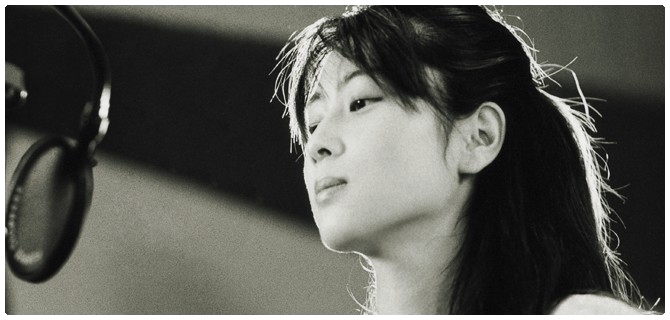
\includegraphics[width=0.4\textwidth]{2.jpg}}

\small{\hyperlink{2_0}{1.不思議ね…}}

\tiny{作詞:坂井泉水 \ 作曲:織田哲郎 \ 編曲:明石昌夫}

\small{\hyperlink{2_1}{2.もう探さない}}

\tiny{作詞:坂井泉水 \ 作曲:織田哲郎 \ 編曲:明石昌夫}

\small{\hyperlink{2_2}{3.素直に言えなくて}}

\tiny{作詞/作曲:坂井泉水 \ 編曲:明石昌夫}

\small{\hyperlink{2_3}{4.ひとりが好き}}

\tiny{作詞:坂井泉水 \ 作曲:栗林誠一郎 \ 編曲:明石昌夫}

\small{\hyperlink{2_4}{5.Forever}}

\tiny{作詞:坂井泉水 \ 作曲:川島だりあ \ 編曲:明石昌夫}

\small{\hyperlink{2_5}{6.Lonely Soldier Boy}}

\tiny{作詞:坂井泉水 \ 作曲:栗林誠一郎 \ 編曲:明石昌夫}

\small{\hyperlink{2_6}{7.いつかは…}}

\tiny{作詞/作曲:坂井泉水 \ 編曲:明石昌夫}

\small{ \ }

\tiny{ \ }

\small{ \ }

\tiny{ \ }

\small{ \ }

\tiny{ \ }

\small{ \ }

\tiny{ \ }

\small{ \ }

\tiny{ \ }

\clearpage


\hypertarget{2_0}{}
\section{ 不思議ね}

\parpic[r]{
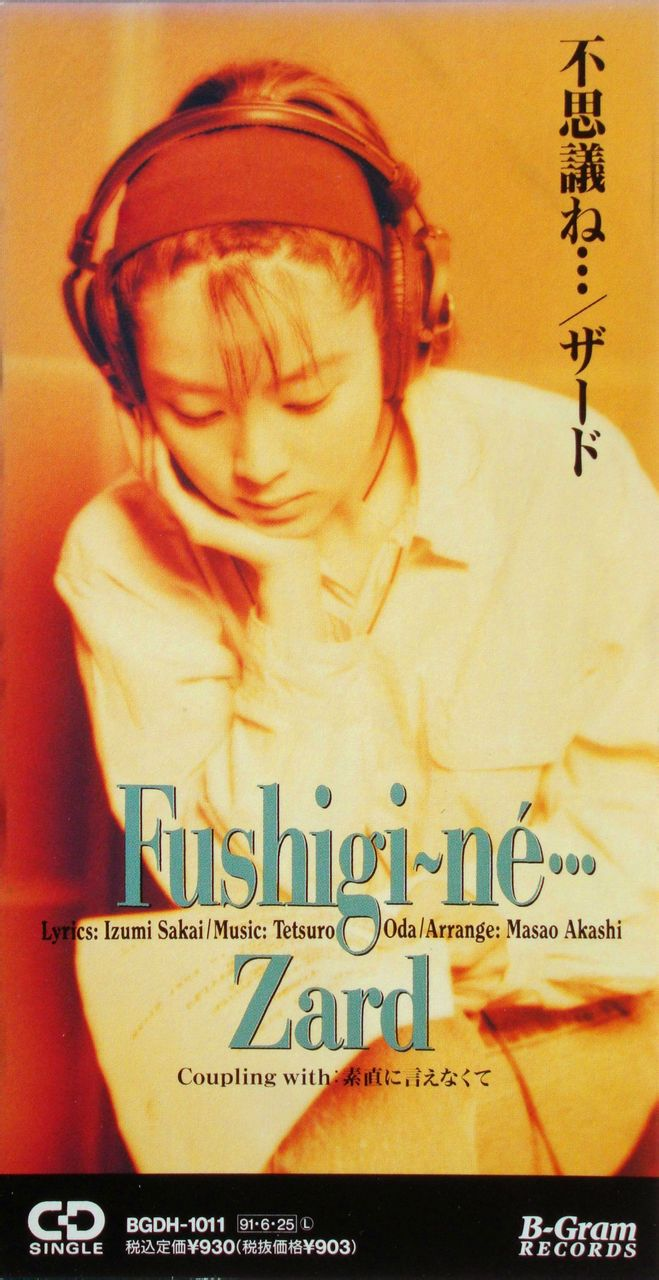
\includegraphics[width=0.3\textwidth]{S2.jpg}}

\large{

\ruby{夏}{なつ}の\ruby{風}{かぜ}が\ruby{素肌}{すはだ}に\ruby{キス}{Kiss}してる

\ruby{流}{なが}れてゆく\ruby{街並}{まちなみ}

すれ\ruby{違}{ちが}う\ruby{景色}{けしき}が\ruby{知}{し}らず\ruby{知}{し}らずのうちに

\ruby{崩}{くず}れてゆく サヨナラが\ruby{聴}{き}こえた
\\

ああ \ruby{季節}{とき}はすべてを\ruby{変}{か}えてしまう

\ruby{少年}{しょうねん}の\ruby{瞳}{ひとみ}を ずっと\ruby{忘}{わす}れないでね

\ruby{不思議}{ふしぎ}ね···\ruby{記憶}{きおく}は\ruby{空}{から}っぽにして

\ruby{壊}{こわ}れた\ruby{ハート}{Heart}をそっと\ruby{眠}{ねむ}らせて

in your dream
\\

\ruby{南風}{みなみかぜ}がやさしく\ruby{囁}{ささや}いている

\ruby{輝}{かがや}いていた あの\ruby{頃}{ころ}

さり\ruby{気}{げ}ない\ruby{仕草}{しぐさ}をいつも\ruby{横}{よこ}で\ruby{見}{み}ていた

これからは \ruby{遠}{とお}くで\ruby{気}{き}にしてる
\\

ああ \ruby{季節}{とき}はすべてを\ruby{変}{か}えてしまう

\ruby{言}{い}えなかった\ruby{悲}{かな}しみは \ruby{過}{す}ぎた\ruby{日}{ひ}の\ruby{幻}{まぼろし}

\ruby{不思議}{ふしぎ}ね···\ruby{記憶}{きおく}は\ruby{空}{から}っぽにして

\ruby{壊}{こわ}れた\ruby{ハート}{Heart}をそっと\ruby{眠}{ねむ}らせて in my dream
\\

ああ \ruby{季節}{とき}はすべてを\ruby{変}{か}えてしまう

せつない\ruby{想}{おも}い\ruby{出}{で}に \ruby{縛}{しば}られたくないの

\ruby{不思議}{ふしぎ}ね···\ruby{記憶}{きおく}は\ruby{空}{から}っぽにして

\ruby{壊}{こわ}れた\ruby{ハート}{Heart}をそっと\ruby{眠}{ねむ}らせて in my dream

}

\hypertarget{2_1}{}
\section{ もう探さない}

\large{

\ruby{灰色}{はいいろ}の\ruby{都会}{まち}を \ruby{見}{み}おろすこの\ruby{部屋}{へや}に

\ruby{無口}{むぐち}な\ruby{ノイズ}{Noise}\ruby{残}{のこ}して

\ruby{誰}{だれ}もいない…

\ruby{電話}{でんわ}も\ruby{鳴}{な}ることさえ \ruby{忘}{わす}れてる

\ruby{自由}{じゆう}になれた\ruby{痛}{いた}みね
\\

あの\ruby{夏}{なつ}の\ruby{日}{ひ}…

\ruby{子供}{こども}のように はしゃぐあなたが \ruby{眩}{まぶ}しかった

\ruby{遠}{とお}い\ruby{記憶}{きおく}
\\

\ruby{肩}{かた}を\ruby{寄}{よ}せて\ruby{歩}{ある}く \ruby{二人}{ふたり}の\ruby{コントラスト}{Contrast}

\ruby{溶}{と}け\ruby{合}{あ}うように\ruby{続}{つづ}いていた -もう\ruby{探}{さが}さない-

\ruby{熱}{あつ}く\ruby{生}{い}きることも ああ \ruby{少}{すこ}し\ruby{臆病}{おくびょう}になる

\ruby{裸}{はだか}のままで \ruby{今}{いま}は \ruby{愛}{あい}せないから
\\

\ruby{時}{とき}が\ruby{過}{た}てば いつも\ruby{切}{き}りかえは \ruby{得意}{とくい}なのに

\ruby{笑}{わら}っていても \ruby{苦}{くる}しい…

\ruby{年上}{としうえ}の\ruby{女}{ひと}と \ruby{暮}{く}らしていると\ruby{聞}{き}いた

もう\ruby{二度}{にど}と \ruby{電話}{だんわ}できない
\\

\ruby{少}{すこ}し\ruby{遥}{とお}く\ruby{見}{み}つめる\ruby{瞳}{ひとみ}

きっと あの\ruby{人}{ひと}を\ruby{映}{うつ}していた

\ruby{悲}{かな}しいけど
\\

\ruby{誰}{だれ}のせいでもない \ruby{運命}{とき}の\ruby{悪戯}{いたずら}だから

とり\ruby{戻}{もど}せない\ruby{微笑}{ほほえ}み -もう\ruby{探}{さが}さない-

\ruby{熱}{あつ}く\ruby{生}{い}きることも ああ \ruby{少}{すこ}し\ruby{臆病}{おくびょう}になる

あの\ruby{頃}{ころ}のように \ruby{今}{いま}は \ruby{帰}{かえ}れないから
\\

\ruby{肩}{かた}を\ruby{寄}{よ}せて\ruby{歩}{ある}く \ruby{二人}{ふたり}の\ruby{コントラスト}{Contrast}

\ruby{溶}{と}け\ruby{合}{あ}うように\ruby{続}{つづ}いていた -もう\ruby{探}{さが}さない-

\ruby{熱}{あつ}く\ruby{生}{い}きることも ああ \ruby{少}{すこ}し\ruby{臆病}{おくびょう}になる

\ruby{裸}{はだか}のままで \ruby{今}{いま}は \ruby{愛}{あい}せないから

}
{ \ }

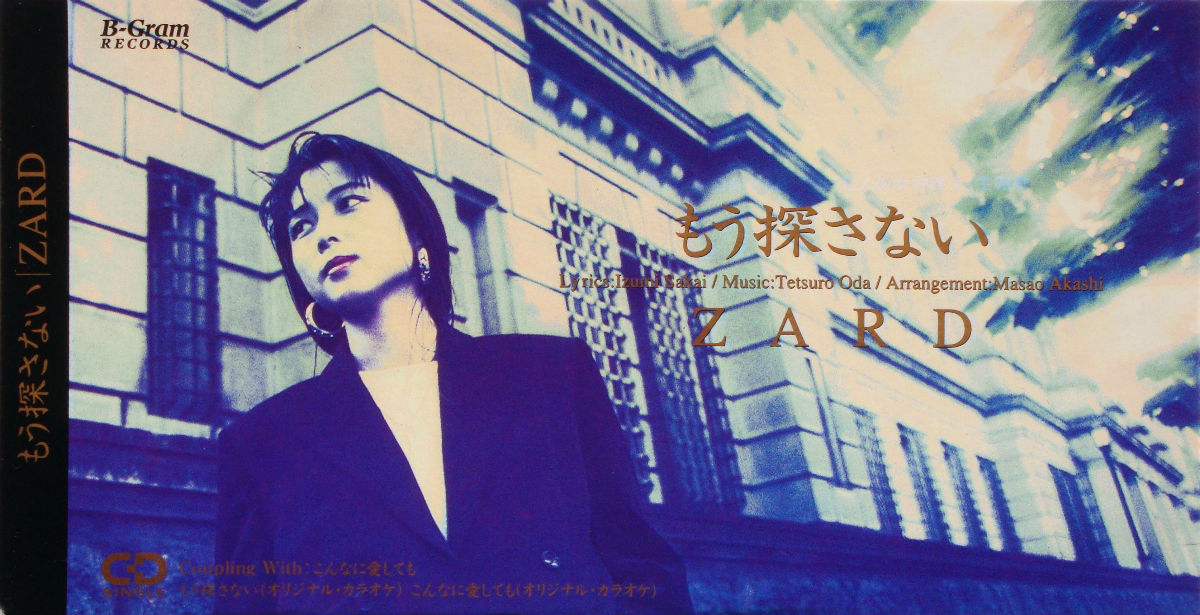
\includegraphics[width=0.5\textwidth]{S3.jpg}


\hypertarget{2_2}{}
\section{ 素直に言えなくて}
\large{

\ruby{星}{ほし}\ruby{降}{ふ}る\ruby{夜}{よる}は いつも Lonely-night

\ruby{溜}{た}め\ruby{息}{き}で \ruby{霞}{かす}んでる

\ruby{冷}{つめ}たい \ruby{ベッド}{bed}は \ruby{少}{すこ}し

\ruby{広}{ひろ}すぎて \ruby{眠}{ねむ}れない
\\

やさしすぎるから

つらくなってゆく

このまま ずっと \ruby{気付}{きづ}かないふりで

\ruby{笑顔}{えがお}に\ruby{変}{か}えたいの
\\

“ひとりにしないでね”って \ruby{素直}{すなお}に \ruby{言}{い}えなくて
\\

\parpic[r]{
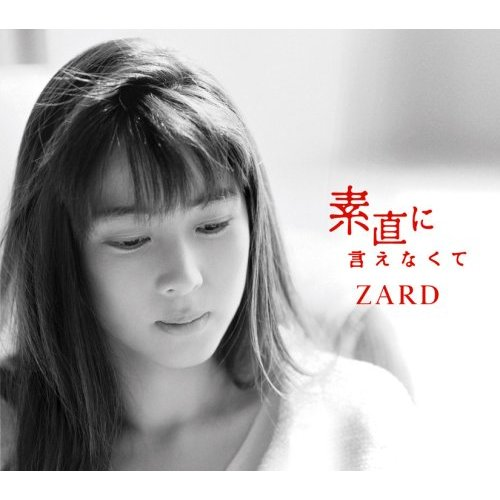
\includegraphics[width=0.4\textwidth]{S45.jpg}}

\ruby{腕}{うで}を\ruby{組}{く}んで \ruby{歩}{ある}いた Rainly-night

あたたかさに \ruby{酔}{よ}って

\ruby{夢}{ゆめ}を \ruby{見}{み}て いたいから

うしろは \ruby{振}{ふ}り\ruby{向}{む}かない
\\

\ruby{楽}{たの}しかったけど つらくなってゆく

これからは \ruby{強}{つよ}くなるから

きっと \ruby{涙}{なみだ}は \ruby{見}{み}せないわ
\\

“ひとりにしないでね”って \ruby{素直}{すなお}に \ruby{言}{い}えなくて
\\

やさしすぎるから つらくなってゆく

このまま ずっと \ruby{気付}{きづ}かないふりで

\ruby{笑顔}{えがお}に\ruby{変}{か}えたいの

“ひとりにしないでね”って \ruby{素直}{すなお}に \ruby{言}{い}えなくて

}

\hypertarget{2_3}{}
\section{ ひとりが好き}
\large{

\ruby{思}{おも}い\ruby{出}{だ}すの \ruby{初}{はじ}めての

kissを\ruby{交}{か}わした \ruby{メリークリスマス}{merry Xmas}

\ruby{今}{いま}\ruby{思}{おも}えば \ruby{懐}{なつ}かしい\ruby{嘘}{うそ}

“キミだけだよ”なんて\ruby{信}{しん}じて…
\\

もう\ruby{気}{き}にしないで ひとりが こんなに\ruby{好}{す}き
\\

\ruby{愛}{あい}して \ruby{見}{み}えなくなるよりは

\ruby{距離}{はな}れていた\ruby{方}{ほう}がいい

\ruby{近}{ちか}くて \ruby{遠}{とお}すぎる

あなたの\ruby{影}{かげ}を \ruby{抱}{だ}いて
\\

\ruby{歩}{ある}き\ruby{出}{だ}した \ruby{想}{おも}い\ruby{出}{で}は

\ruby{銀色}{ぎんいろ}の\ruby{街}{まち}に \ruby{紛}{まぎ}れて

こぼれ\ruby{落}{お}ちた \ruby{涙}{なみだ}の\ruby{数}{かず}

あなたを\ruby{思}{おも}う\ruby{深}{ふか}さなのね
\\

もう\ruby{気}{き}にしないで ひとりが こんなに\ruby{好}{す}き
\\

\ruby{愛}{あい}して やさしさを\ruby{失}{うしな}うよりは

\ruby{見}{み}つめていたい

\ruby{近}{ちか}くて \ruby{遠}{とお}すぎる

あなたの\ruby{影}{かげ}を \ruby{抱}{だ}いて
\\

\ruby{愛}{あい}して やさしさを\ruby{失}{うしな}うよりは

\ruby{見}{み}つめていたい

\ruby{近}{ちか}くて \ruby{遠}{とお}すぎる

あなたの\ruby{影}{かげ}を \ruby{抱}{だ}いて

}

\hypertarget{2_4}{}
\section{ Forever}
\large{

\ruby{霞}{かす}む\ruby{街並}{まちな}みに

ざわめく\ruby{朝}{あさ}は

あなたの\ruby{香}{かお}りで

\ruby{夢}{ゆめ}から\ruby{覚}{さ}めてゆく

\ruby{出逢}{であ}いと\ruby{別}{わか}れは

いつでも…

\ruby{プリズム}{prism}

\ruby{色褪}{いろあ}せた\ruby{想}{おも}い

\ruby{眩}{まぶ}しいほど\ruby{弾}{はじ}くよ
\\

\ruby{変}{か}わらぬ

\ruby{恋}{こい}の\ruby{約束}{やくそく}

あの\ruby{場所}{ばしょ}に\ruby{置}{お}き\ruby{去}{さ}りのまま

\ruby{信}{しん}じることの\ruby{強}{つよ}さを

この\ruby{胸}{むね}に\ruby{抱}{だ}きしめて

love you forever, you
\\

\ruby{蒼}{あお}い\ruby{月明}{つきあ}かり

\ruby{静}{しず}かに\ruby{照}{て}らす

“ねぇ

\ruby{素直}{すなお}な\ruby{瞳}{め}で

\ruby{明日}{あした}を\ruby{見}{み}つめようよ”

たとえ\ruby{苦}{くる}しい\ruby{思}{おも}い\ruby{出}{で}も…

\ruby{宝石}{ほうせき}

\ruby{懐}{なつ}かしく\ruby{光}{ひかる}

いつか\ruby{消}{き}えてゆく

あの\ruby{日}{ひ}に
\\

\ruby{傷}{きず}つけ\ruby{会}{あ}う\ruby{悲}{かな}しみは

ああ

\ruby{涙}{なみだ}で\ruby{癒}{いや}せるから

\ruby{愛}{あい}し\ruby{続}{つづ}ける\ruby{勇気}{ゆうき}を

いつまでも\ruby{忘}{わす}れないで

love you forever, you
\\

\ruby{変}{か}わらぬ

\ruby{恋}{こい}の\ruby{約束}{やくそく}

あの\ruby{場所}{ばしょ}に\ruby{置}{お}き\ruby{去}{さ}りのまま

\ruby{信}{しん}じることの\ruby{強}{つよ}さを

この\ruby{胸}{むね}に\ruby{抱}{だ}きしめて
\\

\ruby{傷}{きず}つけ\ruby{会}{あ}う\ruby{悲}{かな}しみは

ああ

\ruby{涙}{なみだ}で\ruby{癒}{いや}せるから

\ruby{愛}{あい}し\ruby{続}{つづ}ける\ruby{勇気}{ゆうき}を

いつまでも\ruby{忘}{わす}れないで

love you forever, you

}

\hypertarget{2_5}{}
\section{ Lonely soldier boy}
\large{

Just relax leave it to me…

I can say, I love you…
\\

\ruby{出会}{であ}いは \ruby{必然}{ひつぜん}ね

\ruby{瞳}{ひとみ} \ruby{覗}{のぞ}いて 「\ruby{愛}{あい}してる」

や·さ·し·く \ruby{攻}{せ}めないで

\ruby{今日}{きょう}はどうにかなりそう
\\

\ruby{誰}{だれ}かにきっと\ruby{甘}{あま}えているのね

いじらしい\ruby{手}{て}をさしのべてる

\ruby{媚薬}{びやく}の\ruby{体}{かなだ} \ruby{守}{まも}ってあげたいけど

\ruby{強}{つよ}がってる
\\

\ruby{振}{ふ}り\ruby{向}{む}かないで Lonely soldier boy

\ruby{傷}{きず}ついた\ruby{背中}{せなか}を \ruby{癒}{いや}すまで

\ruby{立}{た}ち\ruby{止}{ど}まらないで \ruby{笑}{わら}ってよ

a lonely, lonely,

Lonely soldier boy
\\

\ruby{欲}{ほ}しがる\ruby{唇}{くちびる}で

\ruby{恋}{こい}の\ruby{手口}{てぐち}は イかしてた

やさちく\ruby{腰}{こし}を\ruby{抱}{だ}けば

\ruby{少}{すこ}し\ruby{長}{なが}めの makin' love
\\

\ruby{不埒}{ふらち}な\ruby{視線}{しせん} \ruby{指}{ゆび}を\ruby{鳴}{な}らして

\ruby{慣}{な}れあう\ruby{愛}{あい}を \ruby{求}{もと}めてる

\ruby{螺旋}{らせん}の\ruby{爪}{つめ}で\ruby{守}{まも}ってあげたいから

\ruby{強}{つよ}がっても
\\

\ruby{怖}{こわ}がらないで Lonely soldier boy

\ruby{傷}{きず}つけた\ruby{青}{あお}さに \ruby{気}{き}づくまで

\ruby{立}{た}ち\ruby{止}{ど}まらないで \ruby{笑}{わら}ってよ

a lonely, lonely,

Lonely soldier boy
\\

\ruby{乾}{かわ}いたのノド\ruby{叫}{さけ}ぶ

Ah \ruby{踊}{おど}らせて \ruby{腕}{うで}の\ruby{中}{なか}で

\ruby{悩}{なや}ましく \ruby{胸元}{むなもと}に

\ruby{飢}{う}えた\ruby{顔}{かお}を\ruby{埋}{うず}めて
\\

\ruby{振}{ふ}り\ruby{向}{む}かないで Lonely soldier boy

\ruby{傷}{きず}ついた\ruby{背中}{せなか}を \ruby{癒}{いや}すまで

\ruby{立}{た}ち\ruby{止}{ど}まらないで \ruby{笑}{わら}ってよ

a lonely, lonely,

Lonely soldier boy
\\

\ruby{怖}{こわ}がらないで Lonely soldier boy

\ruby{傷}{きず}つけた\ruby{青}{あお}さに \ruby{気}{き}づくまで

\ruby{立}{た}ち\ruby{止}{ど}まらないで \ruby{笑}{わら}ってよ

a lonely, lonely,

Lonely soldier boy

}

\hypertarget{2_6}{}
\section{ いつかは}
\large{

Baby, Baby don't you cry

\ruby{静}{しず}かな\ruby{夕暮}{ゆうぐ}れに

\ruby{残}{のこ}された\ruby{日々}{ひび} \ruby{夢}{ゆめ}を\ruby{見}{み}させて

どんなに\ruby{時間}{とき}を \ruby{縛}{しば}ってもほどける

あとどれくらい \ruby{生}{い}きられるのか
\\

いつかは\ruby{情熱}{じょうねつ}も \ruby{記憶}{きおく}の\ruby{底}{そこ}へ

\ruby{愛}{あい}し\ruby{合}{あ}う\ruby{二人}{ふたり}も \ruby{セピア}{sepia}に\ruby{変}{か}わる
\\

Baby, Baby don't you cry

\ruby{願}{ねが}いがかなうなら

あなたと\ruby{共}{とも}に \ruby{輝}{かがや}きたいの
\\

いつかは\ruby{新}{あたら}しい\ruby{恋}{こい}に おぼれる

\ruby{過}{す}ぎゆく\ruby{季節}{きせつ}さえ \ruby{気付}{きづ}かないまま

いつかは\ruby{情熱}{じょうねつ}も \ruby{記憶}{きおく}の\ruby{底}{そこ}へ

\ruby{愛}{あい}し\ruby{合}{あ}う\ruby{二人}{ふたり}も \ruby{セピア}{sepia}に\ruby{変}{か}わる
\\

Baby, Baby don't you cry

\ruby{忘}{わす}れないで ずっと

あなたの\ruby{中}{なか}に \ruby{生}{い}き\ruby{続}{つづ}けるわ

Baby, Baby don't you cry

}

\chapter{Album 3}
\thispagestyle{empty} %本页頁碼空白
\vspace{-16mm}
\LARGE {HOLD ME}

\normalsize{BGCH-1005 1992.9.2 \ release}
\\

\vspace{-5mm}

\parpic[l]{
\pichskip{6em}
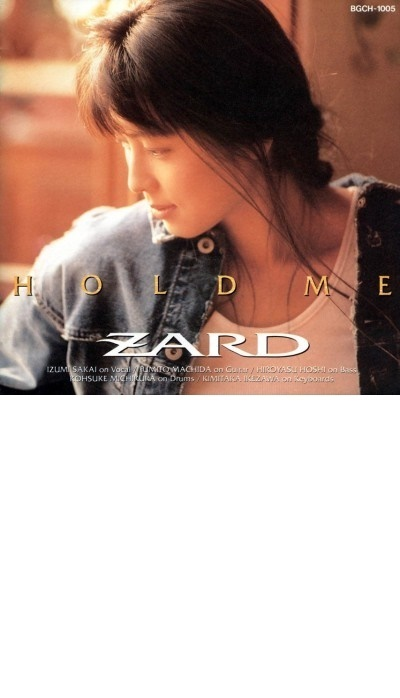
\includegraphics[width=0.4\textwidth]{3.jpg}}

\small{\hyperlink{3_0}{1.眠れない夜を抱いて}}

\tiny{作詞:坂井泉水 \ 作曲:織田哲郎 \ 編曲:明石昌夫/池田大介}

\small{\hyperlink{3_1}{2.誰かが待ってる}}

\tiny{作詞:坂井泉水 \ 作曲:栗林誠一郎 \ 編曲:明石昌夫}

\small{\hyperlink{3_2}{3.サヨナラ言えなくて}}

\tiny{作詞:坂井泉水 \ 作曲:栗林誠一郎 \ 編曲:池田大介}

\small{\hyperlink{3_3}{4.あの微笑みを忘れないで}}

\tiny{作詞:坂井泉水 \ 作曲:川島だりあ \ 編曲:明石昌夫}

\small{\hyperlink{3_4}{5.好きなように踊りたいの}}

\tiny{作詞:坂井泉水 \ 作曲:和泉一弥 \ 編曲:葉山たけし}

\small{\hyperlink{3_5}{6.Dangerous Tonight}}

\tiny{作詞:坂井泉水 \ 作曲:栗林誠一郎 \ 編曲:明石昌夫}

\small{\hyperlink{3_6}{7.こんなに愛しても}}

\tiny{作詞:坂井泉水 \ 作曲:栗林誠一郎 \ 編曲:明石昌夫}

\small{\hyperlink{3_7}{8.Why Don't You Leave Me Alone}}

\tiny{作詞:坂井泉水 \ 作曲:川島だりあ \ 編曲:葉山たけし}

\small{\hyperlink{3_8}{9.愛は眠ってる}}

\tiny{作詞:坂井泉水 \ 作曲:川島だりあ \ 編曲:池田大介}

\small{\hyperlink{3_9}{10.遠い日のNostalgia}}

\tiny{作詞:坂井泉水 \ 作曲:望月衛介 \ 編曲:明石昌夫}

\small{\hyperlink{3_10}{11.So Together}}

\tiny{作詞:坂井泉水 \ 作曲:川島だりあ \ 編曲:明石昌夫}

\small{ \ }

\tiny{ \ }

\clearpage

\hypertarget{3_0}{}
\section{ 眠れない夜を抱いて}
\large{

ざわめく\ruby{都会}{まち}の\ruby{景色}{けしき}が\ruby{止}{と}まる

あの\ruby{日}{ひ}\ruby{見}{み}たデ·ジャ·ヴと\ruby{重}{かさ}なる\ruby{影}{かげ}

もしもあの\ruby{時}{とき} \ruby{出逢}{であ}わなければ

\ruby{傷}{きず}つけ\ruby{合}{あ}うことを \ruby{知}{し}らなかった
\\

いじわるに\ruby{言葉}{ことば}はすれ\ruby{違}{ちが}うけど

\ruby{愛}{あい}を\ruby{求}{もと}めてる
\\

\ruby{眠}{ねむ}れない\ruby{夜}{よる}を\ruby{抱}{だ}いて

\ruby{不思議}{ふしぎ}な\ruby{世界}{せかい}へと\ruby{行}{ゆ}く

まだ\ruby{少女}{しょうじょ}の\ruby{頃}{ころ}の

あどけない\ruby{笑顔}{えがお}に\ruby{戻}{もど}って

in my dream mystery
\\

こぼれた\ruby{夢}{ゆめ}のカケラをすくって

\ruby{慣}{な}れてゆく\ruby{毎日}{まいにち}を\ruby{確}{たし}かめてゆく

もしもあの\ruby{時}{とき} \ruby{少}{すこ}し\ruby{大人}{おとな}になってたら

サヨナラ\ruby{言}{い}えなかった
\\

\ruby{解}{と}けてゆく\ruby{孤独}{こどく}な\ruby{心}{こころ}はいつも

\ruby{愛}{あい}を\ruby{求}{もと}めてる
\\

\ruby{眠}{ねむ}れない\ruby{夜}{よる}を\ruby{抱}{だ}いて

\ruby{駆}{か}け\ruby{抜}{ぬ}けた\ruby{時間}{とき}を\ruby{想}{おも}うの

まだ\ruby{少女}{しょうじょ}の\ruby{頃}{ころ}の

あどけない\ruby{笑顔}{えがお}に\ruby{戻}{もど}って

in my dream mystery
\\

\ruby{眠}{ねむ}れない\ruby{夜}{よる}を\ruby{抱}{だ}いて

\ruby{不思議}{ふしぎ}な\ruby{世界}{せかい}へと\ruby{行}{ゆ}く

まだ\ruby{少女}{しょうじょ}の\ruby{頃}{ころ}の

あどけない\ruby{笑顔}{えがお}に\ruby{戻}{もど}って

in my dream mystery
\\

\ruby{眠}{ねむ}れない\ruby{夜}{よる}を\ruby{抱}{だ}いて

\ruby{駆}{か}け\ruby{抜}{ぬ}けた\ruby{時間}{とき}を\ruby{想}{おも}うの

まだ\ruby{少女}{しょうじょ}の\ruby{頃}{ころ}の

あどけない\ruby{笑顔}{えがお}に\ruby{戻}{もど}って

in my dream mystery

}
{ \ }

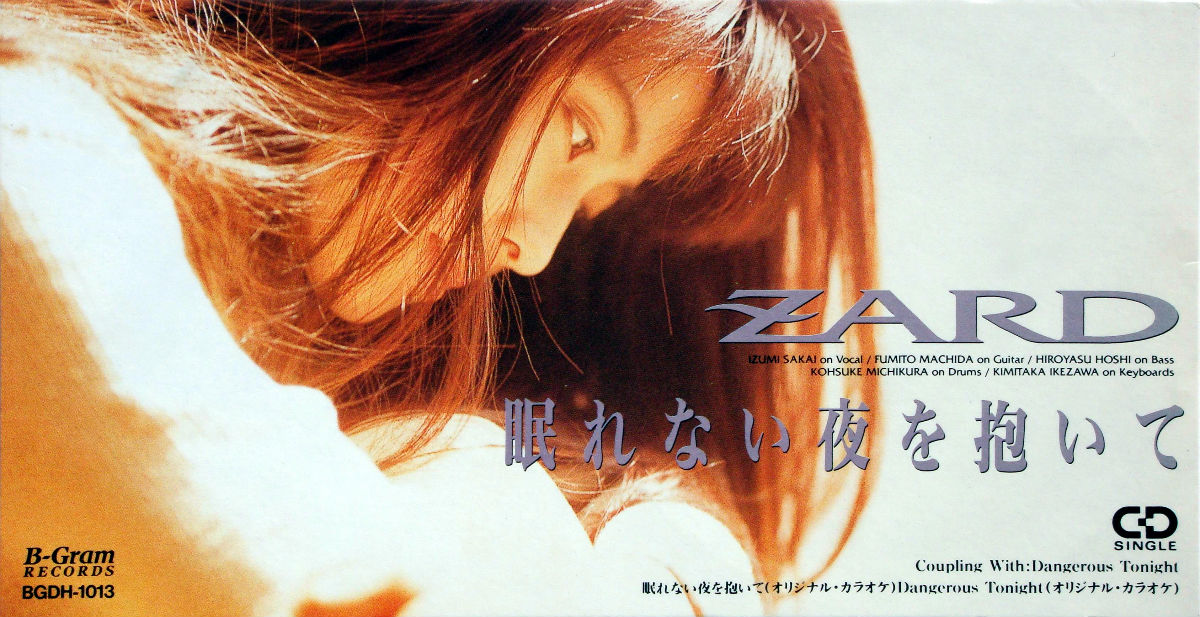
\includegraphics[width=0.5\textwidth]{S4.jpg}

\hypertarget{3_1}{}
\section{ 誰かが待ってる}
\large{

\ruby{見慣}{みな}れた\ruby{ビル}{building}を\ruby{背}{せ}に

\ruby{近付}{ちかづ}く\ruby{足音}{あしおと}

「\ruby{元気}{げんき}か」と\ruby{無邪気}{むじゃき}に\ruby{問}{と}いかける

まるで\ruby{初}{はじ}めて\ruby{会}{あ}ったように

\ruby{眩}{まぶ}しい\ruby{瞳}{ひとみ}が\ruby{憎}{にく}らしい…
\\

ときめく\ruby{思}{おも}い\ruby{出}{で}\ruby{心}{こころ}を\ruby{飾}{かざ}れば 

\ruby{微笑}{ほほえ}む\ruby{私}{わたし}を\ruby{誰}{だれ}かが\ruby{待}{ま}ってる
\\

いつもぜいたくな\ruby{言葉}{ことば}におびえてた

サヨナラが\ruby{レアル}{real}に\ruby{笑}{わら}うの

\ruby{愛}{あい}していたこと… \ruby{忘}{わす}れない

すべてが\ruby{夢}{ゆめ}に\ruby{変}{か}わっても
\\

\ruby{一番}{いちばん}\ruby{大切}{たいせつ}な\ruby{優}{やさ}しさをあげる

\ruby{振}{ふ}り\ruby{向}{む}く\ruby{私}{わたし}を\ruby{誰}{だれ}かが\ruby{待}{ま}ってる
\\

ときめく\ruby{思}{おも}い\ruby{出}{で}\ruby{心}{こころ}を\ruby{飾}{かざ}れば 

\ruby{微笑}{ほほえ}む\ruby{私}{わたし}を\ruby{誰}{だれ}かが\ruby{待}{ま}ってる
\\

\ruby{一番}{いちばん}\ruby{大切}{たいせつ}な\ruby{優}{やさ}しさをあげる

\ruby{振}{ふ}り\ruby{向}{む}く\ruby{私}{わたし}を\ruby{誰}{だれ}かが\ruby{待}{ま}ってる

}

\hypertarget{3_2}{}
\section{ サヨナラ言えなくて}
\large{

\ruby{窓}{まど}ににじむ city lights

ぼんやり\ruby{雨}{あめ}の\ruby{音}{おと}を\ruby{楽}{たの}しんでる

\ruby{長過}{ながす}ぎる\ruby{夜}{よる}の\ruby{過}{す}ごしかた

うまくなった上手みたい
\\

\ruby{優}{やさ}し\ruby{過}{す}ぎた\ruby{別}{わか}れの\ruby{言葉}{ことば}が

\ruby{今}{いま}も\ruby{蘇}{よみがえ}る memory

まだどこかで\ruby{思}{おも}い\ruby{出}{で}の\ruby{中}{なか}の

あなたを\ruby{探}{さが}してる
\\

\ruby{目覚}{めざ}めの\ruby{コーヒー}{coffee}\ruby{苦}{にが}く\ruby{飲}{の}みほす

\ruby{朝}{あさ}の\ruby{景色}{けしき}\ruby{霞}{かす}んでる

\ruby{今}{いま}ごろどうしているのかと

\ruby{カレンダー}{calendar}を\ruby{望}{のぞ}く
\\

\ruby{最後}{さいご}の\ruby{夏}{なつ}\ruby{鮮}{あざ}やかな shiny blue

\ruby{胸}{むね}の\ruby{奧}{おく}が\ruby{切}{せつ}ない story

まだどこかであなたを\ruby{待}{ま}ってる

サヨナラ\ruby{言}{い}えなくて
\\

\ruby{最後}{さいご}の\ruby{夏}{なつ}\ruby{鮮}{あざ}やかな shiny blue

\ruby{胸}{むね}の\ruby{奧}{おく}が\ruby{切}{せつ}ない story

まだどこかであなたを\ruby{待}{ま}ってる

サヨナラ\ruby{言}{い}えなくて

}

\hypertarget{3_3}{}
\section{ あの微笑みを忘れないで}
\large{

あの\ruby{微笑}{ほほえ}みを\ruby{忘}{わす}れないで

Forget your worries and gimme your smile

\ruby{心}{こころ}の\ruby{冬}{ふゆ}にさよならして

\ruby{走}{はし}り\ruby{出}{だ}そう \ruby{新}{あたら}しい\ruby{明日}{あした}へ
\\

\ruby{25時}{にじゅうごじ} \ruby{砂}{すな}の\ruby{上}{うえ}に\ruby{車}{くるま}\ruby{止}{と}めて

\ruby{語}{かた}り\ruby{明}{あか}かしたあの\ruby{夏}{なつ}

ぬるいコーラしかなくても

\ruby{夢}{ゆめ}だけで\ruby{樂}{たの}しかった

\ruby{思}{おも}い\ruby{出}{だ}して…

つまづいた\ruby{時}{とき}には \ruby{電話}{でんわ}をしてね
\\

Open your heart \ruby{風}{かぜ}を\ruby{感}{かん}じて

あきらめを\ruby{手}{て}にしないで

\ruby{都會}{とかい}がくれた ポーカーface

\ruby{海}{うみ}に\ruby{捨}{す}ててしまおう

あの\ruby{微笑}{ほほえ}みを\ruby{忘}{わす}れないで いつも\ruby{輝}{かがや}いてたい

\ruby{心}{こころ}の\ruby{冬}{ふゆ}にさよならして

\ruby{走}{はし}り\ruby{出}{だ}そう \ruby{新}{あたら}しい\ruby{明日}{あした}へ
\\

レンガ\ruby{色}{いろ}の\ruby{空}{そら}を\ruby{斜}{なな}めに\ruby{見}{み}\ruby{上}{あ}げて

\ruby{口笛}{くちぶえ}\ruby{吹}{ふ}いた my home town

やりたいこと \ruby{欲}{ほ}しいものも

\ruby{抱}{だか}えきれないほどで

\ruby{切}{せつ}なさのハードル\ruby{超}{こ}えられたね

\ruby{今}{いま}も\ruby{出來}{でき}るよ
\\

Open your heart ひたむきな

あなたの\ruby{瞳}{め}が好きだった

\ruby{孤獨}{こどく}な\ruby{時間}{じかん}\ruby{抱}{だ}きしめて

\ruby{人}{ひと}は\ruby{大人}{おとな}になるから

あの\ruby{微笑}{ほほえ}みを\ruby{忘}{わす}れないで いつも\ruby{輝}{かがや}いてたい

もう\ruby{何}{なに}も\ruby{迷}{まよ}うことなく

\ruby{走}{はし}り\ruby{出}{だ}そう \ruby{新}{あたら}しい\ruby{明日}{あした}へ
\\

You've got to open your heart

When ever you feel blue

Forget your worries and gimme your smile
\\

\ruby{心}{こころ}の\ruby{冬}{ふゆ}にさよならして

\ruby{走}{はし}り\ruby{出}{だ}そう \ruby{新}{あたら}しい\ruby{明日}{あした}へ
\\

You've got to open your heart \ruby{風}{かぜ}を\ruby{感}{かん}じて

あきらめを\ruby{手}{て}にしないで

\ruby{都會}{とかい}がくれた ポーカーface

\ruby{海}{うみ}に\ruby{捨}{す}ててしまおう

あの\ruby{微笑}{ほほえ}みを\ruby{忘}{わす}れないで いつも\ruby{輝}{かがや}いてたい

\ruby{心}{こころ}の\ruby{冬}{ふゆ}にさよならして

\ruby{走}{はし}り\ruby{出}{だ}そう \ruby{新}{あたら}しい\ruby{明日}{あした}へ

}

\hypertarget{3_4}{}
\section{ 好きなように踊りたいの}
\large{

\ruby{気}{き}が\ruby{付}{つ}いたら\ruby{私}{わたし}

\ruby{振}{ふ}りまわされてる

\ruby{デート}{date}の\ruby{キャンセル}{cancel}だって

\ruby{怪}{あや}しいにおいが
\\

「もうあなたの\ruby{ジョーク}{joke}じゃ

\ruby{笑}{わら}えないわよ」と

\ruby{映画}{えいが}のセリフ\ruby{真似}{まね}して

\ruby{冷}{つめ}たく\ruby{言}{い}おう
\\

\ruby{瞳}{ひとみ}だけで\ruby{話}{はな}したね

\ruby{出会}{であ}ったあの\ruby{頃}{ころ}は

でも\ruby{自由}{じゆう}が\ruby{欲}{ほ}しいよ どうする?

oh darling!
\\

\ruby{好}{す}きなように\ruby{踊}{おど}りたいの

あなたの\ruby{手}{て}を\ruby{離}{はな}れて

\ruby{好}{す}きなように\ruby{踊}{おど}りたいの

\ruby{ヒール}{heel}\ruby{脱}{ぬ}ぎ\ruby{捨}{す}てたらもう

\ruby{洋服}{ようふく}も\ruby{趣味}{しゅみ}を\ruby{変}{か}えて

\ruby{自分}{じぶん}のためにおしゃれ oh

\ruby{手遅}{ておく}れにならないといいけどね
\\

\ruby{留守電}{るすでん}には

あなたの\ruby{不機嫌}{ふきげん}な\ruby{声}{こえ}が

せっかくだけど

\ruby{他}{ほか}で\ruby{間}{ま}に\ruby{合}{あ}わせてよ
\\

まるで\ruby{二人}{ふたり}だけの\ruby{シーサイド}{seaside}

\ruby{出会}{であ}ったあの\ruby{頃}{ころ}は

でも\ruby{世界}{せかい}は\ruby{一人}{ひとり}と

\ruby{気}{き}が\ruby{付}{つ}いた

oh darling!
\\

\ruby{好}{す}きなように\ruby{踊}{おど}りたいの

\ruby{一人}{ひとり}だけの\ruby{ステップ}{step}で

\ruby{好}{す}きなように\ruby{踊}{おど}りたいの

すこし\ruby{反省}{はんせい}するなら…

\ruby{戻}{もど}るかもしれないし

\ruby{戻}{もど}らないかもしれない oh

\ruby{愛情}{あいじょう}の\ruby{ボルテージ}{voltage}を\ruby{確}{たし}かめて
\\

\ruby{好}{す}きなように\ruby{踊}{おど}りたいの

あなたの\ruby{手}{て}を\ruby{離}{はな}れて

\ruby{好}{す}きなように\ruby{踊}{おど}りたいの

\ruby{ヒール}{heel}\ruby{脱}{ぬ}ぎ\ruby{捨}{す}てたらもう

\ruby{洋服}{ようふく}も\ruby{趣味}{しゅみ}を\ruby{変}{か}えて

\ruby{自分}{じぶん}のためにおしゃれ oh

\ruby{手遅}{ておく}れにならないといいけどね
\\

\ruby{好}{す}きなように\ruby{踊}{おど}りたいの

\ruby{一人}{ひとり}だけの\ruby{ステップ}{step}で

\ruby{好}{す}きなように\ruby{踊}{おど}りたいの

すこし\ruby{反省}{はんせい}するなら…

\ruby{戻}{もど}るかもしれないし

\ruby{戻}{もど}らないかもしれない oh

\ruby{愛情}{あいじょう}の\ruby{ボルテージ}{voltage}を\ruby{確}{たし}かめて

}

\hypertarget{3_5}{}
\section{ Dangerous Tonight}
\large{

\ruby{燒}{や}けつく\ruby{日射}{ひざ}しに\ruby{感}{かん}じたgeneration

\ruby{海辺}{うみべ}のjealousy \ruby{背中}{せなか}に\ruby{独}{ひと}りじめ

あなたはsurfer boy \ruby{上手}{うわて}の\ruby{笑顔}{えがお}で

Jokeと \ruby{駆引}{かけひ}き\ruby{甘}{あま}いgameの\ruby{始}{はじ}まり
\\

Dangerous Tonight

\ruby{濡}{ぬ}れた\ruby{唇}{くちびる}みだされ

うそを\ruby{許}{ゆ}るしてもいいと…

So なにもかも\ruby{嫌}{いや}になるほど

\ruby{激}{はげ}しく\ruby{抱}{だ}きたいの
\\

\ruby{大人}{おとな}のふりしてもいかれてく

Feel my heart beat

\ruby{二度目}{にどめ}の\ruby{季節}{きせつ}も\ruby{超}{こ}えたい

あなたと\ruby{一緖}{いっしょ}に
\\

Dangerous Tonight

\ruby{絡}{から}みつく\ruby{指先}{ゆびさき}に\ruby{意味}{いみ}はあるの?

I want to know

もう\ruby{何}{なに}もかも\ruby{嫌}{いや}になるほど

\ruby{愛}{あい}して\ruby{夢}{ゆめ}をみさせて
\\

Dangerous Tonight

\ruby{絡}{から}みつく\ruby{指先}{ゆびさき}に\ruby{意味}{いみ}はあるの?

I want to know

もう\ruby{何}{なに}もかも\ruby{嫌}{いや}になるほど

\ruby{愛}{あい}して\ruby{夢}{ゆめ}をみさせて

}

\hypertarget{3_6}{}
\section{ こんなに愛しても}
\large{

\ruby{約束}{やくそく}\ruby{忘}{わす}れたの?

\ruby{真夜中}{まよなか}すぎの あなたの\ruby{部屋}{へや}で

\ruby{過}{す}ぎてく\ruby{時間}{じかん}を ただ\ruby{待}{ま}ってる

いつの\ruby{間}{ま}にか \ruby{眠}{ねむ}ってた
\\

こんなに\ruby{愛}{あい}しても

\ruby{時々}{ときどき}\ruby{淋}{さみ}しい\ruby{顔}{かお}するのね

\ruby{"何}{なに}かが\ruby{足}{た}りない"そんな\ruby{風}{ふう}ね

もどかしさに \ruby{不安}{ふあん}になる
\\

Hold Me そばにいて

やさしくなくても かまわないの

Love Me もう\ruby{二度}{にどと}と

\ruby{他}{ほか}の\ruby{誰}{だれ}かを \ruby{愛}{あい}さないで
\\

こんなに\ruby{愛}{あい}しても

\ruby{心}{こころ}はあなたに\ruby{届}{とど}かない

\ruby{出逢}{であ}った\ruby{頃}{ころ}を\ruby{思}{おも}い\ruby{出}{だ}して

またひとりで \ruby{切}{せつ}なくなる
\\

Hold Me そばにいて

\ruby{上手}{きよう}な\ruby{言葉}{ことば}は\ruby{要}{い}らないから

Love Me もう\ruby{二度}{にどと}と

\ruby{他}{ほか}の\ruby{誰}{だれ}かを \ruby{愛}{あい}さないで
\\

Hold Me そばにいて

やさしくなくても かまわないの

Love Me もう\ruby{二度}{にどと}と

\ruby{他}{ほか}の\ruby{誰}{だれ}かを \ruby{愛}{あい}さないで

}

\hypertarget{3_7}{}
\section{ Why don't you leave me alone}
\large{

\ruby{凍}{こお}り\ruby{付}{つ}く\ruby{アスファルト}{asphalt}に

\ruby{鳴}{な}りひびくハイヒル

\ruby{眠}{ねむ}らない\ruby{町}{まち} \ruby{見知}{みし}らぬ\ruby{人}{ひと}さま\ruby{迷}{まよ}い

\ruby{何度}{なんど}も\ruby{重}{かさ}ねた\ruby{夜}{よる}に\ruby{感}{かん}じていても

\ruby{別}{べつ}の\ruby{瞳}{ひとみ}に\ruby{映}{うつ}るあなた\ruby{確}{たし}かめてた
\\

\ruby{強}{つよ}がることも\ruby{忘}{わす}れて

ただ\ruby{退屈}{たいくつ}に\ruby{微笑}{ほほえ}む

\ruby{淋}{さび}しさにはなれなくて

Why don't you leave me alone tonight
\\

\ruby{通}{とお}り\ruby{過}{す}ぎる\ruby{冬}{ふゆ}の\ruby{風}{かぜ}は

\ruby{切}{せつ}なく\ruby{泣}{な}いて

\ruby{空}{むな}しい\ruby{愛}{あい}をせめることも\ruby{孤独}{こどく}すぎて
\\

\ruby{震}{ふる}える\ruby{体}{からだ}\ruby{抱}{だ}きしめて

\ruby{覚}{さ}めた\ruby{笑顔}{えがお}つくるけど

\ruby{淋}{さび}しさにはなれなくて

Why don't you leave me alone tonight
\\

\ruby{強}{つよ}がることも\ruby{忘}{わす}れて

ただ\ruby{退屈}{たいくつ}に\ruby{微笑}{ほほえ}む

\ruby{淋}{さび}しさにはなれなくて

Why don't you leave me alone tonight
\\

\ruby{震}{ふる}える\ruby{体}{からだ}\ruby{抱}{だ}きしめて

\ruby{覚}{さ}めた\ruby{笑顔}{えがお}つくるけど

\ruby{淋}{さび}しさにはなれなくて

Why don't you leave me alone tonight

}

\hypertarget{3_8}{}
\section{ 愛は眠ってる}
\large{

\ruby{音}{おと}もなく\ruby{月明}{つきあか}り

\ruby{不思議}{ふしぎ}\ruby{色}{いろ}に\ruby{変}{か}わって\ruby{行}{ゆ}く

\ruby{遥}{はる}かに\ruby{遠}{とお}い\ruby{過去}{かこ}の\ruby{愛}{あい}を

\ruby{信}{しん}じていたい

でももう\ruby{戻}{もど}れないと for me

どこかで\ruby{感}{かん}じてる
\\

Broken Heart \ruby{永遠}{えいえん}の\ruby{願}{ねが}いは

\ruby{未来}{みらい}へと\ruby{続}{つづ}く

Broken Heart  \ruby{時}{とき}の\ruby{流}{なが}れ\ruby{抱}{だ}いて

\ruby{愛}{あい}は\ruby{眠}{ねむ}ってる
\\

\ruby{気}{き}の\ruby{弱}{よわ}い\ruby{ラジオ}{radio}から

\ruby{聞}{き}こえてくるあの\ruby{ラブソング}{love song}

Winding Road \ruby{走}{はし}り\ruby{続}{つづ}けてた

あの\ruby{日}{ひ}の\ruby{二人}{ふたり}を\ruby{見}{み}つめ

なぜそんなに\ruby{一途}{いちず}に for you

\ruby{生}{い}きてきたのかと
\\

Broken Heart \ruby{碎}{くだ}け\ruby{散}{ち}った\ruby{夢}{ゆめ}でも

\ruby{輝}{かがや}き\ruby{忘}{わす}れない

Broken Heart \ruby{語}{かた}りかける\ruby{言葉}{ことば}

\ruby{今}{いま}は\ruby{眠}{ねむ}ってる
\\

Broken Heart \ruby{永遠}{えいえん}の\ruby{願}{ねが}いは

\ruby{未来}{みらい}へと\ruby{続}{つづ}く

Broken Heart  \ruby{時}{とき}の\ruby{流}{なが}れ\ruby{抱}{だ}いて

\ruby{愛}{あい}は\ruby{眠}{ねむ}ってる
\\

Broken Heart \ruby{碎}{くだ}け\ruby{散}{ち}った\ruby{夢}{ゆめ}でも

\ruby{輝}{かがや}き\ruby{忘}{わす}れない

Broken Heart \ruby{語}{かた}りかける\ruby{言葉}{ことば}

\ruby{今}{いま}は\ruby{眠}{ねむ}ってる

}

\hypertarget{3_9}{}
\section{ 遠い日の Nostalgia}
\large{

\ruby{日}{ひ}ぐれどきよく\ruby{二人}{ふたり}で\ruby{歩}{ある}いたね

まだ\ruby{風}{かぜ}が\ruby{寒}{さむ}い\ruby{春}{はる}の\ruby{日々}{ひび}を

\ruby{空}{そら}\ruby{見上}{みあ}げ\ruby{輝}{かがや}いてるあの\ruby{星}{ほし}たち

\ruby{手}{て}に\ruby{屆}{とど}きそうで そっと\ruby{伸}{の}ばした

ごめんね ないしょで

あの\ruby{子}{こ}とでかけたこと

すぐ\ruby{話}{はな}せば\ruby{許}{ゆ}るしてくれた?
\\

あの\ruby{日}{ひ}いれなかった\ruby{言葉}{ことば}は\ruby{今}{いま}も

この\ruby{胸}{むね}の\ruby{中}{なか}で\ruby{眠}{ねむ}ってる

あの\ruby{時}{とき}もう\ruby{少}{すこ}し\ruby{勇気}{ゆうき}を\ruby{出}{だ}せば

\ruby{君}{きみ}を\ruby{失}{うしな}わずにすんだかも

It's too late

\ruby{遠}{とお}い\ruby{日}{ひ}の Nostalgia
\\

ひっそりと\ruby{息}{いき}を\ruby{止}{と}めた\ruby{アルバム}{album}には

\ruby{途切}{とぎ}れた\ruby{幸}{しあわ}せの history

\ruby{二人}{ふたり}とも\ruby{明日}{あす}の\ruby{行方}{ゆくえ}\ruby{知}{し}らない\ruby{笑顔}{えがお}

\ruby{無邪気}{むじゃき}な昔 \ruby{胸}{むね}が\ruby{痛}{いた}い

やっぱりだめだよ

\ruby{今}{いま}でも\ruby{気}{き}になってるから

\ruby{話}{はな}せば\ruby{許}{ゆ}るしてくれた?
\\

あの\ruby{日}{ひ}いれなかった\ruby{言葉}{ことば}は\ruby{今}{いま}も

この\ruby{胸}{むね}の\ruby{中}{なか}で\ruby{眠}{ねむ}ってる

あの\ruby{時}{とき}もう\ruby{少}{すこ}し\ruby{大人}{おとな}になれば

\ruby{誤解}{ごかい}は\ruby{半分}{はんぶん}ですんだのに

It's too late

\ruby{遠}{とお}い\ruby{日}{ひ}の Nostalgia
\\

あの\ruby{日}{ひ}いれなかった\ruby{言葉}{ことば}は\ruby{今}{いま}も

この\ruby{胸}{むね}の\ruby{中}{なか}で\ruby{眠}{ねむ}ってる

あの\ruby{時}{とき}もう\ruby{少}{すこ}し\ruby{勇気}{ゆうき}を\ruby{出}{だ}せば

\ruby{君}{きみ}を\ruby{失}{うしな}わずにすんだかも

It's too late

\ruby{遠}{とお}い\ruby{日}{ひ}の Nostalgia

}

\hypertarget{3_10}{}
\section{ So together}
\large{

\ruby{ウェディング}{wedding} \ruby{ベル}{bell}が\ruby{聞}{き}こえてくる

\ruby{二人}{ふたり}だけの Love Paradise

\ruby{子供}{こども}の\ruby{頃}{ころ}\ruby{夢見}{ゆめみ}た

\ruby{今日}{きょう}の\ruby{日}{ひ}\ruby{思}{おも}い\ruby{出}{だ}す

\ruby{永遠}{えいえん}の\ruby{愛}{あい}を\ruby{近}{ちか}い

\ruby{痛}{いた}みまで\ruby{分}{わ}かち\ruby{合}{あ}う

\ruby{大切}{たいせつ}さを\ruby{教}{おし}えてくれた

あなたのもとへ
\\

So together あなただけ\ruby{見}{み}つめて

\ruby{緩}{ゆる}やかな\ruby{時}{とき}を\ruby{感}{かん}じたい

So together \ruby{巡}{めぐ}り\ruby{逢}{あ}えた\ruby{喜}{よろこ}び

かみしめて\ruby{目}{め}を\ruby{閉}{と}じてゆく
\\

\ruby{泣}{な}きながら\ruby{電話}{でんわ}をして

あなたを\ruby{困}{こま}らせたわ

\ruby{過}{す}ぎさった\ruby{道}{みち}のりも

\ruby{今}{いま}は\ruby{懷}{なつ}かしいの

\ruby{今}{いま}まで\ruby{愛}{あい}してくれた\ruby{人}{ひと}たちが\ruby{微笑}{ほほえ}んでる

これからはつらい\ruby{時}{とき}も

ふたりで\ruby{乗}{の}り\ruby{越}{こ}えてゆくの
\\

So together あなただけ\ruby{見}{み}つめて

\ruby{穏}{おだ}やかに\ruby{暮}{く}らしてゆきたい

So together \ruby{巡}{めぐ}り\ruby{逢}{あ}えた\ruby{喜}{よろこ}び

かみしめて\ruby{目}{め}を\ruby{閉}{と}じてゆく
\\

So together あなただけ\ruby{見}{み}つめて

\ruby{緩}{ゆる}やかな\ruby{時}{とき}を\ruby{感}{かん}じたい

So together \ruby{巡}{めぐ}り\ruby{逢}{あ}えた\ruby{喜}{よろこ}び

かみしめて\ruby{目}{め}を\ruby{閉}{と}じてゆく
\\

So together あなただけ\ruby{見}{み}つめて

\ruby{穏}{おだ}やかに\ruby{暮}{く}らしてゆきたい

So together \ruby{巡}{めぐ}り\ruby{逢}{あ}えた\ruby{喜}{よろこ}び

かみしめて\ruby{目}{め}を\ruby{閉}{と}じてゆく

}
{ \ }

{ \ }

{ \ }

{ \ }

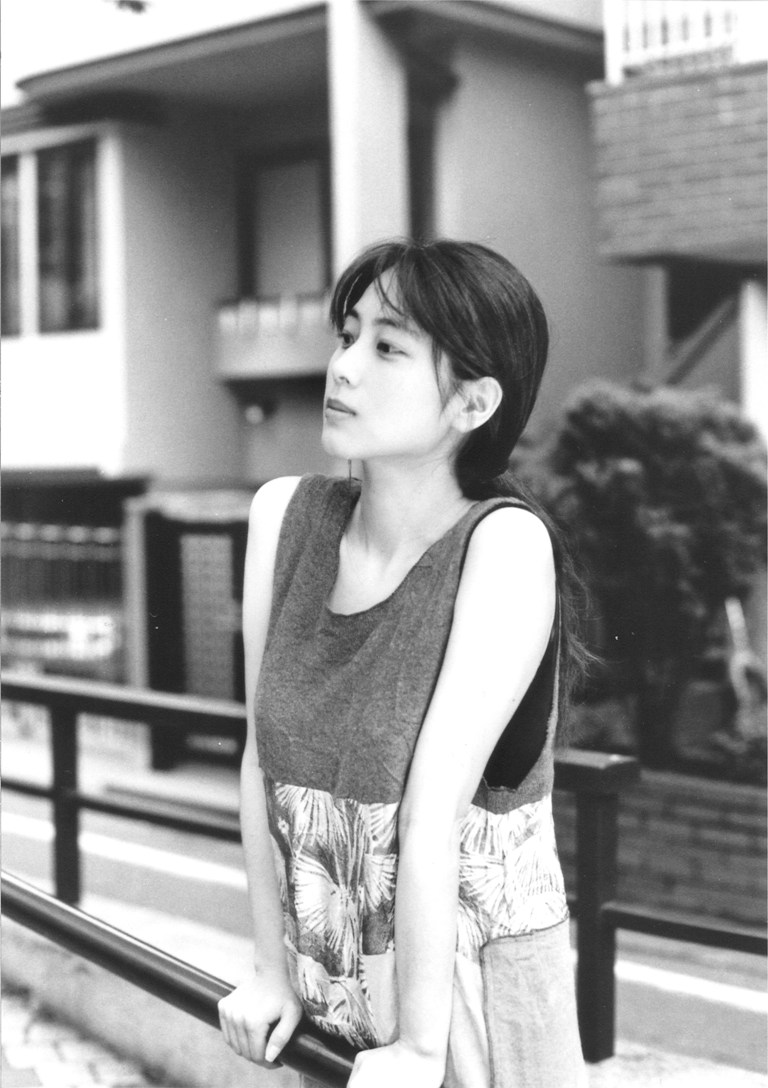
\includegraphics[width=0.6\textwidth]{P12.jpg}


\chapter{Album 4}
\thispagestyle{empty} %本页頁碼空白
\vspace{-16mm}
\LARGE {揺れる想い}

\normalsize{BGCH-1001 1993.7.10 \ release}
\\

\vspace{-5mm}

\parpic[l]{
\pichskip{6em}

\includegraphics[width=0.4\textwidth]{4.jpg}}

\small{\hyperlink{4_0}{1.揺れる想い}}

\tiny{作詞:坂井泉水 \ 作曲:織田哲郎 \ 編曲:明石昌夫}

\small{\hyperlink{4_1}{2.Season}}

\tiny{作詞:坂井泉水 \ 作曲:栗林誠一郎 \ 編曲:葉山たけし}

\small{\hyperlink{4_2}{3.君がいない}}

\tiny{作詞:坂井泉水 \ 作曲:栗林誠一郎 \ 編曲:明石昌夫}

\small{\hyperlink{4_3}{4.IN MY ARMS TONIGHT}}

\tiny{作詞:坂井泉水 \ 作曲:春畑道哉 \ 編曲:明石昌夫}

\small{\hyperlink{4_4}{5.あなたを好きだけど}}

\tiny{作詞:坂井泉水 \ 作曲:栗林誠一郎 \ 編曲:明石昌夫}

\small{\hyperlink{4_5}{6.負けないで}}

\tiny{作詞:坂井泉水 \ 作曲:織田哲郎 \ 編曲:葉山たけし}

\small{\hyperlink{4_6}{7.Listen To Me}}

\tiny{作詞:坂井泉水 \ 作曲:川島だりあ \ 編曲:明石昌夫}

\small{\hyperlink{4_7}{8.You and me (and…)}}

\tiny{作詞:坂井泉水 \ 作曲:織田哲郎 \ 編曲:葉山たけし}

\small{\hyperlink{4_8}{9.I want you}}

\tiny{作詞:坂井泉水 \ 作曲:栗林誠一郎 \ 編曲:明石昌夫}

\small{\hyperlink{4_9}{10.二人の夏}}

\tiny{作詞:坂井泉水 \ 作曲:栗林誠一郎 \ 編曲:明石昌夫}

\small{ \ }

\tiny{ \ }

\small{ \ }

\tiny{ \ }

\small{ \ }

\tiny{ \ }

\clearpage


\hypertarget{4_0}{}
\section{ 揺れる想い}

\parpic[r]{
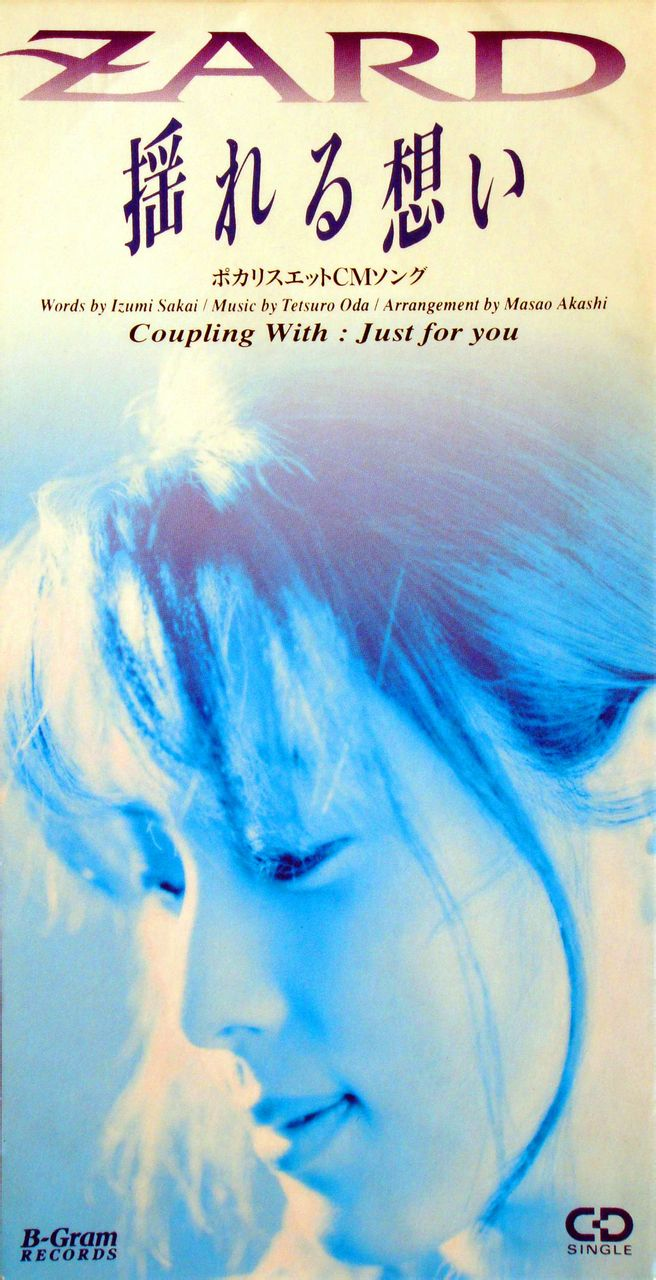
\includegraphics[width=0.3\textwidth]{S8.jpg}}

\large{

\ruby{揺}{ゆ}れる\ruby{想}{おも}い \ruby{体}{からだ}じゅう\ruby{感}{かん}じて

\ruby{君}{きみ}と\ruby{歩}{ある}き\ruby{続}{つづ}けたい  in your dream
\\

\ruby{夏}{なつ}が\ruby{忍}{しの}び\ruby{足}{あし}で  \ruby{近}{ちか}づくよ

きらめく\ruby{波}{なみ}が \ruby{砂浜}{すなはま}\ruby{潤}{うるお}して

こだわってた\ruby{周囲}{まわり}を すべて\ruby{捨}{す}てて

\ruby{今}{いま} あなたに\ruby{決}{き}めたの

こんな\ruby{自分}{じぶん}に\ruby{合}{あ}う\ruby{人}{ひと}はもう

いないと\ruby{半分}{はんぶん}あきらめてた
\\

\ruby{揺}{ゆ}れる\ruby{想}{おも}い \ruby{体}{からだ}じゅう\ruby{感}{かん}じて

このままずっとそばにいたい

\ruby{青}{あお}く\ruby{澄}{す}んだ あの\ruby{空}{そら}のような

\ruby{君}{きみ}と\ruby{歩}{ある}き\ruby{続}{つづ}けたい in your dream
\\

\ruby{好}{す}きと\ruby{合図}{あいず}\ruby{送}{おく}る \ruby{瞳}{ひとみ}の\ruby{奥}{おく}

\ruby{覗}{のぞ}いてみる\ruby{振}{ふ}りして キスをした

すべてを\ruby{見}{み}せるのが \ruby{怖}{こわ}いから

やさしさから\ruby{逃}{に}げてたの

\ruby{運命}{うんめい}の\ruby{出逢}{であ}い \ruby{確}{たし}かね こんなに

\ruby{自分}{じぶん}が \ruby{変}{か}わってくなんて
\\

\ruby{揺}{ゆ}れる\ruby{想}{おも}い \ruby{体}{からだ}じゅう\ruby{感}{かん}じて

このままずっとそばにいたい

いくつ\ruby{淋}{さび}しい\ruby{季節}{きせつ}が\ruby{来}{き}ても

ときめき \ruby{抱}{だ}きしめていたい in my dream
\\

\ruby{揺}{ゆ}れる\ruby{想}{おも}い \ruby{体}{からだ}じゅう\ruby{感}{かん}じて

このままずっとそばにいたい

\ruby{青}{あお}く\ruby{澄}{す}んだ あの\ruby{空}{そら}のような

\ruby{君}{きみ}と\ruby{歩}{ある}き\ruby{続}{つづ}けたい in your dream

}

\hypertarget{4_1}{}
\section{ season}
\large{

\ruby{ポプラ}{poplar}の\ruby{並木}{なみき}をくすぐる

\ruby{風}{かぜ}は\ruby{春色}{はるいろ}きらめいているね

あの\ruby{日}{ひ}と\ruby{同}{おな}じ\ruby{道}{みち}\ruby{行}{い}く\ruby{制服}{せいふく}\ruby{達}{たち}

ふと\ruby{懷}{なつ}かしく\ruby{胸}{むね}に\ruby{藍}{あお}い\ruby{時間}{とき}
\\

\ruby{切}{せつ}なくて \ruby{出}{だ}しそびれた\ruby{手紙}{てがみ}

いつも\ruby{遠}{とお}くから\ruby{君}{きみ}を\ruby{思}{おも}い oh

\ruby{言}{い}えなくて \ruby{惱}{なや}んでいた あのseason

いつの\ruby{日}{ひ}か \ruby{卒業}{そつぎょう}したね
\\

\ruby{記念}{きねん}の\ruby{アルバム}{album} \ruby{今}{いま}でも

\ruby{時々}{ときどき}は\ruby{開}{ひら}いて\ruby{見}{み}るけど

\ruby{薄}{うす}れゆく \ruby{君}{きみ}への\ruby{憧}{あこが}れに

\ruby{青春}{せいしゅん}の\ruby{意味}{いみ}を\ruby{知}{し}らされた
\\

\ruby{切}{せつ}なくて \ruby{淡}{あわ}い\ruby{夢}{ゆめ}を\ruby{抱}{だ}き

\ruby{輝}{かがや}いた\ruby{景色}{けしき}には \ruby{帰}{かえ}れない oh

\ruby{言}{い}えなくて \ruby{唇}{くちびる}\ruby{咬}{か}んだ season

いつの\ruby{日}{ひ}か \ruby{卒業}{そつぎょう}したね
\\

\ruby{切}{せつ}なくて \ruby{出}{だ}しそびれた\ruby{手紙}{てがみ}

いつも\ruby{遠}{とお}くから\ruby{君}{きみ}を\ruby{思}{おも}い oh

\ruby{言}{い}えなくて \ruby{惱}{なや}んでいた あのseason

いつの\ruby{日}{ひ}か \ruby{卒業}{そつぎょう}したね
\\

いつの\ruby{日}{ひ}か \ruby{卒業}{そつぎょう}したね
\\

I'll remember you and windy season

}

\hypertarget{4_2}{}
\section{ 君がいない (B-version)}
\large{

\ruby{君}{きみ}がいない

あの\ruby{頃}{ころ}の\ruby{二人}{ふたり}も \ruby{今}{いま}はいない
\\

\ruby{本当}{ほんとう}は \ruby{少}{すこ}しだけ\ruby{悔}{く}やんでるわ

\ruby{何故}{なぜ}なの? \ruby{君}{きみ}に\ruby{出会}{であ}い fall in love

\ruby{無口}{むぐち}でも そんなとこ\ruby{好}{す}きだったのに

\ruby{君}{き}が\ruby{嘘}{うそ}をつくなんてね

ときめきが やすらぎに\ruby{変}{か}われば

\ruby{刺激}{しげき}という \ruby{スパイス}{spice}だって\ruby{必要}{ひつよう}かもね
\\

\ruby{君}{きみ}がいない

やさしかった\ruby{君}{きみ} \ruby{今}{いま}はいない
\\

\parpic[r]{
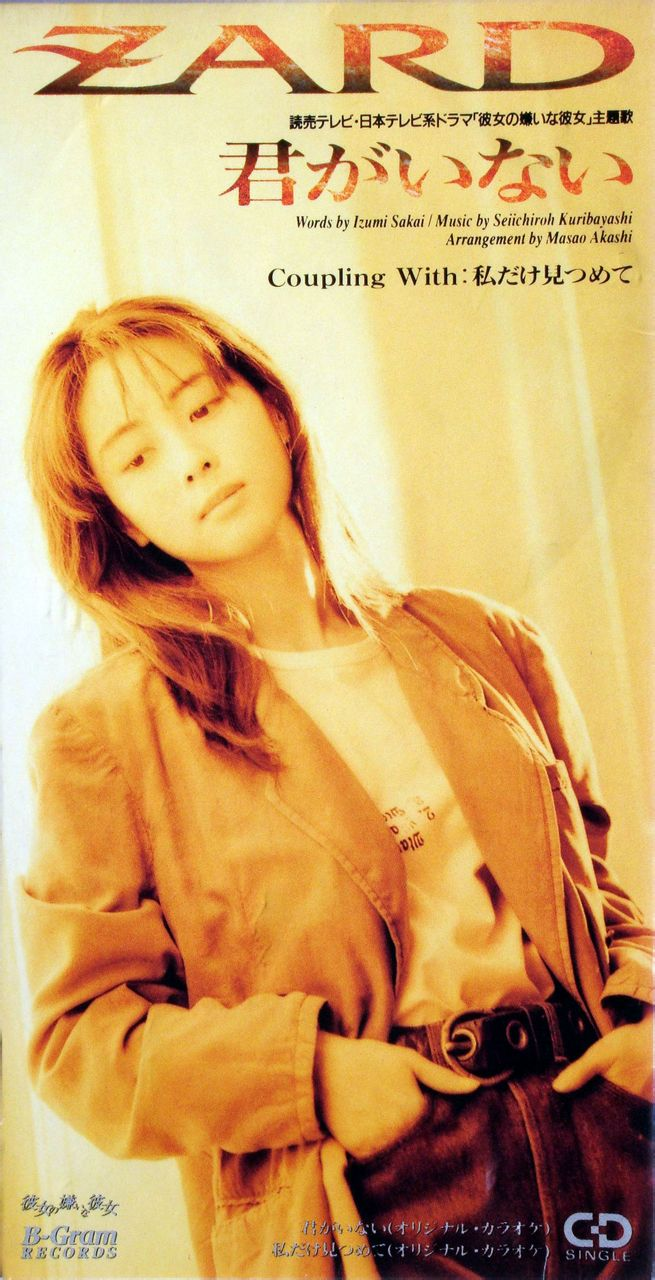
\includegraphics[width=0.3\textwidth]{S7.jpg}}

よく\ruby{行}{い}った \ruby{海岸}{かいがん}\ruby{沿}{ぞ}いの\ruby{店}{みせ}を

\ruby{通}{とお}るたび \ruby{少}{すこ}し\ruby{胸}{むね}が\ruby{痛}{いた}い

\ruby{逃}{に}げてゆく\ruby{幸}{しあわ}せに\ruby{気}{き}づいた\ruby{時}{とき}

\ruby{人}{ひと}は“もう\ruby{戻}{もど}れない”と\ruby{思}{おも}うの

やりきれない\ruby{週末}{しゅうまつ}の\ruby{メニュー}{menu}は

\ruby{思}{おも}い\ruby{出}{で}を\ruby{整理}{かたづけ}たり \ruby{映画}{えいが}を\ruby{見}{み}たり
\\

\ruby{君}{きみ}がいない

あの\ruby{頃}{ころ}の\ruby{二人}{ふたり}も \ruby{今}{いま}はいない

\ruby{何}{なに}もかも \ruby{時間}{とき}のすれ\ruby{違}{ちが}いと

\ruby{感}{かん}じた その\ruby{時}{とき} \ruby{切}{せつ}なく good-bye
\\

\ruby{君}{きみ}がいない

あの\ruby{頃}{ころ}の\ruby{二人}{ふたり}も \ruby{今}{いま}はいない

\ruby{何}{なに}もかも \ruby{時間}{とき}のすれ\ruby{違}{ちが}いと

\ruby{感}{かん}じた その\ruby{時}{とき} \ruby{切}{せつ}なく good-bye

}

\hypertarget{4_3}{}
\section{ In my arms tonight}
\large{

そう\ruby{知}{し}らなかった \ruby{今}{いま}も\ruby{愛}{あい}してるなんて

\ruby{雨}{あめ}の\ruby{降}{ふ}る\ruby{日}{ひ}は\ruby{切}{せつ}ない

いつも\ruby{忘}{わす}れないでいるわ そう あなたのことだけ

たまには\ruby{束縛}{そくばく}して my love
\\

\ruby{声}{こえ}を\ruby{聴}{き}かせて \ruby{熱}{あつ}く\ruby{見}{み}つめて

あの\ruby{頃}{ころ}のように

\ruby{季節}{きせつ}も\ruby{街}{まち}も \ruby{流}{なが}れてく

\ruby{夢}{ゆめ}を\ruby{見}{み}させて \ruby{時間}{じかん}を\ruby{止}{と}めて

ねえ \ruby{少年}{しょうねん}のように\ruby{甘}{あま}えてほしい

Let me hold you in my arms tonight
\\

\ruby{誤解}{ごかい}で\ruby{始}{はじ}まったけど \ruby{不器用}{ぶきよう}な\ruby{二人}{ふたり}

\ruby{今}{いま}なら\ruby{痛}{いた}みもわかる

いつも\ruby{強}{つよ}がっていたの あなた\ruby{困}{こま}らせたくて

\ruby{夏}{なつ}の\ruby{日}{ひ}に\ruby{帰}{かえ}りたい my love
\\

\ruby{声}{こえ}を\ruby{聴}{き}かせて \ruby{熱}{あつ}く\ruby{見}{み}つめて

\ruby{揺}{ゆ}れる\ruby{心}{こころ}に

\ruby{秋}{あき}の\ruby{気配}{けはい}が \ruby{近}{ちか}づくわ

\ruby{夢}{ゆめ}を\ruby{見}{み}させて \ruby{時間}{じかん}を\ruby{止}{と}めて

ひとり\ruby{占}{じ}めしたいの わかってほしい

Let me hold you in my arms tonight
\\

\ruby{声}{こえ}を\ruby{聴}{き}かせて \ruby{熱}{あつ}く\ruby{見}{み}つめて

あの\ruby{頃}{ころ}のように

\ruby{季節}{きせつ}も\ruby{街}{まち}も \ruby{流}{なが}れてく

\ruby{夢}{ゆめ}を\ruby{見}{み}させて \ruby{時間}{じかん}を\ruby{止}{と}めて

ねえ \ruby{少年}{しょうねん}のように\ruby{甘}{あま}えてほしい

Let me hold you in my arms tonight

}
{ \ }


\includegraphics[width=0.5\textwidth]{S5.jpg}

\hypertarget{4_4}{}
\section{ あなたを好きだけど}
\large{

\ruby{眠}{ねむ}そうな\ruby{新聞}{しんぶん}\ruby{記事}{きじ}で

いつも\ruby{朝}{あさ}が\ruby{始}{はじ}まる

どなりにいる\ruby{彼}{かれ}は\ruby{年下}{としした}

ニクメない\ruby{笑顔}{えがお}が\ruby{トレードマーク}{trademark}

ものわかりのイイ\ruby{女}{おんな}

でも\ruby{本当}{ほんとう}は\ruby{私}{わたし}

すごく\ruby{心配性}{しんぱいしょう}なの
\\

あなたを\ruby{好}{す}きだけど…

\ruby{時々}{ときどき}つらいの

その\ruby{若}{わか}さ\ruby{眩}{まぶ}しすぎるから

あなたが\ruby{好}{す}きだけど…

\ruby{悲}{かな}しくなるの

たまには\ruby{甘}{あま}えさせて
\\

あなたは\ruby{調子}{ちょうし}\ruby{外}{はず}れの

\ruby{歌}{うた}をうたい \ruby{着変}{きが}える

\ruby{髪型}{かみがた}だって \ruby{変}{か}わらない\ruby{私}{わたし}

\ruby{同}{おな}じ\ruby{気持}{きも}ちでいるのに

もしも\ruby{年上}{としうえ}の\ruby{男性}{ひと}が\ruby{現}{あらわ}れたら

\ruby{揺}{ゆ}れてしまいそう やさしさに
\\

あなたが\ruby{好}{す}きだけど…

\ruby{時々}{ときどき}つらいの

あまりに\ruby{正直}{しょうじき}すぎるから

あなたが\ruby{好}{す}きだけど…

\ruby{少}{すこ}しコワイの

\ruby{言葉}{ことば}にすればフェイドアウト
\\

あなたが\ruby{好}{す}きだけど…

\ruby{時々}{ときどき}つらいの

あまりに\ruby{正直}{しょうじき}すぎるから

あなたが\ruby{好}{す}きだけど…

\ruby{少}{すこ}しコワイの

\ruby{言葉}{ことば}にすればフェイドアウト

}

\hypertarget{4_5}{}
\section{ 負けないで}

\large{

ふとした\ruby{瞬間}{しゅんかん}に \ruby{視線}{しせん}がぶつかる

\ruby{幸運}{しあわせ}のときめき  \ruby{覚}{おぼ}えているでしょ

\ruby{パステルカラー}{Pastel Color}の\ruby{季節}{きせず}に\ruby{恋}{こい}した

あの\ruby{日}{ひ}のように \ruby{輝}{かがや}いてる あなたでいてね
\\

\ruby{負}{ま}けないで もう\ruby{少}{すこ}し

\ruby{最後}{さいご}まで \ruby{走}{はし}り\ruby{抜}{ぬ}けて

どんなに \ruby{離}{はな}れてても

\ruby{心}{こころ}は そばにいるわ

\ruby{追}{お}いかけて \ruby{遥}{はる}かな\ruby{夢}{ゆめ}を
\\

\ruby{何}{なに}が\ruby{起}{お}きたって ヘッチャラな\ruby{顔}{かお}して

どうにかなるサと おどけてみせるの

「\ruby{今宵}{こよい}は\ruby{私}{わたくし}と\ruby{一緒}{いっしょ}に\ruby{踊}{おど}りましょ」

\ruby{今}{いま}も そんなあなたが\ruby{好}{す}きよ \ruby{忘}{わす}れないで
\\

\parpic[r]{
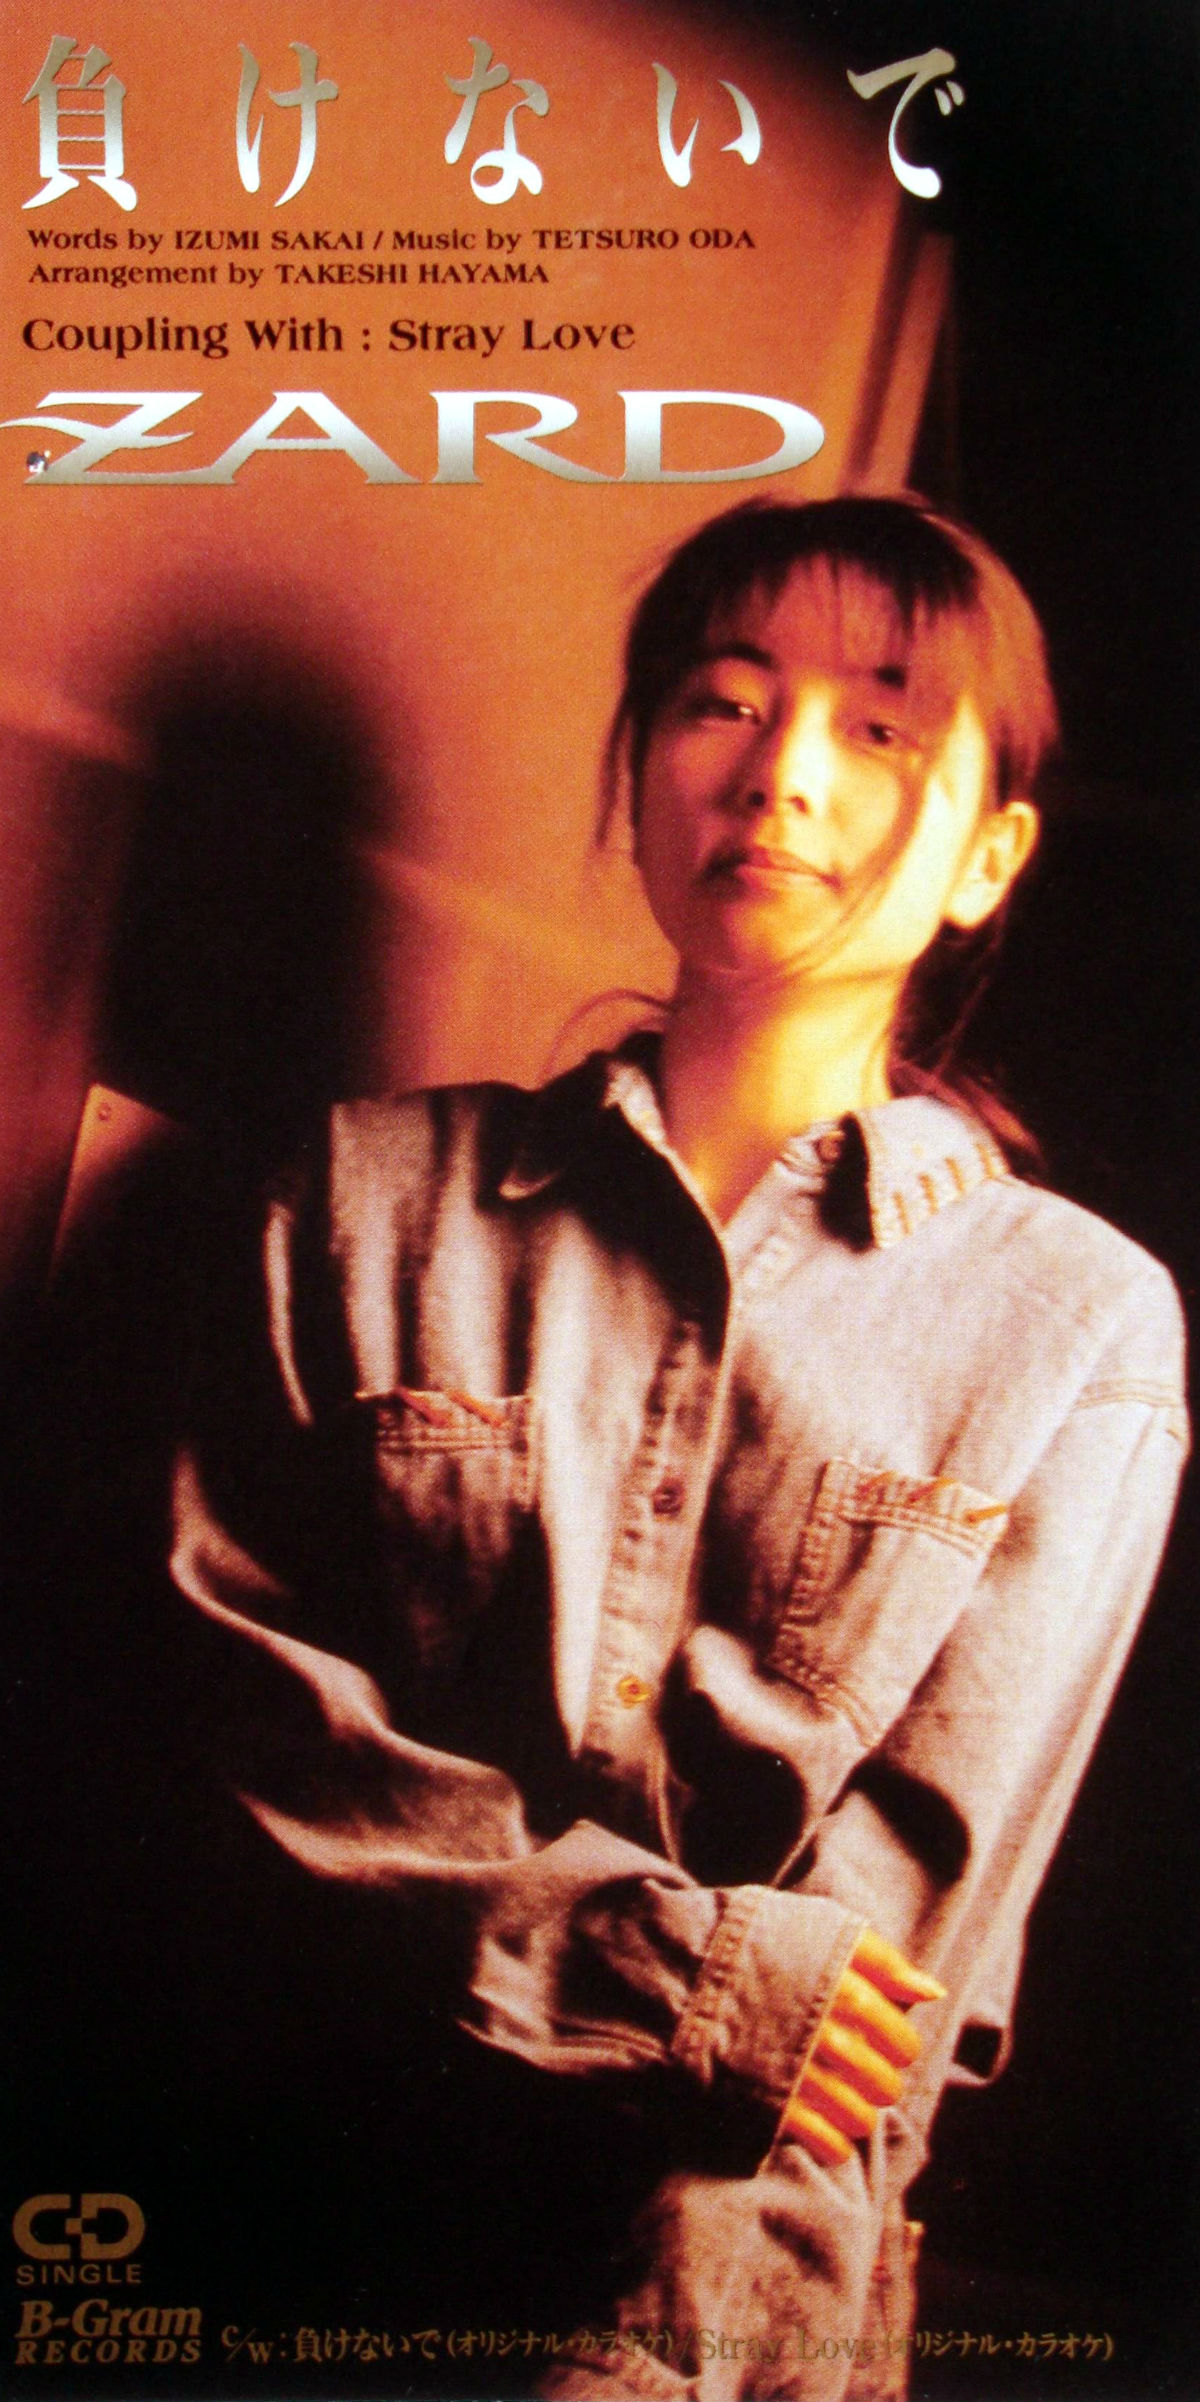
\includegraphics[width=0.3\textwidth]{S6.jpg}}

\ruby{負}{ま}けないで ほらそこに

\ruby{ゴール}{Goal}は\ruby{近}{ちか}づいてる

どんなに \ruby{離}{はな}れてても

\ruby{心}{こころ}は そばにいるわ

\ruby{感}{かん}じてね \ruby{見}{み}つめる\ruby{瞳}{ひとみ}
\\

\ruby{負}{ま}けないで もう\ruby{少}{すこ}し

\ruby{最後}{さいご}まで \ruby{走}{はし}り\ruby{抜}{ぬ}けて

どんなに \ruby{離}{はな}れてても

\ruby{心}{こころ}は そばにいるわ

\ruby{追}{お}いかけて \ruby{遥}{はる}かな\ruby{夢}{ゆめ}を
\\

\ruby{負}{ま}けないで ほらそこに

\ruby{ゴール}{Goal}は\ruby{近}{ちか}づいてる

どんなに \ruby{離}{はな}れてても

\ruby{心}{こころ}は そばにいるわ

\ruby{感}{かん}じてね \ruby{見}{み}つめる\ruby{瞳}{ひとみ}

}

\hypertarget{4_6}{}
\section{ Listen to me}
\large{

つらい\ruby{朝}{あさ}は \ruby{好}{す}きな\ruby{曲}{きょく}も

\ruby{目覚}{めざ}ましにならない

\ruby{軽}{かる}い\ruby{ブレックファースト}{brack fast}\ruby{流}{なが}しこんで

\ruby{地下鉄}{ちかてつ}まで Hurry Up

イヤになっちゃう \ruby{満員}{まんいん}\ruby{電車}{でんしゃ}は Biggest Zoo

\ruby{乙女}{おとめ}\ruby{心}{ごころ}の \ruby{髪}{かみ}も \ruby{靴}{くつ}もダイナシよ

\ruby{夢}{ゆめ}も\ruby{恋}{こい}も\ruby{遠}{とお}いなんで

\ruby{淋}{さび}しいじゃない
\\

Listen to me くり\ruby{出}{だ}そう

\ruby{巨大}{きょだい}な\ruby{ビル}{bill}の\ruby{迷路}{めいろ}なんか\ruby{怖}{こわ}くない

We'll be all right ありふれた\ruby{日常}{にちじょう}の

\ruby{キャパシティー}{capacity}\ruby{越}{こ}えなくちゃね
\\

\ruby{人}{ひと}のうわさ うんざりする

かしましい Tea time

\ruby{嫌}{きら}いな \ruby{ユニフォーム}{uniform}

\ruby{少}{すこ}し\ruby{ヒップ}{VIP} \ruby{太}{ふと}ったみたい Oh my God!

ホンネとタテマエ

\ruby{段々}{だんだん}\ruby{大人}{おとな}になってる\ruby{証拠}{しょうこ}

\ruby{忘}{わす}れたくない \ruby{ハート}{heart}は\ruby{ソウル}{soul}

つまずいても \ruby{傷}{きず}ついても

\ruby{愛}{あい}があれば \ruby{楽}{たの}しいじゃない
\\

Listen to me \ruby{飛}{と}び\ruby{出}{だ}そう

\ruby{ダークグレー}{dark gray} \ruby{空}{そら}の\ruby{色}{いろ} \ruby{塗}{ぬ}り\ruby{変}{か}え

We'll be all right, never give it up!

\ruby{每朝}{まいあさ}が\ruby{新}{あたら}しい \ruby{ページ}{page}の\ruby{始}{はじ}まり
\\

Listen to me くり\ruby{出}{だ}そう

\ruby{巨大}{きょだい}な\ruby{ビル}{bill}の\ruby{迷路}{めいろ}なんか\ruby{怖}{こわ}くない

We'll be all right ありふれた\ruby{日常}{にちじょう}の

\ruby{キャパシティー}{capacity}\ruby{越}{こ}えなくちゃね
\\

Listen to me \ruby{飛}{と}び\ruby{出}{だ}そう

\ruby{ダークグレー}{dark gray} \ruby{空}{そら}の\ruby{色}{いろ} \ruby{塗}{ぬ}り\ruby{変}{か}え

We'll be all right, never give it up!

\ruby{每朝}{まいあさ}が\ruby{新}{あたら}しい \ruby{ページ}{page}の\ruby{始}{はじ}まり

}

\hypertarget{4_7}{}
\section{ You and me(and...)}
\large{

「\ruby{街路樹}{がいろじゅ}の\ruby{下}{した}で\ruby{約束}{やくそく}した」と

\ruby{彼女}{かのじょ}のはずむ\ruby{声}{こえ}に\ruby{私}{わたし}

\ruby{戸惑}{とまど}いを\ruby{隠}{かく}せなかった

\ruby{イヴ}{eve}の\ruby{夜}{よる}はたぶん

\ruby{彼女}{かのじょ}と\ruby{過}{す}ごすのね
\\

もう\ruby{出來}{でき}ないわ \ruby{演}{えん}じられない

\ruby{屆}{とど}かない\ruby{想}{おも}いはただ

\ruby{粉雪}{こなゆき}が\ruby{舞}{ま}う\ruby{街}{まち}に\ruby{消}{き}えてゆく

\ruby{崩}{くず}れ\ruby{始}{はじ}めた\ruby{ハーモニー}{harmony}

You and me
\\

「\ruby{今}{いま}だけ\ruby{考}{かんが}えて」そう\ruby{言}{い}って\ruby{抱}{だ}いた

\ruby{感}{かん}じてるのに\ruby{胸}{むね}が\ruby{痛}{いた}い

\ruby{許}{ゆる}されぬ\ruby{夢}{ゆめ}を\ruby{見}{み}たの

\ruby{彼女}{かのじょ}と\ruby{友達}{ともだち}でいたいの これからも
\\

もう\ruby{泣}{な}かないで \ruby{愛}{あい}は\ruby{殘酷}{ざんこく}ね

あたためた\ruby{時間}{とき}は\ruby{遠}{とお}い

\ruby{出逢}{であ}った\ruby{頃}{ころ}にもう\ruby{戾}{もど}れないの

\ruby{風}{かぜ}に\ruby{途切}{とぎ}れた\ruby{ハーモニー}{harmony}

You and me
\\

もう\ruby{出來}{でき}ないわ \ruby{演}{えん}じられない

\ruby{屆}{とど}かない\ruby{想}{おも}いはただ

\ruby{粉雪}{こなゆき}が\ruby{舞}{ま}う\ruby{街}{まち}に\ruby{消}{き}えてゆく

\ruby{崩}{くず}れ\ruby{始}{はじ}めた\ruby{ハーモニー}{harmony}

You and me
\\

もう\ruby{泣}{な}かないで \ruby{愛}{あい}は\ruby{殘酷}{ざんこく}ね

あたためた\ruby{時間}{とき}は\ruby{遠}{とお}い

\ruby{出逢}{であ}った\ruby{頃}{ころ}にもう\ruby{戾}{もど}れないの

\ruby{風}{かぜ}に\ruby{途切}{とぎ}れた\ruby{ハーモニー}{harmony}

You and me

}

\hypertarget{4_8}{}
\section{ I want you}
\large{

この\ruby{頃}{ごろ}お\ruby{互}{たが}い\ruby{話題}{わだい}\ruby{不足}{ふそく}ね \ruby{会}{あ}·い·す·ぎ?

\ruby{去年}{きょねん}の\ruby{夏}{なつ}にくれた\ruby{イヤリング}{earring}

\ruby{今日}{きょう}もしているのに

あなたは\ruby{気}{き}に\ruby{止}{と}めず

\ruby{月}{つき}を\ruby{追}{お}いかけ Driving

\ruby{五月}{ごがつ}の\ruby{街}{まち}も \ruby{色}{いろ}あせて\ruby{見}{み}える

もっと\ruby{リアル}{real}に \ruby{愛}{あい}し\ruby{合}{あ}えたら
\\

I want you

あなたの\ruby{声}{こえ}が\ruby{聴}{き}こえる Midnight

はなれてると\ruby{熱}{あつ}く\ruby{燃}{も}える My heart

さめた\ruby{身体}{からだ}に\ruby{情熱}{じょうねつ}\ruby{注}{そそ}いで

この\ruby{現実}{げんじつ}\ruby{壊}{こわ}したいわ My life
\\

\ruby{煙草}{タバコ}を\ruby{吸}{す}う\ruby{仕草}{しぐさ}

\ruby{誰}{だれ}かに\ruby{似}{に}ていて\ruby{好}{す}きなの

\ruby{息}{いき}を\ruby{殺}{ころ}して\ruby{部屋}{へや}で\ruby{見}{み}た Movie

\ruby{二人}{ふたり}だけのひととき

あなたを\ruby{知}{し}る\ruby{程}{ほど}に

すべての\ruby{好}{この}みが\ruby{変}{か}わった

“おまえらしくない”なんて…

もっと\ruby{オープン}{open}に\ruby{付}{つ}き\ruby{合}{あ}いたい
\\

I want you

\ruby{私}{わたし}の\ruby{声}{こえ}を\ruby{感}{かん}じて Midnight

\ruby{瞳}{ひとみ}\ruby{閉}{と}じれば\ruby{震}{ふ}える My body

ラ ラ ラ ラ ラ…

この\ruby{現実}{げんじつ}\ruby{壊}{こわ}したいわ My love
\\

I want you

あなたの\ruby{声}{こえ}が\ruby{聴}{き}こえる Midnight

はなれてると\ruby{熱}{あつ}く\ruby{燃}{も}える My heart

ラ ラ ラ ラ ラ…

この\ruby{現実}{げんじつ}\ruby{壊}{こわ}したいわ My life

}

\hypertarget{4_9}{}
\section{ 二人の夏}
\large{

\ruby{偶然}{ぐうぜん}に\ruby{見}{み}かけたの \ruby{バス}{bus}\ruby{停}{てい}で

\ruby{結婚}{けっこん}するとうわさで\ruby{聞}{き}いたけど

\ruby{スーツ}{suit}\ruby{姿}{すがた}のあなたは

やけに\ruby{大人}{おとな}に\ruby{見}{み}えた

\ruby{少}{すこ}し\ruby{距離}{きょり}\ruby{感}{かん}じたせい?

\ruby{声}{こえ}かけそびれたの
\\

わすれかけた \ruby{二人}{ふたり}の\ruby{夏}{なつ}

\ruby{胸}{むね}に\ruby{甦}{よみがえ}る

あれからもう どれくらいの\ruby{月日}{とき}が\ruby{過}{た}ったのだろう

\ruby{振}{ふ}り\ruby{向}{む}くはずのないあなたに

サヨナラ\ruby{言}{い}った

どうかずっと\ruby{変}{か}わらずにいて

\ruby{大好}{だいす}きだった \ruby{笑顔}{えがお}だけは
\\

\ruby{別離}{わかれ}でも しばらくは\ruby{悲}{かな}しくて

あなたの\ruby{電話}{でんわ} ずっと\ruby{待}{ま}っていたの

\ruby{今}{いま}はもうそれぞれに\ruby{違}{ちが}う\ruby{パートナー}{partner}\ruby{見}{み}つけ

\ruby{別}{べつ}の\ruby{道}{みち}\ruby{歩}{ある}き\ruby{出}{だ}した

もう\ruby{戻}{もど}らないわ
\\

\ruby{輝}{かがや}いてた \ruby{二人}{ふたり}の\ruby{夏}{なつ}

\ruby{波}{なみ}がさらうように

いつかはきっと\ruby{遠}{とお}い\ruby{記憶}{きおく}の\ruby{彼方}{かなた}に\ruby{消}{き}えてく

あなたの\ruby{写真}{しゃしん}\ruby{大切}{たいせつ}にしまっておくわ

いつかどこかでまた\ruby{逢}{あ}えるこど

\ruby{祈}{いの}ってるわ \ruby{元気}{げんき}でね…

}


\chapter{Album 5}
\thispagestyle{empty} %本页頁碼空白
\vspace{-16mm}
\LARGE {OH MY LOVE}

\normalsize{BGCH-1014 1994.6.4 \ release}
\\

\vspace{-5mm}

\parpic[l]{
\pichskip{6em}

\includegraphics[width=0.4\textwidth]{5.jpg}}

\small{\hyperlink{5_0}{1.Oh my love}}

\tiny{作詞:坂井泉水 \ 作曲:織田哲郎 \ 編曲:明石昌夫}

\small{\hyperlink{5_1}{2.Top Secret}}

\tiny{作詞:坂井泉水 \ 作曲:栗林誠一郎 \ 編曲:明石昌夫}

\small{\hyperlink{5_2}{3.きっと忘れない}}

\tiny{作詞:坂井泉水 \ 作曲:織田哲郎 \ 編曲:明石昌夫}

\small{\hyperlink{5_3}{4.もう少し あと少し…}}

\tiny{作詞:坂井泉水 \ 作曲:栗林誠一郎 \ 編曲:明石昌夫}

\small{\hyperlink{5_4}{5.雨に濡れて}}

\tiny{作詞:坂井泉水/上杉昇 \ 作曲:栗林誠一郎 \ 編曲:明石昌夫}

\small{\hyperlink{5_5}{6.この愛に泳ぎ疲れても}}

\tiny{作詞:坂井泉水 \ 作曲:織田哲郎 \ 編曲:明石昌夫}

\small{\hyperlink{5_6}{7.I still remember}}

\tiny{作詞:坂井泉水 \ 作曲:栗林誠一郎 \ 編曲:明石昌夫}

\small{\hyperlink{5_7}{8.If you gimme smile}}

\tiny{作詞:坂井泉水 \ 作曲:栗林誠一郎 \ 編曲:明石昌夫}

\small{\hyperlink{5_8}{9.来年の夏も}}

\tiny{作詞:坂井泉水 \ 作曲:栗林誠一郎 \ 編曲:明石昌夫}

\small{\hyperlink{5_9}{10.あなたに帰りたい}}

\tiny{作詞:坂井泉水 \ 作曲:栗林誠一郎 \ 編曲:明石昌夫}

\small{ \ }

\tiny{ \ }

\small{ \ }

\tiny{ \ }

\small{ \ }

\tiny{ \ }

\clearpage


\hypertarget{5_0}{}
\section{ OH MY LOVE}
\large{

ゆるい\ruby{坂道}{さかみち} \ruby{自転車}{じてんしゃ}\ruby{押}{お}しながら

\ruby{家}{いえ}まで\ruby{送}{おく}ってくれた

あなたは \ruby{私}{わたし}の\ruby{名前}{なまえ}\ruby{呼}{よ}び\ruby{捨}{す}てにして

\ruby{夕暮}{ゆぐ}れに\ruby{微笑}{ほほえ}んでいたけど
\\

ほら \ruby{加}{か}\ruby{速度}{そくど}つけて

あなたを\ruby{好}{す}きになる

Oh my love

もう\ruby{友達}{ともだち}の\ruby{エリア}{Area}はみ\ruby{出}{だ}した

\ruby{一緒}{いっしょ}にいる\ruby{時}{とき}の

\ruby{自分}{じぶん}が\ruby{一番}{いちばん}\ruby{好}{す}き

\ruby{週末}{しゅうまつ}まで\ruby{待}{ま}ち\ruby{切}{き}れない

そんな\ruby{胸}{むな}さわぎ \ruby{揺}{ゆ}れる\ruby{午後}{ごご}
\\

うつ\ruby{向}{む}く\ruby{横}{よこ}\ruby{顔}{がお} \ruby{何}{なに}か\ruby{悩}{なや}んでるの?

その\ruby{理由}{わけ}を\ruby{教}{おし}えて

\ruby{初}{はじ}めての\ruby{キス}{Kiss}の\ruby{日}{ひ} \ruby{街}{まち}は

\ruby{スローモーション}{Slow Motion}に

\ruby{交差}{こうさ}する\ruby{クラクション}{Klaxon}で\ruby{夢}{ゆめ}が\ruby{覚}{さ}めた
\\

ほら \ruby{走}{はし}り\ruby{出}{だ}したわ

あなたへの\ruby{プロローグ}{Prologue}

Oh my love

\ruby{無}{む}\ruby{意識}{いしき}に\ruby{髪}{かみ}をのばし\ruby{始}{はじ}めたの

あなたといる\ruby{時}{とき}の

\ruby{素直}{すなお}な\ruby{自分}{じぶん}が\ruby{好}{す}き

\ruby{私}{わたし}の\ruby{存在}{そんざい}どれくらい?

\ruby{広}{ひろ}い\ruby{背}{せ}\ruby{中}{なか}に\ruby{問}{と}いかける\ruby{夏}{なつ}
\\

ほら \ruby{加}{か}\ruby{速度}{そくど}つけて

あなたを\ruby{好}{す}きになる

Oh my love

もう\ruby{友達}{ともだち}の\ruby{エリア}{Area}はみ\ruby{出}{だ}した

\ruby{一緒}{いっしょ}にいる\ruby{時}{とき}の

\ruby{自分}{じぶん}が\ruby{一番}{いちばん}\ruby{好}{す}き

\ruby{週末}{しゅうまつ}まで\ruby{待}{ま}ち\ruby{切}{き}れない

そんな\ruby{胸}{むな}さわぎ \ruby{揺}{ゆ}れる\ruby{午後}{ごご}
\\

あなたといる\ruby{時}{とき}の

\ruby{素直}{すなお}な\ruby{自分}{じぶん}が\ruby{好}{す}き

\ruby{私}{わたし}の\ruby{存在}{そんざい}どれくらい?

\ruby{広}{ひろ}い\ruby{背}{せ}\ruby{中}{なか}に\ruby{問}{と}いかける\ruby{夏}{なつ}

}

\hypertarget{5_1}{}
\section{ Top Secret}
\large{

\ruby{今夜}{こんや}の\ruby{シチュー}{stew} \ruby{自信}{じしん}あったのに

「\ruby{遲}{おそ}くなるから…」 なんてヒドイ!

もっと\ruby{一緖}{いっしょ}に\ruby{居}{い}られると\ruby{思}{おも}ってた

\ruby{暮}{く}らし\ruby{始}{はじ}めた\ruby{頃}{ころ}は
\\

\ruby{街}{まち}を\ruby{歩}{ある}けば \ruby{素敵}{すてき}な\ruby{誘惑}{ゆうわく}

It's my top secret わかってない

\ruby{女}{おんな}の\ruby{子}{こ}ってね \ruby{自分}{じぶん}のやる\ruby{事}{こと}に

\ruby{線引}{せんひ}いたり \ruby{決}{き}めたり
\\

\ruby{今日}{きょう} \ruby{昔}{むかし}の\ruby{彼}{かれ}に\ruby{電話}{でんわ}しちゃったわ

ドキドキ \ruby{壞}{こわ}れそうな\ruby{ハート}{heart} \ruby{懷}{なつ}かしい

あなたとは\ruby{違}{ちが}う \ruby{彼}{かれ}の\ruby{性格}{せいかく}は

\ruby{全然}{ぜんぜん}\ruby{変}{か}わってなかったけど

やっばりね あなたの\ruby{方}{ほう}がイイ
\\

\ruby{最初}{さいしょ}\ruby{友達}{みんな}が\ruby{反対}{はんたい}してたの

It's my top secret うわさ\ruby{聞}{き}いて

けんかするほと \ruby{仲}{なか}のいいそこだって

\ruby{ワイドショー}{wide show}にもならない
\\

いつ \ruby{二人}{ふたり}で\ruby{愛}{あい}を\ruby{確}{たし}かめ\ruby{合}{あ}うのよ

ときどき \ruby{魅力}{みりょく}ないのかなって\ruby{鏡}{かがみ}のぞく

\ruby{スープ}{soup}の\ruby{冷}{さ}めないうち \ruby{笑顔}{えがお}を\ruby{見}{み}せてね

トゥルルル \ruby{コール}{call}\ruby{5回}{ごかい}\ruby{鳴}{なって}って

ちょっとイヤな\ruby{予感}{よかん}がしたけど
\\

\ruby{今日}{きょう} \ruby{昔}{むかし}の\ruby{彼}{かれ}に\ruby{電話}{でんわ}しちゃったわ

ドキドキ \ruby{壞}{こわ}れそうな\ruby{ハート}{heart} \ruby{懷}{なつ}かしい

あなたとは\ruby{違}{ちが}う \ruby{彼}{かれ}の\ruby{性格}{せいかく}は

\ruby{全然}{ぜんぜん}\ruby{変}{か}わってなかったけど

やっばりね あなたの\ruby{方}{ほう}がイイ

}

\hypertarget{5_2}{}
\section{ きっと忘れない}

\parpic[r]{
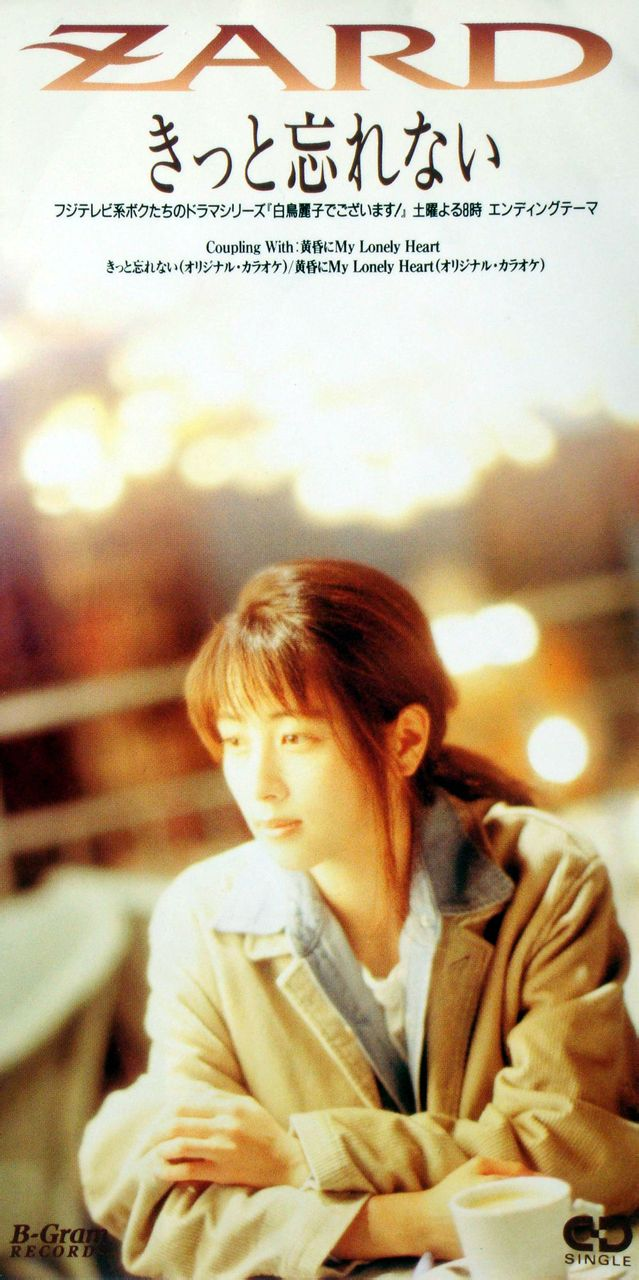
\includegraphics[width=0.3\textwidth]{S10.jpg}}

\large{

きっと\ruby{忘}{わす}れない \ruby{眩}{まぶ}しいまなざしを

\ruby{信}{しん}じたい \ruby{信}{しん}じてる

あなたが\ruby{変}{か}わらぬように
\\

every day  every night \ruby{泣}{な}いたりしたけど

\ruby{誰}{だれ}にも\ruby{話}{はな}せなくて

\ruby{無器用}{ぶきよう}だけど せいいっぱいあなたを

\ruby{愛}{あい}した あの\ruby{季節}{きせつ}

\ruby{暮}{く}れゆく\ruby{都会}{まち} あふれる\ruby{人波}{ひとなみ}

\ruby{今}{いま}にも\ruby{笑顔}{えがお}であなたが\ruby{現}{あらわ}れそうで
\\

きっと\ruby{忘}{わす}れない また\ruby{冬}{ふゆ}が\ruby{来}{き}ても

\ruby{想}{おも}い\ruby{出}{で} \ruby{抱}{だ}きしめていたいから

\ruby{空}{そら}の\ruby{彼方}{かなた}へと\ruby{悲}{かな}しみ\ruby{吹}{ふ}き\ruby{飛}{と}ばせ

\ruby{信}{しん}じたい \ruby{信}{しん}じてる

あなたが\ruby{変}{か}わらぬように
\\

\ruby{別}{わか}れは\ruby{粉雪}{こなゆき} \ruby{淋}{さび}しさが\ruby{胸}{むね}に

\ruby{積}{つ}もる「また\ruby{会}{あ}いたい」

どうして あの\ruby{時}{とき} \ruby{傷}{きず}つけあったのだろう

\ruby{強}{つよ}がるしかなくて

\ruby{星}{ほし}くずの\ruby{中}{なか} \ruby{間}{ま}に\ruby{合}{あ}うように

\ruby{渋滞}{じゅうたい}\ruby{抜}{ぬ}けて \ruby{送}{おく}ってくれたね いつも
\\

きっと\ruby{忘}{わす}れない \ruby{眩}{まぶ}しいまなざしを

せつない\ruby{約束}{やくそく}が\ruby{痛}{いた}いけど

\ruby{遠}{とお}く\ruby{離}{はな}れても \ruby{心}{こころ}は\ruby{止}{と}まらない

あきらめたい あきらめない

\ruby{孤独}{こどく}が\ruby{ドア}{Door}を\ruby{叩}{たた}く
\\

きっと\ruby{忘}{わす}れない また\ruby{冬}{ふゆ}が\ruby{来}{き}ても

\ruby{想}{おも}い\ruby{出}{で} \ruby{抱}{だ}きしめていたいから

\ruby{空}{そら}の\ruby{彼方}{かなた}へと\ruby{悲}{かな}しみ\ruby{吹}{ふ}き\ruby{飛}{と}ばせ

\ruby{信}{しん}じたい \ruby{信}{しん}じてる

あなたが\ruby{変}{か}わらぬように

}

\hypertarget{5_3}{}
\section{ もう少し あと少し…}

\parpic[r]{
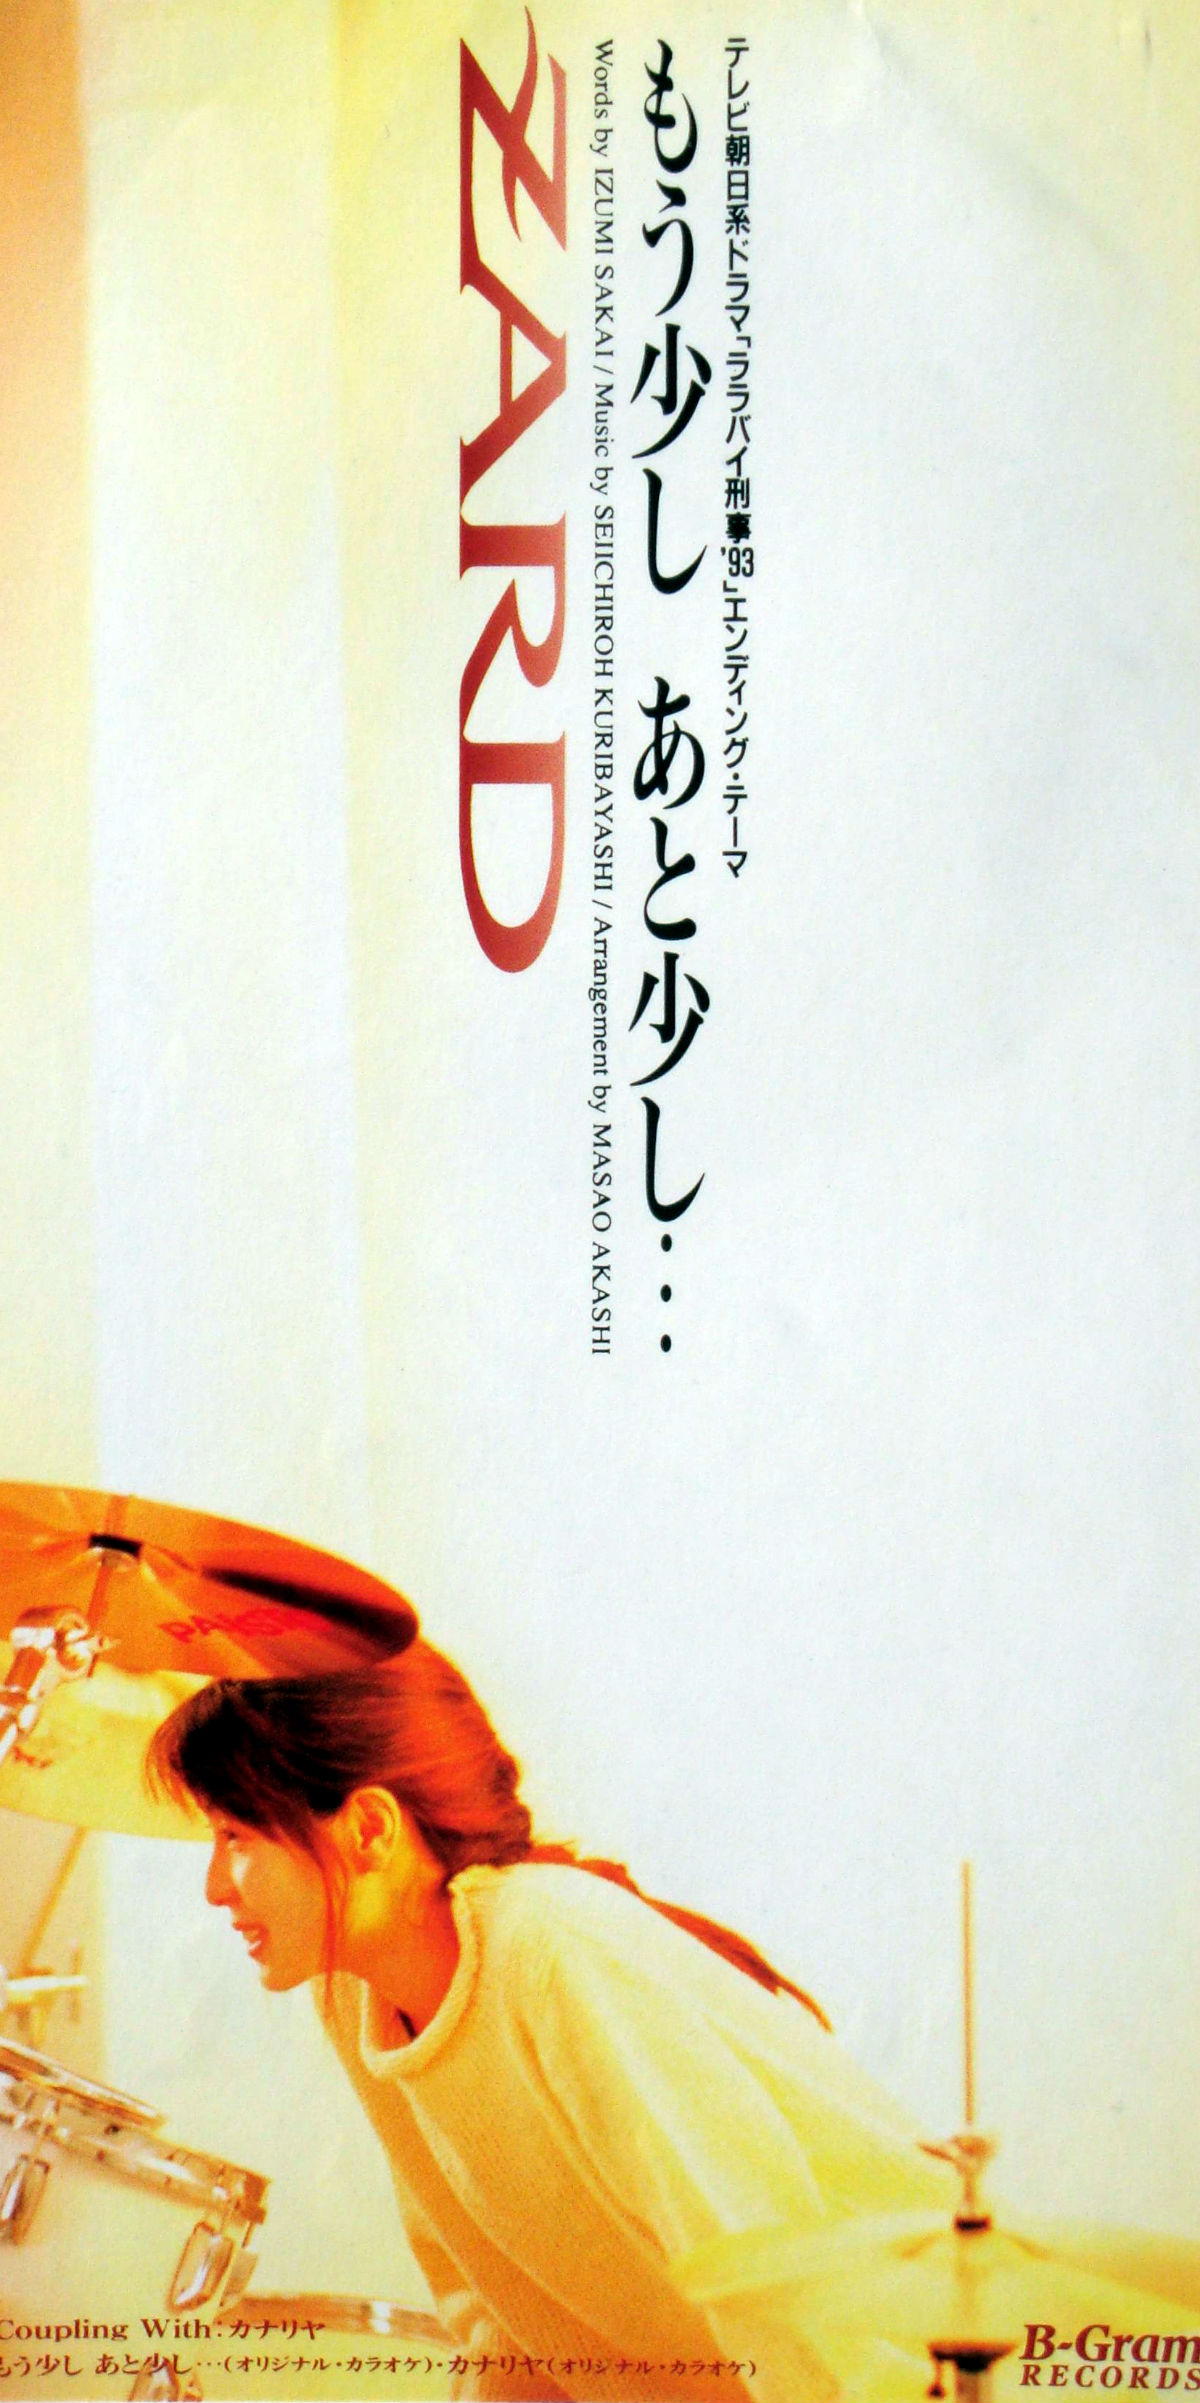
\includegraphics[width=0.3\textwidth]{S9.jpg}}

\large{

きまぐれな\ruby{九月}{くがつ}の\ruby{雨}{あめ}に

\ruby{白}{しろ}い\ruby{傘}{かさ}の\ruby{少女}{しょうじょ}がすれ\ruby{違}{ちが}う

\ruby{探}{さが}してた \ruby{二人}{ふたり}の\ruby{行方}{ゆくえ}

\ruby{今}{いま}はまだ \ruby{知}{し}りたくない

あなたの\ruby{揺}{ゆ}りかごの\ruby{中}{なか} そっと\ruby{眠}{ねむ}りたい

\ruby{心}{こころ}に\ruby{秘}{ひ}めた\ruby{涙}{なみだ}\ruby{忘}{わす}れ
\\

もう\ruby{少}{すこ}し あと\ruby{少}{すこ}し \ruby{愛}{あい}されたい

いけない\ruby{恋}{こい}と\ruby{知}{し}っても

もう\ruby{少}{しこ}し あなたのこと \ruby{困}{こま}らせたい

この\ruby{愛}{あい}\ruby{止}{と}められない
\\

\ruby{想}{おも}い\ruby{出}{で}の\ruby{神戸}{こうべ}の\ruby{街}{まち}で

あなたへの\ruby{手紙}{てがみ}したためています

\ruby{忘}{わす}れようと \ruby{何度}{なんど}もしたわ

その\ruby{方}{ほう}が\ruby{楽}{らく}になれる

\ruby{追伸}{ついしん}:あなたの\ruby{生}{う}まれた\ruby{家}{いえ}を\ruby{見}{み}てきました

なんだか \ruby{切}{せつ}なくて\ruby{懐}{なつか}しかった…
\\

もう\ruby{少}{すこ}し あと\ruby{少}{すこ}し そばにいたい

\ruby{叶}{かな}わぬ\ruby{夢}{ゆめ}と\ruby{知}{し}っても

そう\ruby{少}{すこ}し あの\ruby{女性}{ひと}より \ruby{出逢}{であ}う\ruby{時}{とき}が

\ruby{遅}{おそ}すぎただけなの
\\

もう\ruby{少}{すこ}し あと\ruby{少}{すこ}し \ruby{愛}{あい}されたい

いけない\ruby{恋}{こい}と\ruby{知}{し}っても

もう\ruby{少}{しこ}し あなたのこと \ruby{困}{こま}らせたい

この\ruby{愛}{あい}\ruby{止}{と}められない

}

\hypertarget{5_4}{}
\section{ 雨に濡れて}
\large{

\ruby{古}{ふる}い\ruby{ビル}{building}に\ruby{逃}{に}げこんだ MOON

\ruby{街}{まち}は\ruby{眠}{ねむ}ってる…

\ruby{30分}{ぷん}\ruby{早}{はや}く ついた\ruby{駅}{えき}の\ruby{ホーム}{home}

\ruby{感}{かん}じてた\ruby{別}{わか}れ…でも
\\

\ruby{乱用}{らんよう}しないで そのやさしさが

\ruby{誰}{だれ}かを\ruby{傷}{きず}つける

\ruby{今日}{きょう}で\ruby{二人}{ふたり}は \ruby{他人}{たにん}\ruby{同志}{どうし}だから

\ruby{別々}{べつべつ}に \ruby{帰}{かえ}ろう
\\

\ruby{雨}{あめ}に\ruby{濡}{ぬ}れて \ruby{想}{おも}い\ruby{出}{で}ごと \ruby{流}{なが}して

あなたのこと \ruby{忘}{わす}れられたら

\ruby{雨}{あめ}に\ruby{濡}{ぬ}れて \ruby{歩}{ある}き\ruby{続}{つづ}ける\ruby{歩道}{ほどう}に

\ruby{涙}{なみだ}の\ruby{色}{いろ}にじんで…
\\

いつか\ruby{車}{くるま}の\ruby{ボンネット}{bonnet}に

\ruby{指}{ゆび}で\ruby{書}{か}いた I LOVE YOU

\ruby{若}{わか}すぎた\ruby{日々}{ひび}の \ruby{思}{おも}い\ruby{出}{で}が\ruby{此処}{ここ}に

\ruby{月日}{とき}の\ruby{重}{おも}さ\ruby{知}{し}ったよ

もしもあの\ruby{日}{ひ}に\ruby{別}{べつ}の\ruby{道}{みち}を

\ruby{選}{えら}んでいたなら…

\ruby{少}{すこ}し \ruby{愛}{あい}し\ruby{方}{かた} \ruby{間違}{まちが}えただけで

すべては \ruby{エピローグ}{epilogue}
\\

\ruby{雨}{あめ}に\ruby{濡}{ぬ}れて この\ruby{孤独}{こどく}を\ruby{消}{き}したい

サヨナラだけ \ruby{胸}{むね}にひびく

\ruby{雨}{あめ}に\ruby{濡}{ぬ}れて \ruby{霞}{かす}む\ruby{二人}{ふたり}の

\ruby{記憶}{きおく}を \ruby{感}{かん}じていたい \ruby{今}{いま}だけは…
\\

\ruby{雨}{あめ}に\ruby{濡}{ぬ}れて \ruby{想}{おも}い\ruby{出}{で}ごと \ruby{流}{なが}して

あなたのこと \ruby{忘}{わす}れられたら

\ruby{雨}{あめ}に\ruby{濡}{ぬ}れて \ruby{歩}{ある}き\ruby{続}{つづ}ける\ruby{歩道}{ほどう}に

\ruby{涙}{なみだ}の\ruby{色}{いろ}にじんで…
\\

\ruby{雨}{あめ}に\ruby{濡}{ぬ}れて \ruby{霞}{かす}む\ruby{二人}{ふたり}の

\ruby{記憶}{きおく}を \ruby{感}{かん}じていたい \ruby{今}{いま}だけは…

}

\hypertarget{5_5}{}
\section{ この愛に泳ぎ疲れても}

\parpic[r]{
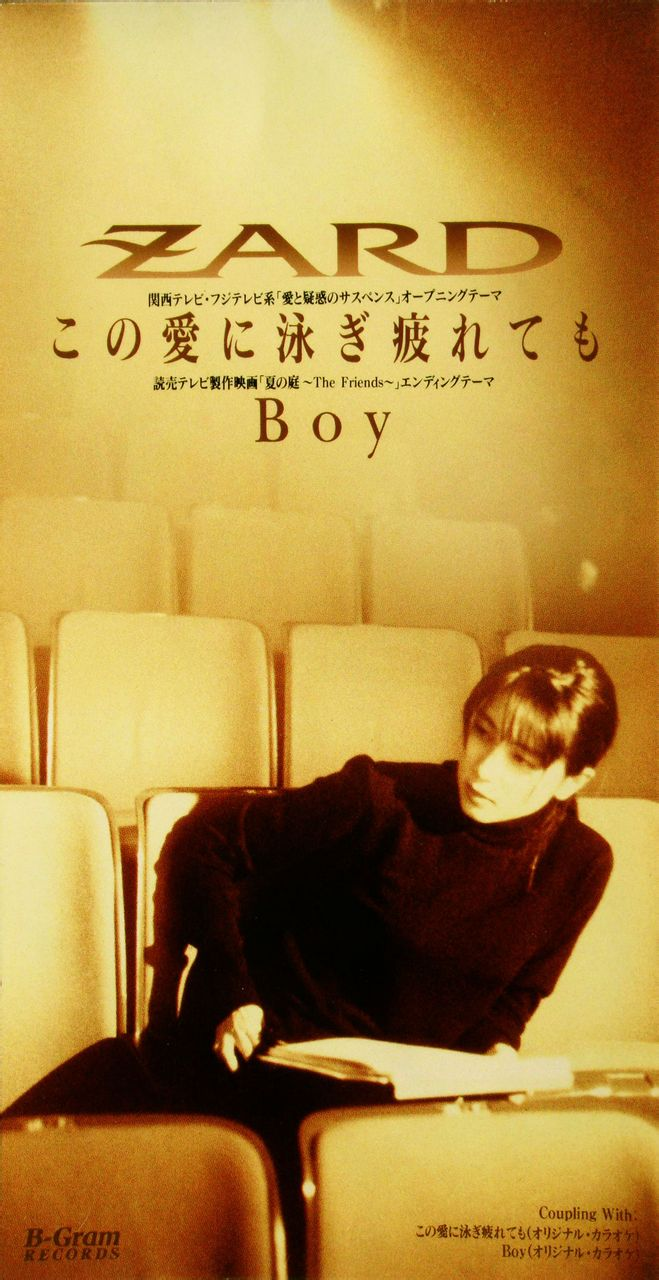
\includegraphics[width=0.3\textwidth]{S11.jpg}}

\large{

この\ruby{愛}{あい}に\ruby{泳}{およ}ぎ\ruby{疲}{つか}れても

もうひき\ruby{返}{かえ}さない

たどりつく\ruby{日}{ひ}まで
\\

すれ\ruby{違}{ちが}う\ruby{恋人達}{こいびとたち}

\ruby{バスケット}{Basket}\ruby{一杯}{いっぱい}の\ruby{夢}{ゆめ}を

\ruby{抱}{かか}えながら\ruby{歩}{ある}く

まるであの\ruby{頃}{ころ}のあなたと\ruby{私}{わたし}

\ruby{懐}{なつ}かしさに \ruby{振}{ふ}り\ruby{向}{む}いた
\\

この\ruby{愛}{あい}に\ruby{泳}{およ}ぎ\ruby{疲}{つか}れても

\ruby{流}{なが}されぬ\ruby{様}{よう}に \ruby{勇気}{ゆうき}を\ruby{与}{あた}えて

\ruby{出合}{であ}ってしまった \ruby{週末}{しゅうまつ}の\ruby{雨}{あめ}に

あなたとの\ruby{運命}{うんめい} \ruby{感}{かん}じた

\ruby{傷}{きづ}ついてもいい… \ruby{愛}{あい}したい
\\

いくつ\ruby{恋}{こい}を\ruby{重}{かさ}ねても

いつも\ruby{心}{こころ}\ruby{震}{ふる}えるの

\ruby{無口}{むくち}なあなただから

\ruby{不安}{ふあん}な\ruby{時}{とき}もある

だけど\ruby{少女}{しょうじょ}のように\ruby{泣}{な}けない
\\

このまま
\\

この\ruby{愛}{あい}に\ruby{泳}{およ}ぎ\ruby{疲}{つか}れても

もうひき\ruby{返}{かえ}せない

ふたつの\ruby{足跡}{あしあと}

\ruby{失}{な}くすものなんて \ruby{思}{おも}う\ruby{程}{ほど}ないから

そう \ruby{裸}{はだか}の\ruby{自分}{じぶん}になって

\ruby{愛}{あい}を\ruby{計}{はか}るより… \ruby{愛}{あい}したい
\\

この\ruby{愛}{あい}に\ruby{泳}{およ}ぎ\ruby{疲}{つか}れても

\ruby{流}{なが}されぬ\ruby{様}{よう}に \ruby{勇気}{ゆうき}を\ruby{与}{あた}えて

\ruby{出合}{であ}ってしまった \ruby{週末}{しゅうまつ}の\ruby{雨}{あめ}に

あなたとの\ruby{運命}{うんめい} \ruby{感}{かん}じた

\ruby{傷}{きづ}ついてもいい… \ruby{愛}{あい}したい

}

\hypertarget{5_6}{}
\section{ I still remember}
\large{

\ruby{波打}{なみう}ち\ruby{際}{ぎわ}を ひとりきり

すべる\ruby{太陽}{たいよう}に

\ruby{ホテル}{hotel}の\ruby{午後}{ごご}は ひとけもなくて

\ruby{時間}{とき}だけが \ruby{流}{なが}れてる

\ruby{無言}{むごん}で\ruby{切}{き}った\ruby{電話}{でんわ}に

\ruby{私}{わたし}だと\ruby{気付}{きづ}くわ

そう\ruby{願}{ねが}いをかけて

あなたの\ruby{連絡}{れんらく} どこかで\ruby{待}{ま}ってた
\\

I still remember

どうして\ruby{愛}{あい}は この\ruby{胸}{むね}ひき\ruby{裂}{さ}くの

\ruby{優}{やさ}しい\ruby{言葉}{ことば}で\ruby{別}{わか}れを\ruby{告}{つ}げた

あなたはずるい\ruby{人}{ひと}

ああ どんなにあなたを\ruby{呼}{よ}んでも

\ruby{風}{かぜ}に\ruby{消}{き}えてゆくのね

\ruby{二人}{ふたり}はもどれない\ruby{道}{みち}を ただ

\ruby{步}{ある}いてゆくだけなの
\\

\ruby{出合}{であ}って\ruby{二年}{にねん}の\ruby{月日}{つきひ}は \ruby{長}{なが}くて\ruby{短}{みじか}かった

\ruby{終}{お}わってしまえば\ruby{花火}{はなび}のようね

\ruby{夜空}{よぞら}に\ruby{夢見}{ゆめみ}て

\ruby{今頃}{いまごろ}あなたの\ruby{横}{よこ}には

\ruby{私}{わたし}よりやさしい\ruby{彼女}{かのじょ}がいると

\ruby{想像}{そうぞう}が\ruby{先走}{さきばし}る

\ruby{確}{たし}かめたいけど
\\

I still remember

あなたと\ruby{過}{す}ごした

\ruby{楽}{たの}しい\ruby{想}{おも}い\ruby{出}{で}ばかりが

\ruby{浮}{う}かんでは\ruby{心}{こころ}をかき\ruby{乱}{みだ}すの

\ruby{愛}{あい}はいじわる

ああ どんなにあなたを\ruby{呼}{よ}んでも

\ruby{思}{おも}いは\ruby{屆}{とど}かない

\ruby{二人}{ふたり}はもどること \ruby{知}{し}らずに

ここから\ruby{步}{ある}いて\ruby{行}{ゆ}くのね
\\

I still remember

どうして\ruby{愛}{あい}は この\ruby{胸}{むね}ひき\ruby{裂}{さ}くの

\ruby{優}{やさ}しい\ruby{言葉}{ことば}で\ruby{別}{わか}れを\ruby{告}{つ}げた

あなたはずるい\ruby{人}{ひと}
\\

I still remember

あなたを\ruby{呼}{よ}んでも

\ruby{風}{かぜ}に\ruby{消}{き}えてゆくのね

\ruby{二人}{ふたり}はもどれない\ruby{道}{みち}を ただ

\ruby{步}{ある}いてゆくだけなの

}

\hypertarget{5_7}{}
\section{ If you gimme smile}
\large{

If you gimme smile

\ruby{大地}{だいち}\ruby{蹴}{け}とばし \ruby{雲}{くも}の\ruby{流}{なが}れに

\ruby{忘}{わす}れよう \ruby{都会}{とかい}の\ruby{雜音}{ざつおん}…

ねえ \ruby{地平線}{ちへいせん}\ruby{広}{ひろ}がる
\\

\ruby{青}{あお}い Winding road

Oh \ruby{25}{にじゅうご}\ruby{マイル}{mile} \ruby{南}{みなみ}へ\ruby{行}{い}こう

\ruby{小}{ちい}さな\ruby{ボストンバック}{Bostonback}ひとつで

\ruby{熱}{あつ}い\ruby{風}{かぜ}に Singing out woo…
\\

If you gimme smile

なんて ちっぽけな\ruby{夢}{ゆめ}だたの

\ruby{恋}{こい}なんて\ruby{季節}{きせつ}の\ruby{ボーダーライン}{borderline}

Won't you gimme smile

\ruby{人生}{じんせい}の\ruby{地図}{ちず}に\ruby{コイン}{coin}\ruby{投}{な}げて

\ruby{賭}{か}けてみようよ \ruby{自分}{じぶん}に

So you can dream…
\\

Last night \ruby{テキーラ}{tequila}の

\ruby{苦}{にが}さに \ruby{孤独}{こどく}\ruby{愛}{あい}し

\ruby{現実}{げんじつ}に\ruby{目}{め}が\ruby{覚}{さ}めて \ruby{太陽}{たいよう}の\ruby{シャワー}{shower}

しがらみ\ruby{捨}{す}てて \ruby{明日}{あした}を\ruby{探}{さが}そう

\ruby{自由}{じゆう}に\ruby{生}{い}きてみたいね
\\

If you gimme smile

\ruby{大地}{だいち}\ruby{蹴}{け}とばし \ruby{雲}{くも}の\ruby{流}{なが}れに

\ruby{忘}{わす}れよう \ruby{都会}{とかい}の\ruby{雜音}{ざつおん}

Won't you gimme smile

\ruby{恋}{こい}は\ruby{ルーレット}{roulette} めぐりめぐる

\ruby{気}{き}のいい\ruby{家族}{かぞく}が\ruby{恋}{こい}しい

So you can dream…
\\

If you gimme smile I'm on your side

Tomorrow we'll be all right

We can take a chance so baby try now
\\

Wont you gimme smile

\ruby{人生}{じんせい}の\ruby{地図}{ちず}に\ruby{コイン}{coin}\ruby{投}{な}げて

\ruby{賭}{か}けてみようよ \ruby{自分}{じぶん}に

So we can dream

}

\hypertarget{5_8}{}
\section{ 来年の夏も}
\large{

\ruby{同}{おな}じ\ruby{血液型}{けつえきがた}\ruby{同士}{どうし}って

うまくいかないと いうけど

\ruby{私達}{わたしたち}\ruby{例外}{れいがい}ね \ruby{今}{いま}も

\ruby{2年前}{にねんまえ}の\ruby{気持}{きも}ちと \ruby{変}{か}わらない

\ruby{恋}{こい}の\ruby{予感}{よかん}は \ruby{土曜日}{どようび}の\ruby{映画館}{えいがかん}

\ruby{勇気}{ゆうき}を\ruby{出}{だ}してよかった…
\\

\ruby{来年}{らいねん}の\ruby{夏}{なつ}も となりにいるのが

どうか あなたでありますように
\\

\ruby{知}{し}り\ruby{合}{あ}う\ruby{前}{まえ}の\ruby{私}{わたし}は

“\ruby{強}{つよ}い\ruby{女}{おんな}”の\ruby{看板}{かんばん} \ruby{背負}{せお}ってた

あなたの\ruby{愛}{あい}の\ruby{レッスン}{lesson}で

\ruby{弱}{よわ}い\ruby{自分}{じぶん}も\ruby{好}{す}きになれたの

\ruby{ラベンダー}{lavender}の\ruby{匂}{にお}いに \ruby{心}{こころ}ときめく

\ruby{昨日}{きのう}よりもっと \ruby{愛}{いと}しい
\\

\ruby{来年}{らいねん}の\ruby{夏}{なつ}も となりにいるのが

どうか \ruby{私}{わたし}でありますように
\\

\ruby{時間}{じかん}\ruby{旅行}{りょこう}をしているみたいに

\ruby{景色}{けしき}だけが\ruby{変}{か}わってゆく
\\

\ruby{来年}{らいねん}の\ruby{夏}{なつ}も \ruby{二人}{ふたり}の\ruby{記念日}{きねんび}

\ruby{出会}{であ}った\ruby{場所}{ばしょ}でお\ruby{祝}{いわ}いしましょう

これからもずっと となりにいるのが

どうか あなたでありますように

}

\hypertarget{5_9}{}
\section{ あなたに帰りたい}
\large{

\ruby{泣}{な}いてばかりいた

あなたと\ruby{別}{わか}れてからずっと

もうすぐ\ruby{桜}{さくら}のさく\ruby{頃}{ころ}

この\ruby{頃}{ころ} \ruby{変}{か}わりました…
\\

\ruby{髪}{かみ}を\ruby{切}{き}って \ruby{明}{あか}るい\ruby{服}{ふく}を\ruby{着}{き}て

\ruby{目立}{めだ}たなかった

あの\ruby{日}{ひ}の\ruby{私}{わたし}に GOOD-BYE

\ruby{今度}{こんど}\ruby{会}{あ}っても そう\ruby{気付}{きづ}かないでしょう

そして もう\ruby{一度}{いちど}

あなたに\ruby{帰}{かえ}りたい
\\

\ruby{今}{いま}の\ruby{私}{わたし}なら\ruby{少}{すこ}しは

あなたに\ruby{追}{お}いつける?

せまい\ruby{街}{まち}だから

\ruby{時々}{ときどき}\ruby{見}{み}かけてしまうの
\\

\ruby{恋}{こい}をして \ruby{マリオネット}{marionette}のように

ただ\ruby{遠}{とお}くから あなたを\ruby{見守}{みまも}ってた

\ruby{今度}{こんど}\ruby{会}{あ}ったら \ruby{私}{わたし}に\ruby{気付}{きづ}いてね

そして もう\ruby{一度}{いちど}

\ruby{悲}{かな}しい\ruby{思}{おも}い\ruby{出}{で}に GOOD-BYE
\\

\ruby{髪}{かみ}を\ruby{切}{き}って \ruby{明}{あか}るい\ruby{服}{ふく}を\ruby{着}{き}て

\ruby{目立}{めだ}たなかった

あの\ruby{日}{ひ}の\ruby{私}{わたし}に GOOD-BYE

\ruby{今度}{こんど}\ruby{会}{あ}っても \ruby{私}{わたし}に\ruby{気付}{きづ}いてね

そして もう\ruby{一度}{いちど}

あなたに\ruby{帰}{かえ}りたい…

}
{ \ }

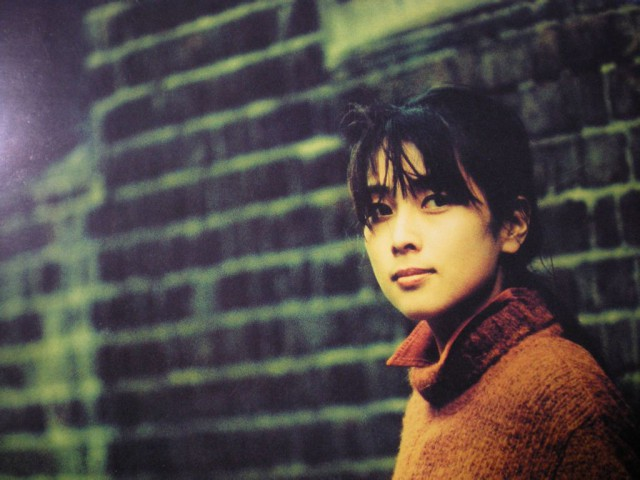
\includegraphics[width=0.7\textwidth]{P2.jpg}


\chapter{Album 6}
\thispagestyle{empty} %本页頁碼空白
\vspace{-16mm}
\LARGE {forever you}

\normalsize{JBCJ-1001 1995.3.10 \ release}
\\

\vspace{-5mm}

\parpic[l]{
\pichskip{6em}
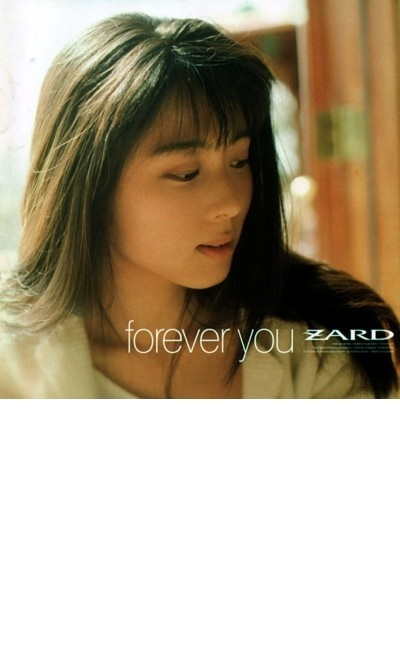
\includegraphics[width=0.4\textwidth]{6.jpg}}

\small{\hyperlink{6_0}{1.今すぐ会いに来て}}

\tiny{作詞:坂井泉水 \ 作曲:栗林誠一郎 \ 編曲:明石昌夫}

\small{\hyperlink{6_1}{2.ハイヒール脱ぎ捨てて}}

\tiny{作詞:坂井泉水 \ 作曲:栗林誠一郎 \ 編曲:明石昌夫}

\small{\hyperlink{6_2}{3.Forever you}}

\tiny{作詞:坂井泉水 \ 作曲:織田哲郎 \ 編曲:明石昌夫}

\small{\hyperlink{6_3}{4.もう逃げたりしないわ 想い出から}}

\tiny{作詞:坂井泉水 \ 作曲:栗林誠一郎 \ 編曲:明石昌夫}

\small{\hyperlink{6_4}{5.あなたを感じていたい}}

\tiny{作詞:坂井泉水 \ 作曲/編曲:織田哲郎}

\small{\hyperlink{6_5}{6.気楽に行こう}}

\tiny{作詞:坂井泉水 \ 作曲:栗林誠一郎 \ 編曲:池田大介}

\small{\hyperlink{6_6}{7.I'm in love}}

\tiny{作詞:坂井泉水 \ 作曲:織田哲郎 \ 編曲:池田大介}

\small{\hyperlink{6_7}{8.こんなにそばに居るのに}}

\tiny{作詞:坂井泉水 \ 作曲:栗林誠一郎 \ 編曲:明石昌夫}

\small{\hyperlink{6_8}{9.Just believe in love}}

\tiny{作詞:坂井泉水 \ 作曲:春畑道哉 \ 編曲:葉山たけし}

\small{\hyperlink{6_9}{10.瞳そらさないで}}

\tiny{作詞:坂井泉水 \ 作曲:織田哲郎 \ 編曲:明石昌夫}

\small{ \ }

\tiny{ \ }

\small{ \ }

\tiny{ \ }

\small{ \ }

\tiny{ \ }

\clearpage


\hypertarget{6_0}{}
\section{ 今すぐ会いに来て}
\large{

いつもあなたは\ruby{クール}{Cool}と\ruby{誤解}{ごかい}されてる

\ruby{本当}{ほんとう}は\ruby{誰}{だれ}より\ruby{傷}{きず}つきやすいのに

\ruby{人}{ひと}は\ruby{肩書}{みかけ}に\ruby{弱}{よわ}い \ruby{私}{わたし}だけは\ruby{味方}{みかた}よ
\\

\ruby{矛盾}{むじゅん}してるの \ruby{離}{はな}れている\ruby{時}{とき}は\ruby{心配}{しんぱい}なのに

\ruby{会}{あ}うとすぐに \ruby{自我}{じが}と\ruby{独占}{どくせん}\ruby{欲}{よく}と\ruby{強}{つよ}がりが\ruby{出}{で}ちゃうの
\\

だって お\ruby{互}{たが}い\ruby{少}{すこ}し\ruby{見}{み}えない\ruby{部分}{ぶぶん}があった\ruby{方}{ほう}がいい

だけど \ruby{ジェラシー}{Jealousy}の\ruby{変化球}{へんかきゅう}

\ruby{嘘}{うそ}ならやさしく\ruby{投}{な}げてね
\\

\ruby{今}{いま}すぐ\ruby{会}{あ}いに\ruby{来}{き}て \ruby{次}{つぎ}の\ruby{約束}{やくそく}まで

\ruby{待}{ま}てそうにないくらい \ruby{素敵}{すてき}な\ruby{恋人}{こいびと}
\\

“\ruby{センチメンタル}{Sentimental}”“\ruby{ロマンティック}{Romantic}”

どれもあなたに\ruby{似合}{にあ}わない

だけど さり\ruby{気}{き}なく\ruby{私}{わたし}の\ruby{前}{まえ}を\ruby{歩}{ある}いてくれる\ruby{人}{ひと}
\\

\ruby{今}{いま}すぐ\ruby{会}{あ}いに\ruby{来}{き}て その\ruby{笑顔}{えがお}が\ruby{好}{す}きよ

せつない\ruby{夜}{よる}がいっぱい \ruby{土曜日}{どようび}の\ruby{恋人}{こいびと}
\\

La La La …

La La La …
\\

\ruby{明日}{あした}の\ruby{地図}{ちず}を\ruby{探}{さが}そう \ruby{ベージュ}{Beige}の\ruby{シャツ}{Shirt}に\ruby{手}{て}を\ruby{振}{ふ}った

}

\hypertarget{6_1}{}
\section{ ハイヒール脱ぎ捨てて}
\large{

\ruby{四月前}{しがつまえ}の\ruby{電車}{でんしゃ}は

\ruby{学生服}{がくせいふく}も まばらで

\ruby{窓}{まど}の\ruby{外}{そと}の\ruby{生活}{せいかつ}の\ruby{音}{おと}だけ

いつも いつも \ruby{変}{か}わらない

\ruby{今}{いま}なら \ruby{仕事}{しごと}と\ruby{恋}{こい}に\ruby{揺}{ゆ}れたりしないわ

あの\ruby{日}{ひ} あなたという\ruby{ホームグラウンド}{Home Ground}から

\ruby{旅立}{たびだ}った\ruby{私}{わたし}を \ruby{許}{ゆる}して
\\

\ruby{ハイヒール}{High-heel}\ruby{脱}{ぬ}ぎ\ruby{捨}{す}てて

\ruby{青}{あお}い\ruby{海}{うみ}が\ruby{見}{み}たいわ

\ruby{二人}{ふたり}でよく\ruby{行}{い}ったから

\ruby{懐}{なつ}かしい\ruby{サイドシート}{Side Sheet}

\ruby{私}{わたし}の\ruby{居場所}{いばしょ}はある?

あぁ \ruby{笑顔}{えがお}も\ruby{痩}{や}せてゆく
\\

\ruby{昔}{むかし}の\ruby{友達}{ともだち}は みんな\ruby{変}{か}わってしまったし

\ruby{皮肉}{ひにく}すぎる \ruby{今}{いま}の\ruby{私}{わたし}には

また あなたしかいないなんて
\\

\ruby{思}{おも}い\ruby{出}{で}を \ruby{脱}{ぬ}ぎ\ruby{捨}{す}てて

\ruby{青}{あお}い\ruby{海}{うみ}が\ruby{見}{み}たいわ

\ruby{話}{はな}したいことがいっぱい

\ruby{白}{しろ}い\ruby{Tシャツ}{T-Shirt} \ruby{ブルージーンズ}{Blue Jeans}

そして\ruby{素顔}{すがお}の\ruby{私}{わたし}を

おもいきり \ruby{抱}{だ}きしめて
\\

\ruby{後悔}{こうかい}を \ruby{脱}{ぬ}ぎ\ruby{捨}{す}てて

\ruby{青}{あお}い\ruby{海}{うみ}が\ruby{見}{み}たいわ

\ruby{話}{はな}したいことがいっぱい

\ruby{白}{しろ}い\ruby{Tシャツ}{T-Shirt} \ruby{ブルージーンズ}{Blue Jeans}

そして\ruby{素顔}{すがお}の\ruby{私}{わたし}を

おもいきり \ruby{抱}{だ}きしめて
\\

\ruby{ハイヒール}{High-heel}\ruby{脱}{ぬ}ぎ\ruby{捨}{す}てて

あの\ruby{夏}{なつ}の\ruby{日}{ひ}のlast dance

もう\ruby{一度}{いちど} \ruby{踊}{おど}るたいの

}

\hypertarget{6_2}{}
\section{ forever you}
\large{

\ruby{若}{わか}い\ruby{頃}{ころ}は\ruby{人}{ひと}\ruby{一倍}{いちばい}\ruby{好奇心}{こうきしん}が\ruby{強}{つよ}くて

いろんな\ruby{周囲}{まわり}の\ruby{人}{ひと}や\ruby{家族}{かぞく}に\ruby{迷惑}{めいわく}ばかりかけてた
\\

\ruby{手}{て}さぐりで\ruby{夢}{ゆめ}を\ruby{探}{さが}していた あの\ruby{日}{ひ}

\ruby{自分}{じぶん}が\ruby{將来}{あした}どんな\ruby{風}{ふう}になるのかわからなくて ただ

\ruby{前}{まえ}に\ruby{進}{すす}むことばかり\ruby{考}{かんが}えていた Dear old days
\\

もう\ruby{泣}{な}かないで やっと \ruby{夢}{ゆめ}が\ruby{叶}{かな}った

ずっと… forever you

そう あせらずに そう \ruby{急}{いそ}がずに \ruby{大人}{おとな}になりたい
\\

たくさん\ruby{失敗}{しっばい}もしたけど いつもそんな\ruby{時}{とき}

\ruby{優}{やさ}しく\ruby{親切}{しんせつ}だった\ruby{人達}{ひとたち}の\ruby{笑顔}{えがお}が\ruby{浮}{う}かんだ \ruby{涙}{なみだ}も\ruby{忘}{わす}れた

\ruby{自分}{じぶん}で\ruby{選}{えら}んだ\ruby{道}{みち}だから
\\

もう\ruby{迷}{まよ}わない \ruby{今}{いま}が\ruby{幸}{しあわ}せだから

ずっと… forever you

そう あせらずに そう \ruby{急}{いそ}がずに \ruby{愛}{あい}したいの
\\

それは\ruby{暖}{あたた}かいあなたに\ruby{出逢}{であ}うまでの\ruby{試練}{しれん}

\ruby{過去}{むかし}に\ruby{後悔}{こうかい}なんてしてない

またとない \ruby{二度}{にど}と\ruby{来}{こ}ない \ruby{私}{わたし}の\ruby{青春}{せいしゅん}だから
\\

So stay with me my love forever

}

\hypertarget{6_3}{}
\section{ もう逃げたりしないわ想い出から}
\large{

またここに\ruby{来}{く}るとは\ruby{思}{おも}わなかった

\ruby{苦}{にが}い\ruby{恋}{こい}が\ruby{詰}{つ}まった この\ruby{浜辺}{はまべ}に

はしゃぐ\ruby{彼}{なみ}には\ruby{言}{い}い\ruby{出}{だ}せなくて…

そんな\ruby{時}{とき} \ruby{言葉}{ことば}は\ruby{空回}{からまわ}りする

\ruby{沈}{しず}む\ruby{夕陽}{ゆうひ}のせいね \ruby{一瞬}{いっしゅん}

\ruby{彼}{かれ}とあなたがダブった
\\

もう\ruby{逃}{に}げたりしないわ \ruby{想}{おも}い\ruby{出}{で}から

\ruby{傷}{きず}つくこと\ruby{怖}{おそ}れない

\ruby{胸}{むね}の\ruby{中}{なか}\ruby{何}{なに}かが\ruby{弾}{はじ}けて\ruby{消}{き}えた
\\

やぶり\ruby{捨}{す}てた\ruby{壁}{かべ}の\ruby{5月}{ごがつ}の\ruby{カレンダー}{Calendar}

\ruby{時間}{とき}は\ruby{人}{ひと}の\ruby{気持}{きも}ちより\ruby{速}{はや}く\ruby{過}{す}ぎる

\ruby{悲}{かな}しかったのは\ruby{別}{わか}れの\ruby{言葉}{ことば}じゃない

\ruby{本当}{ほんとう}の\ruby{私}{わたし}を\ruby{知}{し}らなかった\ruby{事}{こと}

\ruby{今}{いま}\ruby{何処}{どこ}で\ruby{暮}{く}らしてますか

\ruby{東京}{まち}を\ruby{出}{で}たと\ruby{聞}{き}いた
\\

もう\ruby{逃}{に}げたりしないわ \ruby{想}{おも}い\ruby{出}{で}から

「あなたもきっと \ruby{悩}{なや}んだでしょう」

そんな\ruby{事}{こと}も\ruby{不思議}{ふしぎ}と\ruby{言}{い}える

もう\ruby{逃}{に}げたりしないわ \ruby{想}{おも}い\ruby{出}{で}から

あなたの\ruby{事}{こと} \ruby{忘}{わす}れない

だけどもうあなたの\ruby{事}{こと}で\ruby{泣}{な}かない

}

\hypertarget{6_4}{}
\section{ あなたを感じていたい}

\large{

ねぇ そんなにしゃべらなくても

\ruby{私}{わたし}\ruby{笑}{わら}っていられるから

もう\ruby{逢}{あ}えない\ruby{気}{き}がして…

\ruby{誰}{だれ}も\ruby{居}{い}ない \ruby{駅}{えき}の\ruby{ホーム}{Home}

それぞれの\ruby{冬}{ふゆ}\ruby{選}{えら}び \ruby{想}{おも}い\ruby{出}{で}に\ruby{手}{て}を\ruby{振}{ふ}った
\\

あなたを\ruby{感}{かん}じていたい

たとえ\ruby{遠}{とお}く \ruby{離}{はな}れていても

ときめく\ruby{心}{こころ} \ruby{止}{と}めないで

みんな\ruby{見}{み}えない\ruby{明日}{あした}を\ruby{探}{さが}している

\ruby{約束}{やくそく}なんて\ruby{何}{なに}もないけど

\ruby{変}{か}わらない\ruby{二人}{ふたり}でいようね
\\

ふるえる\ruby{口唇}{くちびる} ふさいで

\ruby{別}{わか}れ\ruby{際}{ぎわ} \ruby{言}{い}いかけた\ruby{言葉}{ことば}に

もう\ruby{逢}{あ}えない\ruby{気}{き}がした…

\ruby{独}{ひと}り\ruby{歩}{ある}く\ruby{街中}{まちじゅう}が にじんだ\ruby{キャンドル}{Candle}でいっぱい

\ruby{切}{せつ}なくて
\\

\parpic[r]{

\includegraphics[width=0.3\textwidth]{S13.jpg}}

あなたを\ruby{感}{かん}じていたい

\ruby{白}{しろ}い\ruby{吐息}{といき}の \ruby{季節}{きせつ}の\ruby{中}{なか}で

\ruby{今}{いま}すぐ\ruby{飛}{と}んでゆきたいけど

すべてを\ruby{捨}{す}てて\ruby{行}{ゆ}けない\ruby{私}{わたし}がいる

\ruby{口}{くち}に\ruby{出}{だ}さないやさしさが\ruby{痛}{いた}い

\ruby{窓}{まど}の\ruby{外}{そと}も\ruby{雪}{ゆき}に\ruby{変}{か}わった
\\

あなたを\ruby{感}{かん}じていたい

\ruby{銀色}{ぎんいろ}の\ruby{季節}{きせつ}の\ruby{中}{なか}で

\ruby{輝}{かがや}き\ruby{続}{つづ}けて\ruby{欲}{ほ}しい

だけど\ruby{都会}{とかい}の\ruby{スピード}{Speed}に\ruby{流}{なが}されないで

「\ruby{待}{ま}っているから」と どうしてあの\ruby{時}{とき}

\ruby{素直}{すなお}に\ruby{言}{い}えなかったのだろう…

}

\hypertarget{6_5}{}
\section{ 気楽に行こう}
\large{

\ruby{氣}{き}がつけば\ruby{私}{わたし} さっきから

\ruby{鳴}{な}らない\ruby{電話}{でんわ}ニラんでる

\ruby{少}{すこ}し\ruby{手}{て}\ruby{加減}{かげん}してもいいのに…

\ruby{長}{なが}い\ruby{付}{つ}き\ruby{合}{あ}いって

\ruby{素直}{すなお}じゃいられなくなるわ

\ruby{小}{ちい}さな\ruby{空}{そら}にため\ruby{息}{いき}ついた
\\

\ruby{氣樂}{きらく}に\ruby{行}{い}こう \ruby{今}{いま}は

\ruby{追}{お}いかけたい\ruby{氣持}{きも}ちにブレーキかけて

\ruby{忙}{いそが}しさに\ruby{寄}{よ}りかかりたい…

\ruby{風}{かぜ}が\ruby{止}{と}まった

\ruby{明日}{あした}はきっと\ruby{笑顏}{えがお}が\ruby{似合}{にあ}う
\\

コンクリートに\ruby{膝}{ひざ}を\ruby{抱}{だ}えて\ruby{座}{すわ}ったら

\ruby{世}{よ}の\ruby{中}{なか}が\ruby{見}{み}えた

\ruby{人}{ひと}ゴミの\ruby{視線}{しせん}が\ruby{私}{わたし}の\ruby{肩}{かた}を\ruby{抱}{だ}くけど

ああ こうしていたい\ruby{氣分}{きぶん}なの

やっぱり あなたに\ruby{會}{あ}いたい
\\

\ruby{氣樂}{きらく}に\ruby{行}{い}こう \ruby{今}{いま}は

\ruby{目}{め}の\ruby{前}{まえ}にあるそれぞれの\ruby{夢}{ゆめ}を

ひとつずつ\ruby{積}{つ}み\ruby{上}{あ}げていこう

\ruby{變}{か}わってしまったのは

あなたじゃなく \ruby{私}{わたし}なのかもしれない
\\

\ruby{氣樂}{きらく}に\ruby{行}{い}こう \ruby{今}{いま}は

ミラーに\ruby{映}{うつ}る\ruby{小}{ちい}さな\ruby{幸}{しあわ}せを

ひとつずつ\ruby{積}{つ}み\ruby{上}{あ}げていこう

\ruby{風}{かぜ}が\ruby{止}{と}まった

\ruby{二人}{ふたり}に\ruby{夏}{なつ}の\ruby{想}{おも}い\ruby{出}{で}\ruby{下}{くだ}さい

}

\hypertarget{6_6}{}
\section{ I'm in love}
\large{

\ruby{今日}{きょう}も\ruby{心}{こころ}\ruby{震}{ふる}わす\ruby{ニュース}{News}の\ruby{バレード}{Volleyball}

Oh! I feel so blue

\ruby{偽}{いつわ}りを\ruby{知}{し}らない\ruby{瞳}{め}が\ruby{ブラウン}{Brown}\ruby{管}{かん}からこっちを\ruby{見}{み}つめる

なんて\ruby{無力}{むりょく}なの \ruby{彼}{かれ}ら\ruby{救}{すく}えない

\ruby{私}{わたし}の\ruby{失望}{なやみ}は\ruby{小}{ちい}さすぎるわ
\\

I'm in love \ruby{時代}{じだい}はいつも \ruby{変}{か}わってゆくけど

\ruby{ヒーロー}{Hero}がいるわ

I'm in love \ruby{信}{しん}じる\ruby{者}{もの}は\ruby{救}{すく}われるのよ

\ruby{辛}{つら}くても いつか We got power of love
\\

お\ruby{隣}{とな}りの\ruby{顔}{かお}も\ruby{知}{し}らない

\ruby{冷凍食品}{レトルト}にも\ruby{飽}{あ}き\ruby{飽}{あ}きしてる

\ruby{常識}{じょうしき}は\ruby{打}{う}ちのめされた

\ruby{シングル}{Single}\ruby{ライフ}{Life}を\ruby{楽}{たの}しむ\ruby{彼女}{かのじょ}

No No!\ruby{何}{なに}か\ruby{忘}{わす}れてる \ruby{人間}{ひと}を\ruby{愛}{あい}するってこと

\ruby{環境}{かんきょう}\ruby{破壊}{はかい}よあなた\ruby{自身}{じしん}の
\\

I'm in love \ruby{時代}{じだい}はいつも \ruby{変}{か}わってゆくけど

\ruby{ヒーロー}{Hero}が\ruby{欲}{ほ}しい

I'm in love \ruby{闘}{たたか}うことに\ruby{疲}{つか}れても

そんな\ruby{時}{とき}こそ\ruby{淑女}{しゅくじょ}よ We got power of love
\\

I'm in love \ruby{時代}{じだい}はいつも \ruby{変}{か}わってゆくけど

\ruby{ヒーロー}{Hero}はいるわ

I'm in love \ruby{夜明}{よあ}けはいつかやって\ruby{来}{く}るのよ

\ruby{諦}{あきら}めないで We got power of love

}

\hypertarget{6_7}{}
\section{ こんなにそばに居るのに}

\large{

こんなにそばに\ruby{居}{い}るのに

\ruby{黙}{だま}らないで Lovin' you
\\

Summer night \ruby{何台}{なんだい}も\ruby{車}{くるま}\ruby{見送}{みおく}って

\ruby{途切}{とぎ}れた\ruby{隙}{すき}に Good night kiss

\ruby{偶然}{ぐうぜん}がまるで \ruby{運命}{うんめい}に\ruby{思}{おも}えたあの\ruby{頃}{ころ}

\ruby{グラス}{Glass}の\ruby{氷}{こおり}が カラカラ \ruby{揺}{ゆ}れてる

いつもの\ruby{レストラン}{Restaurant}で

\ruby{昔}{むかし}を\ruby{懐}{なつ}かしむのは きっと\ruby{二人}{ふたり}

\ruby{話題}{わだい}が\ruby{見}{み}つからないせい!?

あの\ruby{時}{とき} \ruby{時間}{じかん}が\ruby{止}{と}まったままなら…

\ruby{遠回}{とおまわ}りはしなかった
\\

\parpic[r]{
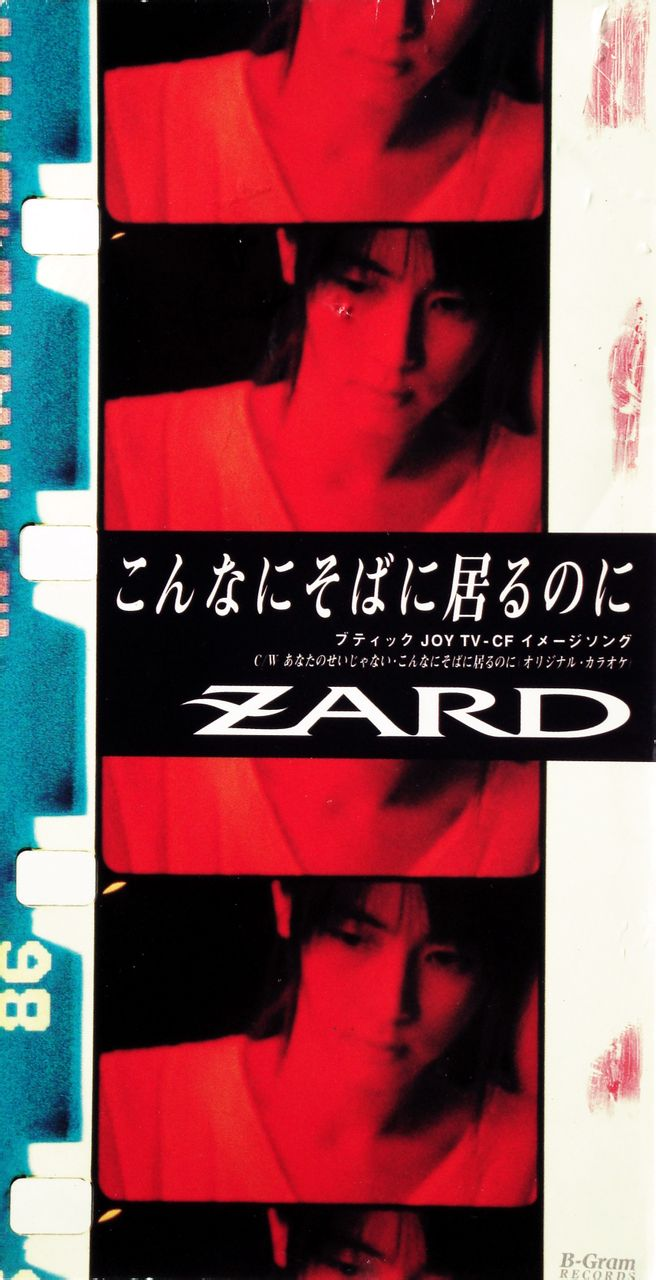
\includegraphics[width=0.3\textwidth]{S12.jpg}}

こんなにそばに\ruby{居}{い}るのに

\ruby{黙}{だま}らないで Lovin' you

\ruby{出会}{であ}った\ruby{頃}{ころ}のように \ruby{熱}{あつ}く\ruby{激}{はげ}しく

あなたの\ruby{汗}{あせ} \ruby{感}{かん}じてる

\ruby{真夏}{まなつ}のように Hold me tight

この\ruby{手}{て}を \ruby{放}{はな}さないで

この\ruby{愛}{あい} つかまえていて
\\

Summer love 

めざす\ruby{夢}{ゆめ}は\ruby{違}{ちが}ってたけど

\ruby{好}{す}きになれば 

\ruby{未来}{みらい}も\ruby{変}{か}わる

どんな\ruby{悲}{かな}しいウワサも 

\ruby{吹}{ふ}き\ruby{飛}{と}ぶような

\ruby{一途}{いちず}な\ruby{瞳}{ひとみ}を\ruby{信}{しん}じてた

\ruby{今}{いま}は まるで\ruby{迷}{まよ}い\ruby{道}{みち}の\ruby{中}{なか}

\ruby{二人}{ふたり}は\ruby{出口}{でぐち} \ruby{探}{さが}してる
\\

こんなにそばに\ruby{居}{い}るのに

\ruby{眠}{ねむ}らないで Lovin' you

\ruby{友達}{ともだち}より\ruby{遠}{とお}く\ruby{感}{かん}じるのよ

\ruby{離}{はな}れていく\ruby{心}{こころ}に \ruby{アクセル}{Accelerator}\ruby{強}{つよ}く Ride away

\ruby{震}{ふる}えるほど \ruby{見}{み}つめて

もう\ruby{一度}{いちど} \ruby{始}{はじ}めてみたい…
\\

こんなにそばに\ruby{居}{い}るのに

\ruby{黙}{だま}らないで Lovin' you

\ruby{出会}{であ}った\ruby{頃}{ころ}のように \ruby{熱}{あつ}く\ruby{激}{はげ}しく

あなたの\ruby{汗}{あせ} \ruby{感}{かん}じてる

\ruby{真夏}{まなつ}のように Hold me tight

この\ruby{手}{て}を \ruby{放}{はな}さないで

この\ruby{愛}{あい} つかまえていて

}

\hypertarget{6_8}{}
\section{ Just believe in love}
\large{

すりきれる\ruby{程}{ほど} \ruby{聴}{き}いた\ruby{アルバム}{Album}が

あの\ruby{頃}{ころ}たった\ruby{一人}{ひとり}の\ruby{友達}{ともだち}だった

\ruby{出逢}{であ}いと\ruby{別離}{わかれ}を\ruby{繰}{く}り\ruby{返}{かえ}し

\ruby{人}{ひと}は\ruby{大人}{おとな}になる

たどりついた \ruby{今}{いま}あなたに
\\

Just believe in love

あんなに\ruby{熱}{あつ}く\ruby{焦}{こ}がした\ruby{想}{おも}いが\ruby{揺}{ゆ}れている

\ruby{感}{かん}じてる あなたの\ruby{愛}{あい}を\ruby{身体中}{からだじゅう}

このまま\ruby{溶}{と}けてゆく \ruby{遊}{あそ}び\ruby{疲}{つか}れて\ruby{眠}{ねむ}る \ruby{子供}{こども}のように
\\

\ruby{降}{ふ}りしきる\ruby{雨}{あめ}が\ruby{虹}{にじ}に\ruby{変}{か}わる

\ruby{歳}{とし}の\ruby{差}{さ}の\ruby{迷}{まよ}いを\ruby{捨}{す}てて\ruby{飛}{と}び\ruby{込}{こ}んだ

\ruby{今}{いま} この\ruby{瞬間}{しゅんかん}に\ruby{夢}{ゆめ}が\ruby{覚}{さ}めてしまわぬように \ruby{強}{つよ}く

\ruby{抱}{だ}きしめて \ruby{私}{わたし}を
\\

Just believe in love

\ruby{形}{かたち}のない\ruby{愛}{あい}に\ruby{理由}{わけ}もなく \ruby{泣}{な}きたくなるけれど

\ruby{誰}{だれ}よりも あなたの\ruby{温}{ぬく}もり \ruby{信}{しん}じてる

\ruby{何}{なに}かに \ruby{傷}{きず}ついては…

そんなとこ\ruby{二人}{ふたり}は よく\ruby{似}{に}ているね
\\

Just believe in love

あんなに\ruby{熱}{あつ}く\ruby{焦}{こ}がした\ruby{想}{おも}いが\ruby{揺}{ゆ}れている

\ruby{微笑}{ほほえ}みも \ruby{忘}{わす}れたくなるこの\ruby{都会}{まち}で

つまずくことさえも \ruby{明日}{あす}への\ruby{希望}{きぼう}へと\ruby{変}{か}えてゆこう

\ruby{明日}{あす}への\ruby{希望}{きぼう}へと\ruby{変}{か}えてゆこう

}
{ \ }


\includegraphics[width=0.5\textwidth]{S14.jpg}

\hypertarget{6_9}{}
\section{ 瞳そらさないで}
\large{

いつも この\ruby{時間}{じかん}は\ruby{家}{うち}に\ruby{居}{い}たのに…

\ruby{最近}{さいきん}\ruby{君}{きみ}は \ruby{留守}{るす}がちだね

やっと\ruby{出}{で}た\ruby{電話}{でんわ}の\ruby{声}{こえ}も

\ruby{以前}{いま}までと\ruby{違}{ちが}う \ruby{感}{かん}じが\ruby{変}{か}わったよ

まだ \ruby{君}{きみ}の\ruby{中}{なか}に \ruby{僕}{ぼく}がどれくらい\ruby{居}{い}るのか

\ruby{確}{たし}かめてみたいんだ look in your eyes
\\

\ruby{瞳}{ひとみ}そらさないで \ruby{青}{あお}い\ruby{夏}{なつ}のトキメキの\ruby{中}{なか}で

summer breeze \ruby{心}{こころ}くすぐるよ

ひとり\ruby{占}{じ}めしたて \ruby{抱}{だ}き\ruby{寄}{よ}せた あつい\ruby{午後}{ごご}
\\

「\ruby{今}{いま}のままでは\ruby{視野}{しや}が\ruby{狭}{せま}くなるし…

\ruby{何}{なに}かが\ruby{終}{お}わってしまいそう」と\ruby{彼女}{かのじょ}が\ruby{云}{い}った

その\ruby{方}{ほう}が\ruby{君}{きみ}にとって\ruby{夢}{ゆめ}があるのなら

\ruby{僕}{ぼく}はそうしよう

“\ruby{約束}{やくそく}だから\ruby{海}{うみ}に\ruby{来}{き}た”って\ruby{感}{かん}じが

\ruby{一緒}{いっしょ}に\ruby{居}{い}るのに\ruby{淋}{さび}しいよ
\\

もう\ruby{一度}{いちど}…
\\

\ruby{話}{はな}しそらさないで \ruby{青}{あお}い\ruby{夏}{なつ}のトキメキの\ruby{中}{なか}で

summer days \ruby{想}{おも}い\ruby{出}{で}にしないで

あの\ruby{頃}{ころ}の \ruby{君}{きみ}が\ruby{今}{いま}も \ruby{胸}{むね}の\ruby{中}{なか}で\ruby{微笑}{わら}ってる

あの\ruby{頃}{ころ}の \ruby{君}{きみ}が\ruby{今}{いま}も \ruby{胸}{むね}の\ruby{中}{なか}で\ruby{微笑}{わら}ってる

}


\chapter{Album 7}
\thispagestyle{empty} %本页頁碼空白
\vspace{-16mm}
\LARGE {TODAY IS ANOTHER DAY}

\normalsize{JBCJ-1009 1996.7.8 \ release}
\\

\vspace{-5mm}

\parpic[l]{
\pichskip{6em}
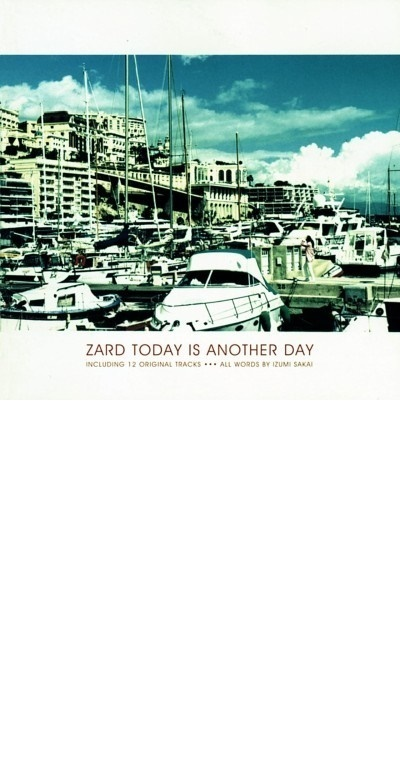
\includegraphics[width=0.4\textwidth]{7.jpg}}

\small{\hyperlink{7_0}{1.マイ フレンド}}

\tiny{作詞:坂井泉水 \ 作曲:織田哲郎 \ 編曲:葉山たけし}

\small{\hyperlink{7_1}{2.君がいたから}}

\tiny{作詞:坂井泉水 \ 作曲:織田哲郎 \ 編曲:葉山たけし}

\small{\hyperlink{7_2}{3.サヨナラは今もこの胸に居ます}}

\tiny{作詞:坂井泉水 作曲:栗林誠一郎 編曲:葉山たけし}

\small{\hyperlink{7_3}{4.Love ~眠れずに君の橫顏ずっと見ていた~}}

\tiny{作詞:坂井泉水 \ 作曲:栗林誠一郎 \ 編曲:明石昌夫}

\small{\hyperlink{7_4}{5.DAN DAN 心魅かれてく}}

\tiny{作詞:坂井泉水 \ 作曲:織田哲郎 \ 編曲:池田大介}

\small{\hyperlink{7_5}{6.眠り}}

\tiny{作詞/作曲:坂井泉水 編曲:池田大介}

\small{\hyperlink{7_6}{7.心を開いて}}

\tiny{作詞:坂井泉水 \ 作曲:織田哲郎 \ 編曲:池田大介}

\small{\hyperlink{7_7}{8.突然}}

\tiny{作詞:坂井泉水 \ 作曲:織田哲郎 \ 編曲:葉山たけし}

\small{\hyperlink{7_8}{9.今日も}}

\tiny{作詞:坂井泉水 \ 作曲:織田哲郎 \ 編曲:葉山たけし}

\small{\hyperlink{7_9}{10.TODAY IS ANOTER DAY}}

\tiny{作詞:坂井泉水 \ 作曲:織田哲郎 \ 編曲:池田大介}

\small{\hyperlink{7_10}{11.愛が見えない}}

\tiny{作詞:坂井泉水 \ 作曲:小澤正澄 \ 編曲:葉山たけし}

\small{\hyperlink{7_11}{12.見つめていたいね}}

\tiny{作詞:坂井泉水 \ 作曲:栗林誠一郎 \ 編曲:明石昌夫}

\small{ \ }

\tiny{ \ }


\clearpage


\hypertarget{7_0}{}
\section{ My Friend}

\parpic[r]{
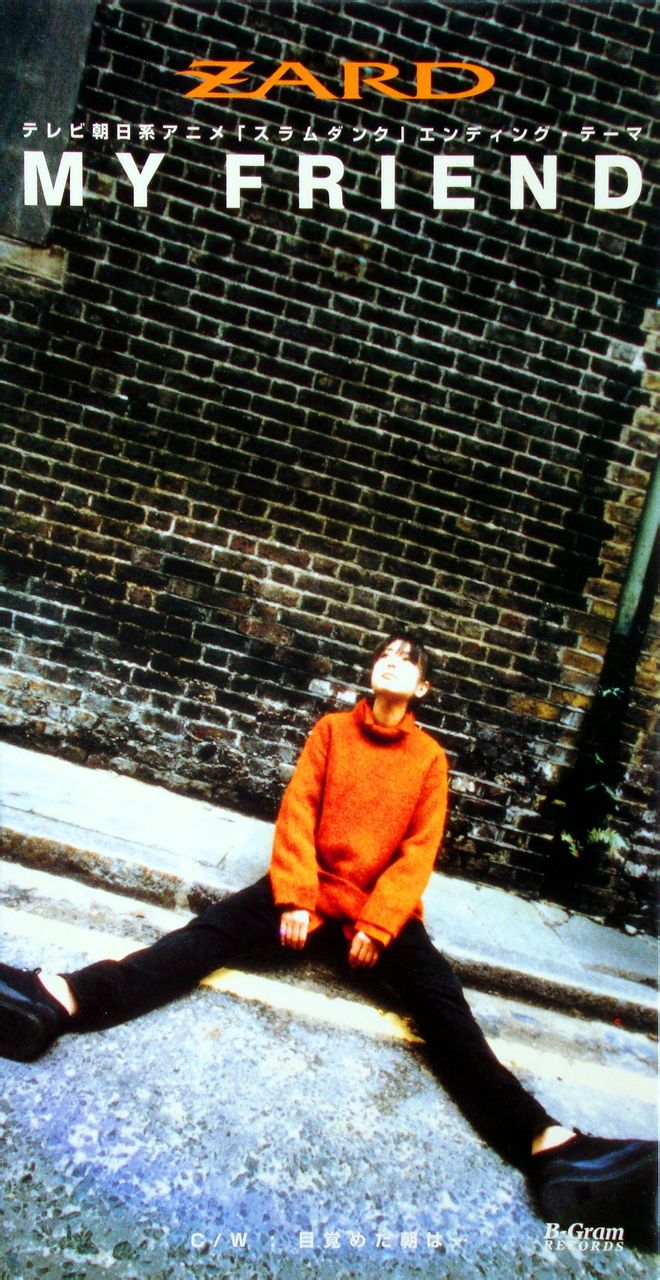
\includegraphics[width=0.3\textwidth]{S17.jpg}}

\large{

あなたを\ruby{想}{おも}うだけで 

心は\ruby{強}{つよ}くなれる 

ずっと\ruby{見}{み}つめているから 

\ruby{走}{はし}り\ruby{続}{つづ}けて 
\\

ひたむきだった\ruby{遠}{とおい}い\ruby{日}{ひ}の\ruby{夢}{ゆめ}は 

\ruby{今}{いま}でも\ruby{眩}{まぶ}しい 

どんなに\ruby{不安}{ふあん}がいっぱいでも 

\ruby{真}{ま}っすぐ\ruby{自分}{じぶん}の\ruby{道}{みち}を\ruby{信}{しん}じて 

\ruby{飾}{かざ}らない\ruby{素顔}{すがお}のあなたが\ruby{好}{す}き 

\ruby{変}{か}わってしまうことが\ruby{哀}{かな}しい 
\\

いつも\ruby{輝}{かがや}いていたね 

\ruby{少年}{しょうねん}のまま \ruby{瞳}{ひとみ}はMy Friend 

あなたがそばにいると 

\ruby{何故}{なぜ}か\ruby{素直}{すなお}になれた 

この\ruby{距離}{きょり}\ruby{通}{とお}り\ruby{抜}{ぬ}ける 

\ruby{風}{かぜ}になりたい 
\\

\ruby{真実}{ほんとう}の\ruby{愛}{あい}なら 

きっと\ruby{色}{いろ}んな\ruby{事}{こと} 

\ruby{乗}{の}り\ruby{越}{こ}えられたのに 

\ruby{涙}{ほし}のパレド 

\ruby{泪}{なみだ}がこぼれない\ruby{様}{よう}に 

\ruby{大}{おお}きく\ruby{息}{いき}を\ruby{吸}{す}った 

ひとりでいる\ruby{時}{とき}の\ruby{淋}{さび}しさより 

\ruby{二人}{ふたり}でいる\ruby{時}{とき}の\ruby{孤独}{こどく}の\ruby{方}{ほう}が\ruby{哀}{かな}しい 
\\

いつも\ruby{笑}{わら}っていたね 

あの\ruby{頃}{ころ}の\ruby{二人}{ふたり} 

せつないMy Friend 

あなたを\ruby{想}{おも}うだけで ど

\ruby{心}{こころ}は\ruby{強}{つよ}くなれる 

ずっと見つめているから 

\ruby{走}{はし}り\ruby{続}{つづ}けて 
\\

いつも\ruby{輝}{かがや}いていたね 

\ruby{少年}{しょうねん}のまま \ruby{瞳}{ひとみ}はMy Friend 

あなたを\ruby{想}{おも}うだけで 

\ruby{心}{こころ}は\ruby{強}{つよ}くなれる 

ずっと見つめているから 

\ruby{走}{はし}り\ruby{続}{つづ}けて 
\\

\ruby{走}{はし}り\ruby{続}{つづ}けて...

}

\hypertarget{7_1}{}
\section{ 君がいたから}
\large{

\ruby{抑}{おさ}えきれない\ruby{想}{おも}いや

\ruby{人}{ひと}が\ruby{泣}{な}いたり \ruby{惱}{なや}んだりすることは

\ruby{生}{い}きてる\ruby{証拠}{しょうこ}だね

\ruby{笑}{わら}いたい\ruby{奴}{やつ}らには \ruby{笑}{わら}わせておけばいいさ

\ruby{僕}{ぼく}らは\ruby{風}{かぜ}に\ruby{吹}{ふ}かれよう
\\

\ruby{感}{かん}じ\ruby{合}{あ}えば すべてがわかる

\ruby{言葉}{ことば}はなくても

\ruby{何度}{なんど}もくじけそうになって

ここまで\ruby{来}{き}たんだ

Oh \ruby{今}{いま} \ruby{僕}{ぼく}らの\ruby{心}{こころ}はひとつになる

\ruby{振}{ふ}り\ruby{向}{む}けば いつも \ruby{君}{きみ}がいたから
\\

\ruby{ドア}{Door}を\ruby{開}{あ}けて\ruby{中}{なか}に\ruby{入}{はい}ろうとしても

\ruby{入口}{いりぐち}が\ruby{見}{み}つからなくて

\ruby{誰}{だれ}かを\ruby{傷}{きず}つけた…

そんな\ruby{時}{とき} \ruby{友達}{ひと}が\ruby{自分}{じぶん}より\ruby{偉}{えら}く\ruby{見}{み}えたよ

\ruby{僕}{ぼく}はちっぽけな\ruby{存在}{やつ}だった
\\

まるで\ruby{鳥}{とり}になったみたいに

\ruby{自由}{じゆう}にはばたくよ

\ruby{何}{なに}が\ruby{正}{ただ}しい…

\ruby{何}{なに}が\ruby{間違}{まちが}っているのかなんて…

Oh \ruby{大勢}{なかま}の\ruby{中}{なか}に\ruby{居}{い}ても \ruby{孤独}{こどく}を\ruby{感}{かん}じていた

\ruby{目}{め}を\ruby{閉}{と}じると そこに \ruby{君}{きみ}がいたから
\\

\ruby{輝}{かがや}く\ruby{季節}{とき}の\ruby{中}{なか}で \ruby{夢}{ゆめ}は

\ruby{藍}{あお}く\ruby{染}{そ}まるだろう

\ruby{失}{うしな}うものは\ruby{何}{なに}ひとつない

\ruby{愛}{あい}さえあれば

Oh この\ruby{世界}{せかい}に \ruby{踊}{おど}り\ruby{続}{つづ}けるしかないのか

\ruby{心}{こころ}の\ruby{中}{なか}に \ruby{君}{きみ}がいたから

}

\hypertarget{7_2}{}
\section{ サヨナラは今もこの胸に居ます}

\parpic[r]{
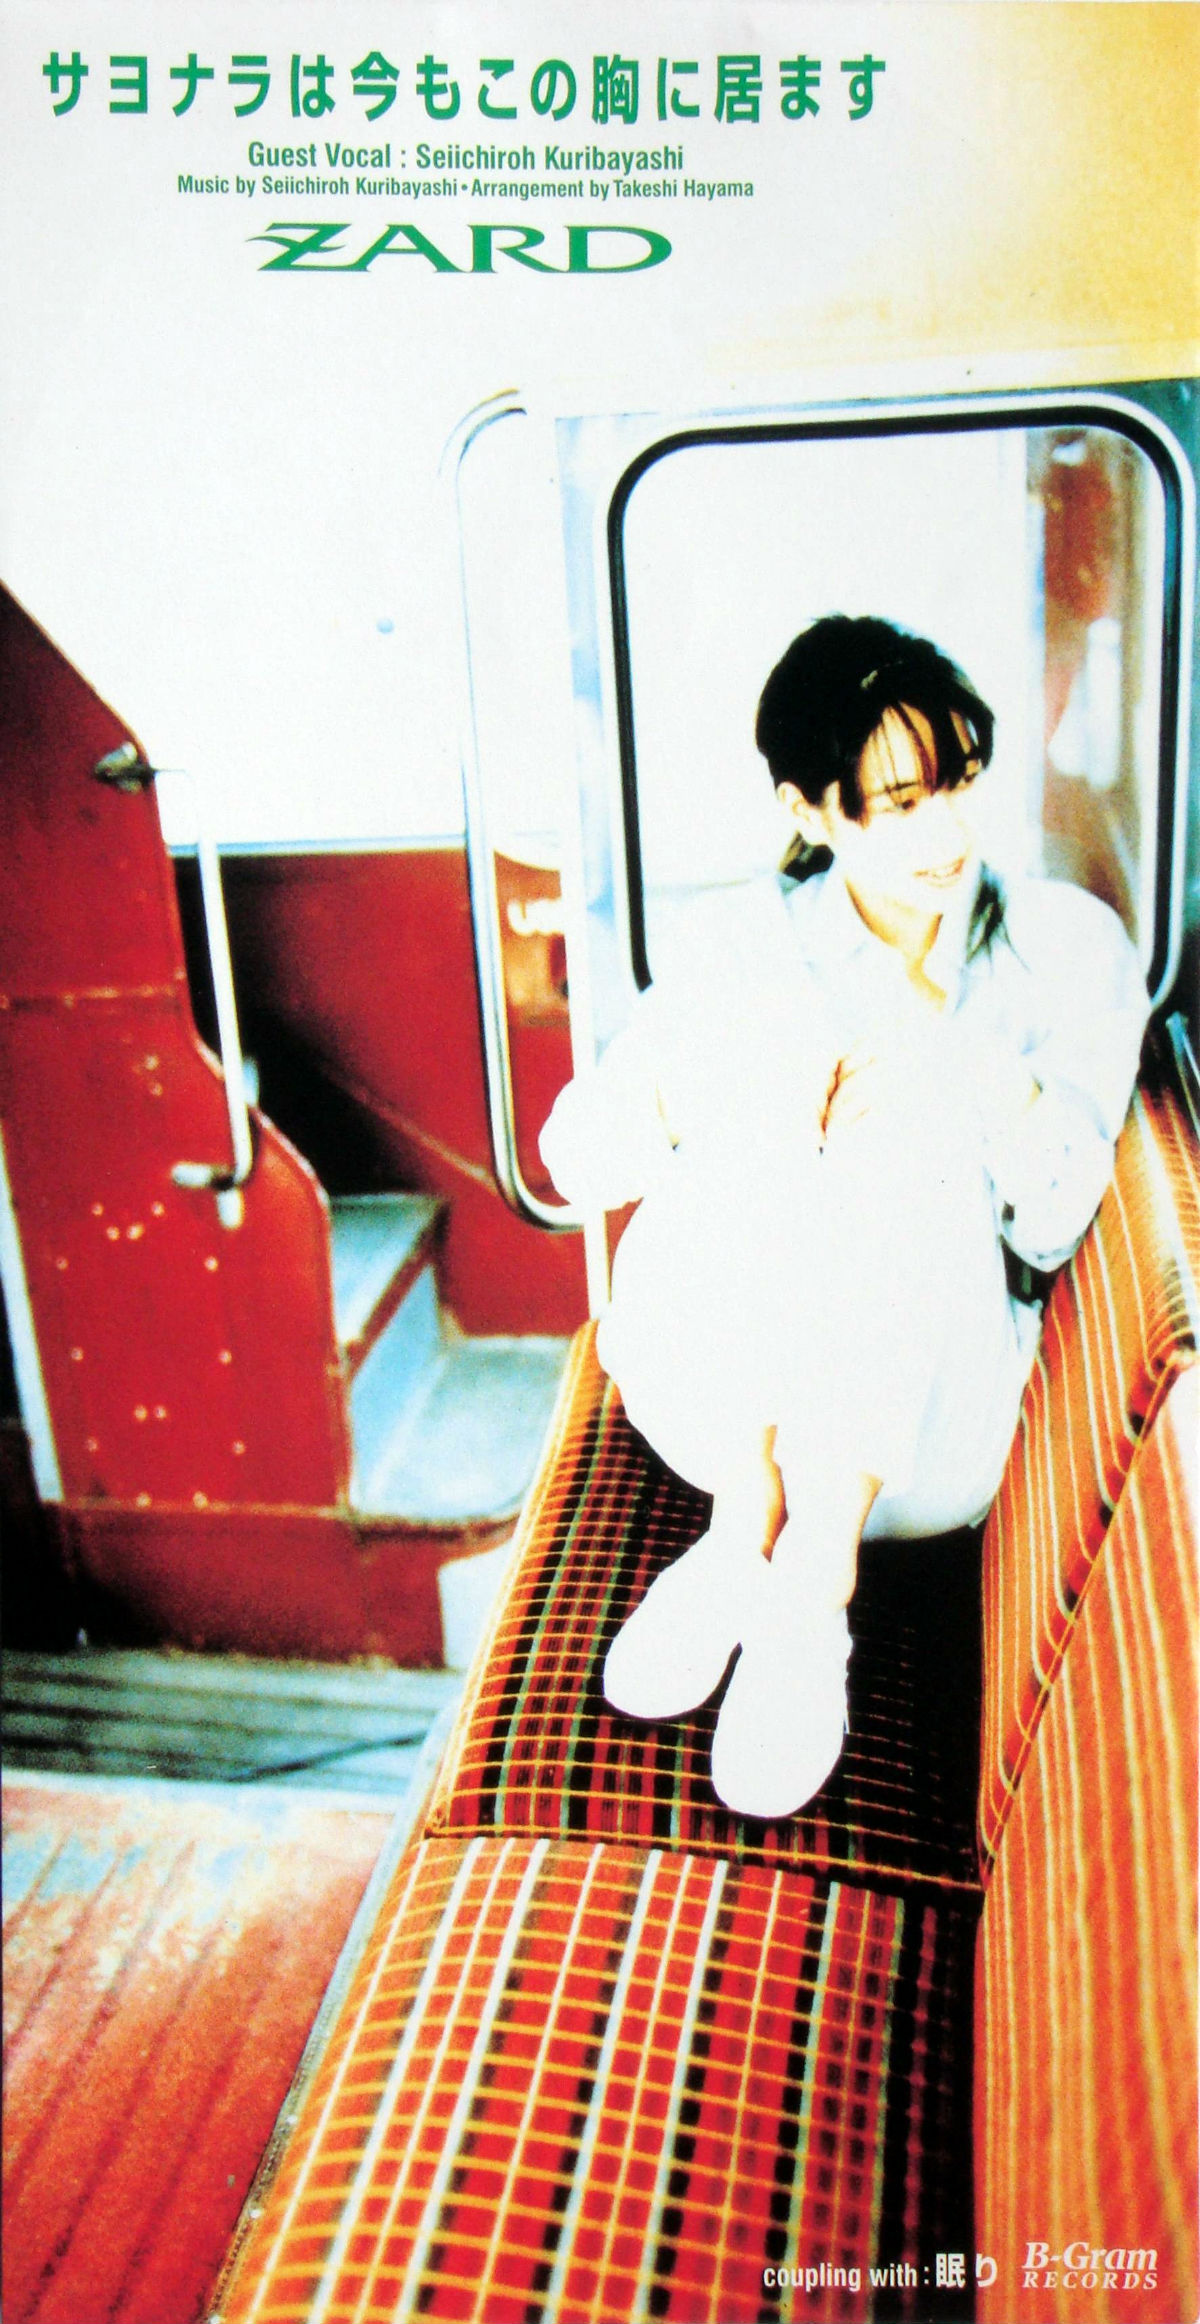
\includegraphics[width=0.3\textwidth]{S16.jpg}}

\large{

\ruby{地下鉄}{ちかてつ}の\ruby{駅}{えき}ひとつ\ruby{乗}{の}りすごし

\ruby{見慣}{みな}れた\ruby{街}{まち}を\ruby{横切}{よこぎ}ったら

\ruby{星空}{ほしぞら}を\ruby{数}{かぞ}える\ruby{頃}{ころ}あなたの\ruby{部屋}{へや}に\ruby{明}{あ}かりが…

もし あなたがいつか\ruby{独}{ひと}りになって

\ruby{私}{わたし}の\ruby{事}{こと}を\ruby{思}{おも}い\ruby{出}{だ}したら すぐに\ruby{連絡}{れんらく}してね

\ruby{好}{す}きだから\ruby{追}{お}わないと\ruby{心}{こころ}に\ruby{決}{き}めたの
\\

サヨナラは\ruby{今}{いま}もこの\ruby{胸}{むね}に\ruby{居}{い}ます

\ruby{出逢}{であ}った\ruby{頃}{ころ}の\ruby{私}{わたし}でいたい

あなたと\ruby{歩}{ある}いた\ruby{思}{おも}い\ruby{出}{で}の\ruby{中}{なか}を

\ruby{今}{いま}はひとり あの\ruby{道}{みち}をたどっています
\\

\ruby{久}{ひさ}しぶりにこんなに\ruby{笑}{わら}った

\ruby{笑}{わら}うことさえ\ruby{忘}{わす}れていた

\ruby{誰}{だれ}かに\ruby{必要}{ひつよう}とされたいから

\ruby{誰}{だれ}かの\ruby{為}{ため}に\ruby{ガンバ}{Gamba}ってる
\\

サヨナラは\ruby{今}{いま}もこの\ruby{胸}{むね}に\ruby{居}{い}ます

いつも\ruby{笑顔}{えがお}でかくしていたけど

\ruby{夏}{なつ}が\ruby{過}{す}ぎるたび この\ruby{胸}{むね}が\ruby{痛}{いた}い

\ruby{夜}{よる}はとても とても\ruby{長}{なが}く\ruby{感}{かん}じるのです
\\

サヨナラは\ruby{今}{いま}もこの\ruby{胸}{むね}に\ruby{居}{い}ます

\ruby{出逢}{であ}った\ruby{頃}{ころ}の\ruby{私}{わたし}でいたい

\ruby{楽}{たの}しかった\ruby{事}{こと} \ruby{苦}{くる}しかった\ruby{事}{こと}

そしていつの\ruby{日}{ひ}かあなたから\ruby{卒業}{そつぎょう}します

}

\hypertarget{7_3}{}
\section{ Love ~眠れずに君の横顔ずっと見ていた~}
\large{

\ruby{明日}{あした}も\ruby{一日}{いちにち}  \ruby{謙虛}{けんきょ}を\ruby{裝}{そ}って

\ruby{他人}{ひと}に\ruby{調子}{ちょし}を\ruby{合}{あ}わせ

「バランスがいい」と\ruby{譽}{ほ}められては  \ruby{自分}{じぶん}を\ruby{見失}{みうしな}う

\ruby{景氣}{けしき}のいい\ruby{話}{はなし}ばかり\ruby{求}{もと}め

\ruby{好成績}{こうせいせき}を\ruby{上}{あ}げたとしても

\ruby{用}{よう}が\ruby{終}{お}われば  \ruby{捨}{ばす}てられる  ボロボロのダンボール
\\

ドアを\ruby{開}{あけ}け  \ruby{風}{かぜ}を\ruby{入}{い}れよう

\ruby{街}{まち}は\ruby{無防備}{むぼうび}に\ruby{眠}{ねむ}っている  break around
\\

LOVE  \ruby{眠}{ねむ}れずに  \ruby{君}{きみ}の\ruby{橫顏}{よこがお}  ずっと\ruby{見}{み}ていた

いつの\ruby{日}{ひ}か\ruby{時}{とき}を\ruby{止}{と}めて  \ruby{思}{おも}いっきり\ruby{愛}{あい}したいよ 

 \ruby{体}{からだ}じゅう\ruby{時代}{じだい}の\ruby{速}{はや}さに  \ruby{遲}{おく}れてもいいよね

\ruby{不器用}{ぶきよう}でも  \ruby{君}{きみ}と\ruby{生}{い}きてゆきたい
\\

\ruby{三年前}{さんえんまえ}に  よく\ruby{著}{き}ていた\ruby{服}{ふく}を

久しぶりに\ruby{著}{き}てみたら

しょうのうと\ruby{二人}{ふたり}の  \ruby{思}{おも}い\ruby{出}{で}の\ruby{勾}{にお}いがした

あの\ruby{頃}{ころ}  いつも\ruby{話}{はなし}あっては\ruby{決}{き}めてたルールって\ruby{何}{あん}だったの?

\ruby{將來}{しょうらい}の\ruby{青寫真}{あおじゃしん}  いつしか\ruby{白紙}{はくし}になる
\\

\ruby{新}{あ}しいスタートに\ruby{向}{む}かって\ruby{張}{は}り\ruby{切}{はり}ってる\ruby{仲間}{なかま}を

\ruby{遠}{とお}く\ruby{感}{かん}じる  break around
\\

LOVE  \ruby{眠}{ねむ}れずに  \ruby{君}{きみ}の\ruby{橫顏}{よこがお}  ずっと\ruby{見}{み}ていた

いつの\ruby{日}{ひ}か\ruby{時}{とき}を\ruby{止}{と}めて  \ruby{思}{おも}いっきり\ruby{愛}{あい}したいよ  \ruby{体}{からだ}じゅう

\ruby{時代}{じだい}の\ruby{流}{はや}れに  \ruby{溺}{おく}れてもいいよね

\ruby{不器用}{ぶきよう}でも  \ruby{君}{きみ}と\ruby{生}{い}きてゆきたい

}

\hypertarget{7_4}{}
\section{ DAN DAN 心魅かれてく}
\large{

DAN DAN \ruby{心魅}{こころひ}かれてく その\ruby{眩}{まぶ}しい\ruby{笑顔}{えがお}に

\ruby{果}{は}てない\ruby{闇}{やみ}から\ruby{飛}{と}び\ruby{出}{だ}そう Hold My Hand
\\

\ruby{君}{きみ}とであったとき 

\ruby{子供}{こど}の\ruby{頃}{ころ}\ruby{大切}{たいせつ}に

\ruby{思}{おも}っていた 

\ruby{場所}{ばしょ}を\ruby{思}{おも}い\ruby{出}{だ}したんだ

\ruby{僕}{ぼく}と\ruby{踊}{おど}ってくれないか 

\ruby{光}{ひかに}と\ruby{影}{かげ}のWinding Road

\ruby{今}{いま}でもあいつに\ruby{夢中}{むちゅう}なの

\ruby{少}{すこ}しだけ\ruby{振}{ふ}り\ruby{向}{む}きたくなる 

ような\ruby{時}{とき}も\ruby{歩}{ある}けど

\ruby{愛}{あい}と\ruby{勇気}{ゆうき}と\ruby{誇}{ほこ}りを\ruby{持}{も}って\ruby{戦}{たたか}うよ
\\

DAN DAN \ruby{心魅}{こころひ}かれてく 

この\ruby{星}{ほし}の\ruby{希望}{きぼう}のかけら

きっと\ruby{誰}{だれ}もが\ruby{永遠}{えいえん}に\ruby{手}{て}にいれたい

ZEN ZEN 

\ruby{気}{き}にしない\ruby{振}{ふ}りしても 

ほら\ruby{君}{きみ}に\ruby{恋}{こい}してる

\ruby{果}{は}てない\ruby{闇}{やみ}から\ruby{飛}{と}び\ruby{出}{だ}そう 

Hold Your Hand
\\

\ruby{起}{お}こった\ruby{顔}{か}も\ruby{疲}{つか}れてる 

\ruby{君}{きみ}も\ruby{好}{す}きだけど

あんなに\ruby{飛}{と}びして\ruby{生}{い}きて 

\ruby{大丈夫}{だいじょうぶ}かなと\ruby{思}{おも}う

\ruby{僕}{ぼく}は\ruby{何気}{なにげ}ないしぐさに 

\ruby{降}{ふ}り\ruby{間}{ま}はされてる Sea Side Blue

それでもあいつに\ruby{夢中}{むちゅう}なの

もっと\ruby{聞}{き}きたいことがあったのに 

\ruby{二人}{ふたり}の\ruby{会話}{かいわ}が

\ruby{車}{くるま}の\ruby{音}{おと}に\ruby{阻}{はば}まれて 

\ruby{通}{とう}りにまうよ
\\

DAN DAN \ruby{心魅}{こころひ}かれてく 

\ruby{自分}{じぶん}でも\ruby{不思議}{ふしぎ}なんだけど

\ruby{何}{なん}かあると\ruby{直}{す}ぐに\ruby{君}{きみ}に\ruby{電話}{でんわ}したくなる

ZEN ZEN 

\ruby{気}{き}のない\ruby{振}{ふ}りしても

\ruby{結局}{けっきょく}\ruby{君}{きみ}のことだけ\ruby{見}{み}ていた

\ruby{海}{うみ}のかなたえ\ruby{飛}{と}び\ruby{出}{だ}そうよ 

Hold My Hand

}

\hypertarget{7_5}{}
\section{ 眠り}
\large{

\ruby{淋}{さび}しさに\ruby{戦}{たたか}う\ruby{夜}{よる}には

\ruby{誰}{だれ}かの\ruby{声}{こえ}が\ruby{聽}{き}きたくて

\ruby{手帳}{てちょ}を\ruby{見}{み}ても\ruby{誰}{だれ}にも\ruby{電話}{でんわ}するところがないし

なんとなくテレビをつけても

むなしい\ruby{気持}{きも}ちが\ruby{広}{ひろ}がって

\ruby{誰}{だれ}かにたった\ruby{一人}{ひとり}でいいから

いつも\ruby{気}{き}にかけていてほしい
\\

そんな\ruby{夜}{よる}はお\ruby{風呂}{ふろ}にひざをかかえて\ruby{入}{はい}り

\ruby{色々}{いろいろ}な\ruby{事}{こと}を

\ruby{子供}{こども}の\ruby{時}{とき}の\ruby{事}{こと}や

\ruby{学生}{がくせい}\ruby{時代}{じだい}の\ruby{事}{こと}
\\

そして\ruby{昔}{むかし}\ruby{好}{す}きだった

あの\ruby{人}{ひと}の\ruby{事}{こと}を\ruby{思}{おも}い\ruby{出}{だ}す

そうしているうちに\ruby{眠}{ねむ}りが

やさしく\ruby{私}{わたし}を\ruby{誘}{さそ}う
\\

ねぇ \ruby{友達}{ともだち}に

\ruby{裏切}{うらぎ}られた\ruby{事}{こと}ってない?

\ruby{土足}{どそく}で\ruby{心}{こころ}に\ruby{踏}{ふ}みこんだこと

きって\ruby{気}{き}づいてない
\\

だから\ruby{昔}{むかし}\ruby{好}{す}きだった

あの\ruby{人}{ひと}の\ruby{事}{こと}を\ruby{思}{おも}い\ruby{出}{だ}す

そうしているうちに\ruby{眠}{ねむ}りが

やさしく\ruby{私}{わたし}を\ruby{誘}{さそ}う
\\

\ruby{眠}{ねむ}れる\ruby{事}{こと}が\ruby{嬉}{うれ}しい

\ruby{時計}{とき}が遠くで\ruby{聞}{き}こえる

}

\hypertarget{7_6}{}
\section{ 心を開いて}

\large{

\ruby{私}{わたし}はあなたが\ruby{想}{おも}ってる\ruby{様}{よう}な\ruby{人}{ひと}では

ないかもしれない

でも\ruby{不思議}{ふしぎ}なんだけど

あなたの\ruby{声}{こえ}を\ruby{聞}{き}いてると

とても \ruby{優}{やさ}しい\ruby{気持}{きも}ちになるのよ
\\

このままずっと \ruby{忘}{わす}れたくない

\ruby{現実}{いま}が\ruby{想}{おも}い\ruby{出}{で}に\ruby{変}{か}わっても

\ruby{言葉}{ことば}はないけど きっとあなたも

\ruby{同}{おな}じ\ruby{気持}{きも}ちでいるよね
\\

\parpic[r]{
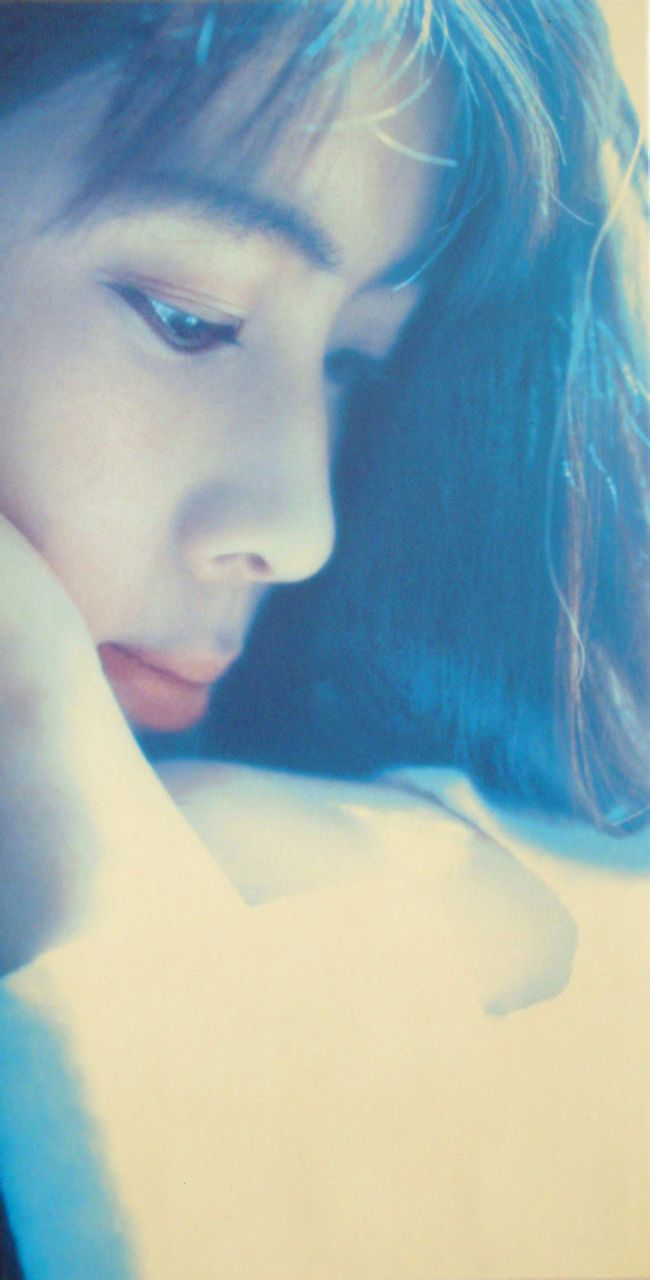
\includegraphics[width=0.3\textwidth]{S18.jpg}}

\ruby{人}{ひと}と\ruby{深}{ふか}くつきあうこと

\ruby{私}{わたし}もそんなに\ruby{得意}{とくい}じゃなかった

でも あなたを\ruby{見}{み}ていると

\ruby{私}{わたし}と\ruby{似}{に}ていて もどかしい

そういう\ruby{所}{ところ}が たまらなく\ruby{好}{す}きなの
\\

ビルの\ruby{隙間}{すきま}に\ruby{二人}{ふたり}\ruby{座}{すわ}って

\ruby{道}{みち}\ruby{行}{い}く\ruby{人}{ひと}を ただ\ruby{眺}{なが}めていた

\ruby{時間}{ときかん}が\ruby{過}{す}ぎるのが \ruby{悲}{かな}しくて

あなたの\ruby{肩}{かた}に\ruby{寄}{よ}りそった
\\

My dream Your smile

\ruby{忘}{わす}れようとすればする\ruby{程}{ほど} \ruby{好}{す}きになる

それが\ruby{誤解}{ごかい}や\ruby{錯覚}{さっかく}でも…

\ruby{心}{こころ}を\ruby{開}{ひら}いて
\\

どんなときも あなたの\ruby{胸}{むね}に

\ruby{迷}{まよ}わず\ruby{飛}{と}び\ruby{込}{こ}んでゆくわ

Your dream I believe

ときめいてる \ruby{心}{こころ}を\ruby{開}{ひら}いて

}

\hypertarget{7_7}{}
\section{ 突然}
\large{

\ruby{突然}{とつぜん}\ruby{君}{きみ}からの\ruby{手紙}{てがみ}

あの\ruby{日}{ひ}から\ruby{途切}{とぎ}れた\ruby{君}{きみ}の\ruby{声}{こえ}

\ruby{今}{いま}すぐ\ruby{逢}{あ}いに\ruby{行}{ゆ}くよ

\ruby{夏}{なつ}が\ruby{遠回}{とおまわ}りしても
\\

\parpic[r]{
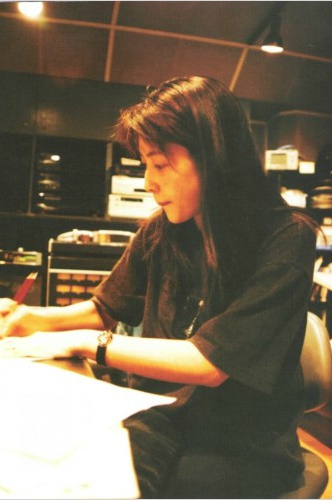
\includegraphics[width=0.3\textwidth]{F1.jpg}}

\ruby{カセット}{cassette}の\ruby{ボリューム}{volume}\ruby{上}{あ}げた

\ruby{日曜}{にちよう}の\ruby{車}{くるま}は\ruby{混}{まじ}んでいる

\ruby{バックミラー}{back mirror}の\ruby{自分}{じぶん}を\ruby{見}{み}て

「\ruby{今度}{こんど}こそは\ruby{意地}{いじ}を\ruby{張}{は}らない…」

\ruby{海岸通}{かいがんどお}り\ruby{過}{す}ぎると

\ruby{君}{きみ}の\ruby{家}{いえ}が\ruby{見}{み}える

\ruby{過去}{かこ}も\ruby{未来}{みらい}も\ruby{忘}{わす}れて

\ruby{現在}{いま}は\ruby{君}{きみ}のことだけ
\\

\ruby{突然}{とつぜん}の\ruby{風}{かぜ}に\ruby{吹}{ふ}かれて

\ruby{夢中}{むちゅう}で\ruby{何}{なに}かを\ruby{探}{さが}したね

\ruby{倒}{たお}れそうになったら

\ruby{僕}{ぼく}を\ruby{近}{ちか}くに\ruby{感}{かん}じて

またあの\ruby{日}{ひ}のように\ruby{君}{きみ}を\ruby{抱}{だ}きしめたい
\\

\ruby{何}{なに}かを\ruby{求}{もと}めれば\ruby{何}{なに}かが

\ruby{音}{おと}をたてて\ruby{崩}{くず}れてく

たとえ\ruby{今日}{きょう}が\ruby{終}{お}わっても

\ruby{明日}{あした}を\ruby{信}{しん}じて行こうよ

\ruby{僕}{ぼく}は\ruby{君}{きみ}の\ruby{大事}{だいじ}な

\ruby{存在}{ひと}になれるのだろうか

この\ruby{仕事}{ゆめ}はどんな\ruby{状況}{とき}も

\ruby{笑}{わら}っているよ
\\

\ruby{突然}{とつぜん}の\ruby{熱}{あつ}い\ruby{夕立}{ゆうだ}ちに

\ruby{夢中}{むちゅう}で\ruby{車}{くるま}に\ruby{走}{はし}ったね

\ruby{埃}{ほこり}まみれになって

\ruby{時間}{とき}の\ruby{経}{た}つのも\ruby{忘}{わす}れた

\ruby{恋人}{こいびと}よ\ruby{君}{きみ}を\ruby{心}{こころ}から

\ruby{大切}{たいせつ}にしたい
\\

\ruby{突然}{とつぜん}の\ruby{風}{かぜ}に\ruby{吹}{ふ}かれて

\ruby{旅人}{たびびと}は\ruby{行}{ゆ}く\ruby{先}{さき}を\ruby{知}{し}らない

でも\ruby{僕}{ぼく}らの\ruby{愛}{あい}は

\ruby{二度}{にど}とはぐれたりはしない

あの\ruby{青}{あお}い\ruby{空}{そら}のように

いつまでもそばにいる

}

\hypertarget{7_8}{}
\section{ 今日も}
\large{

こんな\ruby{風}{ふう}にしかられたの はじめて

つい「\ruby{別}{わか}れたい」と\ruby{云}{い}った

「\ruby{何故}{なぜ}もっと\ruby{素直}{すなお}に\ruby{話}{はなし}を\ruby{聞}{き}こうとしないんだ」と

\ruby{言}{い}い\ruby{殘}{のこ}して
\\

\ruby{冷}{さ}めてる\ruby{感}{かん}じって \ruby{相手}{あいて}にも\ruby{伝}{つた}わるの

\ruby{偶然}{ぐうぜん}の\ruby{電話}{でんわ}から \ruby{聽}{き}こえてしまった\ruby{声}{こえ}

\ruby{彼}{かれ}が\ruby{帰}{かえ}ったあとの \ruby{冷}{つめ}たく\ruby{響}{ひび}いた\ruby{ドア}{door}

うしろ\ruby{姿}{すがた}は \ruby{今日}{きょう}も とても\ruby{疲}{つか}れていた
\\

\ruby{今頃}{いまごろ} \ruby{見知}{みし}らぬあの\ruby{彼女}{ひと}と

\ruby{背中}{せなか}を\ruby{向}{む}けて\ruby{眠}{ねむ}っているの?

それとも\ruby{二人}{ふたり} \ruby{別々}{べつべつ}の\ruby{寢室}{へや}で

ひとり\ruby{目}{め}を\ruby{覚}{さ}ますの?
\\

もうそんな\ruby{事}{こと} \ruby{考}{かんが}えるのは\ruby{止}{よ}そう

あなたの\ruby{気持}{きも}ちが そう\ruby{痛}{いた}い\ruby{程}{ほど}わかるから

\ruby{今}{いま}が\ruby{楽}{たの}しければ\ruby{楽}{たの}しい\ruby{程}{ほど}

いつか\ruby{来}{く}る わかれの\ruby{時}{とき}が つらくなるけれど
\\

あなたとの\ruby{事}{こと}は \ruby{友達}{ともだち}に\ruby{話}{はな}せない

\ruby{話}{はな}したら\ruby{嫌}{きら}われそうで

うまく\ruby{弁解}{いいわけ}もできそうにない

\ruby{明日}{あした}になったら \ruby{嫌}{きら}いになれるのかな

でも\ruby{本当}{ほんとう}に\ruby{叱}{しか}れってくれるのは

あなただけだから
\\

\ruby{今日}{きょう}も あなたのことが いちばん\ruby{好}{す}きでした

}

\hypertarget{7_9}{}
\section{ Today is another day}
\large{

かわいくなれない ほんとうの\ruby{理由}{わけ}は

あなたが \ruby{私}{わたし}を\ruby{選}{えら}ばないって

\ruby{知}{し}っているから

きき\ruby{覚}{おぼ}えのある \ruby{足音}{あしおと}がして

「あっ」と\ruby{振}{ふ}り\ruby{返}{かえ}ったら \ruby{人違}{ひとちが}いだった
\\

きっと\ruby{心}{こころ}が\ruby{淋}{さび}しいんだ

\ruby{他人}{ひと}に\ruby{期待}{きたい}したい

あてにしたい \ruby{信}{しん}じていたい

もしあなたを\ruby{忘}{わす}れられたら

それでも\ruby{私}{わたし} \ruby{生}{い}きていけるのかな

\ruby{明日}{あした}がある
\\

\ruby{口}{くち}がうまい\ruby{人}{ひと}だと \ruby{誰}{だれ}かにきいた

\ruby{目}{め}の\ruby{前}{まえ}のとっても\ruby{弱}{よわ}い\ruby{人}{ひと}は うそなの?

\ruby{疑}{うたが}いだしたら きりがないのにね

\ruby{バカ}{馬鹿}みたい それでもあなたの\ruby{夢}{ゆめ}を\ruby{見}{み}る
\\

きっと\ruby{心}{こころ}が\ruby{淋}{さび}しいんだ

\ruby{他人}{ひと}に\ruby{期待}{きたい}しない

あてにしない \ruby{信}{しん}じたくない

\ruby{悲}{かな}しい\ruby{現実}{げんじつ}をなげくより

\ruby{今}{いま} \ruby{何}{なに}ができるかを\ruby{考}{かんが}えよう

\ruby{今日}{きょう}が\ruby{変}{か}わる
\\

きっと\ruby{心}{こころ}が\ruby{淋}{さび}しいんだ

\ruby{他人}{ひと}に\ruby{期待}{きたい}しない

あてにしない \ruby{信}{しん}じたくない

\ruby{悲}{かな}しい\ruby{現実}{げんじつ}をなげくより

\ruby{今}{いま} \ruby{何}{なに}ができるかを\ruby{考}{かんが}えよう

\ruby{今日}{きょう}が\ruby{変}{か}わる
\\

Today is another day

}

\hypertarget{7_10}{}
\section{ 愛が見えない}

\parpic[r]{
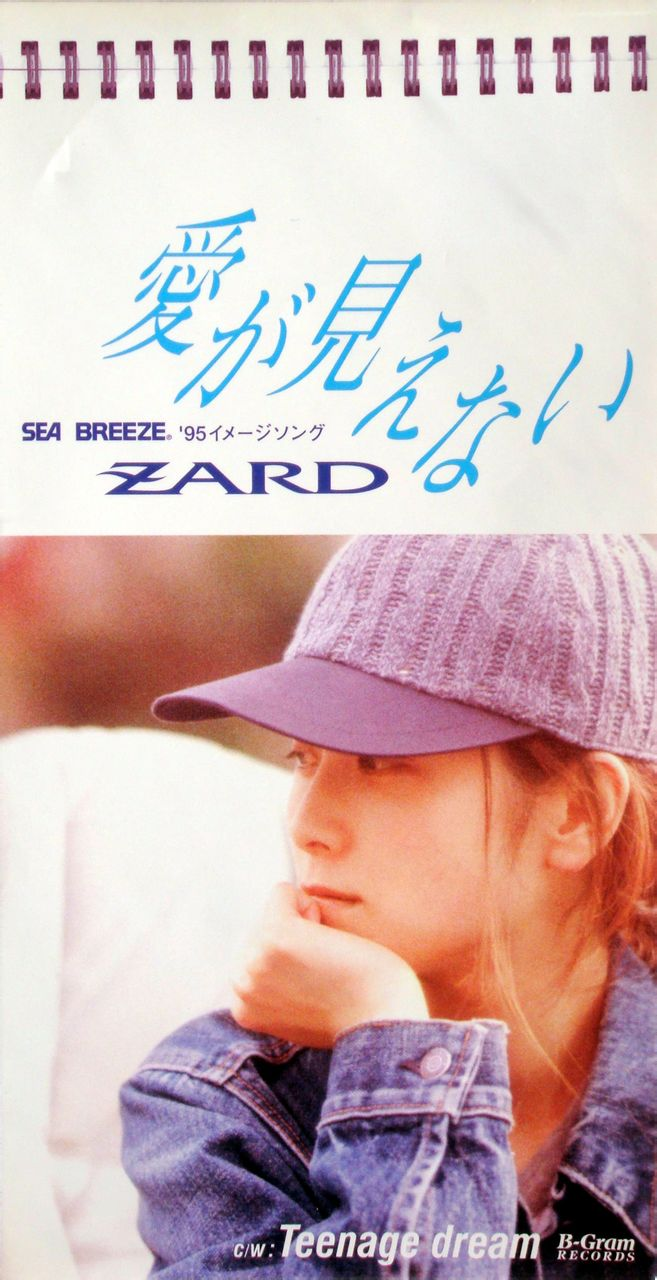
\includegraphics[width=0.3\textwidth]{S15.jpg}}

\large{

あの\ruby{頃}{ころ}は\ruby{楽}{たの}しかった 

\ruby{仲間}{なかま}も\ruby{多}{おお}くて

たわいもなく\ruby{何}{なに}\ruby{時間}{じかん}も\ruby{話}{はな}してた

\ruby{遊}{あそ}びの\ruby{帰}{かえ}り 

いつも\ruby{終電}{しゅうでん}に\ruby{乗}{の}り\ruby{遅}{おく}れたね

\ruby{懐}{なつ}かしいな 

あのドーナツ\ruby{屋}{Doughnutや}さん

\ruby{朝}{あさ}\ruby{一番}{いちばん}の\ruby{始発}{しはつ}で\ruby{帰}{かえ}る\ruby{私}{わたし}は 

ひどい\ruby{顔}{かお}

\ruby{出}{で}かけていく\ruby{時}{とき}の\ruby{私}{わたし}とは 

\ruby{別人}{べつじん}の\ruby{顔}{かお}

このごろ\ruby{逢}{あ}えばケンカばかり

\ruby{一緒}{いっしょ}に\ruby{居}{い}すぎかな
\\

\ruby{愛}{あい}が\ruby{見}{み}えない 

\ruby{今}{いま}の\ruby{時代}{じだい} \ruby{都会}{まち}はみんな 

\ruby{急}{いそ}ぎ\ruby{足}{あし}で

きっと\ruby{誰}{だれ}もが \ruby{孤独}{こどく}なのに 

あなたも\ruby{私}{わたし}も それを\ruby{見}{み}せない!
\\

\ruby{一人}{ひとり}で\ruby{生}{い}きて\ruby{行}{ゆ}くほど\ruby{強}{つよ}くないくせに

\ruby{時々}{ときどき} 

\ruby{独}{ひと}りになるのが\ruby{好}{す}きになる

\ruby{一番}{いちばん}\ruby{肝心}{かんじん}な\ruby{貴方}{ひと}に 

\ruby{何故}{なぜ}\ruby{優}{やさ}しくできないの?

\ruby{他}{ほか}の\ruby{人}{ひと}には\ruby{気}{き}を\ruby{使}{つか}うのに

\ruby{電話}{でんわ}を\ruby{切}{き}ったのはどっちが\ruby{先}{さき} 

\ruby{私}{わたし}が\ruby{先}{さき}

「もう\ruby{別}{わか}れよう」と\ruby{言}{い}い\ruby{出}{だ}したのは 

あなたが\ruby{先}{さき}

\ruby{夢}{ゆめ}を\ruby{捨}{す}てるのが\ruby{大人}{おとな}なら 

\ruby{大人}{おとな}になんかなりたくない
\\

\ruby{愛}{あい}が\ruby{見}{み}えない もうこれ\ruby{以上}{いじょう} 

あなたの\ruby{海}{うみ} \ruby{泳}{およ}げないわ

あんな\ruby{風}{ふう}にあなたの\ruby{事}{こと} 

\ruby{愛}{あい}せる\ruby{人}{ひと}は \ruby{私}{わたし}しかいない!
\\

\ruby{愛}{あい}が\ruby{見}{み}えない もうこれ\ruby{以上}{いじょう} 

あなたの\ruby{海}{うみ} \ruby{泳}{およ}げないわ

でも\ruby{私}{わたし}の \ruby{幸}{しあわ}せのカギ 

\ruby{握}{にぎ}っているのはあなたよ
\\

\ruby{愛}{あい}が\ruby{見}{み}えない Only you forever 

すべて\ruby{分}{わ}かりあえなくても

\ruby{言葉}{やさしさ}より \ruby{キス}{Kiss}が\ruby{欲}{ほ}しい 

\ruby{灼熱}{しゃくねつ}の\ruby{夏}{なつ}に\ruby{踊}{おど}らせて!

}

\hypertarget{7_11}{}
\section{ 見つめていたいね}
\large{

\ruby{帰}{かえ}りの\ruby{電車}{でんしゃ}は いつも \ruby{切}{せつ}なくなるのよ

\ruby{現在}{いま}どこにいるの \ruby{昨日}{きのう}\ruby{誰}{だれ}といたの

そんな\ruby{言葉}{ことば}で \ruby{縛}{しば}っていた

\ruby{今日}{きょう}の\ruby{態度}{たいど}が \ruby{許}{ゆる}せなくて

\ruby{無口}{むぐち}になったけど \ruby{後悔}{こうかい}してる

いつまでが\ruby{子供}{こども}で いつからが\ruby{大人}{おとな}なの?
\\

\ruby{見}{み}つめていたいね \ruby{出逢}{であ}った\ruby{頃}{ころ}を

そのまなざしに ドキドキしてた

\ruby{見}{み}つめていたいね あの\ruby{優}{やさ}しさを

\ruby{今}{いま}しか\ruby{出来}{でき}ない\ruby{事}{こと}を

\ruby{今}{いま} \ruby{感}{かん}じるままに
\\

\ruby{旅}{たび}の\ruby{途中}{とちゅう}で ちょっとひと\ruby{休}{やす}み

\ruby{肩}{かた}の\ruby{荷}{に}を おろしてしまおう

「3Gの\ruby{キーパー}{keeper}も \ruby{天国}{てんごく}から\ruby{見}{み}てる」

この\ruby{間}{あいだ}の\ruby{続}{つづ}きを \ruby{聞}{き}かせて
\\

あの\ruby{頃}{ころ}の\ruby{古}{ふる}い\ruby{車}{くるま}で \ruby{砂埃}{すなぼこ}りけって

\ruby{走}{はし}り\ruby{出}{だ}そう \ruby{太陽}{たいよう}の\ruby{街}{まち}へ

\ruby{ラジオ}{radio}の\ruby{ヴォリューム}{volume}あげて \ruby{人目}{ひとめ}\ruby{気}{き}にして

\ruby{昔}{むかし}みたいに \ruby{話}{はなし}が途切れたら \ruby{キス}{kiss}して
\\

\ruby{見}{み}つめていたいね \ruby{出逢}{であ}った\ruby{頃}{ころ}を

そのまなざしに ドキドキしてた

\ruby{見}{み}つめていたいね あの\ruby{優}{やさ}しさを

\ruby{今}{いま}しか\ruby{出来}{でき}ない\ruby{事}{こと}を

\ruby{今}{いま} \ruby{感}{かん}じるままに

}
{ \ }

{ \ }

{ \ }

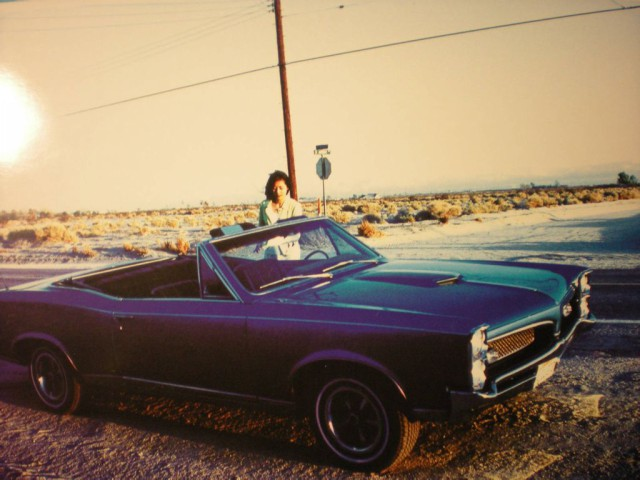
\includegraphics[width=0.9\textwidth]{P3.jpg}


\chapter{Album 8}
\thispagestyle{empty} %本页頁碼空白
\vspace{-16mm}
\LARGE {永遠}

\normalsize{JBCJ-1021 1999.2.17 \ release}
\\

\vspace{-5mm}

\parpic[l]{
\pichskip{6em}
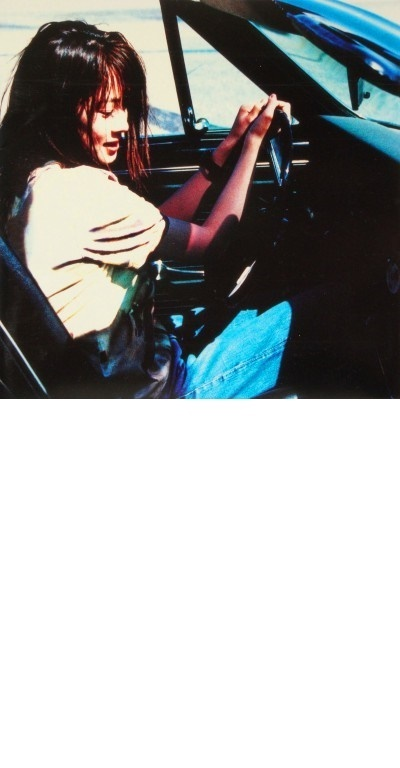
\includegraphics[width=0.4\textwidth]{8.jpg}}

\small{\hyperlink{8_0}{1.永遠}}

\tiny{作詞:坂井泉水 \ 作曲/編曲:徳永暁人}

\small{\hyperlink{8_1}{2.My Baby Grand ~ぬくもりが欲しくて~}}

\tiny{作詞:坂井泉水 \ 作曲:織田哲郎  \ 編曲:池田大介}

\small{\hyperlink{8_2}{3.WAKE UP MAKE THE MORNING LAST}}

\tiny{作詞:坂井泉水 \ 作曲:福山廣也  \ 編曲:古井弘人}

\small{\hyperlink{8_3}{4.Brand New Love}}

\tiny{作詞:坂井泉水 \ 作曲:綿貫正顕  \ 編曲:徳永暁人}

\small{\hyperlink{8_4}{5.運命のルーレット廻して}}

\tiny{作詞:坂井泉水 \ 作曲:栗林誠一郎  \ 編曲:池田大介}

\small{\hyperlink{8_5}{6.遠い星を数えて}}

\tiny{作詞:坂井泉水 \ 作曲:栗林誠一郎  \ 編曲:徳永暁人}

\small{\hyperlink{8_6}{7.新しいドア ~冬のひまわり~}}

\tiny{作詞:坂井泉水 \ 作曲:北野正人  \ 編曲:古井弘人}

\small{\hyperlink{8_7}{8.GOOD DAY}}

\tiny{作詞:坂井泉水 \ 作曲:綿貫正顕  \ 編曲:池田大介}

\small{\hyperlink{8_8}{9.I feel fine,yeah}}

\tiny{作詞:坂井泉水 \ 作曲:三好誠  \ 編曲:古井弘人}

\small{\hyperlink{8_9}{10.少女の頃に戻ったみたいに}}

\tiny{作詞:坂井泉水 \ 作曲:大野愛果  \ 編曲:池田大介}

\small{\hyperlink{8_10}{11.息もできない}}

\tiny{作詞:坂井泉水 \ 作曲:織田哲郎  \ 編曲:葉山たけし}

\small{\hyperlink{8_11}{12.風が通り抜ける街へ}}

\tiny{作詞:坂井泉水 \ 作曲:織田哲郎  \ 編曲:徳永暁人}

\small{\hyperlink{8_12}{13.フォトグラフ}}

\tiny{作詞:坂井泉水 \ 作曲/編曲:徳永暁人}

\clearpage


\hypertarget{8_0}{}
\section{ 永遠}

\parpic[r]{
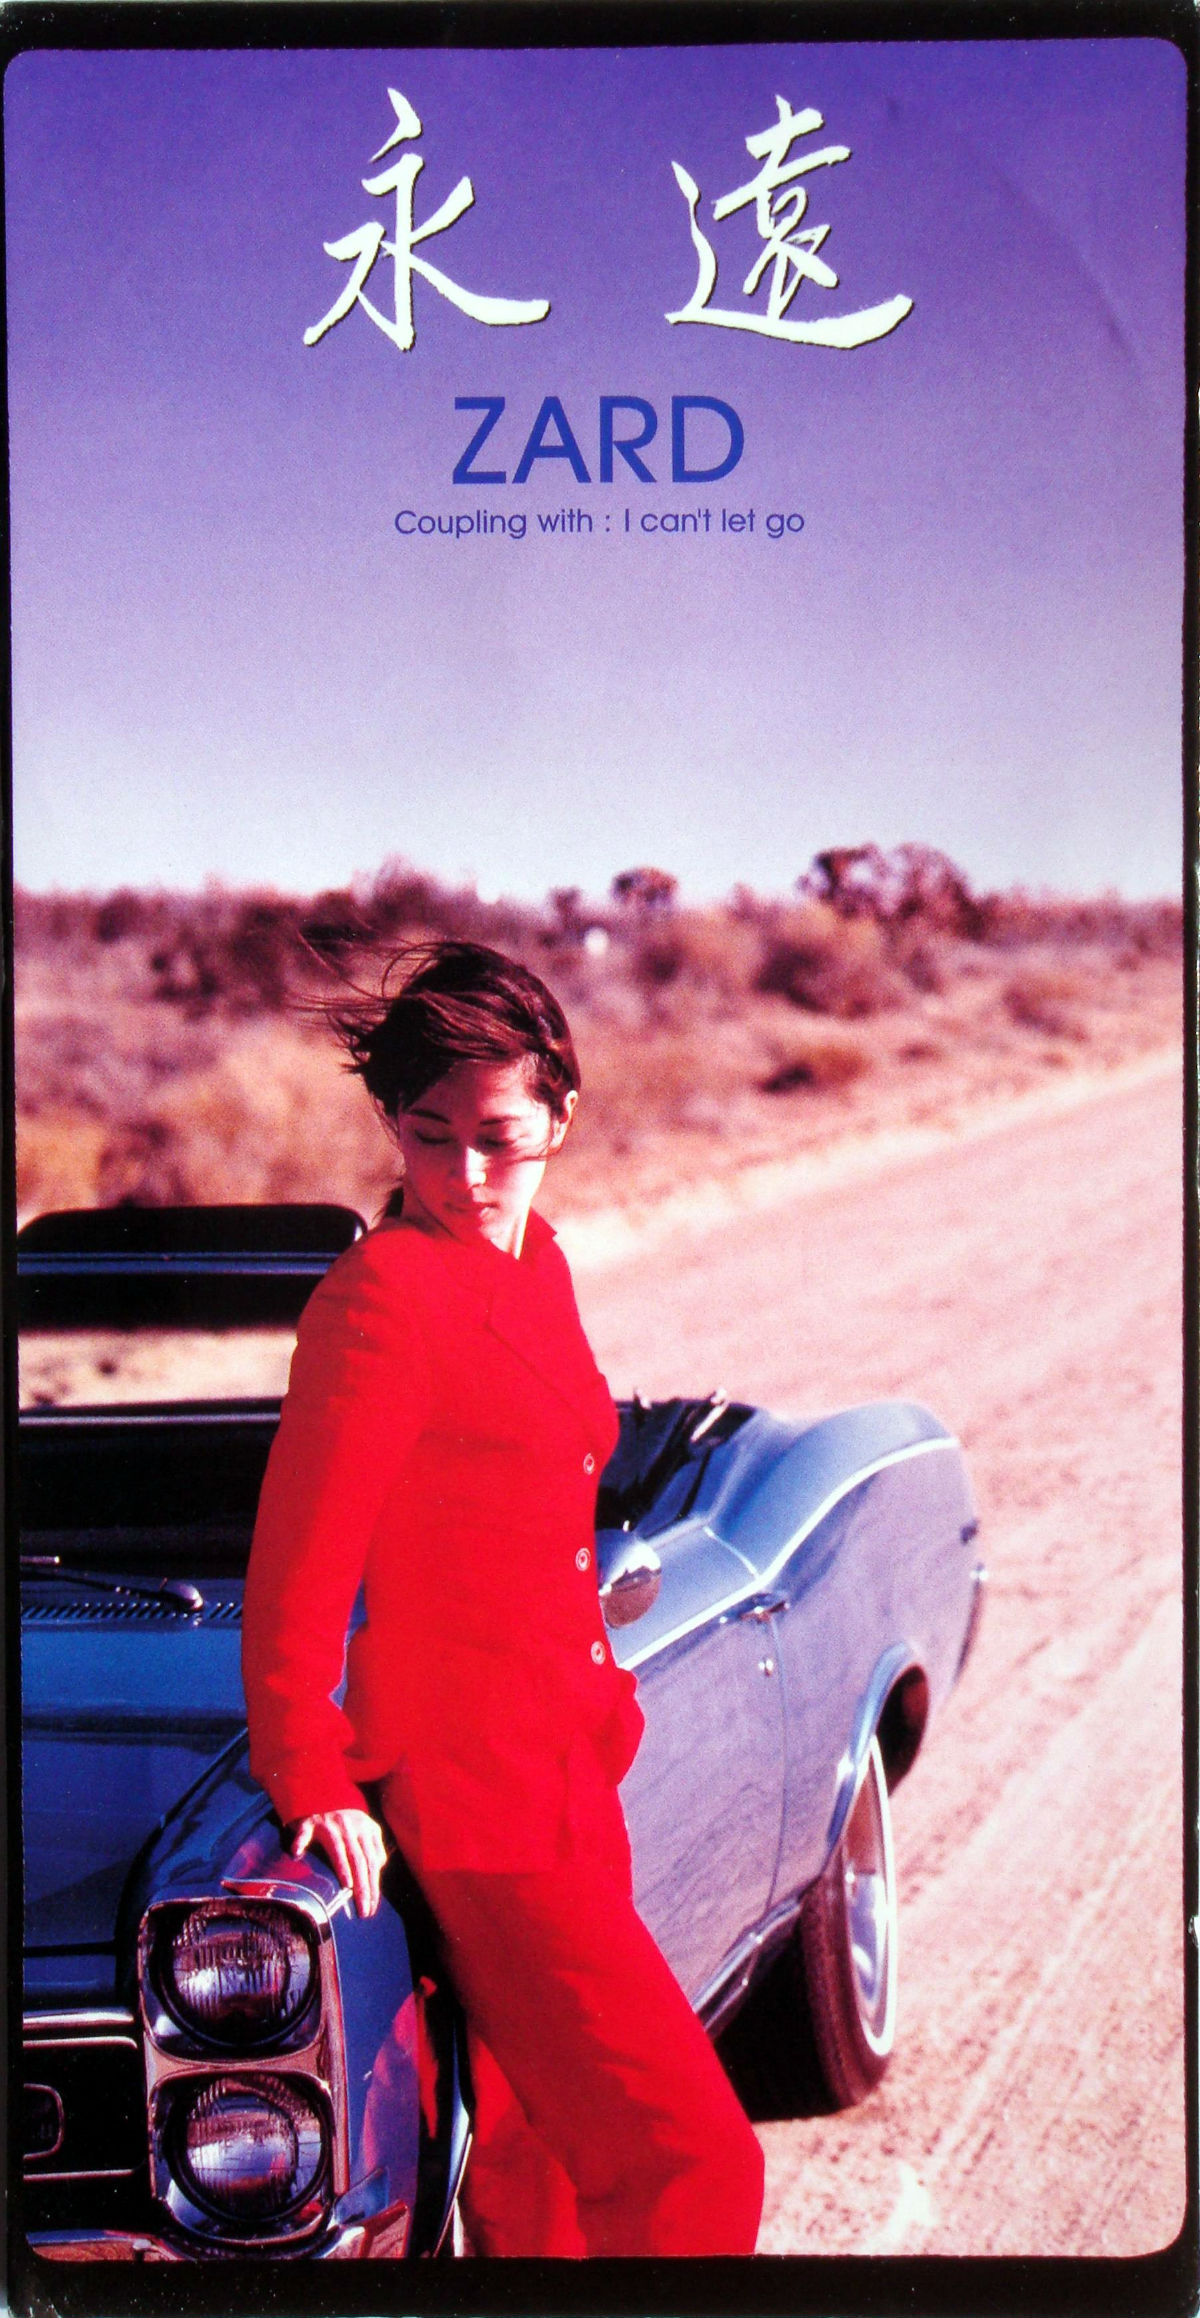
\includegraphics[width=0.3\textwidth]{S22.jpg}}

\large{

\ruby{朱}{あか}い\ruby{果実}{かじつ}を\ruby{見}{み}たら

\ruby{私}{わたし}のことを\ruby{思}{おも}い\ruby{出}{だ}してください

あなたの\ruby{決心}{けっしん}が\ruby{固}{かた}まったら…

きらきらと\ruby{ガラス}{Glass}の\ruby{粉}{かけら}になって

このまま \ruby{消}{き}えてしまいましょう 

\ruby{誰}{だれ}も\ruby{知}{し}らない\ruby{楽園}{くに}へ
\\

\ruby{今}{いま}の\ruby{二人}{ふたり}の\ruby{間}{あいだ}に 

\ruby{永遠}{えいえん}は\ruby{見}{み}えるのかな

すべてを \ruby{手}{て}に\ruby{入}{い}れることが \ruby{愛}{あい}ならば

もう\ruby{失}{うしな}うものなんて \ruby{何}{なに}も\ruby{怖}{こわ}くない
\\

\ruby{口}{くち}のきき\ruby{方}{かた}も\ruby{知}{し}らない 

\ruby{生意気}{なまいき}な\ruby{女性}{やつ}だと\ruby{思}{おも}った?

\ruby{偶然}{ぐうぜん} \ruby{街}{まち}で\ruby{見}{み}かけたけど 

\ruby{声}{こえ}をかけようかどうか\ruby{迷}{まよ}った

\ruby{守}{まも}るべきものは \ruby{何}{な}のか 

この\ruby{頃}{ころ} それが\ruby{分}{わ}からなくなる…
\\

「\ruby{君}{きみ}と\ruby{僕}{ぼく}との\ruby{間}{あいだ}に \ruby{永遠}{えいえん}は\ruby{見}{み}えるのかな」

どこまでも\ruby{続}{つづ}く\ruby{坂道}{さかみち}

あの\ruby{日}{ひ}から\ruby{淋}{さび}しかった 

\ruby{想像}{そうぞう}\ruby{以上}{いじょう}に… 

Just Fallin' of the Rain
\\

\ruby{君}{きみ}と\ruby{僕}{ぼく}との\ruby{間}{あいだ}に \ruby{永遠}{えいえん}は\ruby{見}{み}えるのかな

この\ruby{門}{もん}をくぐり\ruby{抜}{ぬ}けると

\ruby{安}{やす}らかなその\ruby{腕}{うで}にたどりつける

また\ruby{夢}{ゆめ}を\ruby{見}{み}る\ruby{日}{ひ}まで

}

\hypertarget{8_1}{}
\section{ My Baby Grand ~ぬくもりが欲しくて~}

\large{

\ruby{恋}{こい}をしていても ときどき すごく\ruby{不安}{ふあん}になる

どんなに\ruby{忙}{いそが}しい\ruby{時}{とき}も ひとりになると\ruby{寂}{さび}しい

\ruby{記憶}{きおく}\ruby{喪失}{そうしつ}に いっそなればいいと

\ruby{立}{た}ち\ruby{直}{なお}るまで ずい\ruby{分}{ぶん} \ruby{長}{なが}い\ruby{時間}{じかん}がかかった
\\

ぬくもりが\ruby{欲}{ほ}しくて \ruby{人混}{ひとご}み\ruby{歩}{ある}いた

\ruby{ブルー}{blue}なときは そばにいて

\ruby{今}{いま}ならもっと\ruby{素直}{すなお}になれる \ruby{街中}{まちじゅう}がやさしい
\\

\ruby{常}{つね}に\ruby{前向}{まえむ}きなんて… みんな\ruby{弱}{よわ}い\ruby{部分}{ぶぶん}\ruby{持}{も}っている

\ruby{心}{こころ}\ruby{許}{ゆる}した ごく\ruby{少数}{わずか}な\ruby{友人}{ひと}には おしゃべりになれるのに
\\

ぬくもりが\ruby{欲}{ほ}しくて \ruby{胸}{むね}の\ruby{奥}{おく}に

\ruby{深}{ふか}く\ruby{秘}{ひ}めた\ruby{想}{おも}い

\ruby{誰}{だれ}にでも いい\ruby{顔}{かお}する\ruby{人}{ひと}はキライだよ BABY GRAND
\\

\parpic[r]{

\includegraphics[width=0.3\textwidth]{S23.jpg}}

ぬくもりが\ruby{欲}{ほ}しくて そっと\ruby{手}{て}を\ruby{伸}{の}ばす

\ruby{雪}{ゆき}の\ruby{夜}{よる}は そばにいて

\ruby{遠}{とお}い\ruby{街}{まち}の\ruby{灯}{ひ} \ruby{夢}{ゆめ}を\ruby{見}{み}るひと

あなたへと\ruby{届}{とど}け
\\

\ruby{声}{こえ}が\ruby{聴}{き}きたくても \ruby{笑}{わら}っていても

\ruby{逢}{あ}えないもどかしさ

\ruby{宇宙}{うちゅう}の\ruby{底}{そこ}に \ruby{二人}{ふたり}\ruby{生}{い}きてる

Just leave a tender moment alone

}

{ \ }

{ \ }

\hypertarget{8_2}{}
\section{ Wake Up Make The Morning Last}
\large{

\ruby{借}{か}りたいビデオはいつも\ruby{貸}{か}し\ruby{出}{だ}し\ruby{中}{ちゅ}

\ruby{今日}{きょう}は\ruby{B級}{きゅ}\ruby{映畫}{えいが}の\ruby{主人公}{しゅじんこう}になる

どしゃぶりでも濡れないように スカートの\ruby{裾}{すそ}をまくり

ウイルスのように\ruby{襲}{おそ}ってくる \ruby{突然}{とつぜん}の\ruby{孤獨}{こどく}

\ruby{星}{ほし}に\ruby{祈}{いの}ろう また\ruby{明日}{あした}\ruby{太陽}{たいよう}が\ruby{雲間}{くもま}から\ruby{顏}{かお}を\ruby{出}{だ}すこと

\ruby{全部}{ぜんぶ}\ruby{忘}{わす}れて \ruby{腦}{のう}を\ruby{溫泉}{おんせん}につけて

\ruby{考}{かんが}えたい ゆっくり…
\\

Wake up make the morning last

\ruby{部屋}{へや}も \ruby{髮}{かみ}も \ruby{香}{かお}りも

すべて\ruby{變}{か}えて \ruby{忘}{わす}れがたき人へ
\\

\ruby{愛}{あい}の\ruby{銀行}{ぎんこう}\ruby{口座}{こうざ}は \ruby{殘}{なこ}り\ruby{少}{そく}なくなった

つかまえた\ruby{夢}{ゆめ}を \ruby{離}{はな}さない\ruby{方法}{ほうほう}があったら

\ruby{彼}{かれ}はとても\ruby{變}{か}わった\ruby{人}{ひと} \ruby{誰}{だれ}とも\ruby{違}{ちが}ってた

だけど \ruby{旅}{たび}に\ruby{疲}{つか}れたら \ruby{戾}{もど}ってきてね
\\

\ruby{月}{つき}に\ruby{祈}{いの}ろう…

この\ruby{頃}{ごろ} \ruby{口}{くち}ぐせが\ruby{似}{に}てきた マズイよ!
\\

Slow down no promises to keep

ただスイッチを\ruby{押}{お}すだけでいい \ruby{機械}{きかい}のように

woo \ruby{戀}{こし}してる\ruby{時}{とき} ひとりだけの\ruby{時}{とき}も
\\

Wake up make the morning last

\ruby{部屋}{へや}も \ruby{髮}{かみ}も \ruby{香}{かお}りも

すべて\ruby{變}{か}えて \ruby{忘}{わす}れがたき人へ
\\

}

\hypertarget{8_3}{}
\section{ Brand New Love}
\large{

それは\ruby{僕}{ぼく}だけに \ruby{向}{む}けられた\ruby{優}{やさ}しさだと\ruby{思}{おも}った

\ruby{特別}{とくべつ}だと \ruby{勘違}{かんちが}いした She's right on time

\ruby{愛}{あい}は\ruby{野}{の}に\ruby{咲}{さ}く\ruby{バラ}{薔薇}の\ruby{花}{はな} \ruby{芽}{め}が\ruby{出}{で}ればほんの\ruby{少}{すこ}しの

\ruby{水}{みず}だけで\ruby{育}{そだ}つのに She's so faraway

\ruby{心}{こころ}と\ruby{体}{からだ}にはいくつもの\ruby{翼}{つばさ}がある

どんなに\ruby{愛}{いと}しくても ウソに\ruby{向}{む}かって\ruby{飛}{と}んでゆく
\\

Brand New Love たよりない\ruby{愛}{あい}だけど

\ruby{振}{ふ}り\ruby{返}{かえ}るのは もうやめよう

これから\ruby{出会}{であ}う\ruby{誰}{だれ}かのために

\ruby{激}{はげ}しい \ruby{リズム}{rhythm} \ruby{刻}{きざ}んで\ruby{走}{はし}り\ruby{出}{だ}せ
\\

\ruby{他人}{ひと}の\ruby{中傷}{ちゅうしょう}は \ruby{鋭}{するど}い\ruby{ナイフ}{knife}よりも\ruby{深}{ふか}く

\ruby{傷}{きず}ついたまま \ruby{心}{こころ} \ruby{凍}{こ}らせる Right or wrong?

いつの\ruby{間}{ま}にか \ruby{物事}{ものごと}をむづかしく \ruby{考}{かんが}えているね

もっと\ruby{単純}{たんじゅん}でもいいのに I may be going nowhere

\ruby{アルコール}{alcohol}は \ruby{偉大}{いだい}なる\ruby{文学者}{ぶんがくしゃ}の\ruby{言葉}{ことば}よりスバラシイ

どんなにかくしていても \ruby{醉}{よ}うと \ruby{本性}{ほんしょう}が\ruby{現}{あらわ}れる
\\

Brand New Love たよりない\ruby{愛}{あい}だけど

\ruby{振}{ふ}り\ruby{返}{かえ}るのは もうやめよう

これから\ruby{出会}{であ}う\ruby{誰}{だれ}かのために

\ruby{激}{はげ}しい \ruby{リズム}{rhythm} \ruby{刻}{きざ}んで\ruby{走}{はし}り\ruby{出}{だ}せ
\\

\ruby{心}{こころ}と\ruby{体}{からだ}にはいくつもの\ruby{翼}{つばさ}がある

どんなに\ruby{愛}{いと}しくても ウソに\ruby{向}{む}かって\ruby{飛}{と}んでゆく
\\

Brand New Love \ruby{言葉}{ことば}を\ruby{心}{こころ}でかみ\ruby{殺}{ころ}したい Makin' love

\ruby{油断}{ゆだん}できない\ruby{世紀末}{せかい} そういう\ruby{時代}{じだい}を \ruby{逆手}{ぎゃくて}にとろう
\\

Brand New Love たよりない\ruby{愛}{あい}だけど

\ruby{振}{ふ}り\ruby{返}{かえ}るのは もうやめよう

これから\ruby{出会}{であ}う\ruby{誰}{だれ}かのために

\ruby{激}{はげ}しい \ruby{リズム}{rhythm} \ruby{刻}{きざ}んで\ruby{走}{はし}り\ruby{出}{だ}せ

}

\hypertarget{8_4}{}
\section{ 運命のルーレット廻して}

\parpic[r]{
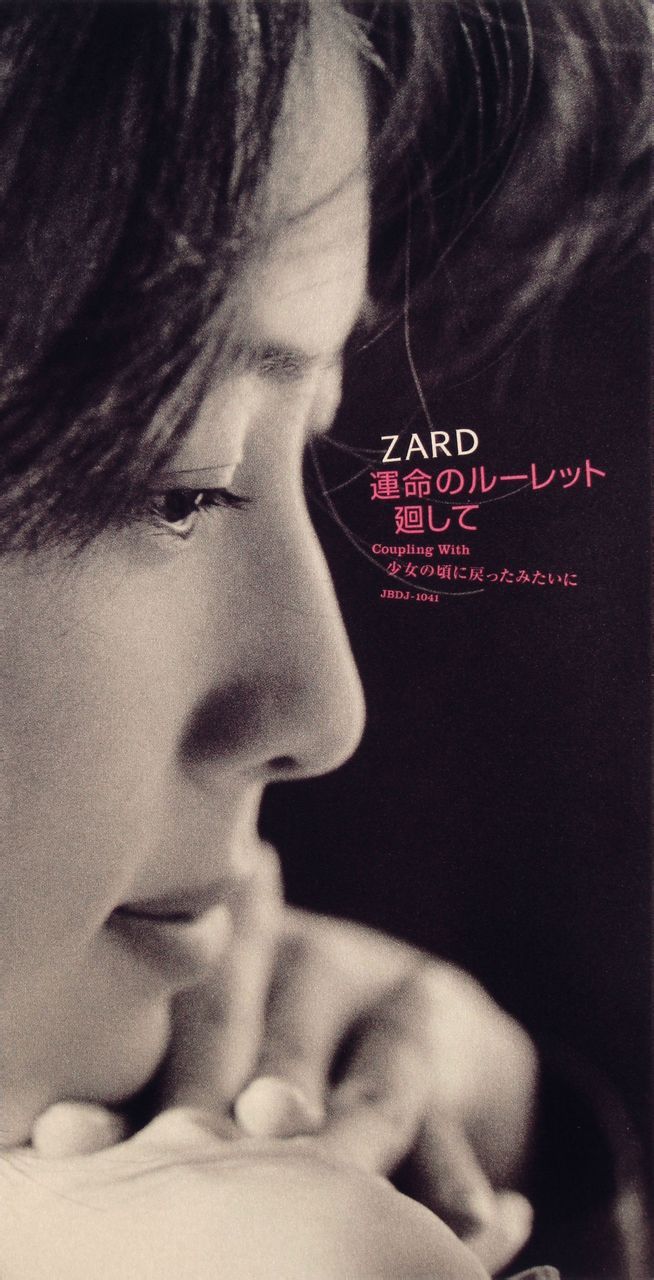
\includegraphics[width=0.3\textwidth]{S25.jpg}}

\large{

\ruby{運命}{うんめい}の\ruby{ルーレット}{roulette}\ruby{廻}{まわ}して
\\

ずっと \ruby{君}{きみ}を\ruby{見}{み}ていた

\ruby{何故}{なぜ}なの こんなに \ruby{幸}{しあわ}せなのに

\ruby{水平線}{すいへいせん}を\ruby{見}{み}ると \ruby{哀}{かな}しくなる

あの\ruby{頃}{ころ}の\ruby{自分}{じぶん}を\ruby{遠}{とお}くで \ruby{見}{み}ている そんな\ruby{感}{かん}じ
\\

\ruby{運命}{うんめい}の\ruby{ルーレット}{roulette}\ruby{廻}{まわ}して

アレコレ\ruby{深}{ふか}く\ruby{考}{かんが}えるのは Mystery

ほら \ruby{運命}{うんめい}の\ruby{人}{ひと}はそこにいる

ずっと \ruby{君}{きみ}を\ruby{見}{み}ていた
\\

\ruby{星空}{ほしそら}を\ruby{見上}{みあ}げて \ruby{笑顔}{ウインク}ひとつで

この\ruby{高}{たか}い\ruby{所}{ところ}からでも \ruby{飛}{と}べそうじゃん

\ruby{スピード}{speed}\ruby{上}{あ}げ \ruby{望遠鏡}{ぼうえんきょう}を \ruby{覗}{のぞ}いたら

\ruby{未来}{みらい}が\ruby{見}{み}えるよ
\\

\ruby{運命}{うんめい}の\ruby{ルーレット}{roulette}\ruby{廻}{まわ}して

\ruby{何処}{どこ}に\ruby{行}{ゆ}けば \ruby{想}{おも}い\ruby{出}{で}に\ruby{会}{あ}える?

\ruby{青}{あお}い\ruby{地球}{ちきゅう}の ちっぽけな\ruby{二人}{ふたり}は

\ruby{今}{いま}も \ruby{進化}{しんか}し\ruby{続}{つづ}ける
\\

\ruby{運命}{うんめい}の\ruby{ルーレット}{roulette}\ruby{廻}{まわ}して

\ruby{旅立}{たびだ}つ\ruby{時}{とき}の\ruby{翼}{つばさ}は bravely

ほら どんな\ruby{時}{とき}も \ruby{幸運}{こううん}は\ruby{待}{ま}ってる

ずっと \ruby{君}{きみ}を\ruby{見}{み}ていた
\\

ずっと \ruby{君}{きみ}を\ruby{見}{み}ていた

}

\hypertarget{8_5}{}
\section{ 遠い星を数えて}
\large{

\ruby{時々}{ときどき} あなたとは \ruby{合}{あ}わないのかなと

\ruby{感}{かん}じる\ruby{時}{とき}もあったけど

でもたわいもない\ruby{事}{こと}で\ruby{見}{み}つめあって \ruby{笑}{わら}えばすべて\ruby{忘}{わす}れていた

そんな\ruby{風}{ふう}にして\ruby{過}{す}ごしてきたけど

ある\ruby{時}{とき} \ruby{偶然}{ぐぜん}わかったの

\ruby{自分}{じぶん}を\ruby{出}{だ}していたつもりが

\ruby{肝心}{かんじん}な\ruby{事}{こと} Yes No を\ruby{避}{さ}け \ruby{逃}{にげ}げていた
\\

\ruby{未來}{あした}より\ruby{遠}{とお}い\ruby{星}{ほし}を\ruby{數}{かぞ}えて

\ruby{碧}{あお}い\ruby{夢達}{ゆめたち} \ruby{抱}{だ}きしめて

その\ruby{時}{とき}はいつか トキメキの\ruby{星}{ほし}になる

\ruby{勇氣}{ゆうき}を\ruby{持}{も}って \ruby{君}{きみ}に\ruby{飛}{と}びこみたい
\\

\ruby{自分}{じぶん}の\ruby{中}{なか}に いろんな\ruby{自分}{じぶん}がいて

「\ruby{優}{やさ}しいから \ruby{苦}{くる}しむのよ」と

\ruby{時}{とき}には\ruby{前向}{まえむ}きな\ruby{自分}{じぶん}が \ruby{弱氣}{よわき}な\ruby{自分}{じぶん}を\ruby{叱}{しか}ったりする
\\

\ruby{淚}{なみだ}より\ruby{遠}{とお}い\ruby{星}{ほし}を\ruby{數}{かぞ}えて

カッコいいことって カッコ\ruby{惡}{わる}いよ

\ruby{醒}{さ}めてるよりも \ruby{感情}{かんじょう}で\ruby{生}{い}きてる\ruby{人}{ひと}

\ruby{熱}{あつ}い\ruby{君}{きみ}を\ruby{見}{み}てると \ruby{嬉}{うれ}しくなる
\\

\ruby{遠}{とお}い\ruby{星}{ほし}を\ruby{數}{かぞ}えて

カッコいいことって カッコ\ruby{惡}{わる}いよ

\ruby{醒}{さ}めてるよりも \ruby{感情}{かんじょう}で\ruby{生}{い}きてる\ruby{人}{ひと}

\ruby{熱}{あつ}い\ruby{君}{きみ}を\ruby{見}{み}てると \ruby{嬉}{うれ}しくなる

}

\hypertarget{8_6}{}
\section{ 新しいドア~冬のひまわり~}

\parpic[r]{
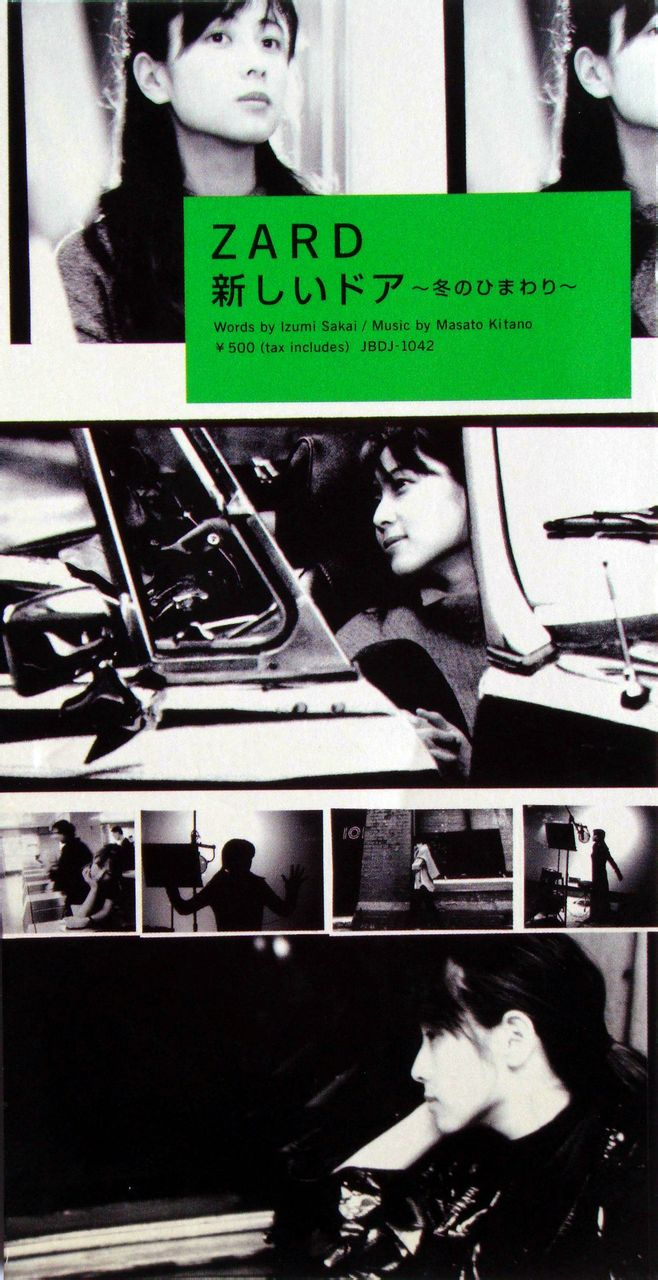
\includegraphics[width=0.3\textwidth]{S26.jpg}}

\large{

\ruby{通}{とお}り\ruby{雨}{あめ}の\ruby{中}{なか}で \ruby{抱}{だ}きしめた\ruby{君}{きみ}の\ruby{体温}{ぬくもり}

まだ この\ruby{胸}{むね}に \ruby{今}{いま}も \ruby{残}{のこ}っているよ
\\

\ruby{波}{なみ}に \ruby{揺}{ゆ}られながら

\ruby{泣}{な}いているだけの\ruby{夜}{よる}にサ·ヨ·ナ·ラ

\ruby{口笛}{くちぶえ}\ruby{吹}{ふ}いた あの\ruby{帰}{かえ}り\ruby{道}{みち}

ずっと \ruby{夕}{ゆ}\ruby{焼}{や}け \ruby{追}{お}いかけた
\\

はるかな\ruby{未来}{みらい}へと \ruby{新}{あたら}しい\ruby{ドア}{Door}を\ruby{開}{あ}け

\ruby{動}{うご}き\ruby{始}{はじ}めた \ruby{直感}{ちょっかん}が\ruby{行}{い}く\ruby{道}{みち}を\ruby{決}{き}める

あの\ruby{冬}{ふゆ}の\ruby{向日葵}{ひまわり}

まだひとりでやれそうだよ

\ruby{愛}{あい}する\ruby{人}{ひと}よ \ruby{今}{いま}どこで\ruby{眠}{ねむ}っていますか?

sweet pain \ruby{永遠}{えいえん}にとり\ruby{戻}{もど}せない あの\ruby{季節}{きせつ}
\\

\ruby{外}{そと}はこんなに \ruby{晴}{は}れているのに

\ruby{君}{きみ}の リンカクは ぼやけたまま

\ruby{無邪気}{むじゃき}に\ruby{笑}{わら}いあう あの\ruby{空}{そら}は\ruby{夢}{ゆめ}の\ruby{中}{なか}
\\

あの\ruby{時}{とき} \ruby{見}{み}えなかった\ruby{事}{こと}が

\ruby{今}{いま} \ruby{少}{すこ}しづつ わかりはじめているよ

スゴイケンカして \ruby{泣}{な}き\ruby{出}{だ}して\ruby{一人}{ひとり}

\ruby{先}{さき}に\ruby{帰}{かえ}った あの\ruby{渚}{なぎさ}
\\

\ruby{光}{ひか}る\ruby{夏}{なつ}に\ruby{生}{う}まれた \ruby{新}{あたら}しい\ruby{風}{かぜ}を\ruby{受}{う}け

まぶしい\ruby{空}{そら}を いくつも\ruby{超}{こ}えてゆきたい

\ruby{名前}{なまえ}なんか \ruby{知}{し}らなくても

\ruby{軽}{かる}い\ruby{ジョーク}{Joke}で\ruby{笑}{わら}えたね

あの\ruby{仲間達}{なかまたち} また\ruby{一緒}{いっしょ}に\ruby{行}{い}こうよ

I remember sweet memories

おかしいのに \ruby{何故}{なぜ}か\ruby{涙}{なみだ}が\ruby{出}{で}たよ
\\

はるかな\ruby{未来}{みらい}へと \ruby{新}{あたら}しい\ruby{ドア}{Door}を\ruby{開}{あ}け

\ruby{動}{うご}き\ruby{始}{はじ}めた \ruby{直感}{ちょっかん}が\ruby{行}{い}く\ruby{道}{みち}を\ruby{決}{き}める

あの\ruby{冬}{ふゆ}の\ruby{向日葵}{ひまわり}

まだひとりでやれそうだよ

\ruby{愛}{あい}する\ruby{人}{ひと}よ \ruby{今}{いま}どこで\ruby{眠}{ねむ}っていますか?

sweet pain \ruby{永遠}{えいえん}にとり\ruby{戻}{もど}せない あの\ruby{季節}{きせつ}
\\

sweet pain...
\\

\ruby{通}{とお}り\ruby{雨}{あめ}の\ruby{中}{なか}で \ruby{抱}{だ}きしめた\ruby{君}{きみ}の\ruby{体温}{ぬくもり}

まだこの\ruby{胸}{むね}に \ruby{今}{いま}も \ruby{残}{のこ}っているよ

}

\hypertarget{8_7}{}
\section{ Good day}

\parpic[r]{
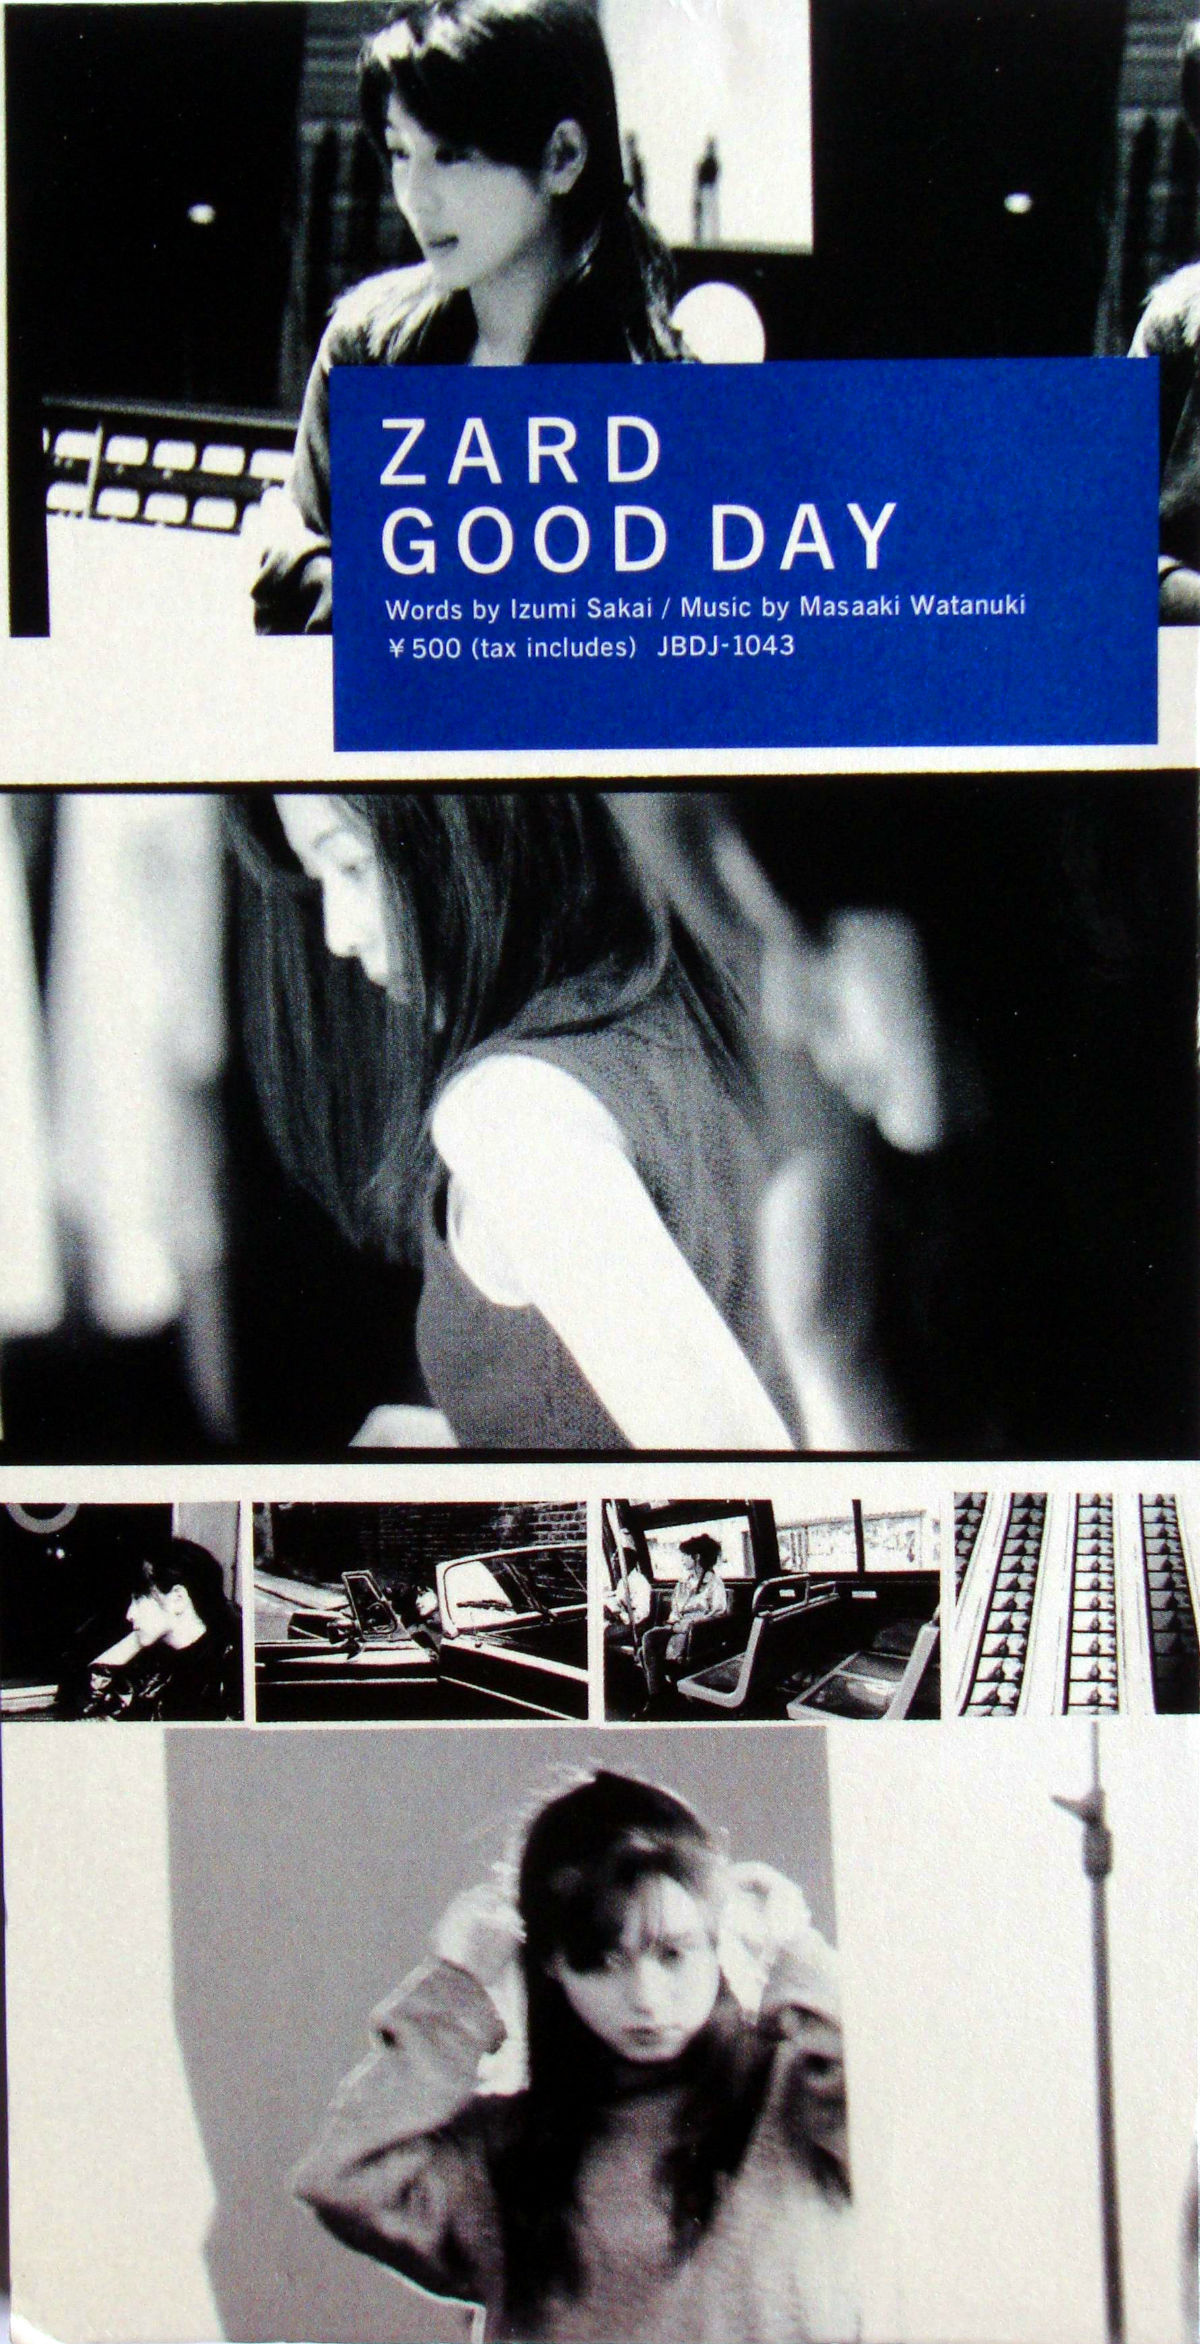
\includegraphics[width=0.3\textwidth]{S27.jpg}}

\large{

もし\ruby{翼}{つばさ}があったなら

\ruby{迷}{まよ}わずも forgive me kiss me

and hold me tight

あなたの\ruby{元}{もと}へと

\ruby{失}{うしな}った\ruby{歳月}{さいげつ}や \ruby{愛}{あい}を\ruby{連}{つら}れて

しがらみ\ruby{全部}{ぜんぶ} \ruby{脱}{ぬ}ぎ\ruby{捨}{す}てて
\\

Good day, and why don't you leave me alone

\ruby{諦}{あきら}めるよりも ああ \ruby{優}{やさ}しくなりたい

Good-bye, and somebody tell me why

\ruby{泣}{な}くから\ruby{悲}{かな}しくなるんだと
\\

\ruby{息}{いき}がつまりそうなこの\ruby{都会}{まち}

「\ruby{今日}{きょう} この\ruby{生活}{せいかつ}に \ruby{ピリオド}{period}\ruby{打}{う}つ\ruby{決心}{けっしん}をした」と

「\ruby{今度}{こんど}いつ\ruby{逢}{あ}えるの」と \ruby{聞}{き}けずに

\ruby{言葉}{ことば}はいつも \ruby{心}{こころ}とウラハラ
\\

Good day, and why don't you leave me alone

\ruby{諦}{あきら}めるよりも ああ \ruby{優}{やさ}しくなりたい

Good-bye, and somebody tell me why

\ruby{泣}{な}くから\ruby{悲}{かな}しくなるんだと
\\

もしあなたと このままいれば

きっと\ruby{後悔}{こうかい}する\ruby{日}{ひ}がくる
\\

Good day, and why don't you leave me alone

\ruby{諦}{あきら}めるよりも ああ \ruby{優}{やさ}しくなりたい

Good day \ruby{自分}{じぶん}の\ruby{弱}{よわ}さ \ruby{忘}{わす}れたいから

\ruby{人}{ひと}はまた\ruby{恋}{こい}に\ruby{落}{お}ちてゆく
\\

Good day, and why don't you leave me alone

\ruby{雨}{あめ}の\ruby{中}{なか}を どこまでも\ruby{歩}{ある}いた reason to cry

Good-bye, walk away, and don't you ask me why

サヨナラだけが \ruby{二人}{ふたり}に\ruby{残}{のこ}された\ruby{言葉}{ことば}…

}

\hypertarget{8_8}{}
\section{ I feel fine, yeah}
\large{

ほらほらそこの\ruby{君}{きみ} イライラしてる\ruby{君}{きみ}

\ruby{頭}{あたま}から\ruby{角}{つの}が\ruby{2本}{にほん} ニョキニョキ\ruby{生}{は}えてるよ

Look around the world \ruby{損}{そん}な\ruby{性格}{せいかく}!?

ココロだけが ナゼか\ruby{寒}{さむ}い \ruby{太陽}{たいよ}に\ruby{向}{む}かって\ruby{吠}{ほ}える!

\ruby{矛盾}{むじゅん}\ruby{矛盾}{むじゅん}の\ruby{日々}{ひび}  \ruby{友情}{ゆうじょう}の\ruby{絆}{きずな}にひび

\ruby{奇跡}{きせき}ねながっても \ruby{他力}{たりき}\ruby{本願}{ほんがん}でもいいんじゃない
\\

Look into the world \ruby{思}{おも}わず ゴツンッとぶつかって

ほんの\ruby{一秒}{いちびょう} \ruby{沈黙}{ちんもく}があったね

Don't look back こんな\ruby{風当}{かぜあ}たりの\ruby{強}{つよ}い\ruby{日}{ひ}は

\ruby{君}{きみ}と ここに うずくまっていたい

The sun in the sky やがて\ruby{朝}{あさ}が\ruby{来}{き}て

みえないチカラが… I feel fine, yeah
\\

\ruby{精}{せい}いっぱいの\ruby{愛}{あい}だから \ruby{自分}{じぶん}らしい\ruby{生}{い}きてゆこう

\ruby{心}{こころ}わけ\ruby{合}{あ}えばみんな ひとつになれるよ
\\

モクモク\ruby{仕事}{しごと}して \ruby{人}{ひと}の\ruby{2倍}{にばい}\ruby{仕事}{しごと}して

\ruby{頭}{あたま}から\ruby{角}{つの}が\ruby{2本}{にほん} ニョキニョキ\ruby{生}{は}えてるよ
\\

Look into the world \ruby{笑}{わら}うかどに むきかえる!

いつかは \ruby{偉}{えら}い\ruby{人}{ひと}になっているかも

Don't look back \ruby{気}{き}まぐれに\ruby{振}{ふ}り\ruby{回}{まわ}されても

いったい\ruby{今頃}{いまごろ} アナタ\ruby{誰}{だれ}といるの?

Sun rise in my heart やがて\ruby{日}{ひ}は\ruby{昇}{のぼ}ってく

\ruby{動}{うご}きだす\ruby{街}{まち}に I feel fine, yeah
\\

\ruby{情}{なさ}けないと\ruby{見}{み}せても \ruby{自分}{じぶん}らしく\ruby{生}{い}きてゆこう

\ruby{心}{こころ}\ruby{開}{ひら}けばみんな ひとつになれるよ

ひとつになれるよ

}

\hypertarget{8_9}{}
\section{ 少女の頃に戻ったみたいに}
\large{

くり\ruby{返}{かえ}し\ruby{見}{み}る\ruby{夢}{ゆめ}に

\ruby{目}{め}が\ruby{覚}{さ}めてみると

\ruby{胸}{むね}の\ruby{動悸}{どうき}が \ruby{早}{はや}いことに\ruby{気}{き}づく

いつも\ruby{白線}{はくせん} \ruby{踏}{ふ}みはずして

\ruby{走}{はし}る\ruby{私}{わたし}がいる

\ruby{何故}{なぜ}? \ruby{理由}{わけ}もないのに \ruby{声}{こえ}をあげて\ruby{泣}{な}きたくなる
\\

\ruby{幼}{おさな}い \ruby{少女}{しょうじょ}の\ruby{頃}{ころ}に\ruby{戻}{もど}ったみたいに

やさしく \ruby{髪}{かみ}を\ruby{撫}{な}でてくれる

そんな\ruby{温}{あたた}かい\ruby{手}{て}を いつも\ruby{待}{ま}っていた

あなただけは \ruby{私}{わたし}を やさしい\ruby{人}{ひと}にしてくれる

とても \ruby{大好}{だいす}きよ とても \ruby{大好}{だいす}きよ
\\

どんなに\ruby{情熱}{じょうねつ} かたむけても

わかりあえない \ruby{人}{ひと}もいる

そんな\ruby{日}{ひ}は \ruby{心}{こころ}が \ruby{曇}{くも}ってしまうわ

\ruby{恋}{こい}は\ruby{規則}{きそく}\ruby{正}{ただ}しい \ruby{リズム}{rhythm}を\ruby{刻}{きざ}まない

\ruby{心地}{ここち}\ruby{良}{い}い\ruby{ソファー}{sofa}で また \ruby{眠}{ねむ}ってしまった
\\

\ruby{懐}{なつ}かしい \ruby{少女}{しょうじょ}の\ruby{頃}{ころ}に\ruby{戻}{もど}ったみたいに

やさしく \ruby{髪}{かみ}を\ruby{撫}{な}でてくれる

そんな\ruby{温}{あたた}かい\ruby{手}{て}を いつも\ruby{待}{ま}っていた

あなただけは \ruby{私}{わたし}を そっと\ruby{包}{つつ}みこんでくれる

とても \ruby{愛}{あい}してる とても \ruby{愛}{あい}してる
\\

あなただけは \ruby{私}{わたし}を そっと\ruby{包}{つつ}みこんでくれる

とても \ruby{愛}{あい}してる \ruby{赤}{あか}い\ruby{ハート}{heart}で
\\

lovin' you あなたと…

}

\hypertarget{8_10}{}
\section{ 息もできない}

\parpic[r]{

\includegraphics[width=0.3\textwidth]{S24.jpg}}

\large{

\ruby{息}{いき}もできないくらい ねえ \ruby{君}{きみ}に\ruby{夢中}{むちゅう}だよ

\ruby{離}{はな}れてても \ruby{腕}{うで}の\ruby{中}{なか}にいる\ruby{気}{き}がするのは\ruby{何故}{なぜ}
\\

\ruby{耳}{みみ}をすませば \ruby{聞}{き}こえる\ruby{君}{きみ}の\ruby{鼓動}{こどう}

\ruby{世界中}{せかいじゅう}で\ruby{私}{わたし}だけが\ruby{聴}{き}いている\ruby{音}{おと}

\ruby{一人}{ひとり}でいる\ruby{時間}{とき}も

\ruby{友達}{ともだち}や\ruby{家族}{かぞく}とたわいなく\ruby{話}{はな}す\ruby{話題}{わだい}も

\ruby{大切}{たいせつ}な\ruby{時間}{じかん}だけど
\\

\ruby{息}{いき}もできないくらい ねえ \ruby{君}{きみ}が\ruby{好}{す}きだよ

ときどき\ruby{過去}{かこ}の\ruby{失恋}{きおく}に\ruby{臆病}{おくびょう}になるけど

\ruby{夕陽}{ゆうひ}に\ruby{横顔}{よこがお}の\ruby{シルエット}{Silhouette} 

ずっとそばにいたい

\ruby{限界}{げんかい}なんてまだ\ruby{遠}{とお}い 

この\ruby{恋}{こい}を\ruby{叶}{かな}えてください
\\

\ruby{恋}{こい}の\ruby{相談}{そうだん}をしているうちに

あの\ruby{時}{とき} \ruby{笑顔}{えがお}がすべてを \ruby{受}{う}け\ruby{入}{い}れてくれた

\ruby{疑}{うたが}う\ruby{心}{こころ} \ruby{迷}{まよ}う\ruby{気持}{きも}ち \ruby{口}{くち}に\ruby{出}{だ}せない

\ruby{君}{きみ}から\ruby{見}{み}た\ruby{私}{わたし}は どんな\ruby{風}{ふう}にみえるの
\\

どうでもいいこと\ruby{気}{き}にするところ \ruby{二人}{ふたり}よく\ruby{似}{に}ているね

\ruby{理解}{りかい}されなくても \ruby{絶対}{ぜったい} \ruby{妥協}{だきょう}しないでね

\ruby{想像力}{そうぞうりょく}の\ruby{中}{なか}で\ruby{世界}{せかい}は ぐんぐん ふくらんで\ruby{行}{い}く

\ruby{誰}{だれ}よりも \ruby{今}{いま}\ruby{近}{ちか}くに \ruby{君}{きみ}を\ruby{感}{かん}じているから
\\

\ruby{息}{いき}もできないくらい ねえ \ruby{君}{きみ}に\ruby{夢中}{むちゅう}だよ

\ruby{月}{つき}に\ruby{照}{て}らす \ruby{ジェットコースター}{Jet Coaster}が \ruby{闇}{やみ}をつき\ruby{抜}{ぬ}けていく

\ruby{明日}{あした}の\ruby{予定}{よてい}なんて \ruby{全部}{ぜんぶ}\ruby{キャンセル}{Cancel}してもいい

\ruby{今度}{こんど}こそは\ruby{本物}{ほんもの}だって \ruby{神様}{かみさま} \ruby{信}{しん}じていいですか
\\

\ruby{コート}{Coat}を\ruby{脱}{ぬ}ぐと\ruby{新}{あたら}しい\ruby{季節}{きせつ}が\ruby{動}{うご}き\ruby{出}{だ}す…

}

\hypertarget{8_11}{}
\section{ 風が通り抜ける街へ}

\large{

\ruby{思}{おも}いっきり \ruby{抱}{だ}きしめてね

\ruby{風}{かぜ}が\ruby{通}{とお}り\ruby{抜}{ぬ}ける\ruby{街}{まち}へ

\ruby{休}{やす}んでなんかいられない 

もう\ruby{乗}{の}りかかった\ruby{恋}{こい}だわ
\\

あなたの\ruby{手}{て}の\ruby{中}{なか}に 

すごい\ruby{引力}{いんりょく}で\ruby{落}{お}ちた

\ruby{好}{す}きでいると \ruby{嫌}{きら}われちゃうなら

このままの\ruby{関係}{かんけい}を\ruby{壊}{こわ}したくない

でもあなたのとなりで\ruby{平気}{へいき}な\ruby{顔}{かお}をしているのは もう\ruby{限界}{げんかい}
\\

\ruby{焼}{や}けた\ruby{肌}{はだ} \ruby{抱}{だ}きしめてね

\ruby{風}{かぜ}が\ruby{通}{とお}り\ruby{抜}{ぬ}ける\ruby{街}{まち}へ

\ruby{休}{やす}んでなんかいられない 

この\ruby{夏}{なつ}まで\ruby{待}{ま}てない
\\

このごろ\ruby{深刻}{しんこく}そうな\ruby{顔}{かお}ばかり… \ruby{話}{はな}して

\ruby{苦}{くる}しい\ruby{時}{とき} \ruby{孤独}{こどく}な\ruby{時}{とき}も

\ruby{見渡}{みわた}してみたら \ruby{見方}{みかた}がいるもの

\ruby{思}{おも}ったことを 

すぐ\ruby{口}{くち}に\ruby{出}{だ}してしまう 

\ruby{悪}{わる}いくせを\ruby{許}{ゆる}して
\\

\parpic[r]{
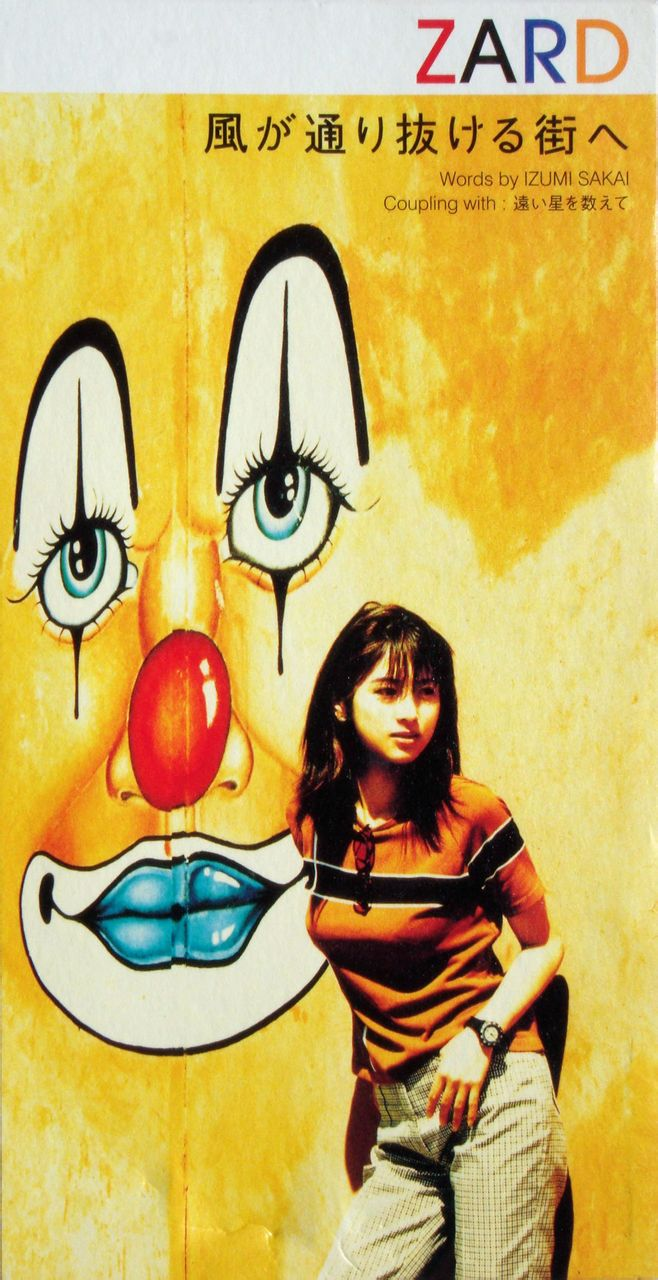
\includegraphics[width=0.3\textwidth]{S21.jpg}}

\ruby{思}{おも}いっきり \ruby{抱}{だ}きしめてね

\ruby{風}{かぜ}が\ruby{通}{とお}り\ruby{抜}{ぬ}ける\ruby{街}{まち}へ

\ruby{移}{うつ}り\ruby{気}{ぎ}な\ruby{季節}{きせつ}に 

もう\ruby{乗}{の}りかかった\ruby{恋}{こい}だわ
\\

あなたに\ruby{逢}{あ}えるから

\ruby{風}{かぜ}が\ruby{通}{とお}り\ruby{抜}{ぬ}ける\ruby{街}{まち}へ

\ruby{休}{やす}んでなんかいられない 

もう\ruby{乗}{の}りかかった\ruby{恋}{こい}だわ

この\ruby{夏}{なつ}まで\ruby{待}{ま}てない
\\

Just one look and I knew. Only one.

もう\ruby{乗}{の}りかかった\ruby{恋}{こい}だわ

}

\hypertarget{8_12}{}
\section{ フォトグラフ}
\large{

そこには まだ\ruby{虹}{にじ}があるの?

\ruby{花}{はな}たちが\ruby{育}{そだ}ってゆくの?

We laughed them all

\ruby{気}{き}づかない\ruby{程}{ほど}\ruby{若}{わか}くないし

\ruby{理解}{りかい}できない\ruby{程}{ほど}

\ruby{純真}{じゅんしん}でもない\ruby{天使}{てんし}たち

\ruby{本当}{ほんとう}は\ruby{怖}{こわ}くて \ruby{本当}{ほんとう}は\ruby{弱虫}{よわむし}

\ruby{帰}{かえ}る\ruby{家}{いえ}を\ruby{探}{さが}してる
\\

そばに\ruby{居}{い}るだけで それだけでよかった

\ruby{フォトグラフ}{photograph} \ruby{明日}{あした}が\ruby{見}{み}えなくても

ほら \ruby{君}{きみ}が\ruby{揺}{ゆ}れてる
\\

\ruby{窓辺}{まどべ}に\ruby{並}{なら}べかけた\ruby{植物}{はな}の\ruby{傍}{そば}に

ひとり\ruby{腰}{こし}かけた

There's no time at all

\ruby{思}{おも}い\ruby{入}{い}れが\ruby{強}{つよ}すぎると

\ruby{次}{つぎ}に\ruby{起}{お}こることが\ruby{噓}{うそ}のよう

もう\ruby{何年}{なんねん}ぐらい\ruby{過}{た}ったのだろう

すべてが\ruby{現実}{げんじつ} すべてがまぼろし

\ruby{帰}{かえ}る\ruby{道}{みち}を\ruby{探}{さが}してる
\\

\ruby{言葉}{ことば}はいらなかった

「\ruby{愛}{あい}してる」の\ruby{サイン}{sign}だけで

\ruby{フォトグラフ}{photograph} \ruby{砂}{すな}に\ruby{足跡}{あしあと}つけて

ほら \ruby{君}{きみ}が\ruby{笑}{わら}ってる
\\

そばに\ruby{居}{い}るだけで それだけでよかった

\ruby{瞳}{ひとみ}を\ruby{輝}{かがや}かせ \ruby{夢中}{むちゅう}になるクセ

\ruby{今}{いま}も \ruby{変}{か}わらずにいて

ほら \ruby{君}{きみ}が\ruby{愛}{いと}しい

}

{ \ }

{ \ }

{ \ }

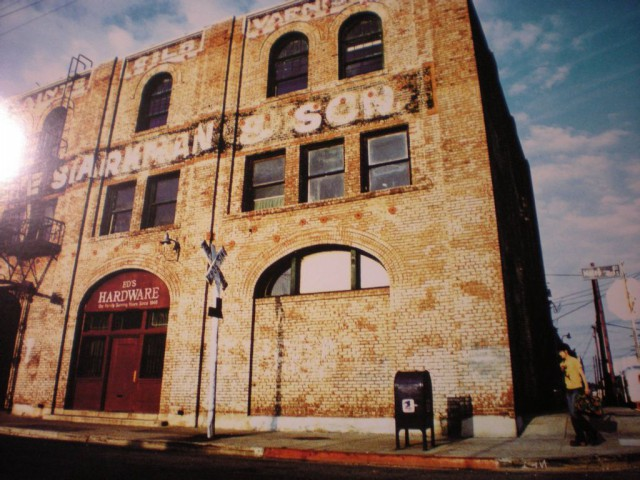
\includegraphics[width=0.9\textwidth]{P6.jpg}


\chapter{Album 9}
\thispagestyle{empty} %本页頁碼空白
\vspace{-16mm}
\LARGE {時間(とき)の翼}

\normalsize{JBCJ-1033 2001.2.15 \ release}
\\

\vspace{-5mm}

\parpic[l]{
\pichskip{6em}
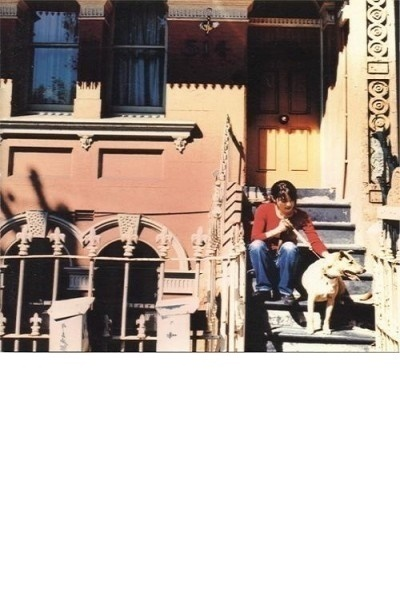
\includegraphics[width=0.4\textwidth]{9.jpg}}

\small{\hyperlink{9_0}{1.Get U're Dream}}

\tiny{作詞:坂井泉水 \ 作曲:大野愛果 \ 編曲:葉山たけし}

\small{\hyperlink{9_1}{2.この涙 星になれ}}

\tiny{作詞:坂井泉水 \ 作曲:岩井勇一郎 \ 編曲:古井弘人}

\small{\hyperlink{9_2}{3.promised you ~with P-edition~}}

\tiny{作詞:坂井泉水 \ 作曲:栗林誠一郎 \ 編曲:Cybersound}

\small{\hyperlink{9_3}{4.痛いくらい君があふれているよ}}

\tiny{作詞:坂井泉水 \ 作曲/編曲:シオジリケンジ}

\small{\hyperlink{9_4}{5.窓の外はモノクローム}}

\tiny{作詞:坂井泉水 \ 作曲:岩井勇一郎 \ 編曲:大賀好修}

\small{\hyperlink{9_5}{6.お・も・ひ・で}}

\tiny{作詞:坂井泉水 \ 作曲:寺尾広 \ 編曲:古井弘人}

\small{\hyperlink{9_6}{7.明日もし君が壊れても}}

\tiny{作詞:坂井泉水 \ 作曲:大野愛果 \ 編曲:徳永暁人}

\small{\hyperlink{9_7}{8.世界はきっと未来の中}}

\tiny{作詞:坂井泉水 \ 作曲:岩井勇一郎 \ 編曲:徳永暁人/古井弘人/シオジリケンジ}

\small{\hyperlink{9_8}{9.hero}}

\tiny{作詞:坂井泉水 \ 作曲:大野愛果 \ 編曲:大賀好修}
\begin{comment}
\small{\hyperlink{9_9}{10.揺れる想い Gomi's New York Remix}}

\small{\hyperlink{9_10}{11.負けないで Gomi's 10th Anni. Special Mix}}
\end{comment}

\small{\hyperlink{9_9}{10.時間の翼}}

\tiny{作詞:坂井泉水 \ 作曲:大野愛果 \ 編曲:徳永暁人}

\clearpage


\hypertarget{9_0}{}
\section{ Get U're Dream}
\large{

\ruby{君}{きみ}の\ruby{瞳}{ひとみ}に\ruby{星}{ほし}が\ruby{輝}{かがや}き \ruby{醒}{さ}めた\ruby{心}{こころ}とかしてゆく

\ruby{夢}{ゆめ}のために \ruby{愛}{あい}のために you're so far away
\\

\parpic[r]{

\includegraphics[width=0.4\textwidth]{S32.jpg}}

あんなに\ruby{燃}{も}えた \ruby{夏}{なつ}が\ruby{過}{す}ぎると

せつない\ruby{夜}{よる}が\ruby{長}{なが}くなる

もしも \ruby{別}{わか}れるようなことになっても

\ruby{変}{か}わらず \ruby{友達}{ともだち}でいようね

いつまでも \ruby{永遠}{とわ}のDestiny

\ruby{信}{しん}じてたね \ruby{無}{む}\ruby{邪気}{じゃき}な\ruby{日々}{ひび}
\\

たとえ\ruby{遠}{とお}く \ruby{離}{はな}れてても

I hear your voice \ruby{君}{きみ}の\ruby{声}{こえ}が

\ruby{倒}{たお}れそうになった\ruby{時}{とき} かすかに\ruby{声}{こえ}が\ruby{聞}{き}こえた

I wanna be with you, but you're far away

だけど\ruby{夢}{ゆめ}や\ruby{希望}{きぼう}があるから

\ruby{今}{いま}よりもっと\ruby{強}{つよ}くなれるはず

I will…, Get U're Dream !
\\

\ruby{走}{はし}り\ruby{疲}{つか}れて \ruby{瞳}{ひとみ}\ruby{閉}{と}じると

\ruby{君}{きみ}の\ruby{香}{かお}り \ruby{鼓動}{こどう}を\ruby{熱}{あつ}くする

\ruby{夜明}{よあ}けの Sweet Destiny

\ruby{今}{いま}も \ruby{深}{ふか}まってゆく \ruby{君}{きみ}への\ruby{愛情}{あいじょう}
\\

\ruby{寂}{さび}しい\ruby{夜}{よる} いくつ\ruby{君}{きみ}と \ruby{越}{こ}えただろう

\ruby{見知}{みし}らぬ\ruby{街}{まち}

\ruby{夜}{よる}\ruby{遅}{おそ}くまで\ruby{話}{はな}し\ruby{込}{こ}んでは \ruby{送}{おく}ってくれたね

I wanna be with you, but you're far away

\ruby{孤独}{こどく}だけど きっと\ruby{叶}{かな}えるよ

\ruby{少}{すこ}しでも \ruby{伝}{つた}えたくて

\ruby{君}{きみ}に\ruby{届}{とど}け let's make your dream!
\\

Nobody else in sight

And I am feelin' good just holding you tight

I close my eyes
\\

You make me smile

I will be dreaming of you
\\

たとえ\ruby{遠}{とお}く \ruby{離}{はな}れてても

I hear your voice \ruby{君}{きみ}の\ruby{声}{こえ}が

\ruby{倒}{たお}れそうになった\ruby{時}{とき} \ruby{確}{たし}かに\ruby{声}{こえ}が\ruby{聞}{き}こえた
\\

\ruby{明日}{あした}のこと \ruby{判}{わか}らなくても

\ruby{君}{きみ}といると \ruby{笑}{わら}っていたよね

you make me smile \ruby{忘}{わす}れないで

\ruby{君}{きみ}に\ruby{届}{とど}け きっと… Get U're Dream !
\\

you make me smile \ruby{変}{か}わらないで

\ruby{君}{きみ}に\ruby{届}{とど}け きっと… Get U're Dream !

}

\hypertarget{9_1}{}
\section{ この涙 星になれ}

\parpic[r]{
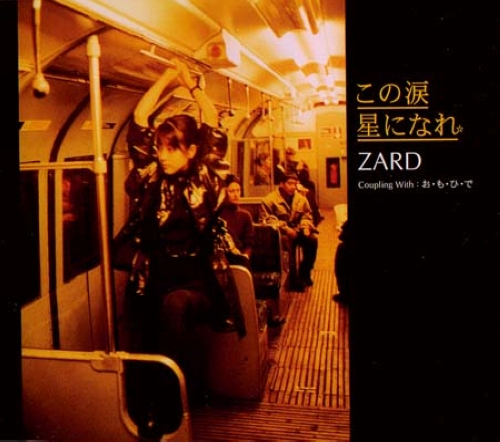
\includegraphics[width=0.4\textwidth]{S31.jpg}}

\large{

\ruby{窓}{まど}の\ruby{外}{そと}が

\ruby{白}{しろ}くなる\ruby{瞬間}{しゅんかん}が\ruby{好}{す}き

\ruby{絶望}{ぜつぼう}と\ruby{希望}{きぼう}の\ruby{狭間}{はざま}で
\\

\ruby{失敗}{しっぱい}は\ruby{誰}{だれ}かのせいに

したくなるけど

それを\ruby{乗}{の}り\ruby{越}{こ}えよう
\\

そう\ruby{人生}{じんせい}はいつだってオーディション

\ruby{動}{うご}き\ruby{出}{だ}してる signal

その\ruby{一瞬}{いっしゅん}は\ruby{戻}{もど}らない
\\

\ruby{愛}{あい}し\ruby{始}{はじ}めてた…

\ruby{少}{すこ}しの\ruby{笑顔}{えがお}でよかったのに

いつからか\ruby{気軽}{きがる}に

\ruby{君}{きも}と\ruby{話}{はな}せなくなってた
\\

I'm so in love with you

\ruby{都会}{とかい}の\ruby{雨}{あめ}は\ruby{冷}{さめ}たいね ah

fakeの\ruby{中}{なか}で

この\ruby{涙}{なみだ} \ruby{星}{ほし}になれ
\\

\ruby{誰}{だれ}かに\ruby{相談}{そうだん}したら

\ruby{迷}{まよ}っちゃいそうだったから

ゴメンネ \ruby{黙}{だま}ってここを\ruby{出}{で}ていく
\\

\ruby{父}{ちち}なる\ruby{砂漠}{さばく} コイン\ruby{投}{な}げて

\ruby{明日}{あした}を\ruby{占}{うらん}おう
\\

そう\ruby{人生}{じんせい}はままならぬ No Reaction

\ruby{案外}{あんがい} \ruby{君}{きみ}の\ruby{素顔}{すがた}は

\ruby{涙}{なみだ}もろいって\ruby{知}{し}ってる
\\

coolな\ruby{都会}{とかい}の\ruby{中}{なか}

\ruby{本当}{ほんとう}の\ruby{愛}{あい}\ruby{見}{み}つけよう

\ruby{暗闇}{くらやみ}で\ruby{原石}{げんせき}は\ruby{輝}{かがや}いているよ
\\

And Nothing to get hung about

\ruby{君}{きみ}の\ruby{記憶}{きおく}が\ruby{全部}{ぜんぶ}\ruby{消}{き}えてしまう\ruby{前}{まえ}に

I'll be back

この\ruby{涙}{なみだ} \ruby{星}{ほし}になれ
\\

そして\ruby{時間}{とき}が\ruby{過}{す}ぎ…\ruby{希望}{きぼう}が\ruby{人}{ひと}を\ruby{支}{ささ}えるから

こんなに\ruby{寒}{さむ}い\ruby{夜}{よる}は \ruby{成長}{せいちょう}してゆくんだね…
\\

And Nothing to get hung about

\ruby{君}{きみ}の\ruby{記憶}{きおく}が\ruby{全部}{ぜんぶ}\ruby{消}{き}えてしまう\ruby{前}{まえ}に

I'll be back

この\ruby{涙}{なみだ} \ruby{星}{ほし}になれ

}

\hypertarget{9_2}{}
\section{ promised you~with P-edition~}

\parpic[r]{
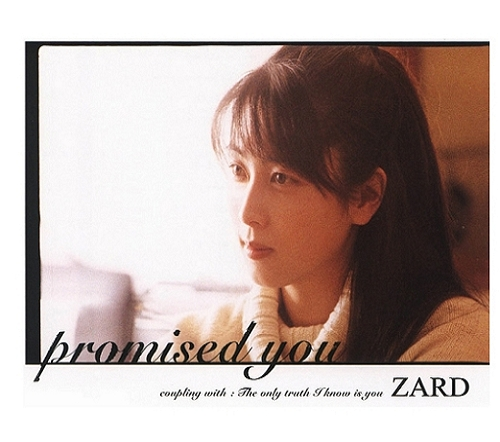
\includegraphics[width=0.4\textwidth]{S33.jpg}}

\large{

\ruby{土曜}{どよう}には\ruby{珍}{めずら}しく \ruby{人通}{ひとどお}りが\ruby{少}{すく}ない

いつからか \ruby{不安}{ふあん}な\ruby{雨}{あめ}が\ruby{降}{ふ}る

あの\ruby{頃}{ころ}の\ruby{思}{おも}い\ruby{出}{で}が\ruby{懷}{なつ}かしい

\ruby{君}{きみ}は\ruby{深}{ふか}く \ruby{眠}{ねむ}っていたよね
\\

\ruby{戀}{こい}がいつか\ruby{愛}{あい}に\ruby{變}{か}わった

promised you また\ruby{始}{はじ}めよう

\ruby{白}{しろ}く\ruby{煙}{けむ}った\ruby{宇宙}{うちゅう}に 

みんな\ruby{笑}{わら}って生きてる
\\

\ruby{長}{なが}い\ruby{冬}{ふゆ}が\ruby{終}{おわ}わって promised you また\ruby{始}{はじ}めよう

\ruby{白}{しろ}く\ruby{煙}{けむ}った\ruby{宇宙}{うちゅう}に みんな\ruby{笑}{わら}って生きてる
\\

どうして\ruby{君}{きみ}のそばにいると

こんなに\ruby{口下手}{くちべた}になっちゃうんだろう

なんでそんなに\ruby{速}{はや}く\ruby{步}{ある}くのかな

スピード\ruby{落}{お}としたら \ruby{樂}{らく}なのに
\\

どこに\ruby{行}{い}くのかも\ruby{判}{わか}らず あの\ruby{時}{とき}

promised you サヨナラしたけど

\ruby{誰}{だれ}も\ruby{知}{し}らない \ruby{二人}{ふたり}が\ruby{孤獨}{こどく}だったことなんて
\\

\ruby{離}{はな}れて\ruby{初}{はじ}めて\ruby{氣付}{きつ}いた promised you そう\ruby{時}{とき}は\ruby{過}{す}ぎ

\ruby{私}{わたし}は\ruby{何}{なに}かを\ruby{守}{まも}っていた\ruby{氣}{き}になっていただけ
\\

Remember I'll always be true

promised you so special one for me

\ruby{心}{こころ}の\ruby{中}{なか}で\ruby{動}{うご}き\ruby{出}{だ}す \ruby{淡}{あわ}い\ruby{君}{きみ}との\ruby{時間}{じかn}
\\

\ruby{戀}{こい}がいつか\ruby{愛}{あい}に\ruby{變}{か}わった

promised you また\ruby{始}{はじ}めよう

\ruby{白}{しろ}く\ruby{煙}{けむ}った\ruby{宇宙}{うちゅう}に みんな\ruby{笑}{わら}って生きてる

}

\hypertarget{9_3}{}
\section{ 痛いくらい君があふれているよ}

\parpic[r]{
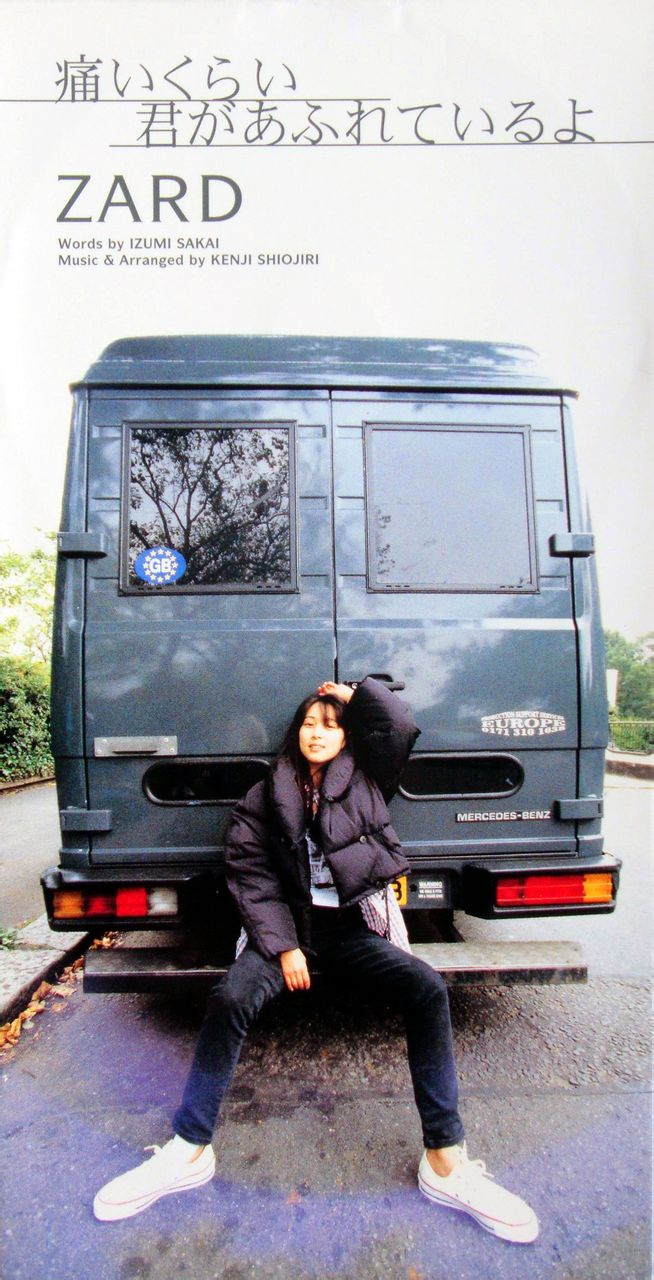
\includegraphics[width=0.3\textwidth]{S30.jpg}}

\large{

あなたの\ruby{夢}{ゆめ}が いつか\ruby{叶}{かない}いますように

\ruby{暮}{く}れることのない この\ruby{國}{くに}に
\\

\ruby{一日}{いちにち}\ruby{逢}{あ}えないだけで\ruby{逢}{あ}えばドキ

ドキッ キスするだけで\ruby{胸}{むね}もドキ

ドキッ \ruby{計算}{けいさん}しだしたらもう\ruby{逃}{に}げる\ruby{時}{とき}

そう\ruby{居心地}{いごこち}のいい\ruby{腕}{うで}
\\

\ruby{澀滯}{じゅうたい}の\ruby{中}{なか}から\ruby{拔}{ぬ}けだそう

\ruby{互}{たが}いに\ruby{言}{い}わなくなったね「ありがとう」

もう\ruby{誕生日}{たんじょうび}を\ruby{祝}{いわ}ってもらう

%\ruby{歲}{とし}

(とし)じゃないし でも

Kiss me brother (right now)
\\

\ruby{朝}{あさ}が來るまで \ruby{情熱}{じょうねつ}や

「\ruby{痛}{いた}み」を\ruby{感}{かん}じていたいのずっと

\ruby{戀}{こい}してるチカラ カタチ

ほっぺをくっつけて\ruby{眠}{ねむ}りたい
\\

\ruby{痛}{いた}いくらい\ruby{君}{きみ}があふれているよ

Just moment \ruby{今}{いま}  \ruby{時間}{じかん}が\ruby{動}{うご}き\ruby{出}{で}してる

せつなくて せつなくて \ruby{君}{きみ}に\ruby{逢}{あ}いたいよ

Love & Peace

\ruby{都會}{とかい}はいつも \ruby{誰}{だれ}かの目が\ruby{光}{ひが}ってる

Just can't buy me love

Just can't buy me love
\\

どんなに\ruby{便利}{べんり}になっても

ちゃんと\ruby{君}{きみ}と\ruby{顏}{かお}\ruby{見}{み}て\ruby{話}{はな}したい

\ruby{屁理屈大王}{へりくつだいおう} こんな

ケンカ \ruby{今日}{きょう}で \ruby{終}{お}りにしたい

あの\ruby{頃}{ころ}は\ruby{母}{はは}の\ruby{愛情}{あいじょう}さえも

\ruby{重}{おも}かった それぞれの\ruby{事情}{じじょう}

with all heart feel all my soul

\ruby{贅澤}{ぜいたく}は\ruby{夢}{ゆめ}を\ruby{食}{た}べてしまうから!
\\

\ruby{痛}{いた}いくらい\ruby{君}{きみ}があふれているよ

Just moment \ruby{今}{いま} \ruby{時間}{じかん}が\ruby{動}{うご}き\ruby{出}{だ}してる

せつなくて せつなくて \ruby{君}{きみ}に\ruby{逢}{あ}いたいよ

Love & Peace \ruby{流}{なが}れ\ruby{星}{ぼし}

\ruby{同}{おなじ}じ\ruby{每日}{まいにち}なんて \ruby{煮}{に}つまる!

\ruby{君}{きみ}のロケットで \ruby{強}{つよ}く\ruby{擊}{う}ち\ruby{拔}{ぬ}いて

\ruby{誰}{だれ}かが\ruby{鄰}{となり}の\ruby{部屋}{へや}で \ruby{騷}{さわ}いでる (Your mind aches)

\ruby{月曜}{げつよう}の\ruby{朝}{あさ}が\ruby{來}{く}る (Your day breaks) escape!
\\

a ah ah

I need to laugh

And well,well…when the sun is out
\\

\ruby{痛}{いた}いくらい\ruby{君}{きみ}があふれているよ

Just moment \ruby{今}{いま} \ruby{時間}{じかん}が\ruby{動}{うご}き\ruby{出}{だ}してる

ずっと\ruby{見守}{みまも}ってくれるというけれど

when will be love long time

いつまで\ruby{待}{ま}てばいい?このモヤモヤは

パズルを\ruby{完成}{かんせい}させる \ruby{最後}{さいご}のピース

wow wow wow wow
\\

\ruby{君}{きみ}があふれている どんなときも

\ruby{笑}{わら}っていたいよね

}

\hypertarget{9_4}{}
\section{ 窓の外はモノクローム}
\large{

\ruby{歩}{ある}き\ruby{出}{だ}すその\ruby{道}{みち}は

どこかに\ruby{繫}{つな}がってるの?

いくつもの \ruby{扉}{とびら}を\ruby{叩}{たた}いてきた

\ruby{移}{うつ}りゆく \ruby{人間}{ひと}\ruby{模様}{もよう}

\ruby{周囲}{まわり}が\ruby{羨}{うらや}むほど

\ruby{仲}{なか}が\ruby{良}{い}い\ruby{二人}{ふたり}だったのにね

まるで\ruby{鉄棒}{てつぼう}にぶらさがってるみたいに

\ruby{世界}{せかい}が\ruby{廻}{まわ}るのを \ruby{拒}{こば}んでいたい
\\

ドキドキした あの\ruby{懷}{なつ}かしい\ruby{ストーリー}{story}

となりにいる あなたも\ruby{夢中}{むちゅう}だった

\ruby{途切}{とぎ}れる\ruby{言葉}{ことば} いくつも \ruby{埋}{う}めるように

はしゃいだ\ruby{夜更}{よふ}けの\ruby{部屋}{へや}

\ruby{窓}{まど}の\ruby{外}{そと}は\ruby{モノクローム}{monochrome}
\\

ねぇ \ruby{例}{たと}えば

\ruby{道端}{みちばた}にさく \ruby{草花}{はな}を\ruby{見}{み}て

「\ruby{嫌}{きら}いだ」と

\ruby{思}{おも}えるうちは まだ\ruby{大丈夫}{だいじょうぶ}

もし\ruby{雨}{あめ}に\ruby{濡}{ぬ}れたなら

やさしく\ruby{傘}{かさ}をさしてくれたよね そこが\ruby{好}{す}きだったの

\ruby{噓}{うそ}をつくなら… そう\ruby{最後}{さいご}まで ずっと

ずっと \ruby{噓}{うそ}をつき\ruby{通}{とお}してほしかった
\\

ときどきあって\ruby{話}{はな}すことが\ruby{無}{な}くなって

こうして\ruby{別}{べつ}の\ruby{人生}{じんせい} \ruby{探}{さが}してる\ruby{方}{ほう}が…

\ruby{幸}{しあわ}せだね \ruby{輝}{かがや}ける\ruby{未来}{みらい}のために

\ruby{私}{わたし}は\ruby{泣}{な}かなかった

\ruby{窓}{まど}の\ruby{外}{そと}は\ruby{モノクローム}{monochrome}
\\

ドキドキした あの\ruby{懷}{なつ}かしい\ruby{ストーリー}{story}

となりにいる あなたも\ruby{夢中}{むちゅう}だった

\ruby{途切}{とぎ}れる\ruby{言葉}{ことば} いくつも \ruby{埋}{う}めるように

はしゃいだ\ruby{夜更}{よふ}けの\ruby{部屋}{へや}

\ruby{窓}{まど}の\ruby{外}{そと}は\ruby{モノクローム}{monochrome}

}

\hypertarget{9_5}{}
\section{ お·も·ひ·で}
\large{

まばたきをした\ruby{一瞬}{いっしゅん}に\ruby{思}{おも}い\ruby{出}{だ}す

あの\ruby{都会}{まち}

\ruby{遠}{とお}ざかる\ruby{大室山}{おおむろやま}の\ruby{夕暮}{ゆうぐ}れ

\ruby{愛}{いと}しき\ruby{日々}{ひび}

\ruby{切}{せつ}ない\ruby{想}{おも}い Just fallin'love

\ruby{夏}{なつ}の\ruby{終}{お}わりに
\\

\ruby{十年後}{じゅうねんご}の\ruby{アルバム}{album}を

いつか\ruby{開}{ひら}くように

\ruby{羽根}{はね}\ruby{休}{やす}めた \ruby{鳥}{とり}のように

この\ruby{静}{しず}けさの\ruby{中}{なか}で

everyday and night

\ruby{今}{いま}も \ruby{自分}{じぶん}の\ruby{夢}{ゆめ}を

\ruby{信}{しん}じていたいんです
\\

\ruby{晴}{は}れ\ruby{渡}{わた}る \ruby{穏}{おだ}やかな\ruby{波}{なみ}の

\ruby{調}{しら}べの\ruby{白浜}{しらはま}

\ruby{見失}{みうしな}う

\ruby{昔}{むかし}の\ruby{自分}{じぶん}を\ruby{取}{と}りもどしたくて

\ruby{待}{ま}ちあわせの\ruby{場所}{ばしょ} \ruby{間違}{まちが}えて

\ruby{映画}{えいが} \ruby{観}{み}れなくなったね
\\

\ruby{太陽}{たいよう}が\ruby{昇}{のぼ}るように

\ruby{前向}{まえむ}きに\ruby{生}{い}きたい

\ruby{自分}{じぶん}らしく\ruby{生}{い}きること

\ruby{自分}{じぶん}を\ruby{愛}{あい}すること

everyday and night

\ruby{君}{きみ}が\ruby{教}{おし}えてくれた

\ruby{遥}{はる}かな\ruby{希望}{きぼう}へと
\\

その\ruby{笑顔}{えがお} \ruby{忘}{わす}れないで

\ruby{経験}{けいけん} \ruby{重}{かさ}ねても

\ruby{失}{うしな}いたくない

\ruby{夢}{ゆめ}の\ruby{色}{いろ}が\ruby{塗}{ぬ}り\ruby{変}{か}わっても

everyday and night

\ruby{明日}{あす}の\ruby{風}{かぜ}に\ruby{向}{む}かって

\ruby{歩}{ある}き\ruby{出}{だ}そう \ruby{君}{きみ}と

}

\hypertarget{9_6}{}
\section{ 明日もし君が壊れても}
\large{

Call my name

\ruby{誰}{だれ}かが\ruby{呼}{よ}ぷ\ruby{声}{こえ}

\ruby{暗闇}{くらやみ}の\ruby{深}{ふか}い\ruby{悲}{かな}しみ

\ruby{白}{しろ}い\ruby{素肌}{すはだ}の\ruby{君}{きみ}が

\ruby{僕}{ぼく}のそこに\ruby{光}{ひかり}をさす

\ruby{黒}{くろ}か\ruby{白}{しろ}か\ruby{分}{わ}からないまま

こんな\ruby{愛}{あい}は\ruby{時代}{じだい}\ruby{遲}{おく}れるのか?

\ruby{僕}{ぼく}らは\ruby{一日中}{いちにちじゅう}

\ruby{朝}{あさ}が\ruby{訪}{おとず}れるのを\ruby{待}{ま}つだけ
\\

\ruby{明日}{あした}もし\ruby{君}{きみ}が\ruby{壞}{こわ}れても

ここから\ruby{逃}{に}げ\ruby{出}{だ}さない

\ruby{疲}{つか}れた\ruby{体}{からだ}を\ruby{癒}{いや}す

\ruby{君}{きみ}の\ruby{微笑}{ほほえ}みよ
\\

Lomely heart もて\ruby{余}{あま}す\ruby{心}{こころ}

ポッカリ\ruby{穴}{あな}が\ruby{空}{あ}いたようだ

\ruby{自分}{じぶん}を\ruby{抑}{おさ}えきれず\ruby{何}{なに}かに

イライラしてた

「あの\ruby{恋}{こい}を\ruby{忘}{わす}れられない」と

\ruby{出逢}{であ}ったころ\ruby{話}{はな}してたね

\ruby{本心}{ほんしん}を\ruby{隠}{かく}した\ruby{表情}{かお}

まだ\ruby{僕}{ぼく}には\ruby{救}{すく}いがありそう?
\\

\ruby{明日}{あした}もし\ruby{君}{きみ}が\ruby{壞}{こわ}れても

さまよい\ruby{続}{つづ}けるだろう

\ruby{愛}{あい}して\ruby{初}{はじ}めて\ruby{知}{し}った

\ruby{失}{うしな}う\ruby{怖}{こわ}さを
\\

\ruby{明日}{あした}もし\ruby{君}{きみ}が\ruby{壞}{こわ}れても

\ruby{何}{なに}も\ruby{見}{み}えなくなっても

\ruby{安}{やす}らかな\ruby{時}{とき}の\ruby{中}{なか}で

\ruby{僕}{ぼく}らは\ruby{歩}{ある}き\ruby{出}{だ}す

\ruby{君}{きみ}のまぼろしよ
\\

Call my name

Who are you?

Call my name

}

\hypertarget{9_7}{}
\section{ 世界はきっと未来の中}

\parpic[r]{
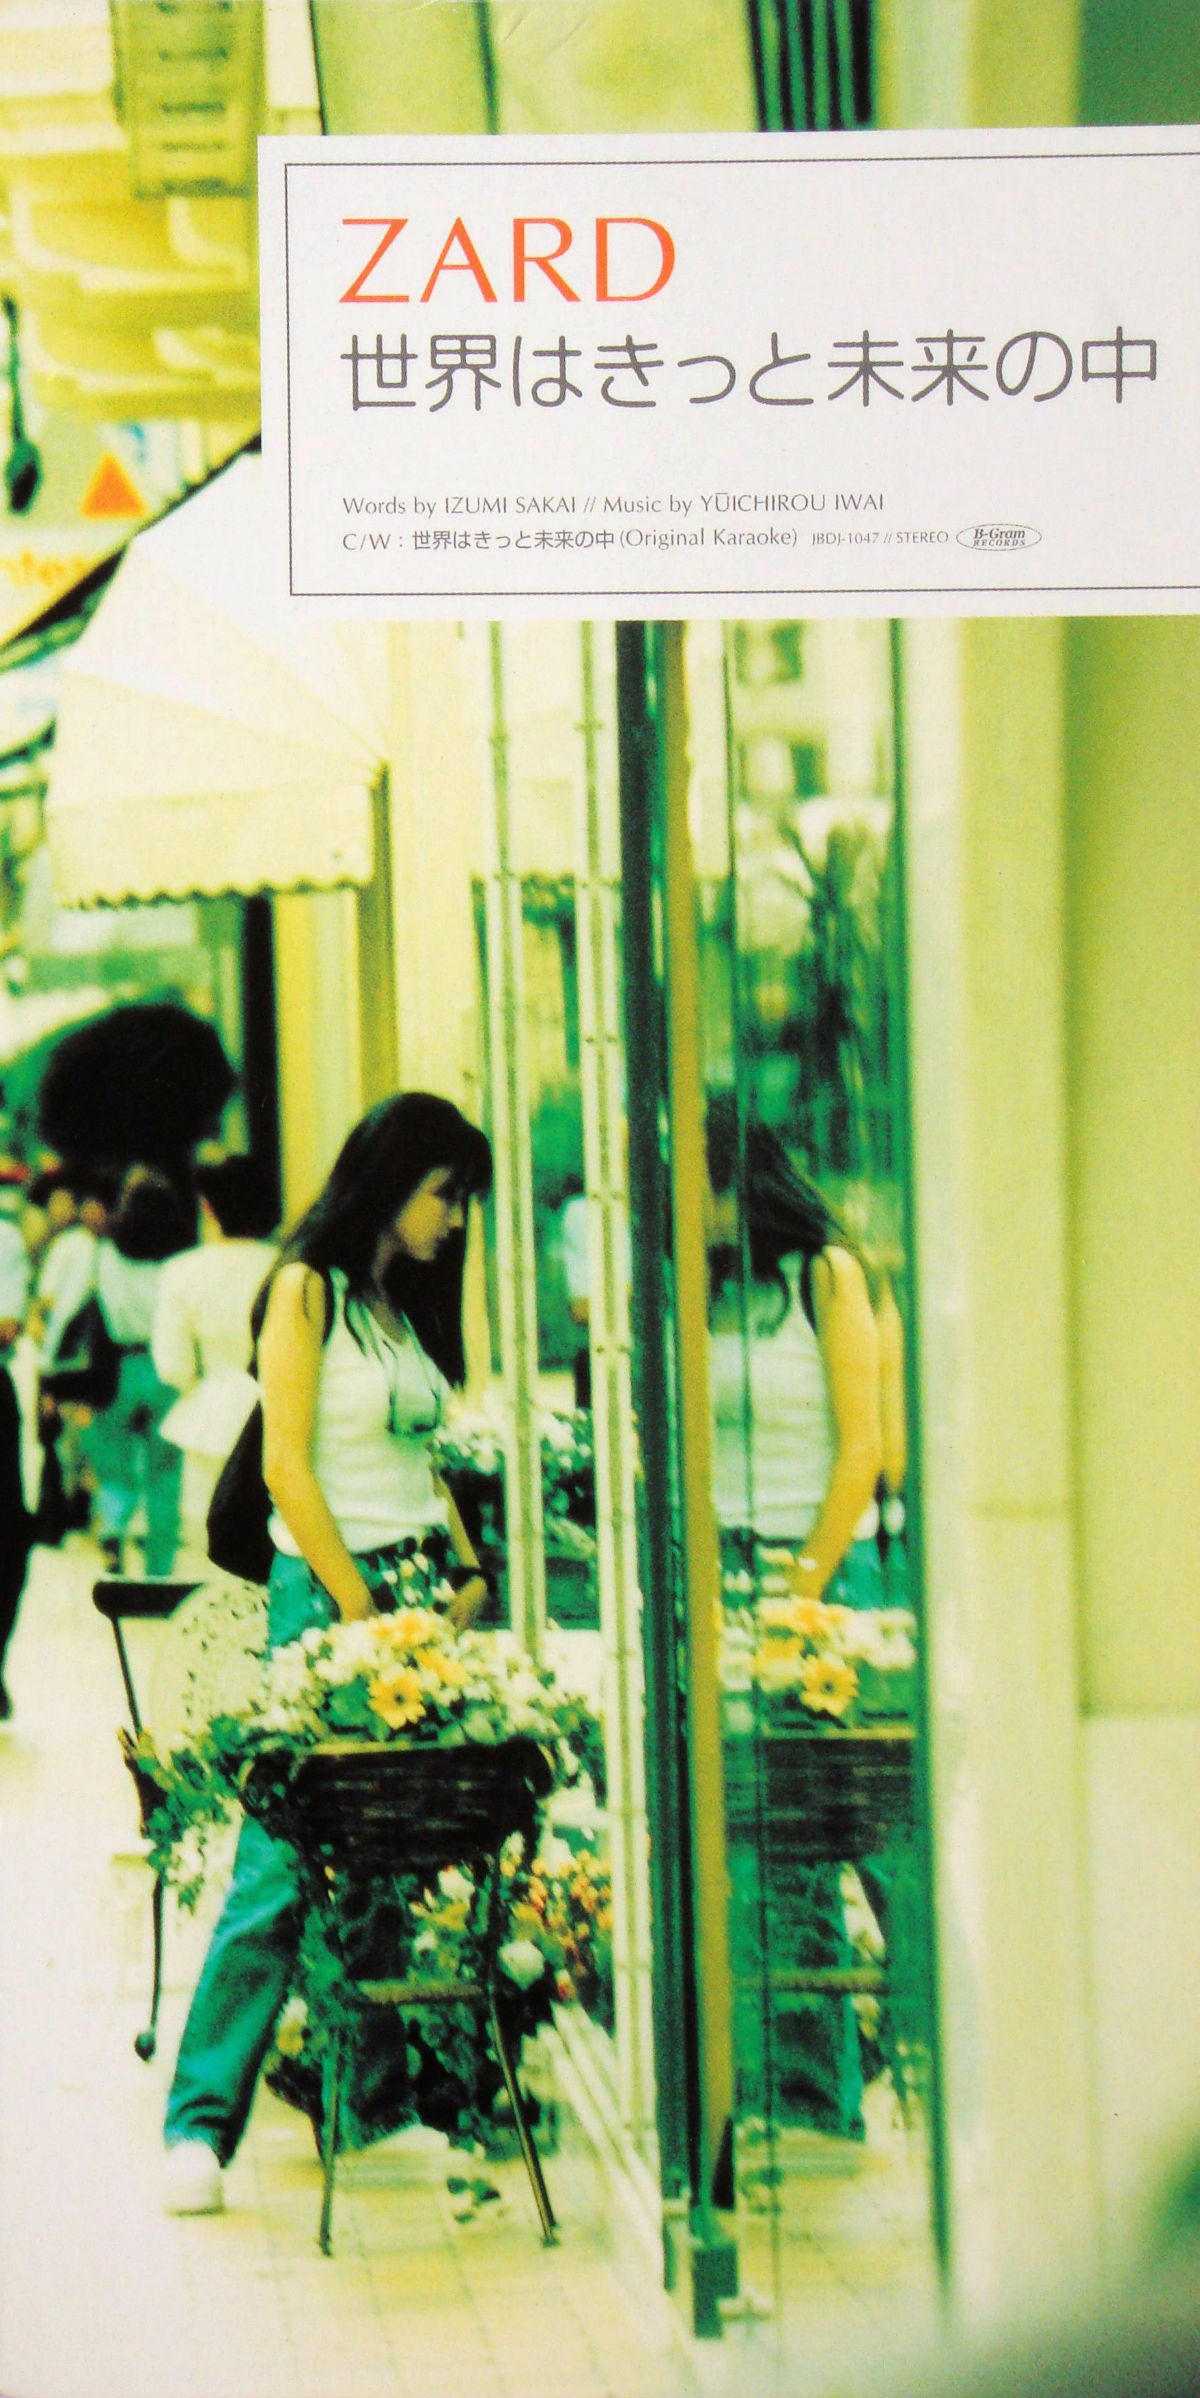
\includegraphics[width=0.3\textwidth]{S29.jpg}}

\large{

\ruby{落}{お}ちこんだ\ruby{時}{とき}も

\ruby{何}{なに}を\ruby{言}{い}っていいか わからない\ruby{時}{とき}も

\ruby{声}{こえ}が\ruby{聴}{き}きたくて…

\ruby{信号}{しんごう}が\ruby{青}{あお}に\ruby{変}{か}わった\ruby{瞬間}{しゅんかん}

\ruby{強気}{つよき}が\ruby{吹}{ふ}きとんだ

\ruby{好}{す}きになれば \ruby{欠点}{けってん}も\ruby{見}{み}えなくなる

\ruby{媚}{こ}びない\ruby{人}{ひと}だから \ruby{信}{しん}じてる
\\

\ruby{世界}{せかい}はきっと\ruby{未来}{みらい}の\ruby{中}{なか}

\ruby{白}{しろ}い\ruby{夏}{なつ}の\ruby{扉}{とびら}\ruby{開}{あ}けて

すべてはきっと Ah woo \ruby{輝}{かがや}く

\ruby{愛}{いと}しいあなたのために
\\

\ruby{無難}{ぶなん}な\ruby{道}{みち}なら いくらでもあるけど

\ruby{今}{いま}はあなた\ruby{以外}{いがい}\ruby{考}{かんが}えられない

\ruby{胃}{い}が\ruby{痛}{いた}くなるほど こんなにはまるなんて

\ruby{価値観}{かちかん}は\ruby{吹}{ふ}き\ruby{飛}{と}んだ!

あなたが\ruby{疑}{うたが}う \ruby{私}{わたし}の\ruby{ココロ}{心}は

きっと \ruby{私}{わたし}の\ruby{迷}{まよ}いなのです
\\

\ruby{世界}{せかい}はきっと\ruby{未来}{みらい}の\ruby{中}{なか}

Car FM が\ruby{海}{うみ}に\ruby{響}{ひび}く

\ruby{時}{とき}が\ruby{経}{た}つのが Ah woo \ruby{速}{はや}いね

\ruby{最初}{さいしょ}の\ruby{頃}{ころ} そうだった\ruby{様}{よう}に
\\

\ruby{風}{かぜ}の\ruby{パワー}{Power}\ruby{何}{なに}かを\ruby{伝}{つた}えたい

でも\ruby{言葉}{ことば}じゃ\ruby{伝}{つた}わらない

\ruby{世界}{せかい}はきっと Ah woo \ruby{輝}{かがや}く

\ruby{決断}{けつだん}のその\ruby{時期}{とき}が\ruby{来}{き}たよね

}

\hypertarget{9_8}{}
\section{ hero}
\large{

\ruby{初}{はじ}めて \ruby{会}{あ}った ときから

\ruby{家族}{かぞく}のような\ruby{気}{き}がしていた

お\ruby{金}{かね}では\ruby{買}{か}えない

\ruby{大事}{だいじ}なものを \ruby{君}{きみ}にあげるよと

kiss me tonight
\\

\ruby{風}{かぜ}の\ruby{音}{おと}が\ruby{目}{め}を\ruby{閉}{と}じると

\ruby{体}{からだ}で\ruby{聞}{き}こえるよ

あなただけが \ruby{私}{わたし}の\ruby{ヒーロー}{hero}だから

\ruby{小}{すこ}しだけ\ruby{笑}{わら}って \ruby{小}{すこ}しだけ\ruby{泣}{な}けば

\ruby{私達}{わたしたち} ふたり いっしょ なら

\ruby{雲}{くも}が\ruby{晴}{は}れてゆく
\\

\ruby{私}{わたし}には\ruby{感}{かん}じるの

あなたが \ruby{泣}{な}きたい \ruby{時}{とき}… なんどなく

みんなを\ruby{照}{て}らす まるで \ruby{魔法}{まほう}の… like a magic

いつも うつむくばかりの\ruby{日}{ひ}にサヨナラ
\\

あの \ruby{自動}{じどう}\ruby{販売機}{はんばいき}まで

せーの\ruby{走}{はし}ってみよう

あなただけが \ruby{私}{わたし}の\ruby{ヒーロー}{hero}だから

\ruby{小}{すこ}しだけ\ruby{笑}{わら}って \ruby{小}{すこ}しだけ\ruby{傷}{きず}ついて

\ruby{私達}{わたしたち} ふたり いっしょ なら

\ruby{虹}{にじ}がかかるよ
\\

\ruby{風}{かぜ}の\ruby{音}{おと}が\ruby{目}{め}を\ruby{閉}{と}じると

\ruby{体}{からだ}で\ruby{聞}{き}こえるよ

あなただけが \ruby{私}{わたし}の\ruby{ヒーロー}{hero}だから

\ruby{小}{すこ}しだけ\ruby{笑}{わら}って \ruby{小}{すこ}しだけ\ruby{泣}{な}けば

\ruby{私達}{わたしたち} ふたり いっしょ なら

\ruby{雲}{くも}が\ruby{晴}{は}れてゆく
\\

\ruby{雲}{くも}が\ruby{晴}{は}れてゆく

}

\hypertarget{9_9}{}
\section{ 時間(とき)の翼}
\large{

\ruby{時間}{とき}の\ruby{翼}{つばさ}で\ruby{蒼}{あお}い\ruby{夕暮}{ゆうぐれ}を

\ruby{手}{て}を \ruby{繫}{つな}いで \ruby{歩}{ある}いたら

\ruby{温}{ぬく}もりが つたわる

\ruby{今}{いま}だけは\ruby{世界}{せかい}でたった\ruby{二人}{ふたり}だけ

\ruby{信}{しん}じる\ruby{気持}{きもち}

とり\ruby{戻}{もど}して\ruby{都会}{とかい}を\ruby{行}{ゆ}く\ruby{風}{かぜ}のように
\\

\parpic[r]{
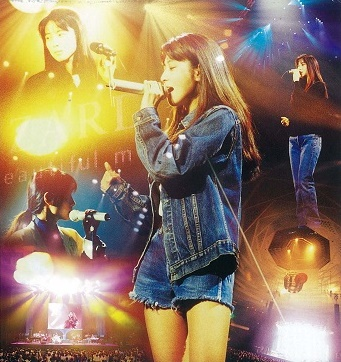
\includegraphics[width=0.4\textwidth]{P11.jpg}}
あれからぼくらは\ruby{出会}{であ}った
\\

\ruby{時間}{とき}の\ruby{翼}{つばさ}で\ruby{青}{あお}い\ruby{夕暮}{ゆうぐれ}を

\ruby{手}{て}を \ruby{繫}{つな}いで \ruby{歩}{ある}いたら

\ruby{温}{ぬく}もりが つたわる

\ruby{時間}{とき}の\ruby{翼}{つばさ}で\ruby{赤}{あか}い\ruby{夕燒}{ゆうやけ}を

くたくたになりながら

\ruby{都会}{とかい}を行く\ruby{風}{かぜ}のように

}

{ \ }



\chapter{Album 10}
\thispagestyle{empty} %本页頁碼空白
\vspace{-16mm}
\LARGE {止まっていた時計が今動き出した}

\normalsize{JBCJ-9008 2004.1.28 \ release}
\\

\vspace{-5mm}

\parpic[l]{
\pichskip{6em}

\includegraphics[width=0.4\textwidth]{10.jpg}}

\small{\hyperlink{10_0}{1.明日を夢見て}}

\tiny{作詞:坂井泉水 \ 作曲:大野愛果 \ 編曲:小林哲}

\small{\hyperlink{10_1}{2.時間(とき)の翼}}

\tiny{作詞:坂井泉水 \ 作曲:大野愛果 \ 編曲:小林哲}

\small{\hyperlink{10_2}{3.もっと近くで君の橫顏見ていたい}}

\tiny{作詞:坂井泉水 \ 作曲:大野愛果 \ 編曲:池田大介}

\small{\hyperlink{10_3}{4.pray}}

\tiny{作詞:坂井泉水 \ 作曲:徳永暁人 \ 編曲:小林哲}

\small{\hyperlink{10_4}{5.出逢いそして別れ}}

\tiny{作詞:坂井泉水 \ 作曲:春畑道哉 \ 編曲:春畑道哉/池田大介}

\small{\hyperlink{10_5}{6.止まっていた時計が今動き出した}}

\tiny{作詞:坂井泉水 \ 作曲:中村由利 \ 編曲:徳永暁人}

\small{\hyperlink{10_6}{7.瞳閉じて}}

\tiny{作詞:坂井泉水 \ 作曲:大野愛果 \ 編曲:徳永暁人}

\small{\hyperlink{10_7}{8.さわやかな君の気持ち(Album Ver.)}}

\tiny{作詞:坂井泉水 \ 作曲/編曲:徳永暁人}

\small{\hyperlink{10_8}{9.愛であなたを救いましょう}}

\tiny{作詞:坂井泉水 \ 作曲:栗林誠一郎 \ 編曲:明石昌夫}

\small{\hyperlink{10_9}{10.天使のような笑顏で}}

\tiny{作詞:坂井泉水 \ 作曲:大野愛果 \ 編曲:徳永暁人}

\small{\hyperlink{10_10}{11.悲しいほど今日は雨でも}}

\tiny{作詞:坂井泉水 \ 作曲:大野愛果 \ 編曲:小林哲}

\small{ \ }

\tiny{ \ }

\small{ \ }

\tiny{ \ }

\clearpage


\hypertarget{10_0}{}
\section{ 明日を夢見て}

\parpic[r]{

\includegraphics[width=0.4\textwidth]{S35.jpg}}

\large{

\ruby{夢}{ゆめ}のように 

\ruby{選}{えら}びながら

この\ruby{毎日}{まいにち}を 

\ruby{生}{い}きていけたなら

もしもあの\ruby{時}{とき} 

\ruby{違}{ちが}う\ruby{決断}{けつだん}をしていたら

\ruby{今頃}{いまごろ}\ruby{私達}{ふたり}\ruby{幸}{しあわ}せに

\ruby{笑}{わら}っていられたのかな
\\

\ruby{本当}{ほんとう}は\ruby{誰}{だれ}にも \ruby{心}{こころ}\ruby{開}{ひら}けない

\ruby{週末}{しゅうまつ}の \ruby{賑}{にぎ}わう\ruby{街}{まち}

わけもなく\ruby{涙}{なみだ}が\ruby{出}{で}た

I need you
\\

\ruby{明日}{あした}を\ruby{夢見}{ゆめみ}て \ruby{強}{つよ}がっては

\ruby{夢}{ゆめ}の\ruby{入}{い}り\ruby{口}{くち}に やっとせっかくたったのに

\ruby{誰}{だれ}にも \ruby{言}{い}えないことがあっても

\ruby{皆}{みな}それぞれだけど

お\ruby{互}{たが}い\ruby{思}{おも}いやりながら \ruby{生}{い}きている
\\

\ruby{君}{きみ}の\ruby{電話}{でんわ}の\ruby{声}{こえ}を\ruby{聴}{き}くと

\ruby{泣}{な}きたくなる \ruby{強}{つよ}い\ruby{私}{わたし}でも

\ruby{傷}{きず}つけ\ruby{合}{あ}って それでも また\ruby{会}{あ}いたくて

いつだってピリオドと\ruby{背中}{せなか}\ruby{合}{あ}わせ
\\

\ruby{君}{きみ}は\ruby{返事}{へんじ}に\ruby{困}{こま}っていたね

\ruby{隠}{かく}せないその\ruby{表情}{かお}を\ruby{思}{おも}い\ruby{出}{だ}すたびに... I miss you
\\

\ruby{明日}{あした}を\ruby{夢見}{ゆめみ}て \ruby{君}{きみ}のこと

\ruby{信}{しん}じていたいよ \ruby{寄}{よ}り\ruby{道}{みち}もしたけど

\ruby{明日}{あした}を\ruby{夢見}{ゆめみ}て \ruby{君}{きみ}のこと

\ruby{見}{み}つめていたいよ

また\ruby{僅}{わず}かに \ruby{木漏}{こも}れ\ruby{日}{び}が\ruby{揺}{ゆ}れるから
\\

\ruby{二人}{ふたり}の\ruby{冷}{さ}めた\ruby{誤解}{ごかい} \ruby{溶}{と}かしたい

\ruby{信}{しん}じていたいよ \ruby{寄}{よ}り\ruby{道}{みち}もしたけど

\ruby{明日}{あした}を\ruby{夢見}{ゆめみ}て この\ruby{想}{おも}い

\ruby{時々}{ときどき}\ruby{切}{せつ}なくて \ruby{押}{お}しつぶされそうになるけど

\ruby{明日}{あした}を\ruby{夢見}{ゆめみ}て \ruby{君}{きみ}のこと

\ruby{見}{み}つめていたいよ

まだ\ruby{僅}{わず}かに \ruby{木漏}{こも}れ\ruby{日}{び}が\ruby{揺}{ゆ}れるから

}

\hypertarget{10_1}{}
\section{ 時間の翼}
\large{

\ruby{口笛}{くちぶえ}\ruby{吹}{ふ}くと クスッと\ruby{君}{きみ}が\ruby{笑}{わら}った

\ruby{今日}{きょう}\ruby{一}{いち}\ruby{日}{にち}あった\ruby{事}{こと} いろいろ\ruby{話}{はな}したね

\ruby{夏}{なつ}が\ruby{過}{す}ぎて \ruby{冬}{ふゆ}の\ruby{季節}{きせつ}がやって\ruby{来}{き}ても

\ruby{君}{きみ}と\ruby{二人}{ふたり}で こうしていたい
\\

\ruby{他人}{ひと}の\ruby{言葉}{ことば}に\ruby{惑}{まど}わされちゃいけない

「\ruby{幸}{しあわ}せ\ruby{」語}{かた}る\ruby{人}{ひと}\ruby{程}{ほど} ほんとは\ruby{寂}{さび}しいんだよ
\\

\ruby{時間}{とき}の\ruby{翼}{つばさ}で \ruby{蒼}{あお}い\ruby{夕暮}{ゆうぐ}れを

ビルの\ruby{灯}{あかり}かりが ひとつずつもうすぐついていく

\ruby{時間}{とき}の\ruby{翼}{つばさ}で \ruby{蒼}{あお}い\ruby{夕暮}{ゆうぐ}れを

くたくたになりながら \ruby{都会}{とかい}を\ruby{行}{い}く\ruby{風}{かぜ}のように
\\

\ruby{諦}{あきら}めるのは まだ ズッと\ruby{先}{さき}でいいじゃない

\ruby{真剣}{しんけん}に\ruby{生}{い}きてる アナタが\ruby{好}{す}き
\\

\ruby{町}{まち}の\ruby{雑音}{ざつおん}がみるみるうちに

\ruby{交差点}{こうさてん}の\ruby{向}{む}こう\ruby{側}{がわ}に \ruby{吸}{す}い\ruby{込}{こ}まれていく
\\

\ruby{時間}{とき}の\ruby{翼}{つばさ}で \ruby{蒼}{あお}い\ruby{夕暮}{ゆうぐ}れを

\ruby{手}{て}を\ruby{繋}{つな}いで\ruby{歩}{ある}いたら \ruby{温}{ぬく}もりが\ruby{伝}{つた}わる

\ruby{今}{いま}だけは \ruby{世界}{せかい}でたった\ruby{二人}{ふたり}だけ

\ruby{信}{しん}じる\ruby{気持}{きも}ち とり\ruby{戻}{もど}して \ruby{都会}{とかい}を\ruby{行}{い}く\ruby{風}{かぜ}のように
\\

あれから ぼくらは \ruby{出会}{であ}った
\\

\ruby{時間}{とき}の\ruby{翼}{つばさ}で \ruby{蒼}{あお}い\ruby{夕暮}{ゆうぐ}れを

\ruby{手}{て}を\ruby{繋}{つな}いで\ruby{歩}{ある}いたら \ruby{温}{ぬく}もりが\ruby{伝}{つた}わる

\ruby{時間}{とき}の\ruby{翼}{つばさ}で \ruby{赤}{あか}い\ruby{夕焼}{ゆうや}けを

くたくたになりながら \ruby{都会}{とかい}を\ruby{行}{い}く\ruby{風}{かぜ}のように

}

\hypertarget{10_2}{}
\section{ もっと近くで君の横顔見ていたい}

\parpic[r]{
\includegraphics[width=0.4\textwidth]{S37.jpg}}

\large{

もっと\ruby{近}{ちか}くで\ruby{君}{きみ}の\ruby{横顔}{よこがお}\ruby{見}{み}ていたい

\ruby{月}{つき}を\ruby{浮}{う}かべて\ruby{夜}{よる}を\ruby{語}{かた}り\ruby{明}{あ}かそうよ

ずっと\ruby{見}{み}えずにいた 

\ruby{素顔}{すがお}\ruby{探}{さが}していたの

\ruby{希望}{きぼう}と\ruby{安}{やす}らぎをくれた\ruby{君}{きみ}とは

\ruby{想}{おも}いも\ruby{尽}{つ}きない Um... 

\ruby{夢}{ゆめ}を\ruby{追}{お}っていたのは

そう \ruby{遠}{とお}い\ruby{記憶}{きおく}
\\

\ruby{離}{はな}れる\ruby{程}{ほど}につのる\ruby{想}{おも}い

あの\ruby{空}{そら}へ\ruby{届}{とど}くといいな

\ruby{壊}{こわ}れてしまったオモチャのように

\ruby{色}{いろ}を\ruby{失}{うしな}ってしまった
\\

\ruby{心}{こころ}\ruby{塞}{ふさ}ぐ\ruby{日}{ひ}はいつも\ruby{君}{きみ}が\ruby{傍}{そば}となりで\ruby{笑}{わら}ってくれたよね
\\

もっと\ruby{近}{ちか}くで\ruby{君}{きみ}の\ruby{横顔}{よこがお}\ruby{見}{み}ていたい

\ruby{月}{つき}を\ruby{浮}{う}かべて\ruby{夜}{よる}を\ruby{語}{かた}り\ruby{明}{あ}かそうよ

たった\ruby{一言}{ひとこと}で \ruby{二人}{ふたり}の\ruby{世界}{せかい}が\ruby{謎}{なぞ}めく

ときめきと\ruby{眠}{ねむ}れぬ\ruby{夜}{よる}は\ruby{君}{きみ}との

\ruby{想}{おも}いも\ruby{尽}{つ}きない Um... \ruby{夢}{ゆめ}を\ruby{追}{お}っているなら

そう \ruby{光}{ひか}り\ruby{始}{はじ}める
\\

\ruby{淋}{さび}しさで\ruby{人}{ひと}は\ruby{愛}{あい}に\ruby{苛立}{いらだ}ちをおぼえてゆく

でも\ruby{人}{ひと}は\ruby{淋}{さび}しさで\ruby{強}{つよ}くなってゆくよね
\\

\ruby{遥}{はる}かな\ruby{旅}{たび}をしている \ruby{二人}{ふたり}の\ruby{行}{ゆ}き\ruby{先}{さき}えは \ruby{君}{きみ}に\ruby{委}{ゆだ}ねたい
\\

もっと\ruby{近}{ちか}くで\ruby{君}{きみ}の\ruby{横顔}{よこがお}\ruby{見}{み}ていたい

コンクリートの\ruby{壁}{かべ} \ruby{枯葉}{かれは}\ruby{散}{ち}る\ruby{夕暮}{ゆうぐ}れ\ruby{二人}{ふたり}\ruby{歩}{ある}こうよ

せつなくて せつなくて \ruby{会}{あ}いたい

\ruby{私}{わたし}を\ruby{照}{て}らす\ruby{一点}{ひとつ}の\ruby{灯}{あか}り

\ruby{希望}{きぼう}と\ruby{安}{やす}らぎをくれた\ruby{君}{きみ}とは

\ruby{想}{おも}いも\ruby{尽}{つ}きない Um... \ruby{華}{はな}やいだ\ruby{季節}{きせつ}は

そう \ruby{遠}{とお}い\ruby{記憶}{きおく}

}

\hypertarget{10_3}{}
\section{ Pray}
\large{

\ruby{穏}{おだ}やかな\ruby{日々}{ひび}

それは\ruby{二人}{ふたり}がいつしか\ruby{失}{しつ}くしてしまったもの

あの\ruby{懐}{なつ}かしい\ruby{故郷}{こきょう}へ

いつか\ruby{帰}{かえ}りたいと

\ruby{雨}{あめ}の\ruby{日}{ひ}はそう\ruby{願}{ねが}う
\\

\ruby{素敵}{すてき}な\ruby{思}{おも}い\ruby{出}{で}だけ

\ruby{胸}{むね}にしまっておけたらいいのにと\ruby{祈}{いの}る

いつも\ruby{変}{か}わりなく\ruby{動}{うご}き\ruby{始}{はじ}める\ruby{世界}{せかい}は

すべてがはかない
\\

いつの\ruby{夜}{よ}も

\ruby{信}{しん}じられずに

きっかけ\ruby{待}{ま}っていた

\ruby{秘密}{ひみつ}の

つらい\ruby{愛}{あい}も

つらい\ruby{過去}{かこ}も

\ruby{今}{いま}はお\ruby{休}{やす}み
\\

あの\ruby{頃}{ころ}

\ruby{二人}{ふたり}で

\ruby{海}{うみ}を\ruby{眺}{なが}めているだけで

とてもとても

\ruby{幸}{しあわ}せだったよね

ただとなりにいて

\ruby{君}{きみ}の\ruby{話}{はなし}を\ruby{聞}{き}いているだけだったけど

\ruby{後戻}{あともど}り\ruby{出来}{でき}ない

きっと\ruby{決}{き}まっていて

\ruby{赤}{あか}い\ruby{糸}{いと}のあなたに\ruby{出会}{であ}えたの

you're my dream
\\

この\ruby{永}{なが}い\ruby{冬}{ふゆ}が\ruby{溶}{と}けて

\ruby{再}{ふたた}び\ruby{行}{い}き\ruby{場}{ば}のない\ruby{想}{おも}いは

oh

じっとしていると\ruby{寂}{さび}しさで\ruby{凍}{こお}りついてしまいそう

You are the only one oh
\\

\ruby{心地}{ここち}\ruby{良}{よ}かった

コーヒーとバーガーで\ruby{何}{なん}\ruby{時間}{じかん}も

いつもいつも

この\ruby{席}{せき}だったよね

まだ\ruby{心}{こころ}の\ruby{準備}{じゅんび}さえ

できる\ruby{時間}{じかん}なかったけど

\ruby{後戻}{あともど}りは\ruby{出来}{でき}ない

きっと\ruby{決}{き}まっていて

\ruby{赤}{あか}い\ruby{糸}{いと}のあなたに\ruby{出会}{であ}えたの

you're my DREAM !

}

\hypertarget{10_4}{}
\section{ 出逢いそして別れ}
\large{

I wanna run to you

その\ruby{夢}{ゆめ}は\ruby{叶}{かな}うの?

\ruby{見慣}{みな}れぬ\ruby{街}{まち}

\ruby{空}{そら}に\ruby{向}{む}かって

\ruby{傷}{きず}ついても

\ruby{一歩}{いっぽ}\ruby{前進}{ぜんしん}しなきゃね
\\

この\ruby{楽園}{らくえん}に

\ruby{自由}{じゆう}が\ruby{欲}{ほ}しいという

そして\ruby{君}{きみ}は

また\ruby{新}{あたら}しい\ruby{恋}{こい}に\ruby{焦}{こ}がれてゆくの

Oh, heart break, my love
\\

いつの\ruby{間}{ま}にか\ruby{一緒}{いっしょ}に

\ruby{夢見}{ゆめみ}\ruby{続}{つづ}けてきたこと

\ruby{忘}{わす}れていったね

\ruby{気}{き}づくときには\ruby{遠}{とお}くて
\\

\ruby{出逢}{であ}い

そして\ruby{別}{わか}れ

\ruby{時間}{じかん}が\ruby{頬}{ほほ}を\ruby{撫}{な}でる

いつまでも

\ruby{忘}{わす}れないで

ずっとずっと\ruby{愛}{あい}されていたこと

Give me a smile more... その\ruby{先}{さき}に\ruby{何}{なに}が\ruby{起}{お}こるかなんて

わからない

\ruby{命}{いのち}\ruby{在}{あ}る\ruby{限}{かぎ}り

それがきっとone wayだからね

I'll always love you
\\

You can go anywhere

\ruby{夜明}{よあ}けはやって\ruby{来}{く}る

あなたにも

\ruby{私}{わたし}にも

\ruby{確}{たし}かなものはなにもないけど

Oh, stand up to yourself
\\

\ruby{急}{いそ}いで\ruby{駆}{か}け\ruby{抜}{ぬ}けた\ruby{旅路}{たびじ}

\ruby{思}{おも}い\ruby{出}{で}は

slowly

\ruby{二人}{ふたり}つつみ\ruby{込}{こ}む

\ruby{月}{つき}\ruby{灯}{あかり}かりは\ruby{変}{か}わらない
\\

\ruby{出逢}{であ}い

そして\ruby{別}{わか}れ

\ruby{時間}{じかん}が\ruby{頬}{ほほ}を\ruby{撫}{な}でる

\ruby{運命}{うんめい}のいたずらでも\ruby{忘}{わす}れないで

\ruby{愛}{あい}されていたこと

Give me a smile more... その\ruby{先}{さき}に\ruby{何}{なに}が\ruby{起}{お}こるかなんて

わからない

\ruby{命}{いのち}\ruby{在}{あ}る\ruby{限}{かぎ}り

それがきっとone wayだからね

I wanna keep on goin'my way
\\

\ruby{出逢}{であ}いそして\ruby{別}{わか}れ

\ruby{涙}{なみだ}が\ruby{頬}{ほほ}を\ruby{伝}{つた}う

\ruby{風}{かぜ}が\ruby{吹}{ふ}く

ねじれた\ruby{愛}{あい}

もうこれ\ruby{以上}{いじょう}\ruby{何}{なに}も\ruby{要}{い}らない

\ruby{出逢}{であ}い

そして\ruby{思}{おも}い\ruby{通}{どお}りに

\ruby{生}{い}きてごらん

\ruby{命}{いのち}\ruby{在}{あ}る\ruby{限}{かぎ}り

それが\ruby{希望}{きぼう}one wayだからね

Give me a smile more... その\ruby{先}{さき}に\ruby{何}{なに}が\ruby{起}{お}こるかなんて

わからない

\ruby{命}{いのち}\ruby{在}{あ}る\ruby{限}{かぎ}り

それがきっとone wayだからね

I'll always love you

}

\hypertarget{10_5}{}
\section{ 止まっていた時計が今動き出した}
\large{

まためぐり\ruby{合}{あ}う\ruby{春}{はる}を\ruby{待}{ま}っている

\ruby{時}{とき}よつづれ

そして\ruby{人}{ひと}は\ruby{皆}{みな}

\ruby{僅}{わず}かな\ruby{誇}{ほこ}りと\ruby{運命}{うんめい}を\ruby{感}{かん}じている

\ruby{此処}{ここ}には

\ruby{過去}{かこ}も\ruby{未来}{みらい}もない

\ruby{今}{いま}しかない

まわり\ruby{道}{みち}も

\ruby{意味}{いみ}がある\ruby{修行}{おしえ}と\ruby{気付}{きづ}く\ruby{日}{ひ}が\ruby{来}{く}る

きっとどこかへと

つながっている

\ruby{冷}{つめ}たい\ruby{石}{いし}の\ruby{上}{うえ}を\ruby{歩}{ある}く

\ruby{靴音}{くつおと}が\ruby{懐}{なつ}かしいよね

\ruby{許}{ゆる}せなかった\ruby{幼}{おさな}い\ruby{日}{ひ}

どうかせめて\ruby{前途}{ぜんと}ある\ruby{未来}{みらい}に...
\\

\ruby{君}{きみ}の\ruby{胸}{むね}の\ruby{中}{なか}に

\ruby{何}{なに}も\ruby{持}{も}たずに\ruby{今}{いま}

\ruby{飛}{と}び\ruby{込}{こ}んでいけるなら

ねえいきたいよ

\ruby{何処}{どこ}か\ruby{果}{は}てまで

\ruby{悲}{かな}しい\ruby{雨}{あめ}が\ruby{心}{こころ}を\ruby{濡}{ぬ}らしてゆく

\ruby{止}{と}まっていた\ruby{時計}{とけい}が\ruby{今}{いま}\ruby{動}{うご}き\ruby{出}{だ}すから
\\

\ruby{君}{きみ}と\ruby{眠}{ねむ}る\ruby{時間}{じかん}

\ruby{他人}{ひと}には\ruby{見}{み}せない\ruby{顔}{かお}

だんだん\ruby{君}{きみ}との\ruby{思}{おも}いでも\ruby{薄}{うす}れていくよ

\ruby{哀}{かな}しい\ruby{雨}{あめ}が\ruby{心}{こころ}を\ruby{濡}{ぬ}らしてゆく

\ruby{止}{と}まっていた\ruby{時計}{とけい}が\ruby{今}{いま}

\ruby{動}{うご}く
\\

\ruby{君}{きみ}の\ruby{胸}{むね}の\ruby{中}{なか}

\ruby{何}{なに}も\ruby{持}{も}たずに

\ruby{今}{いま}

\ruby{飛}{と}び\ruby{込}{こ}んでいけるなら

ねえ

いきたいよ

\ruby{何処}{どこ}か\ruby{果}{は}てまで

\ruby{悲}{かな}しい\ruby{雨}{あめ}が\ruby{心}{こころ}を\ruby{濡}{ぬ}らしてゆく

\ruby{止}{と}まっていた\ruby{時計}{とけい}が\ruby{今}{いま}\ruby{動}{うご}き\ruby{出}{だ}したよ
\\

\ruby{止}{と}まっていた\ruby{時計}{とけい}が\ruby{今}{いま}\ruby{動}{うご}き\ruby{出}{だ}すから

}

\hypertarget{10_6}{}
\section{ 瞳閉じて}

\large{

\ruby{心臓}{ココロ}を \ruby{強}{つよ}く\ruby{叩}{たた}いたり

\ruby{溺}{おぼ}れる\ruby{様}{よう}に \ruby{涙}{なみだ}を\ruby{流}{なが}したい

\ruby{輝}{かがや}ける\ruby{未来}{みらい}に\ruby{期待}{きたい}を\ruby{抱}{いだ}いていた あの\ruby{日}{ひ}は

ポケットの\ruby{奥}{おく}に しまい\ruby{込}{こ}んだ
\\

\ruby{夢}{ゆめ}の\ruby{中}{なか}で よく\ruby{見知}{みし}らぬ\ruby{街}{まち}を

さまよっているの
\\

\parpic[r]{
\includegraphics[width=0.4\textwidth]{S36.jpg}}

\ruby{瞳}{ひとみ}\ruby{閉}{と}じて \ruby{二人}{ふたり}つながってる\ruby{事}{こと}を

\ruby{私}{わたし}に \ruby{伝}{つた}えてほしい

\ruby{涙}{なみだ}を\ruby{流}{なが}す\ruby{姿}{すがた}は \ruby{誰}{だれ}にも\ruby{見}{み}せない

\ruby{雲}{くも}の\ruby{色}{いろ}が\ruby{違}{ちが}うわ

\ruby{雲}{くも}の\ruby{色}{いろ}が \ruby{今日}{きょう}は\ruby{明}{あか}るい
\\

むき\ruby{出}{だ}しのままの \ruby{君}{きみ}の\ruby{心}{こころ}は

どこに\ruby{行}{い}ってしまったの あの\ruby{日}{ひ}から

パズルのようにピースはめ\ruby{込}{こ}み \ruby{季節}{きせつ}が\ruby{変}{か}わるたび

いつの\ruby{日}{ひ}か\ruby{奇蹟}{きせき}がおきて
\\

\ruby{私}{わたし}だけが\ruby{孤独}{こどく}なの? why?

\ruby{形}{かたち}だけの words of love
\\

\ruby{瞳}{ひとみ}\ruby{閉}{と}じて \ruby{君}{きみ}の\ruby{感}{かん}じてるものを

\ruby{私}{わたし}に \ruby{伝}{つた}えてほしい

\ruby{不思議}{ふしぎ}な\ruby{力}{ちから}が この\ruby{世}{よ}にあって

\ruby{君}{きみ}が\ruby{笑}{わら}うと\ruby{嬉}{うれ}しい

\ruby{君}{きみ}が\ruby{笑}{わら}うと とても\ruby{眩}{まぶ}しい
\\

\ruby{瞳}{ひとみ}\ruby{閉}{と}じて \ruby{今}{いま}もつながってる\ruby{事}{こと}を

\ruby{私}{わたし}に \ruby{伝}{つた}えてほしい

\ruby{時々}{ときどき}\ruby{逃}{に}げ\ruby{出}{だ}したくなる \ruby{憶病者}{おくびょう}

\ruby{雲}{くも}の\ruby{流}{なが}れが\ruby{違}{ちが}うわ

\ruby{雲}{くも}の\ruby{流}{なが}れが \ruby{今日}{きょう}は\ruby{速}{はや}い
\\

Ah \ruby{君}{きみ}の\ruby{感}{かん}じてるものを

\ruby{私}{わたし}に \ruby{伝}{つた}えてほしい

\ruby{不思議}{ふしぎ}な\ruby{力}{ちから}が

この\ruby{世}{よ}にあって

\ruby{君}{きみ}が\ruby{笑}{わら}うと\ruby{嬉}{うれ}しい

\ruby{君}{きみ}が\ruby{笑}{わら}うと とても\ruby{眩}{まぶ}しい

}

\hypertarget{10_7}{}
\section{ さわやかな君の気持ち(Album Ver.)}

\parpic[r]{
\includegraphics[width=0.4\textwidth]{S34.jpg}}

\large{

\ruby{比}{くら}べることなんて \ruby{無意味}{むいみ}なのにね

いつも \ruby{周囲}{まわり}と\ruby{比}{くら}べては ヘコんで

\ruby{波}{なみ}の\ruby{音}{おと}が\ruby{心地}{ごこち}よかった

\ruby{私}{わたし}を\ruby{見}{み}る その\ruby{瞳}{ひとみ}は\ruby{強}{つよ}く

\ruby{君}{きみ}の\ruby{胸}{むね}の\ruby{中}{なか}に\ruby{抱}{だ}かれ hold me

\ruby{夏}{なつ}の\ruby{日差}{ひざ}しの\ruby{中}{なか}

\ruby{私}{わたし}の\ruby{手}{て}に\ruby{抱}{だ}かれた hold you

\ruby{戻}{もど}るはずもない
\\

さわやかな\ruby{君}{きみ}の\ruby{気持}{きも}ちで\ruby{歩}{ある}いた

ときには \ruby{先}{さき}が\ruby{見}{み}えなくて

\ruby{今日}{きょう}もまた\ruby{一日}{いちにち} \ruby{迷}{まよ}わない\ruby{笑顔}{えがお}で

どうしてだろう…

\ruby{互}{たが}いにとって\ruby{言葉}{ことば}は\ruby{不自然}{ふしぜん}になってゆくよ

\ruby{駆}{か}け\ruby{抜}{ぬ}けた\ruby{季節}{きせつ}だけ

ずっと あなたを\ruby{見}{み}ていたよ
\\

\ruby{矛盾}{むじゅん}と\ruby{エゴ}{ego}の\ruby{良心}{りょうしん}の\ruby{呵責}{かしゃく}

\ruby{何故}{なぜ} \ruby{夢}{ゆめ}のように ほどけていくの?

\ruby{電話}{でんわ}したのは call you ただ\ruby{好}{す}きと\ruby{伝}{つた}えたいから

つなぎとめて call me おく\ruby{手段}{しゅだん}と\ruby{思}{おも}いたくない
\\

あの\ruby{時}{とき} \ruby{君}{きみ}の\ruby{気持}{きも}ちに\ruby{気付}{きづ}いて

ときには\ruby{泣}{な}いてあげたなら…

\ruby{今日}{きょう}もまた\ruby{一日}{いちにち} \ruby{迷}{まよ}わない\ruby{笑顔}{えがお}で

どうしてだろう…

\ruby{空}{そら}の\ruby{青}{あお}さ\ruby{見}{み}るたび

\ruby{口}{くち}に\ruby{出}{だ}すのが\ruby{恐}{こわ}くて

\ruby{駆}{か}け\ruby{抜}{ぬ}けた\ruby{季節}{きせつ}だけ

ずっと あなたを\ruby{見}{み}ていたよ
\\

Did I hear you say you need me?

So very lonely was my heart

I wish those days cloud come back once more

'Cause one they start to light up the sky
\\

さわやかな\ruby{君}{きみ}の\ruby{気持}{きも}ちで\ruby{歩}{ある}いた

\ruby{時}{とき}には \ruby{真実}{さき}が\ruby{見}{み}えなくて

\ruby{今日}{きょう}もまた\ruby{一日}{いちにち} \ruby{迷}{まよ}わない\ruby{笑顔}{えがお}で

Don't you worry why did those days ever have to go?

\ruby{不自然}{ふしぜん}に なってゆくよ

\ruby{駆}{か}け\ruby{抜}{ぬ}けた\ruby{季節}{きせつ}だけ

ずっと アナタを\ruby{見}{み}ていたよ

}

\hypertarget{10_8}{}
\section{ 愛であなたを救いましょう}
\large{

もうあなたが\ruby{嫌}{いや}がるから ピアスもやめたし

ミニスカートだってデートの\ruby{時}{とき}だけ

\ruby{日常}{にちじょう}の\ruby{1週間}{しゅうかん}の\ruby{半分}{はんぶん}は あなたからの\ruby{電話}{でんわ}を\ruby{待}{ま}って

ソワソワ\ruby{部屋}{へや}にこもりきり
\\

\ruby{愛}{あい}であなたを\ruby{救}{すく}いましょう \ruby{優柔不断}{ゆうじゅうふだん}な

あなたの\ruby{考}{かんが}えてることっていったい\ruby{何}{なに}? \ruby{全然}{ぜんぜん}わからない
\\

\ruby{荷物}{にもつ}を\ruby{抱}{かか}え \ruby{毎朝}{まいあさ}ラッシュアワーの\ruby{1日}{にち}が\ruby{始}{はじ}まる Oh No

\ruby{次}{つぎ}から\ruby{次}{つぎ}へと めま\ruby{苦}{くる}しく\ruby{変}{か}わる\ruby{街}{まち}へと\ruby{急}{いそ}ぎ

それでも あなたと\ruby{会}{あ}えない\ruby{日}{ひ}が\ruby{続}{つづ}くと やっぱりさみしい
\\

あなたが\ruby{嫌}{いや}だっていくから

\ruby{女}{おんな}\ruby{友達}{かのじょ}とだって \ruby{旅行}{りょこう}に\ruby{行}{い}かないし

なのに \ruby{週末}{しゅうまつ}は\ruby{私}{わたし}を\ruby{置}{お}いて \ruby{釣}{つ}りに\ruby{行}{い}ってる
\\

\ruby{愛}{あい}であなたを\ruby{救}{すく}いましょう 「いいの\ruby{仕事}{しごと}なら」

\ruby{最初}{さいしょ}から\ruby{誓約}{せいやく}\ruby{書}{しょ}でも\ruby{作}{つく}るんだった ずるい…\ruby{沈黙}{ちんもく}なんて
\\

ぜいたくは\ruby{夢}{ゆめ}を\ruby{少}{すこ}しずつ\ruby{食}{た}べてしまうから Oh No

\ruby{段々}{だんだん}\ruby{想}{おも}いが ああ \ruby{満}{み}たされなくなるよ

それでも あなたと\ruby{一緒}{いっしょ}にいる\ruby{時}{とき}が\ruby{一番}{いちばん}\ruby{楽}{たの}しい

}

\hypertarget{10_9}{}
\section{ 天使のような笑顔で}
\large{

\ruby{天使}{てんし}のような\ruby{笑顔}{えがお}で smile on me
\\

\ruby{季節}{きせつ}のうつろいと\ruby{一緒}{いっしょ}に

\ruby{気持}{きも}ちも\ruby{曖昧}{あいまい}に\ruby{変化}{へんか}してゆくよ

いつかの\ruby{夏}{なつ}は \ruby{遠}{とお}くなるけど
\\

\ruby{君}{きみ}だけのことを

\ruby{何}{なに}より\ruby{大切}{たいせつ}に\ruby{思}{おも}い\ruby{始}{はじ}めたよ
\\

\ruby{天使}{てんし}のような\ruby{笑顔}{えがお}で smile on me

とびきりかわいい\ruby{彼女}{かのじょ}は\ruby{宝物}{ほうもつ}

でも\ruby{胸}{むね}さわぎする \ruby{風}{かぜ}が\ruby{吹}{ふ}くと

\ruby{彼女}{かのじょ}の\ruby{心}{こころ}の\ruby{奥}{おく}は \ruby{誰}{だれ}にも\ruby{分}{わ}からない
\\

\ruby{昨日今日}{きのうきょう}があわただしくて

\ruby{振}{ふ}り\ruby{返}{かえ}ってみる ヒマもない

\ruby{勝}{か}つとか\ruby{負}{ま}けるとか そんな\ruby{小}{ちい}さな\ruby{事}{こと}で

まどわされたくない、ね!
\\

きっかけは\ruby{月並}{つきな}みな\ruby{出来事}{できごと}

いっそ\ruby{甘}{あま}い\ruby{誘惑}{ゆうわく}に \ruby{酔}{よ}ってみようと\ruby{思}{おも}った
\\

\ruby{天使}{てんし}のような\ruby{笑顔}{えがお}で smile on me

\ruby{何}{なに}をしていても \ruby{頭}{あたま}から\ruby{離}{はな}れない

でも\ruby{胸騒}{むなさわ}ぎする \ruby{雨}{あめ}が\ruby{降}{ふ}ると

\ruby{彼女}{かのじょ}の\ruby{心}{こころ}の\ruby{裏}{うら}は \ruby{誰}{だれ}にも\ruby{分}{わ}からない
\\

どんな\ruby{恋}{こい}だって\ruby{長続}{ながつづ}きしないよ

\ruby{何故}{なぜ} \ruby{彼女}{かのじょ}を\ruby{選}{えら}ぶ…

\ruby{勢}{いきお}い\ruby{余}{あま}った\ruby{情熱}{じょうねつ}など \ruby{誰}{だれ}も\ruby{誉}{ほ}めやしない
\\

\ruby{天使}{てんし}のような\ruby{笑顔}{えがお}で smile on me

とびきりかわいい\ruby{彼女}{かのじょ}は\ruby{宝物}{ほうもつ}

でも\ruby{胸}{むね}さわぎする \ruby{風}{かぜ}が\ruby{吹}{ふ}くと

\ruby{彼女}{かのじょ}の\ruby{心}{こころ}は \ruby{誰}{だれ}にも\ruby{分}{わ}からない
\\

\ruby{天使}{てんし}のような\ruby{笑顔}{えがお}で smile on me

\ruby{何}{なに}をしていても \ruby{頭}{あたま}から\ruby{離}{はな}れない

でも\ruby{胸騒}{むなさわ}ぎする \ruby{雨}{あめ}が\ruby{降}{ふ}ると

\ruby{彼女}{かのじょ}の\ruby{心}{こころ}の\ruby{裏}{うら}は \ruby{誰}{だれ}にも\ruby{分}{わ}からない

}

\hypertarget{10_10}{}
\section{ 悲しいほど 今日は雨でも}
\large{

\ruby{可愛}{かわい}くないって わかっていても

\ruby{今}{いま}さら\ruby{性格}{せいかく} \ruby{変}{か}えられない

だけどときどき…

そんな\ruby{自分}{じぶん}を そう \ruby{愛}{あい}してあげたいよ
\\

\ruby{心}{こころ}の\ruby{中}{ちゅう}の どこかで\ruby{時間}{じかん}は

\ruby{何}{なに}もなかった\ruby{様}{よう}に\ruby{過}{す}ぎてゆく

\ruby{雨上}{あめあ}がりの\ruby{虹}{にじ}を

あなたと\ruby{二人}{ふたり} \ruby{見}{み}つけたい

\ruby{優}{やさ}しく\ruby{温}{あたた}かい あなたのそばに\ruby{居}{い}たいの

Um- \ruby{悲}{かな}しいほど \ruby{今日}{きょう}は\ruby{雨}{あめ}でも
\\

\ruby{彼}{かれ}はブレーキの

きかない\ruby{車}{くるま}みたいだわ \ruby{子供}{こども}のように

\ruby{二人}{ふたり}の\ruby{写真}{しゃしん}に \ruby{何}{なん}\ruby{回}{かい}キスしただろう

\ruby{抱}{だ}きしめてあげたいよ
\\

\ruby{限界}{げんかい}なんて まだまだ \ruby{遠}{とお}い\ruby{先}{さき}にあると\ruby{思}{おも}いたい

あの\ruby{頃}{ころ}の\ruby{匂}{にお}いがした

\ruby{雨上}{あめあ}がりの\ruby{朝}{あさ}を

あなたと\ruby{二人}{ふたり} \ruby{歩}{ある}きたい

いつもゆっくりとした あなたのそばで\ruby{眠}{ねむ}りたい

Um- \ruby{悲}{かな}しいほど \ruby{今日}{きょう}が\ruby{雨}{あめ}でも
\\

\ruby{心}{こころ}の\ruby{中}{なか}に\ruby{赤}{あか}い\ruby{傘}{かさ}をさして

いつまでも\ruby{雨}{あめ}の\ruby{音}{おと}を\ruby{聴}{き}いていたい

あなたの\ruby{事}{こと}を \ruby{思}{おも}い\ruby{出}{だ}したりするのよ

\ruby{晴}{は}れた\ruby{日}{ひ}も \ruby{曇}{くも}った\ruby{日}{ひ}も

\ruby{他}{ほか}の\ruby{人}{ひと}は\ruby{好}{す}きになれない

Um- \ruby{悲}{かな}しいほど \ruby{今日}{きょう}は\ruby{雨}{あめ}でも

}
{ \ }

{ \ }

{ \ }

{ \ }

\includegraphics[width=0.9\textwidth]{P7.jpg}


\chapter{Album 11}
\thispagestyle{empty} %本页頁碼空白
\vspace{-16mm}
\LARGE {君とのDistance}

\normalsize{JBCJ-9012 2005.9.7 \ release}
\\

\vspace{-5mm}

\parpic[l]{
\pichskip{6em}
\includegraphics[width=0.4\textwidth]{11.jpg}}

\small{\hyperlink{11_0}{1.夏を待つセイル(帆)のように}}

\tiny{作詞:坂井泉水 \ 作曲:大野愛果 \ 編曲:葉山たけし}

\small{\hyperlink{11_1}{2.サヨナラまでのディスタンス}}

\tiny{作詞:坂井泉水 \ 作曲:大野愛果 \ 編曲:葉山たけし}

\small{\hyperlink{11_2}{3.かけがえのないもの}}

\tiny{作詞:坂井泉水 \ 作曲:大野愛果 \ 編曲:小林哲}

\small{\hyperlink{11_3}{4.今日はゆっくり話そう}}

\tiny{作詞:坂井泉水 \ 作曲:大野愛果 \ 編曲:徳永暁人}

\small{\hyperlink{11_4}{5.君とのふれあい}}

\tiny{作詞:坂井泉水 \ 作曲:大野愛果 \ 編曲:葉山たけし}

\small{\hyperlink{11_5}{6.セパレート・ウェイズ}}

\tiny{作詞:坂井泉水 \ 作曲:大野愛果 \ 編曲:古井弘人}

\small{\hyperlink{11_6}{7.Last Good-bye}}

\tiny{作詞:坂井泉水 \ 作曲:多々納好夫 \ 編曲:葉山たけし}

\small{\hyperlink{11_7}{8.星のかがやきよ}}

\tiny{作詞:坂井泉水 \ 作曲:大野愛果 \ 編曲:葉山たけし}

\small{\hyperlink{11_8}{9.月に願いを}}

\tiny{作詞:坂井泉水 \ 作曲:大野愛果 \ 編曲:小林哲}

\small{\hyperlink{11_9}{10.あなたと共に生きて行く}}

\tiny{作詞:坂井泉水 \ 作曲:織田哲郎 \ 編曲:小林哲}

\small{\hyperlink{11_10}{11.I can't tell}}

\tiny{作詞:坂井泉水 \ 作曲:栗林誠一郎 \ 編曲:葉山たけし}

\small{\hyperlink{11_11}{12.good-night sweetheart}}

\tiny{作詞:坂井泉水 \ 作曲:徳永暁人 \ 編曲:葉山たけし}

\small{\hyperlink{11_12}{13.君と今日の事を一生忘れない}}

\tiny{作詞:坂井泉水 \ 作曲/編曲:徳永暁人}
\clearpage


\hypertarget{11_0}{}
\section{ 夏を待つセイル(帆)のように}
\large{

ほら \ruby{今日}{きょう}も\ruby{風}{かぜ}が\ruby{走}{はし}る

\ruby{光}{ひかり}が\ruby{波}{なみ}を つき\ruby{抜}{ぬ}け

その\ruby{手}{て}グッと\ruby{伸}{の}ばしたら

\ruby{空}{そら}に\ruby{届}{とど}く\ruby{気}{き}がした
\\

\ruby{自分}{じぶん}の \ruby{知}{し}らない\ruby{君}{きみ}を

\ruby{見}{み}て \ruby{一瞬}{いっしゅん} \ruby{怖}{こわ}くなる

こんなにも \ruby{君}{きみ}が\ruby{好}{す}きで

\ruby{言葉}{ことば}が もどかしい
\\

\ruby{夏}{なつ}を\ruby{待}{ま}つ セイルのように

\ruby{君}{きみ}のことを ずーっと

ずっとずっと\ruby{思}{おも}っているよ
\\

\ruby{太陽}{たいよう}の\ruby{彼方}{かなた} いっぱい

\ruby{失敗}{しっぱい}ばかりしたけど

\ruby{反発}{はんぱつ}しあったり でも\ruby{今}{いま}は

ひとつに \ruby{向}{む}かっているよ

そこには \ruby{夢}{ゆめ}があるから
\\

「ゴメンネ」の\ruby{言葉}{ことば}ばかり

\ruby{云}{い}うのはイヤだから

\ruby{君}{きみ}には「ありがとう」の\ruby{言葉}{ことば}を

もっともっとたくさん いいたいよ
\\

わかりあえてた \ruby{君}{きみ}とも

いつか\ruby{温度}{おんど}\ruby{差}{さ}があったね

それでも \ruby{苦}{くる}しいのは

\ruby{一}{いち}\ruby{時}{じ}いっときだけだもんね
\\

\ruby{夏}{なつ}を\ruby{待}{ま}つ セイルのように

\ruby{君}{きみ}のことを ずーっと

ずっとずっと\ruby{抱}{だ}きしめていたい
\\

ただ \ruby{自分}{じぶん}の\ruby{気持}{きも}ちに

\ruby{真}{ま}\ruby{正直}{しょうじき}でいたいけど

それで\ruby{人}{ひと}を\ruby{傷}{きず}つけることもあるね

ひとつに \ruby{向}{む}かっているよ

そこには \ruby{君}{きみ}がいるから
\\

\ruby{夏}{なつ}を\ruby{待}{ま}つ セイルのように

\ruby{君}{きみ}のことを ずーっと

ずっとずっと\ruby{思}{おも}っているよ
\\

\ruby{太陽}{たいよう}の\ruby{彼方}{かなた} いっぱい

\ruby{失敗}{しっぱい}ばかりしたけど

\ruby{反発}{はんぱつ}しあったり でも\ruby{今}{いま}は

ひとつに \ruby{向}{む}かっているよ

そこには \ruby{夢}{ゆめ}があるから
\\

\ruby{夏}{なつ}を\ruby{待}{ま}つ セイルのように

\ruby{君}{きみ}のことを ずーっと

ずっとずっと\ruby{抱}{だ}きしめていたい
\\

ただ \ruby{自分}{じぶん}の\ruby{気持}{きも}ちに
\\

\ruby{真}{ま}\ruby{正直}{しょうじき}でいたいけど

それで\ruby{人}{ひと}を\ruby{傷}{きず}つけることもあるね

ひとつに \ruby{向}{む}かっているよ

そこには \ruby{君}{きみ}がいるから

}

\hypertarget{11_1}{}
\section{ サヨナラまでのディスタンス}
\large{

\ruby{無意識}{むいしき}のまま \ruby{鼓動}{ハートビーツ}

\ruby{変}{か}わらぬ\ruby{日常}{にちじょう} \ruby{生活}{ライフスタイル}

\ruby{機械}{きかい}だって\ruby{疲}{つか}れる Broken

\ruby{心}{こころ}が\ruby{無}{な}いのに
\\

\ruby{君}{きみ}との\ruby{距離}{きょり}に\ruby{悩}{なや}む

\ruby{勉強}{べんきょう}じゃないのよ \ruby{恋愛}{こい}は

\ruby{忘}{わす}れかけている \ruby{何}{なに}かを

それは feeling? パッション?
\\

いつだって \ruby{誰}{だれ}よりも \ruby{君}{きみ}の\ruby{側}{がわ}にいたよ!

まるで \ruby{自分}{じぶん}の\ruby{一部}{いちぶ}を もぎ\ruby{取}{と}られたような\ruby{感覚}{かんかく}
\\

\ruby{風}{かぜ}の\ruby{中}{なか}で もっと\ruby{強}{つよ}い \ruby{女}{おんな}になりたい

\ruby{愛}{あい}が\ruby{曇}{くも}り \ruby{痛}{いた}みに\ruby{変}{か}わる

サヨナラまでのディスタンス

\ruby{見}{み}えない\ruby{鎖}{くさり} \ruby{繋}{つな}がれたまま \ruby{身動}{みうご}きができない

すべてはただ \ruby{心}{こころ}に\ruby{描}{えが}いて いただけだったかも\ruby{知}{し}れない

Is this finally?
\\

\ruby{自分}{じぶん}\ruby{以外}{いがい}の\ruby{誰}{だれ}かを

こんなにも\ruby{愛}{あい}せる?

\ruby{無}{な}いものまで\ruby{有}{あ}る\ruby{筈}{はず}と

\ruby{夢中}{むちゅう}に\ruby{信}{しん}じていた
\\

\ruby{敢}{あ}えて\ruby{君}{きみ}の\ruby{話題}{わだい}や\ruby{名前}{なまえ}を

\ruby{口}{くち}にしないことで

「\ruby{忘}{わす}れよう」そうやって

やっと\ruby{平静}{へいせい}を\ruby{保}{たも}ってる
\\

\ruby{星屑}{ほしくず}が\ruby{飛}{と}び\ruby{散}{ち}るように もう \ruby{以前}{いぜん}まえの アイツじゃない

まぁるく ならぬように\ruby{感性}{かんせい}の\ruby{棘}{とげ} \ruby{研}{と}ぎ\ruby{澄}{す}まし
\\

\ruby{風}{かぜ}の\ruby{中}{なか}で もっと\ruby{強}{つよ}い \ruby{女}{おんな}になりたい ひとりきり

\ruby{停}{とま}っている \ruby{周囲}{しゅうい}まわりの\ruby{風}{かぜ}を

\ruby{揺}{ゆ}さ\ruby{振}{ふ}って\ruby{動}{うご}かして

\ruby{可能}{かのう}\ruby{性}{せい} \ruby{捨}{す}ててしまう\ruby{前}{まえ}に \ruby{熱}{あつ}いキスをしよう

\ruby{感動}{かんどう}すると そのパワー ぐーっとガンバれちゃうんだけれど

Do you love me?
\\

\ruby{風}{かぜ}の\ruby{中}{なか}で もっと\ruby{強}{つよ}い \ruby{女}{おんな}になりたい

\ruby{愛}{あい}が\ruby{曇}{くも}り \ruby{痛}{いた}みに\ruby{変}{か}わる

サヨナラまでのディスタンス

\ruby{夢}{ゆめ}がちぎれ \ruby{打}{う}ち\ruby{拉}{ひし}がれ \ruby{何}{なに}もかも\ruby{荒}{あ}れていた

\ruby{心}{こころ}のdoorを\ruby{開}{あ}け\ruby{放}{はな}して

しばらく すべてに welcomeしよう

Don't you leave me

}

\hypertarget{11_2}{}
\section{ かけがえのないもの}

\parpic[r]{
\includegraphics[width=0.4\textwidth]{S38.jpg}}

\large{

しばらく\ruby{音信}{おんしん}\ruby{不通}{ふつう}だったけど

\ruby{偶然}{ぐうぜん}ロビーで再会してあって

\ruby{声}{こえ}をかけた…ホッとする\ruby{君}{きみ}は 

\ruby{変}{か}わらない\ruby{笑顔}{えがお}で
\\

あの\ruby{人}{ひと}は\ruby{勝}{か}ち\ruby{組}{ぐみ}なのかと

しばらくはわだかまりがあって

あの\ruby{頃}{ころ}の\ruby{想}{おも}い\ruby{出}{で}が 

\ruby{今}{いま}\ruby{甦}{よみがえ}ってきたよ
\\

かけがえのないもの love \ruby{時間}{とき}を\ruby{忘}{わす}れて

だんだん\ruby{話}{はなし}に\ruby{夢中}{むちゅう}になって

\ruby{出}{で}\ruby{逢}{あ}えてよかった…

ぎこちなかったけど

それは\ruby{手}{て}を\ruby{繋}{つな}ぐときめき
\\

この\ruby{降}{ふ}りそそぐ ビルの\ruby{星空}{ほしぞら}に

ふと\ruby{孤独}{ひとりきり}がよぎる

\ruby{自宅}{じたく}を\ruby{出}{で}る \ruby{一歩}{いっぽ}\ruby{手前}{てまえ}までは

いつもと\ruby{変}{か}わらない\ruby{自分}{じぶん}がいて
\\

あれから どうしているのかと

ずーっと\ruby{思}{おも}っていたけど

あの\ruby{頃}{ころ} \ruby{心}{こころ}の\ruby{門}{もん}\ruby{閉}{と}ざして

\ruby{近}{ちか}くて \ruby{遠}{とお}い\ruby{人}{ひと}だった
\\

かけがえのないもの

\ruby{君}{きみ}と\ruby{話}{はな}していると

\ruby{伝染}{でんせん}してくるよ \ruby{嬉}{うれ}しい\ruby{事}{こと}も

\ruby{君}{きみ}の\ruby{悲}{かな}しみも \ruby{全部}{ぜんぶ}\ruby{受}{う}けとめたい

\ruby{昨日}{きのう}と\ruby{違}{ちが}う\ruby{朝日}{あさひ}が\ruby{昇}{のぼ}る

\ruby{心}{こころ}の\ruby{泉}{いずみ}から\ruby{溢}{あふ}れ\ruby{出}{で}るこの\ruby{気持}{きも}ち
\\

かけがえのないもの

それはあなたよ

こんなに\ruby{距離}{きょり}が\ruby{縮}{ちぢ}まってきたよ

\ruby{太陽}{たいよう}がふりそそぐ

\ruby{丘}{おか}に\ruby{佇}{たたず}み
\\

absolutely invaluable love

absolutely invaluable love again
\\

Oh… so long long long time

I give you, everything.

}

\hypertarget{11_3}{}
\section{ 今日はゆっくり話そう}

\parpic[r]{
\includegraphics[width=0.4\textwidth]{S39.jpg}}

\large{

\ruby{今日}{きょう}はゆっくり\ruby{話}{はな}そう

\ruby{君}{きみ}は この\ruby{日}{ひ}\ruby{一番}{いちばん}の\ruby{穏}{おだ}やかな

その\ruby{顔}{かお}を \ruby{見}{み}せるね

すり\ruby{切}{き}れる\ruby{程}{ほど}の \ruby{緊張}{きんちょう}\ruby{感}{かん}の\ruby{中}{なか}で

\ruby{最}{もっと}も\ruby{輝}{かがや}くその\ruby{時}{とき}を
\\

いつもはボーっと\ruby{忘}{わす}れてるけど

ふと \ruby{心}{こころ}に\ruby{稲妻}{いなづま}が\ruby{走}{はし}る

そんな\ruby{何}{なに}かを\ruby{見}{み}た\ruby{瞬間}{しゅんかん}に \ruby{空気}{くうき}が\ruby{動}{うご}く

\ruby{雑然}{ざつぜん}とした\ruby{日常}{にちじょう}の\ruby{中}{なか}で

\ruby{息}{いき}を\ruby{吸}{す}うたび\ruby{舞}{ま}うホコリのように

\ruby{何}{なに}ら \ruby{変}{か}わっちゃいないせいなのさ

\ruby{空気}{くうき}が\ruby{止}{と}まる…

くたびれていて そんな\ruby{自分}{じぶん}が\ruby{無}{む}\ruby{感動}{かんどう}で

\ruby{人恋}{ひとこい}しくて \ruby{孤独}{こどく}なら
\\

\ruby{今日}{きょう}はゆっくり\ruby{話}{はな}そう

\ruby{君}{きみ}は この\ruby{日}{ひ}\ruby{一番}{いちばん}の\ruby{穏}{おだ}やかな

その\ruby{顔}{かお}を \ruby{見}{み}せるね

すり\ruby{切}{き}れる\ruby{程}{ほど}の \ruby{緊張}{きんちょう}\ruby{感}{かん}の\ruby{中}{なか}で

\ruby{最}{もっと}も\ruby{輝}{かがや}くその\ruby{時}{とき}を
\\

\ruby{人}{ひと}ゴミの\ruby{中}{なか}を かきわけ\ruby{走}{はし}る

そんな\ruby{君}{きみ}を \ruby{見}{み}るのが\ruby{好}{す}きで

いつも\ruby{早}{はや}い\ruby{時間}{じかん}から\ruby{待}{ま}っていた

\ruby{不思議}{ふしぎ}だけど

あたり\ruby{前}{まえ}に\ruby{居}{い}るから \ruby{感}{かん}じないけど

みんないったい\ruby{何}{なに}をめざして

どこに\ruby{向}{むか}おうと\ruby{思}{おも}っているのだろう

だから\ruby{知}{し}りたい!

ここから?アは レールのない\ruby{人生}{じんせい}

\ruby{真実}{しんじつ}ほんとうに\ruby{思}{おも}っている\ruby{事}{こと}が

わからなくなるよ
\\

\ruby{今日}{きょう}はゆっくり\ruby{話}{はな}そう

\ruby{君}{きみ}は この\ruby{日}{ひ}\ruby{一番}{いちばん}の\ruby{穏}{おだ}やかな

その\ruby{顔}{かお}を \ruby{見}{み}せるね

すり\ruby{切}{き}れる\ruby{程}{ほど}の \ruby{緊張}{きんちょう}\ruby{感}{かん}の\ruby{中}{なか}で

\ruby{最}{もっと}も\ruby{輝}{かがや}くその\ruby{時}{とき}を
\\

\ruby{今日}{きょう}はゆっくり\ruby{話}{はな}そう

\ruby{君}{きみ}は この\ruby{日}{ひ}\ruby{一番}{いちばん}の\ruby{穏}{おだ}やかな

その\ruby{顔}{かお}を \ruby{見}{み}せるね

\ruby{数多}{かずおお}い\ruby{願}{ねが}いの\ruby{中}{なか}でも

たったひとつ\ruby{叶}{かな}えられるとしたら

\ruby{何}{なに}を\ruby{選}{えら}ぶだろう…

}

\hypertarget{11_4}{}
\section{ 君とのふれあい}
\large{

\ruby{永遠}{えいえん}に\ruby{感情}{かんじょう}を 

\ruby{胸}{むね}にしまい\ruby{込}{こ}んでおくことはできない

\ruby{海岸}{かいがん}\ruby{通}{どお}りを\ruby{歩}{ある}いていくと 

\ruby{君}{きみ}の\ruby{部屋}{へや}が\ruby{映}{うつ}みえる
\\

\ruby{若}{わか}かったあの\ruby{頃}{ころ}は \ruby{夢}{ゆめ}は\ruby{思}{おも}い\ruby{通}{どお}りで

\ruby{何}{なん}でも できると\ruby{思}{おも}っていた
\\

\ruby{遠}{とお}い\ruby{旅}{たび}をしているみたいに

\ruby{別々}{べつべつ}の\ruby{道}{みち}を このまま…

\ruby{二人}{ふたり}もう \ruby{会}{あ}えないのかな

もうサヨナラだね

\ruby{君}{きみ}とのふれあい
\\

ささやかな\ruby{約束}{やくそく}… 

もしそこで\ruby{待}{ま}っていてくれなかったら

\ruby{桜}{さくら}\ruby{散}{ち}りゆくように 

それを\ruby{答}{こた}えだと\ruby{思}{おも}う
\\

\ruby{支}{ささ}え\ruby{合}{あ}ったり ときには\ruby{反発}{はんぱつ}し\ruby{合}{あ}ったりで

\ruby{未来}{さき}の\ruby{話}{こと}を \ruby{口}{くち}に\ruby{出}{だ}すのが \ruby{怖}{こわ}かった
\\

\ruby{涙}{なみだ}\ruby{流}{なが}れるように

\ruby{無器用}{ぶきよう}で\ruby{我}{わ}がままだった

\ruby{流}{なが}れ\ruby{星}{ぼし}が\ruby{見}{み}えるのかな

\ruby{大人}{おとな}びていたね

\ruby{君}{きみ}とのふれあい
\\

\ruby{遠}{とお}い\ruby{旅}{たび}をしているみたいに

\ruby{君}{きみ}のことをずっと\ruby{思}{おも}う

\ruby{迷宮}{めいきゅう}の\ruby{彼方}{かなた}に

\ruby{優}{やさ}しかった

\ruby{君}{きみ}とのふれあい
\\

\ruby{夢}{ゆめ}を\ruby{見}{み}ているみたいに

\ruby{別々}{べつべつ}の\ruby{道}{みち}を このまま…

\ruby{二人}{ふたり}もう \ruby{会}{あ}えないのかな

もうサヨナラだね

\ruby{君}{きみ}とのふれあい

}

\hypertarget{11_5}{}
\section{ セパレート ウェイズ}
\large{

あのときめきが\ruby{失}{な}くなってしまった

どこかに\ruby{興奮}{こうふん}が\ruby{去}{さ}り

あなたの\ruby{目}{め}にも \ruby{見}{み}てとれる
\\

いくら\ruby{想}{おも}ってみても やっぱりあなたは\ruby{来}{こ}ない

\ruby{悲}{かな}しい \ruby{苦}{にが}い\ruby{涙}{なみだ}を

\ruby{笑}{わら}って \ruby{見}{みお}\ruby{送}{く}れるのだろうか...
\\

\ruby{甦}{よみあげ}る あの\ruby{太陽}{たいよう} \ruby{両腕}{りょううで}を\ruby{拡}{ひろ}げて

\ruby{目}{め}をつむり \ruby{片}{かた}\ruby{脚}{あし}のまま \ruby{立}{た}っているみたい

\ruby{恋}{こい}が\ruby{終}{お}わると \ruby{夜}{よる}は\ruby{寒}{さむ}く \ruby{死}{し}んでしまったみたい
\\

\ruby{生}{う}まれたての\ruby{恋}{こい}は とても\ruby{素晴}{すば}らしくて

\ruby{空}{そら}はどこまでも\ruby{藍}{あお}く \ruby{小鳥}{ことり}たちの\ruby{戯}{た}れが\ruby{聴}{き}こえた
\\

\ruby{絶対}{しぜん} あなたでよかったと \ruby{世界}{せかい}を\ruby{塗}{ぬ}り\ruby{変}{か}えてしまった

でも \ruby{今}{いま}のあなたには そう どうでもいいことでしょう...

\ruby{自然}{しぜん}なままの\ruby{自分}{じぶん}がいったいどうなのか

\ruby{忘}{わ}れてしまうほどに \ruby{未来}{みらい}が\ruby{見}{み}えない

\ruby{本当}{ほんとう}にあなたと\ruby{一緒}{いっしょ}に そこにいたのだろうか
\\

\ruby{甦}{よみあげ}る あの\ruby{太陽}{たいよう} \ruby{両腕}{りょううで}を\ruby{拡}{ひろ}げて

\ruby{名}{な}も\ruby{知}{し}らぬ \ruby{見}{み}\ruby{知}{し}らぬ\ruby{街}{まち}へと

\ruby{恋}{こい}が\ruby{想}{おも}い\ruby{出}{で}になっても

ジリジリ \ruby{涙}{なみだ}の\ruby{炎}{ほのお}が

\ruby{燃}{も}えあがっていくでしょう
\\

ジリジリ\ruby{情念}{あい}の炎が

\ruby{燃}{も}えあがる セパレート ウェイズ

}

\hypertarget{11_6}{}
\section{ Last Good-bye}
\large{

\ruby{君}{きみ}を\ruby{悲}{かな}しませてるものは すべて\ruby{消}{き}えるよ

\ruby{出逢}{であ}った\ruby{時}{とき}のように\ruby{笑}{わら}っていて\ruby{欲}{ほ}しい

\ruby{僕}{ぼく}はその\ruby{細}{ほそ}い\ruby{肩}{かた} \ruby{抱}{だ}きしめて\ruby{気付}{きづ}いたよ

\ruby{君}{きみ}は\ruby{少}{すこ}しずつ\ruby{無口}{むくち}になっていったね
\\

ひとりだけの\ruby{時間}{じかん}を \ruby{忙}{いそが}しく\ruby{生}{い}きている

\ruby{誰}{だれ}にも\ruby{言}{い}えない\ruby{悩}{なや}みを お\ruby{互}{たが}い\ruby{話}{はなし}したね
\\

\ruby{愛}{あい}するより\ruby{強}{つよ}く Last Good-bye

あの\ruby{日}{ひ}の\ruby{僕}{ぼく}はただ…

だけど\ruby{帰}{き}らない rainy blue

\ruby{明日}{あす}のことは\ruby{誰}{だれ}にもわからない

Just remember the Last Good-bye
\\

ひとつ\ruby{大人}{おとな}になると ひとつ\ruby{嘘}{うそ}が\ruby{増}{ふ}えていく

\ruby{友達}{ともだち}だったなら うまくいく\ruby{関係}{あいだ}だったのか

\ruby{一人}{ひとり}の\ruby{人間}{ひと}をずっと\ruby{好}{す}きでいるのは\ruby{難}{むずか}しいよ

\ruby{今}{いま}も\ruby{僕}{ぼく}は\ruby{少年}{あおい}\ruby{夢}{ゆめ}にしがみついてる
\\

\ruby{誰}{だれ}かをごまかせても \ruby{自分}{じぶん}\ruby{自身}{じしん}はだませない

\ruby{立}{た}ち\ruby{止}{ど}まるとすべてが\ruby{消}{き}えてしまいそうで…
\\

\ruby{見}{み}つめるより\ruby{熱}{あつ}く Last Good-bye

\ruby{冷}{つめ}たい\ruby{星空}{ほしぞら}の\ruby{下}{した}

\ruby{何故}{なぜ}\ruby{離}{はな}れてしまうと lonely heart

\ruby{君}{きみ}の\ruby{笑顔}{えがお}が そんなにまぶしいのか

Just remember the Last Good-bye
\\

その\ruby{君}{きみ}の\ruby{瞳}{ひとみ}に Last Good-bye

わがままもステキだったよ

\ruby{輝}{かがや}く\ruby{未来}{みらい}に get' go away

ねぇ\ruby{誰}{だれ}も\ruby{間違}{まちが}っていないよ

Just remember the Last Good-bye
\\

Just remember the Last Good-bye

}

\hypertarget{11_7}{}
\section{ 星のかがやきよ}

\parpic[r]{
\includegraphics[width=0.4\textwidth]{S40.jpg}}

\large{

そう\ruby{出逢}{であ}った\ruby{瞬間}{しゅんかん}に 

\ruby{同}{おな}じ\ruby{臭}{ひかり}を\ruby{感}{かん}じた

そう \ruby{思}{おも}いがいっぱいいっぱい 

\ruby{同}{おな}じ\ruby{瞳}{ひとみ}をしていた

\ruby{君}{きみ}の\ruby{発}{はっ}していたシグナルに 

セオリーをぶち\ruby{壊}{こわ}して

だけど この\ruby{念}{おも}いは 

いつも\ruby{届}{とど}かなくて

けんかしようよ 

\ruby{価値}{かち}\ruby{観}{かん}をぶつけ\ruby{合}{あ}って

もっと\ruby{大}{おお}きく 

\ruby{世界}{せかい}を\ruby{目指}{めざ}そう
\\

\ruby{星}{ほし}のかがやきよ 

ずっと\ruby{僕}{ぼく}らを\ruby{照}{て}らして

\ruby{失}{しつ}くしたくない\ruby{少年}{しょうねん}の\ruby{日}{ひ}の\ruby{夢}{ゆめ}よ...

いつかこの\ruby{町}{まち}が\ruby{変}{か}わっていっても

\ruby{君}{きみ}だけは\ruby{変}{か}わらないでいて\ruby{欲}{ほ}しい
\\

この\ruby{瞬間}{しゅんかん} \ruby{瞬間}{しゅんかん}を \ruby{機械}{きかい}はメモリーできるけど

\ruby{記憶}{きおく}は その\ruby{時}{とき}の\ruby{気持}{きも}ちまでも \ruby{一瞬}{いっしゅん}にして \ruby{忘}{わす}れるけど

あんなに \ruby{誰}{だれ}よりも\ruby{近}{ちか}い\ruby{存在}{そんざい}だったのに

\ruby{別}{わか}れてしまうと\ruby{他人}{たにん}より \ruby{遠}{とお}い\ruby{人}{ひと}になってしまうね

ちゃんと\ruby{逢}{あ}って \ruby{目}{め}を\ruby{見}{み}て\ruby{話}{はな}したいね

\ruby{低空}{ていくう}\ruby{飛行}{ひこう}をやめ エンジン\ruby{全開}{ぜんかい}で
\\

\ruby{星}{ほし}のかがやきよ ずっと\ruby{僕}{ぼく}らを\ruby{照}{て}らして

\ruby{失}{しつ}くしたくない\ruby{少年}{しょうねん}の\ruby{日}{ひ}の\ruby{夢}{ゆめ}よ

\ruby{何}{なに}かが\ruby{終}{お}われば また \ruby{何}{なに}かが\ruby{始}{はじ}まる

\ruby{哀}{かな}しんでいる ヒマはない スタートしよう
\\

\ruby{星}{ほし}のかがやきよ \ruby{本気}{ほんき}で\ruby{世界}{せかい}を\ruby{変}{か}えたいと

\ruby{思}{おも}ってる \ruby{私}{わたし}のヒーロー まぶしいね

いつか この\ruby{町}{まち}が\ruby{変}{か}わっていっても

\ruby{君}{きみ}だけは \ruby{変}{か}わらないでいて\ruby{欲}{ほ}しい
\\

\ruby{君}{きみ}だけは\ruby{変}{か}わらないでいて\ruby{欲}{ほ}しい...

}

\hypertarget{11_8}{}
\section{ 月に願いを}
\large{

\ruby{街}{まち}はひっそり \ruby{静}{しず}まりかえり

\ruby{車}{くるま}の\ruby{通}{とお}りが なくなる

\ruby{私}{わたし}は お\ruby{気}{き}に\ruby{入}{い}りの

\ruby{曲}{うた}を かけながら

\ruby{友達}{ともだち}に\ruby{手紙}{てがみ}を\ruby{書}{か}いていた

ワインの\ruby{甘}{あま}さも\ruby{手伝}{てつだ}って
\\

ガラにもなく \ruby{哀}{かな}しくなり

\ruby{薄}{うす}いベージュの カーテンから

かすかに\ruby{漏}{も}れる \ruby{光}{ひかり}が

\ruby{私}{わたし}の\ruby{頬}{ほお}を \ruby{照}{て}らしていた
\\

\ruby{遊}{あそ}び\ruby{仲間}{なかま}\ruby{達}{たち}は \ruby{今日}{きょう}も

\ruby{相変}{あいか}わらず\ruby{忙}{いそが}しく はしゃいでるけど

\ruby{私}{わたし}はもう \ruby{昔}{むかし}みたいに

\ruby{心}{こころ}の\ruby{底}{そこ}から \ruby{楽}{たの}しいとは\ruby{思}{おも}えない

\ruby{私}{わたし}の\ruby{部屋}{へや}の\ruby{空間}{くうかん}が

\ruby{何故}{なぜ}かとても\ruby{落}{お}ちつくの
\\

\ruby{月夜}{つきよ}の\ruby{晩}{ばん}に\ruby{二人}{ふたり}

あっさり \ruby{恋}{こい}に\ruby{落}{お}ちました

\ruby{素朴}{そぼく}な\ruby{彼}{かれ}だから

そう \ruby{月}{つき}に\ruby{願}{ねが}いを
\\

\ruby{愛}{いと}しい\ruby{人}{ひと} \ruby{二人}{ふたり}は

ずーっと\ruby{一緒}{いっしょ}だと\ruby{云}{い}って
\\

たとえ\ruby{夢}{ゆめ}でも \ruby{心}{こころ}の

この\ruby{高鳴}{たかな}り \ruby{感}{かん}じて

\ruby{書}{か}きかけの \ruby{手紙}{てがみ}は

そっと\ruby{抽斗}{ひきだし}にしまった

}

\hypertarget{11_9}{}
\section{ あなたと共に生きてゆく}
\large{

\ruby{陽}{ひ}だまりの\ruby{中}{なか}で \ruby{手}{て}をつないで\ruby{歩}{ある}いた

いつもと\ruby{同}{おな}じ\ruby{街並}{まちなみ} \ruby{今日}{きょう}は\ruby{輝}{かがや}いて\ruby{見}{み}える

\ruby{最近}{さいきん} \ruby{涙}{なみだ}もろい\ruby{母}{はは}には これから

\ruby{心配}{しんぱい}かけたくないわ \ruby{見守}{みま}って \ruby{優}{やさ}しく
\\

あなたと\ruby{共}{とも}に\ruby{生}{い}きてゆく

\ruby{小}{ちい}さな\ruby{幸}{しやわ}せ \ruby{抱}{だ}きしめ \ruby{切}{せつ}ない \ruby{痛}{いた}みさえも

\ruby{分}{わ}かち\ruby{合}{あ}えるから

あなたと\ruby{共}{とも}に\ruby{生}{い}きてゆく

\ruby{今}{いま}は\ruby{誰}{だれ}よりも \ruby{心}{こころ}\ruby{強}{づよ}い \ruby{愛}{あい}して \ruby{傷}{きず}つくこと

おびえてた\ruby{日}{ひ}はもう\ruby{遠}{とお}い \ruby{静}{しず}かに\ruby{時}{とき}は\ruby{流}{なが}れ
\\

\ruby{孤独}{こど}に\ruby{泣}{な}いてた\ruby{日}{ひ}々 あなたと\ruby{出会}{であ}った

\ruby{女}{おんあ}としての\ruby{幸}{しやわ}せ \ruby{初}{はじ}めて\ruby{知}{し}ったの\ruby{私}{わたし}

\ruby{不安}{ふあん}に\ruby{揺}{ゆ}れることも \ruby{眠}{ねむ}れぬ\ruby{夜}{よる}もある

\ruby{最高}{さいこう}のステージにして \ruby{人生}{じんせい}の\ruby{記念日}{きねんび}
\\

あなたと\ruby{共}{とも}に\ruby{生}{い}きてゆく

\ruby{小}{ちい}さな\ruby{夢}{ゆめ}を\ruby{抱}{だ}きしめて \ruby{確}{たし}かな\ruby{愛}{あい} \ruby{信}{しん}じて

\ruby{綺麗}{きれい}になりたい

あなたと\ruby{共}{とも}に\ruby{生}{い}きてゆく

\ruby{今}{いま}は\ruby{何}{なに}も\ruby{迷}{まよ}わないわ \ruby{旅立}{たびだ}つ\ruby{遥}{はる}かな\ruby{道}{みち}

\ruby{二人}{ふたり}なら \ruby{乗}{の}り\ruby{越}{こ}えられる \ruby{季節}{きせつ}が\ruby{過}{す}ぎ\ruby{去}{さ}っても…
\\

\ruby{二人}{ふたり}なら \ruby{乗}{の}り\ruby{越}{こ}えられる \ruby{季節}{きせつ}が\ruby{過}{す}ぎ\ruby{去}{さ}っても…

}

\hypertarget{11_10}{}
\section{ I can't tell}
\large{

\ruby{凍}{い}てつくような\ruby{風}{かぜ}が 

\ruby{人通}{ひとどお}りも\ruby{絶}{た}えた\ruby{路地}{ろじ}をひびく

\ruby{突然}{とつぜん}\ruby{便}{たよ}りが\ruby{来}{き}て 

\ruby{君}{きみ}の\ruby{近況}{きんきょう}を\ruby{知}{し}った\ruby{僕}{ぼく}は とり\ruby{乱}{みだ}した
\\

\ruby{燃}{も}えあがった\ruby{炎}{ほのお}はやがて

\ruby{消}{き}えてしまうのだろう
\\

\ruby{誰}{だれ}もがみんな \ruby{立去}{たちさ}る\ruby{時}{とき}がくるけど \ruby{忘}{わす}れないで

どうしようもなく\ruby{好}{す}きだから I can't tell

\ruby{触}{ふ}れていたいんだ \ruby{想}{おも}い\ruby{出}{で}に
\\

その\ruby{視線}{しせん}は \ruby{僕}{ぼく}の\ruby{身体}{からだ}を\ruby{通}{とお}り\ruby{越}{こ}して 

\ruby{遠}{とお}くを\ruby{見}{み}てる

\ruby{明}{あか}るいジョークをとばす 

その\ruby{水面}{すいめん}\ruby{下}{か}では \ruby{別}{べつ}の\ruby{事}{こと}を\ruby{考}{かんが}えていた
\\

\ruby{笑}{わら}いながら\ruby{泣}{な}いた

なんて\ruby{馬鹿}{ばか}なんだろう
\\

\ruby{誰}{だれ}もがみんな \ruby{立}{た}ち\ruby{去}{さ}る\ruby{時}{とき}が\ruby{来}{きた}るけど \ruby{忘}{わす}れないで

\ruby{器用}{きよう}な\ruby{言葉}{ことば}は \ruby{言}{い}えないけれど I can't tell

\ruby{触}{ふ}れていたいんだ \ruby{今}{いま}でも
\\

Oh I'm gonna try and love again

Won't you stop and remember me

そう\ruby{同}{おな}じ\ruby{気持}{きも}ちになったら

どうしようもなく\ruby{好}{す}きだから I can't tell

\ruby{触}{ふ}れていたいんだ \ruby{想}{おも}い\ruby{出}{で}に

I can't tell \ruby{触}{ふ}れていたいんだ

}

\hypertarget{11_11}{}
\section{ good-night sweetheart}
\large{

「\ruby{彼女}{かのじょ}の\ruby{事}{こと}は\ruby{忘}{わす}れる」って

\ruby{言}{い}ってくれても いいじゃない

そういう \ruby{優}{やさ}しい \ruby{嘘}{うそ}だったらいいんじゃないの
\\

\ruby{今}{いま}のあなたはあまり \ruby{好}{す}きじゃない だって

\ruby{怒}{おこ}ってばかりいるんだ モン

もっと ほがらかに \ruby{笑}{わら}ってる 「あなたが\ruby{好}{す}き」
\\

いつだって \ruby{君}{きみ}のペースになぁっちゃう

\ruby{焼}{や}きもち\ruby{焼}{しょう}いたり\ruby{何}{なに}かと\ruby{気掛}{きが}かりになる

\ruby{今日}{きょう}は\ruby{私}{わたし}のために \ruby{明日}{あした}は\ruby{君}{きみ}のために

\ruby{本当}{ほんとう}に\ruby{君}{きみ}を\ruby{愛}{あい}してるから もっと\ruby{自由}{じゆう}にしてあげたい!
\\

\ruby{真夜中}{まよなか}のホームページは アクセスでパンク\ruby{状態}{じょうたい}

この\ruby{先}{さき} \ruby{誰}{だれ}の\ruby{言葉}{ことば}を \ruby{信}{しん}じて\ruby{生}{い}きればいい?
\\

\ruby{自分}{じぶん}を\ruby{好}{す}きになってみたり また \ruby{嫌}{きら}いになってみたり

\ruby{忙}{いそが}しいけど どうにか\ruby{生}{い}きてゆけるらしい
\\

いつだって \ruby{君}{きみ}のルールになっちゃう

\ruby{私}{わたし}の\ruby{願}{ねが}いはいつでも \ruby{君}{きみ}のことばかりだよ

\ruby{今日}{きょう}は\ruby{私}{わたし}のために \ruby{明日}{あした}は\ruby{君}{きみ}のために

\ruby{花}{はな}を\ruby{飾}{かざ}ろう \ruby{部屋}{へや}\ruby{中}{ちゅう}

そのうち さえない\ruby{自分}{じぶん}も\ruby{好}{す}きになる
\\

\ruby{結果}{けっか}を\ruby{恐}{おそ}れず\ruby{飛}{と}び\ruby{込}{こ}む \ruby{子供}{こども}\ruby{達}{たち}

\ruby{幼}{おさな}い\ruby{日}{ひ}の \ruby{笑顔}{えがお}は いつも

\ruby{周囲}{しゅうい}まわりを\ruby{幸}{しあわ}せにしていたね
\\

いつだって\ruby{君}{きみ}のために \ruby{歌}{うた}うよ

\ruby{夜明}{よあ}けが\ruby{来}{く}れば

また\ruby{新}{あたら}しい\ruby{一}{いち}\ruby{日}{にち}が\ruby{生}{う}まれる

\ruby{今日}{きょう}は\ruby{私}{わたし}のために \ruby{明日}{あした}は\ruby{君}{きみ}のために

\ruby{眠}{ねむ}りがきっと\ruby{淋}{さび}しさを\ruby{忘}{わす}れさせてくれるだろう

\ruby{夢}{ゆめ}の\ruby{中}{なか}の\ruby{君}{きみ}にgood-night

good-night sweetheart おやすみ
\\

\ruby{夢}{ゆめ}の\ruby{中}{なか}の\ruby{君}{きみ}を\ruby{抱}{だ}きしめて

good-night sweetheart
\\

good-night, till we meet tomorrow

good-night sweetheart

}

\hypertarget{11_12}{}
\section{ 君と今日の事を一生忘れない}
\large{

でも \ruby{日}{ひ}が\ruby{暮}{く}れて\ruby{寒}{さむ}くなったら?

\ruby{星}{ほし}の\ruby{輝}{かがや}きが\ruby{曇}{くもり}って そして\ruby{愛}{あい}が \ruby{色褪}{いろあ}せたら?

もし \ruby{寒}{さむ}い\ruby{冬}{ふゆ}の\ruby{風}{かぜ}が\ruby{吹}{ふ}いたら?

\ruby{庭}{にわ}の\ruby{花}{はな}が\ruby{枯}{か}れて \ruby{地面}{じめん}に\ruby{散}{ち}ってしまったら?
\\

あなたの\ruby{待}{ま}つあたたかい\ruby{家}{いえ}へ\ruby{帰}{かえ}ろう

それはキスから すべてが\ruby{始}{はじ}まったね
\\

\ruby{君}{くん}と \ruby{今日}{きょう}の\ruby{事}{こと}を\ruby{一生}{いっしょう}\ruby{忘}{わす}れない \ruby{憶}{おぼ}えておきたい

\ruby{憧}{あこが}れの\ruby{君}{きみ}に ついて\ruby{行}{い}きたい

いつか \ruby{話}{はな}したいよ 「すべてをあずけて」

\ruby{少女}{しょうじょ}のように\ruby{煌}{とき}めいている

\ruby{宇宙}{うちゅう}の\ruby{歌}{うた}が\ruby{聞}{き}こえる
\\

\ruby{忙}{いそが}しくしていたら \ruby{寂}{さび}しさなんか

さほど\ruby{感}{かん}じないと \ruby{凛}{りん}と\ruby{思}{おも}っていたけれど

どんどん \ruby{独}{ひと}りになって\ruby{息}{いき}がつまる\ruby{想}{おも}いだった

\ruby{二人}{ふたり}の\ruby{暮}{く}らしが\ruby{懐}{なつ}かしいよ
\\

\ruby{Build}{ビル}と \ruby{Build}{ビル}の\ruby{隙間}{すきま}から あの\ruby{夏}{なつ}が\ruby{見}{み}えた

\ruby{二人}{ふたり} いつまでも \ruby{海}{うみ}を\ruby{眺}{なが}めていたよね
\\

この\ruby{暗闇}{くらやみ}の\ruby{中}{なか}で\ruby{踊}{おど}る

yeah yeah...ありのままで
\\

\ruby{未知}{みち}なるものへの\ruby{戦慄}{せんりつ}わななきと

\ruby{光}{ひかり}あれば \ruby{陰}{かげ}もある \ruby{慟哭}{どうこく}と

\ruby{涙}{なみだ}を こぼさぬように
\\

\ruby{都会}{とかい}では \ruby{夢}{ゆめ}の\ruby{代償}{だいしょう}が...

\ruby{信}{しん}じられる \ruby{人達}{ひとたち}もいなくて

\ruby{薄}{うす}っぺらい\ruby{手帳}{てちょう} 1つが\ruby{人生}{じんせい}なんて...
\\

\ruby{君}{くん}と \ruby{今日}{きょう}の\ruby{事}{こと}を\ruby{一生}{いっしょう}\ruby{忘}{わす}れない \ruby{憶}{おぼ}えておきたい

\ruby{憧}{あこが}れの\ruby{君}{きみ}に ついて\ruby{行}{い}きたい

いつか \ruby{話}{はな}したいよ 「すべてをあずけて」

\ruby{少女}{しょうじょ}のように\ruby{煌}{とき}めいている

\ruby{宇宙}{うちゅう}の\ruby{歌}{うた}が\ruby{聞}{き}こえる
\\

もう\ruby{繋}{つな}げない \ruby{理性}{りせい}という\ruby{鎖}{くさり}だけじゃ

\ruby{自信}{じしん}\ruby{過剰}{かじょう}な\ruby{二人}{ふたり}でさえ 

もろい\ruby{部分}{ぶぶん}を\ruby{持}{も}ってる

}


\chapter{Others}
\thispagestyle{empty} %本页頁碼空白

\includegraphics[width=0.9\textwidth]{F2.jpg}

\clearpage


\section{ 約束のない恋}
\large{

\ruby{今}{いま} あなたと\ruby{別}{わか}れたばかりなのに

また\ruby{会}{あ}いたくなるなんて

なんだかイヤな\ruby{不安}{ふあん}な\ruby{胸}{むね}さわぎ

\ruby{来月}{らいげつ}もまた こうして\ruby{逢}{あ}えるよね
\\

\ruby{窓}{まど}にもたれて \ruby{誰}{だれ}もいない\ruby{駅}{えき}を\ruby{見送}{みおく}った

\ruby{少}{すこ}しやせた あなたの\ruby{背中}{せなか} \ruby{何}{なに}も\ruby{言}{い}わなくてもわかるよ
\\

\ruby{迷}{まよ}いを\ruby{捨}{す}てて \ruby{星}{ほし}の\ruby{輝}{かがや}きが\ruby{曇}{くも}って\ruby{色褪}{いろあ}せたら

ドアを\ruby{閉}{し}めて キーは\ruby{残}{のこ}さずに あなたの\ruby{好}{す}きな\ruby{道}{みち}を\ruby{行}{おこな}ってほしい
\\

わざとイジワルな\ruby{言葉}{ことば}を\ruby{言}{い}ったりする

それでいて \ruby{心}{こころ}の\ruby{中}{なか}を\ruby{覗}{のぞ}かれるのが\ruby{嫌}{きら}いで

\ruby{人}{ひと}に\ruby{感心}{かんしん}なさそうに\ruby{振}{ふ}る\ruby{舞}{ま}う

そんな\ruby{不器用}{ぶきよう}な あなたが\ruby{愛}{いと}しくて

\ruby{淋}{さび}しくても つい\ruby{私}{わたし}は\ruby{大人}{おとな}になってしまうの
\\

やり\ruby{直}{なお}したいけれど \ruby{今}{いま}は\ruby{未来}{みらい}にかけることを\ruby{選}{えら}び

\ruby{約束}{やくそく}のない\ruby{恋}{こい}だから もっと\ruby{強}{つよ}く\ruby{抱}{だ}きしめて\ruby{欲}{ほ}しい
\\

\ruby{二人}{ふたり}で\ruby{海}{うみ}をながめた

\ruby{止}{と}めて\ruby{欲}{ほ}しい この\ruby{胸}{むね}の\ruby{苦}{くる}しみ

\ruby{約束}{やくそく}のない\ruby{恋}{こい}だけど いつか\ruby{旅立}{たびだ}つことの\ruby{意味}{いみ}を\ruby{知}{し}る
\\

そして\ruby{旅立}{たびだ}つことの\ruby{痛}{いた}みを\ruby{知}{し}る

}

\section{ クリスマスタイム(ZARD Version)}
\large{

あぁ \ruby{心}{こころ}は\ruby{白}{しろ}い \ruby{粉雪}{こなゆき}のように

\ruby{深}{ふか}く\ruby{冷}{つめ}たく\ruby{溶}{と}けてゆくよ

あぁ \ruby{君}{きみ}が\ruby{来}{こ}ないと\ruby{知}{し}ってた

Christmas time

All the carols and the lights, fade away
\\

\ruby{夜更}{よふ}けのステージ\ruby{}{stage}で

ただ\ruby{君}{きみ}を\ruby{見}{み}つめていたはずなのに…

\ruby{途切}{とぎ}れた\ruby{電話}{でんわ}

\ruby{心}{こころ}\ruby{変}{か}わりならば

いっそ\ruby{僕}{ぼく}を\ruby{責}{せ}めて\ruby{欲}{ほ}しいよ
\\

あぁ \ruby{心}{こころ}はいつも \ruby{何}{なに}が\ruby{足}{た}りない

\ruby{君}{きみ}は \ruby{気付}{きづ}いていたんだね

あぁ \ruby{奇跡}{きせき}が \ruby{来}{く}ると\ruby{知}{し}っても

Christmas time

\ruby{君}{きみ}の\ruby{代}{か}わりは いないよ
\\

まなざしが\ruby{怖}{こわ}い\ruby{程}{ほど}

\ruby{真剣}{しんけん}で\ruby{嘘}{うそ}はつけなかった

「\ruby{過去}{かこ}の\ruby{栄光}{えいこう}」なんて

\ruby{自分}{じぶん}でも\ruby{嘲笑}{あざわら}えるよ

カラ\ruby{回}{まわ}りして

\ruby{身動}{みうご}きできない
\\

あぁ \ruby{明日}{あした}は\ruby{白}{しろ}い \ruby{粉雪}{こなゆき}のように

\ruby{過}{す}ぎ\ruby{去}{さ}るものすべて\ruby{忘}{わす}れよう

あぁ それでも \ruby{失}{うしな}いたくないよ

Christmas time

\ruby{君}{きみ}と\ruby{永遠}{えいえん}に\ruby{踊}{おど}りたい
\\

あぁ \ruby{街}{まち}は\ruby{白}{しろ}い\ruby{粉雪}{こなゆき}のように

だれも\ruby{自分}{じぶん}\ruby{以外}{いがい}の\ruby{人}{ひと}になれない

あぁ どんなに\ruby{時間}{じかん}がかかっても

Christmas time

\ruby{君}{きみ}のこと \ruby{待}{ま}っていたいんだ

Merry christmas…

}

\section{ 果てしない夢を}
\large{

\ruby{回転}{かいてん}DOORを \ruby{抜}{ぬ}け\ruby{出}{だ}した\ruby{時}{とき}から

\ruby{何故}{なぜ}か \ruby{新}{あたら}しい\ruby{自分}{じぶん}を\ruby{感}{かん}じた

\ruby{昨日}{きのう}みた\ruby{夢}{ゆめ}はきっと\ruby{叶}{かな}うと\ruby{呟}{つぶや}くように

\ruby{暖}{あたた}かな\ruby{風}{かぜ}が \ruby{吹}{ふ}き\ruby{抜}{ぬ}けてゆく

きらめき \ruby{揺}{ゆ}れてる \ruby{星屑}{ほしくず}たち

\ruby{明日}{あした}を\ruby{照}{て}らしている
\\

\ruby{果}{は}てしない\ruby{夢}{ゆめ}を

\ruby{強}{つよ}く \ruby{強}{つよ}く \ruby{信}{しん}じていたい to my heart

\ruby{溢}{あふ}れ\ruby{出}{だ}す\ruby{勇気}{ゆうき}

いつも いつも \ruby{胸}{むね}に\ruby{抱}{だ}きしめ in my heart

\ruby{見}{み}つめあって \ruby{歩}{ある}き\ruby{出}{だ}そう
\\

いつでも\ruby{自由}{じゆう}な \ruby{自分}{じぶん}らしい\ruby{生}{い}き\ruby{方}{かた}

\ruby{君}{きみ}の \ruby{愛}{あい}だけが\ruby{心}{こころ}を\ruby{縛}{しば}るよ

\ruby{瞳}{ひとみ}を\ruby{閉}{と}じれば まるで\ruby{昨日}{きのう}のことのように

\ruby{彷徨}{さまよ}った\ruby{日々}{ひび}も \ruby{微笑}{ほほえ}んでいる

\ruby{色}{いろ}づく \ruby{景色}{けしき}に \ruby{染}{そ}まる\ruby{二人}{ふたり}

\ruby{時間}{とき}を\ruby{越}{こ}え \ruby{流星}{りゅうせい}になる
\\

\ruby{果}{は}てしない\ruby{夢}{ゆめ}を

\ruby{熱}{あつ}く \ruby{熱}{あつ}く \ruby{信}{しん}じていたい to my heart

こみあげる\ruby{涙}{あみだ}

ずっと ずっと \ruby{胸}{むね}に\ruby{抱}{だ}きしめ in my heart

\ruby{幸運}{しあわせ}へと \ruby{走}{はし}り\ruby{出}{だ}そう
\\

\ruby{果}{は}てしない\ruby{夢}{ゆめ}を

\ruby{強}{つよ}く \ruby{強}{つよ}く \ruby{信}{しん}じていたい to my heart

\ruby{溢}{あふ}れ\ruby{出}{だ}す\ruby{勇気}{ゆうき}

いつも いつも \ruby{胸}{むね}に\ruby{抱}{だ}きしめ in my heart

\ruby{見}{み}つめあって \ruby{歩}{ある}き\ruby{出}{だ}そう
\\

\ruby{果}{は}てしない\ruby{夢}{ゆめ}を

\ruby{熱}{あつ}く \ruby{熱}{あつ}く \ruby{信}{しん}じていたい to my heart

こみあげる\ruby{涙}{あみだ}

ずっと ずっと \ruby{胸}{むね}に\ruby{抱}{だ}きしめ in my heart

\ruby{幸運}{しあわせ}へと \ruby{走}{はし}り\ruby{出}{だ}そう
\\

\ruby{果}{は}てしない\ruby{夢}{ゆめ}を

\ruby{強}{つよ}く \ruby{強}{つよ}く \ruby{信}{しん}じていたい to my heart

\ruby{溢}{あふ}れ\ruby{出}{だ}す\ruby{勇気}{ゆうき}

いつも いつも \ruby{胸}{むね}に\ruby{抱}{だ}きしめ in my heart
\\

\ruby{果}{は}てしない\ruby{夢}{ゆめ}を

\ruby{熱}{あつ}く \ruby{熱}{あつ}く \ruby{信}{しん}じていたい to my heart

こみあげる\ruby{涙}{あみだ}

ずっと ずっと \ruby{胸}{むね}に\ruby{抱}{だ}きしめ in my heart

\ruby{幸運}{しあわせ}へと \ruby{走}{はし}り\ruby{出}{だ}そう

}

\section{ 異邦人}
\large{

\ruby{子供}{こども}たちが\ruby{空}{そら}に\ruby{向}{む}かい \ruby{両手}{りょうて}をひろげ

\ruby{鳥}{とり}や\ruby{雲}{くも}や\ruby{夢}{ゆめ}までも つかもうとしている

その\ruby{姿}{すがた}は きのうまでの\ruby{何}{なに}も\ruby{知}{し}らない\ruby{私}{わたし}

あなたに この\ruby{指}{ゆび}が\ruby{届}{とど}くと\ruby{信}{しん}じていた
\\

\ruby{空}{そら}と\ruby{大地}{だいち}が ふれあう\ruby{彼方}{かなた}

\ruby{過去}{かこ}からの\ruby{旅人}{たびびと}を \ruby{呼}{よ}んでる\ruby{道}{みち}
\\

あなたにとって\ruby{私}{わたし} ただの\ruby{通}{とお}りすがり

ちょっとふり\ruby{向}{む}いてみただけの \ruby{異邦人}{いほうじん}
\\

\ruby{市場}{いちば}へ\ruby{行}{い}く\ruby{人}{ひと}の\ruby{波}{なみ}に \ruby{身体}{からだ}を\ruby{預}{あつ}け

\ruby{石}{いし}だたみの\ruby{街角}{まちがと}を ゆらゆらとさまよう

\ruby{祈}{いの}りの\ruby{声}{こえ} ひづめの\ruby{音}{おと} \ruby{歌}{うた}うようなざわめき

\ruby{私}{わたし}を\ruby{置}{おき}き\ruby{去}{ざ}りに \ruby{過}{す}ぎてゆく\ruby{白}{しろ}い\ruby{朝}{あさ}
\\

\ruby{時間旅行}{じかんりょこう}が \ruby{心}{こころ}の\ruby{傷}{きず}を

なぜかしら \ruby{埋}{う}めてゆく\ruby{不思議}{ふしぎ}な\ruby{道}{みち}
\\

サヨナラだけの\ruby{手紙}{てがみ} \ruby{迷}{まよ}い\ruby{続}{つづ}けて\ruby{書}{か}き

あとは\ruby{哀}{かな}しみを\ruby{持}{も}て\ruby{余}{あま}す \ruby{異邦人}{いほうじん}
\\

あとは\ruby{哀}{かな}しみを\ruby{持}{も}て\ruby{余}{あま}す \ruby{異邦人}{いほうじん}

}

\section{ 永遠 ~君と僕との間に~}
\large{

「\ruby{君}{きみ}と\ruby{僕}{ぼく}との\ruby{間}{あいだ}に \ruby{永遠}{えいえん}は\ruby{見}{み}えるのかな」

どこまでも\ruby{続}{つづ}く\ruby{坂道}{さかみち}

\ruby{迷}{まよ}わずに

We've got your love We've got your love

Just Fallin' Love Again

}

\section{ 雨に濡れて}
\large{

\ruby{古}{ふる}い\ruby{ビル}{building}に\ruby{逃}{に}げこんだ MOON

\ruby{街}{まち}は\ruby{眠}{ねむ}ってる…

\ruby{30分}{ぷん}\ruby{早}{はや}く ついた\ruby{駅}{えき}の\ruby{ホーム}{home}

\ruby{感}{かん}じてた\ruby{別}{わか}れ…でも
\\

\ruby{乱用}{らんよう}しないで そのやさしさが

\ruby{誰}{だれ}かを\ruby{傷}{きず}つける

\ruby{今日}{きょう}で\ruby{二人}{ふたり}は \ruby{他人}{たにん}\ruby{同志}{どうし}だから

\ruby{別々}{べつべつ}に \ruby{帰}{かえ}ろう
\\

\ruby{雨}{あめ}に\ruby{濡}{ぬ}れて \ruby{想}{おも}い\ruby{出}{で}ごと \ruby{流}{なが}して

あなたのこと \ruby{忘}{わす}れられたら

\ruby{雨}{あめ}に\ruby{濡}{ぬ}れて \ruby{歩}{ある}き\ruby{続}{つづ}ける\ruby{歩道}{ほどう}に

\ruby{涙}{なみだ}の\ruby{色}{いろ}にじんで…
\\

いつか\ruby{車}{くるま}の\ruby{ボンネット}{bonnet}に

\ruby{指}{ゆび}で\ruby{書}{か}いた I LOVE YOU

\ruby{若}{わか}すぎた\ruby{日々}{ひび}の \ruby{思}{おも}い\ruby{出}{で}が\ruby{此処}{ここ}に

\ruby{月日}{とき}の\ruby{重}{おも}さ\ruby{知}{し}ったよ
\\

もしもあの\ruby{日}{ひ}に\ruby{別}{べつ}の\ruby{道}{みち}を

\ruby{選}{えら}んでいたなら…

\ruby{少}{すこ}し \ruby{愛}{あい}し\ruby{方}{かた} \ruby{間違}{まちが}えただけで

すべては \ruby{エピローグ}{epilogue}
\\

\ruby{雨}{あめ}に\ruby{濡}{ぬ}れて この\ruby{孤独}{こどく}を\ruby{消}{き}したい

サヨナラだけ \ruby{胸}{むね}にひびく

\ruby{雨}{あめ}に\ruby{濡}{ぬ}れて \ruby{霞}{かす}む\ruby{二人}{ふたり}の

\ruby{記憶}{きおく}を \ruby{感}{かん}じていたい \ruby{今}{いま}だけは…
\\

\ruby{雨}{あめ}に\ruby{濡}{ぬ}れて \ruby{想}{おも}い\ruby{出}{で}ごと \ruby{流}{なが}して

あなたのこと \ruby{忘}{わす}れられたら

\ruby{雨}{あめ}に\ruby{濡}{ぬ}れて \ruby{歩}{ある}き\ruby{続}{つづ}ける\ruby{歩道}{ほどう}に

\ruby{涙}{なみだ}の\ruby{色}{いろ}にじんで…
\\

\ruby{雨}{あめ}に\ruby{濡}{ぬ}れて この\ruby{孤独}{こどく}を\ruby{消}{き}したい

サヨナラだけ \ruby{胸}{むね}にひびく

\ruby{雨}{あめ}に\ruby{濡}{ぬ}れて \ruby{霞}{かす}む\ruby{二人}{ふたり}の

\ruby{記憶}{きおく}を \ruby{感}{かん}じていたい \ruby{今}{いま}だけは…

}

\section{ 私だけ見つめて}
\large{

\ruby{強}{つよ}い\ruby{カクテル}{cocktail}に \ruby{惑}{まど}わされ

\ruby{名前}{なまえ}も\ruby{知}{し}らない あなたに

\ruby{抱}{だ}きしめられた あの\ruby{夜}{よる}が

すべてのハジマリ

\ruby{深入}{ふかい}りしそうで\ruby{怖}{こわ}いの

\ruby{クール}{cool}な\ruby{私}{わたし}でも

\ruby{一瞬}{いっしゅん}だけのよろこびなら

\ruby{要}{い}らない \ruby{気付}{きづ}いて

I want true love
\\

\ruby{気分}{きぶん}しだいで \ruby{優}{やさ}しくしないで

よるが\ruby{明}{あ}けるまで \ruby{踊}{おど}らせて\ruby{胸}{むね}に

\ruby{好}{す}きだから \ruby{信}{しん}じていたいの

\ruby{私}{わたし}だけ\ruby{見}{み}つめて…
\\

\ruby{退屈}{たいくつ}すぎる\ruby{毎日}{まいにち}から

\ruby{逃}{に}げてる\ruby{弱気}{よわき}なあなたは

\ruby{乾}{かわ}いたノドを\ruby{刺激}{しげき}する

なにかを\ruby{待}{も}ってる

\ruby{細}{ほそ}い\ruby{腰}{こし}の\ruby{カーブ}{curve}なぞり

その\ruby{気}{き}にさせる Sweet Eyes

かけひき\ruby{上手}{じょうず}なあなたも

\ruby{少}{すこ}しは\ruby{感}{かん}じてる

I need your love
\\

\ruby{気分}{きぶん}しだいで \ruby{冷}{つめ}たくしないで

\ruby{危険}{きけん}な\ruby{シグナル}{signal}が\ruby{点滅}{てんめつ}してるわ

\ruby{好}{す}きだから すべてを\ruby{知}{し}りたい

\ruby{私}{わたし}だけ\ruby{見}{み}つめて
\\

\ruby{気分}{きぶん}しだいで \ruby{優}{やさ}しくしないで

よるが\ruby{明}{あ}けるまで \ruby{踊}{おど}らせて\ruby{胸}{むね}に

\ruby{好}{す}きだから \ruby{信}{しん}じていたいの

\ruby{私}{わたし}だけ\ruby{見}{み}つめて…

}

\section{ Just For You}
\large{

\ruby{ファインダー}{finder}の\ruby{中}{なか}

\ruby{照}{て}れた\ruby{仕草}{しぐさ}は

あの\ruby{頃}{ころ}と \ruby{変}{か}わらない

\ruby{近}{ちか}くに\ruby{居}{い}すぎて

\ruby{気付}{きづ}かなかったけど

あなたが いつでも\ruby{側}{そば}にいた
\\

I need you, Babe

\ruby{笑}{わら}わないで\ruby{聞}{き}いて

\ruby{今夜}{こんや}は\ruby{素直}{すなお}になれる

I love you, Babe

すべてを あなたに

\ruby{心}{こころ}から Just for you
\\

\ruby{時間}{とき}が\ruby{加速度}{かそくど}

つけて\ruby{過}{す}ぎるよ

\ruby{幸}{しあわ}せすぎるんだね

\ruby{小}{ちい}さな\ruby{愛}{あい}を

\ruby{映}{うつ}す\ruby{ワイングラス}{wine glass}

\ruby{見守}{みまも}るような Star Light
\\

I need you, Babe

\ruby{冷}{つめ}たくしたことも

あったけど… ゴメンね

I want you, Babe

あふれる\ruby{気持}{きも}ちを

\ruby{誰}{だれ}よりも Just for you
\\

I need you, Babe

\ruby{笑}{わら}わないで\ruby{聞}{き}いて

\ruby{今夜}{こんや}は\ruby{素直}{すなお}になれる

I love you, Babe

すべてをかけるわ

\ruby{心}{こころ}から Just for you

\ruby{心}{こころ}から Just for you

}

\section{ カナリヤ}
\large{

\ruby{薔薇}{ばら}の\ruby{花束}{はなたば}が

\ruby{屆}{とど}いた\ruby{日}{ひ}のこと

「Happy Birthday and say Good-Bye」

\ruby{最後}{さいご}の\ruby{優}{やさ}しさ

\ruby{12時}{じゅうにじ}の\ruby{シンデレラ}{Cinderella}

\ruby{夢}{ゆめ}は\ruby{覚}{さ}めて

\ruby{彼女}{かのじょ}はすべてを\ruby{知}{し}らされたのです

\ruby{行}{ゆ}き\ruby{交}{か}う\ruby{人}{ひと}の\ruby{視線}{しせん}

\ruby{痛}{いた}いほど \ruby{泣}{な}いて

どれだけ\ruby{彼}{かれ}を\ruby{憎}{にく}んだでしょう
\\

You're the shiny star

Don't ever make me cry

あなたをみんな\ruby{待}{ま}ってる

\ruby{歌}{うた}ってよ

\ruby{自分}{じぶん}のために

\ruby{祈}{いの}るような\ruby{星}{ほし}に
\\

\ruby{外}{そと}は\ruby{月}{つき}の\ruby{砂漠}{さばく}

\ruby{聴}{き}こえてくる Nocturne

\ruby{張}{は}りつめた\ruby{心}{こころ} \ruby{癒}{いや}して
\\

You're the shiny star

Don't ever make me cry

あなたを\ruby{信}{しん}じている

\ruby{輝}{かがや}いて \ruby{一番}{いちばん}\ruby{強}{つよ}く

\ruby{二度}{にど}とない\ruby{今日}{きょう}を
\\

\ruby{彼女}{かのじょ}の\ruby{心}{こころ}は\ruby{石}{いし}になった

やがて\ruby{恋}{こい}をすれば

\ruby{許}{ゆる}すことを\ruby{知}{し}り

\ruby{歌}{うた}を\ruby{忘}{わす}れた\ruby{カナリヤ}{canary}も

\ruby{愛}{あい}のカゴの\ruby{中}{なか} \ruby{鳴}{な}くのでしょう

}

\section{ 黄昏にMy Lonely Heart}
\large{

そう\ruby{淋}{さび}しくなるのは わかっていたつもり

\ruby{私}{わたし}から サヨナラを\ruby{言}{い}い\ruby{出}{だ}した あの\ruby{日}{ひ}

\ruby{待}{ま}ち\ruby{合}{あ}わせの\ruby{カフェ}{cafe}には

いつもの\ruby{ミルクティー}{milk tea}

\ruby{言葉}{ことば}をのみすぎて \ruby{味}{あじ}もしなかった

ねぇ あなたは\ruby{何}{なに}が\ruby{許}{ゆる}せなかったのか

わかっているはずヨ

\ruby{私}{わたし}からは\ruby{言}{い}いたくない…
\\

\ruby{涙}{なみだ} あふれてく

\ruby{痛}{いた}むのよ この\ruby{心}{こころ}が

\ruby{別}{わか}れは お\ruby{互}{たが}いを\ruby{傷}{きず}つける

これで\ruby{本当}{ほんとう}によかったと \ruby{言}{い}いきかせた

\ruby{帰}{かえ}りの\ruby{電車}{でんしゃ}は blue

\ruby{黄昏}{たそがれ}に my lonely heart
\\

そう\ruby{私}{わたし}から\ruby{電話}{でんわ}かけちゃ いけないのね

いつもの telephone number \ruby{指先}{ゆびさき}がたどる

\ruby{真夜中}{まよなか}にあなたから

「またやり\ruby{直}{なお}そう」と

\ruby{言}{い}われても\ruby{困}{こま}るし…

\ruby{自分}{じぶん}でもよくわからない
\\

\ruby{涙}{なみだ}\ruby{止}{と}まらない

こんなにも\ruby{好}{す}きだったなんて

\ruby{何故}{なぜ}\ruby{眩}{まぶ}しい\ruby{思}{おも}い\ruby{出}{で}だけ

\ruby{揺}{ゆ}れるの?

これで \ruby{本当}{ほんとう}に よかったと \ruby{思}{おも}えるまで

\ruby{季節}{きせつ}を\ruby{見送}{みおく}るでしょう

\ruby{黄昏}{たそがれ}に my lonely heart
\\

\ruby{涙}{なみだ} あふれてく

\ruby{痛}{いた}むのよ この\ruby{心}{こころ}が

\ruby{別}{わか}れは お\ruby{互}{たが}いを\ruby{傷}{きず}つける

これで\ruby{本当}{ほんとう}によかったと \ruby{言}{い}いきかせた

\ruby{帰}{かえ}りの\ruby{電車}{でんしゃ}は blue

\ruby{黄昏}{たそがれ}に my lonely heart

}

\section{ Boy}
\large{

Boy \ruby{今}{いま}でも \ruby{初}{はじ}めて\ruby{キス}{Kiss}を\ruby{交}{か}わした

あの\ruby{日}{ひ}を\ruby{憶}{おぼ}えてる? \ruby{夜更}{よふ}けの\ruby{静}{しず}けさを

Boy \ruby{今}{いま}なら \ruby{私}{わたし}の\ruby{他}{ほか}にもあなたを

\ruby{大切}{たいせつ}だという best friendsいるけど \ruby{忘}{わす}れないで
\\

\ruby{本当}{ほんとう}の\ruby{愛}{あい}は いついつまでも

\ruby{絶}{た}えることはなく… そう でもね

\ruby{“愛}{あい}している”と\ruby{言葉}{ことば}にすれば

\ruby{嘘}{うそ}になる\ruby{樣}{よう}な\ruby{気}{き}がして
\\

Boy いつでも \ruby{大好}{だいす}きな\ruby{笑顔}{えがお}を\ruby{見}{み}せて

\ruby{都会}{とかい}の\ruby{小}{ちい}さな\ruby{彼}{かれ}は まるで soldier
\\

\ruby{疲}{つか}れた\ruby{時}{とき}は \ruby{何}{なに}も\ruby{言}{い}わずに

そっと\ruby{抱}{だ}きしめてあげたい

\ruby{人}{ひと}が\ruby{言}{い}う\ruby{程}{ほど} \ruby{強}{つよ}くないよね

わかってるから with you
\\

\ruby{疲}{つか}れた\ruby{時}{とき}は \ruby{何}{なに}も\ruby{言}{い}わずに

そっと\ruby{抱}{だ}きしめてあげたい

\ruby{人}{ひと}が\ruby{言}{い}う\ruby{程}{ほど} \ruby{強}{つよ}くないよね

Love is always on your side forever

}

\section{ あなたのせいじゃない}
\large{

あなたの\ruby{帰}{かえ}ったこの\ruby{部屋}{へや}

\ruby{秒}{びょう}\ruby{打}{う}つ clock テレビの\ruby{音}{おと}だけ

こんな\ruby{沈黙}{ちんもく}の\ruby{味方}{みかた}は

\ruby{話}{はな}せる girl friend だけね

イヤな\ruby{女}{おんな}になりたくなかったから

「もう\ruby{会}{あ}わない」と\ruby{言}{い}い\ruby{出}{だ}した
\\

あなたのせいじゃない \ruby{悪}{わる}いのは\ruby{私}{わたし}よ

だけど\ruby{泣}{な}き\ruby{出}{だ}したのは

\ruby{楽}{たの}しかった\ruby{時間}{じかん}が\ruby{甦}{よみがえ}るから

いっそあなたを\ruby{嫌}{きら}いになりたい

\ruby{友達}{ともだち}になんかなれない

\ruby{強}{つよ}い\ruby{雨}{あめ}が \ruby{降}{ふ}り\ruby{出}{だ}した

このまま\ruby{眠}{ねむ}りの\ruby{中}{なか}へ
\\

\ruby{寂}{さび}しさの\ruby{中}{なか}で\ruby{出会}{であ}った

\ruby{初夏}{しょか}の\ruby{風}{かぜ}が \ruby{話}{はな}しかけるように

お\ruby{互}{たが}い\ruby{似}{に}た\ruby{者}{もの}\ruby{同志}{どうし}で

\ruby{同}{おな}じ\ruby{夢}{ゆめ}を\ruby{見}{み}てた

\ruby{彼女}{かのじょ}を\ruby{傷}{きず}つけ \ruby{奪}{うば}える\ruby{程}{ほど}

\ruby{勇気}{ゆうき}がなかったの \ruby{苦}{くる}しくて
\\

あなたのせいじゃない どんなに\ruby{好}{す}きでも

\ruby{遠}{とお}ざかる\ruby{背中}{せなか}を \ruby{追}{お}うことはできないの

これでサ ヨ ナ ラ

\ruby{二}{に}\ruby{人}{にん}\ruby{過}{す}ごした \ruby{幸}{しあわ}せな\ruby{生活}{とき}を

\ruby{記憶}{きおく}から\ruby{追}{お}い\ruby{出}{だ}して

そしていつか この\ruby{痛}{いた}み

\ruby{懐}{なつ}かしく\ruby{抱}{だ}きしめるでしょう
\\

あなたのせいじゃない \ruby{悪}{わる}いのは\ruby{私}{わたし}よ

だけど\ruby{泣}{な}き\ruby{出}{だ}したのは

\ruby{楽}{たの}しかった\ruby{時間}{じかん}が\ruby{甦}{よみがえ}るから

いっそあなたを\ruby{嫌}{きら}いになりたい

\ruby{友達}{ともだち}になんかなれない

\ruby{強}{つよ}い\ruby{雨}{あめ}が \ruby{降}{ふ}り\ruby{出}{だ}した

このまま\ruby{眠}{ねむ}りの\ruby{中}{なか}へ

}

\section{ Take Me to Your Dream}
\large{

\ruby{灯}{あか}りの \ruby{消}{き}えた \ruby{アパートメント}{apartment}

あいつの \ruby{帰}{かえ}りを\ruby{待}{ま}って

\ruby{シャンパン}{champagne} \ruby{抱}{だ}きしめながら

\ruby{月}{つき}の\ruby{魔法}{まほう}に \ruby{魅}{み}せられた

\ruby{二人}{ふたり}は\ruby{白}{しろ}い\ruby{シーツ}{sheet}の\ruby{中}{なか}を

\ruby{泳}{およ}ぐ\ruby{魚}{さかな}になる
\\

Take me to your dream

また\ruby{新}{あたら}しい\ruby{未来}{みらい}が\ruby{始}{はじ}まる

この\ruby{世界中}{せかいじゅう}に

Take me to your heart

その\ruby{手}{て}に\ruby{受}{う}けて \ruby{大}{おお}いなる \ruby{愛}{あい}を

\ruby{目覚}{めざ}めたら \ruby{誰}{だれ}より\ruby{最初}{さいしょ}に

Happy new year
\\

\ruby{メインストリート}{main street} \ruby{走}{はし}ってく

\ruby{無邪気}{むじゃき}な \ruby{子供達}{こどもたち} \ruby{見送}{みおく}って

\ruby{公園}{こうえん}の\ruby{噴水}{ふんすい}で\ruby{キス}{kiss}を

\ruby{冷}{つめ}たい \ruby{指先}{ゆびさき}が \ruby{震}{ふる}えたよ

\ruby{幸}{しあわ}せはすぐ そばにあるのに

\ruby{近}{ちか}くて\ruby{見}{み}えない
\\

Take me to your dream

\ruby{何処}{どこ}かで \ruby{小}{ちい}さな \ruby{生命}{いのち}が\ruby{生}{う}まれる

\ruby{大地}{だいち}の\ruby{宝物}{ほうもつ}

Take me to your heart

\ruby{伝}{つた}えたいよ この\ruby{胸}{むね}の\ruby{鼓動}{こどう}を

どこまでも ついてゆきたい

Love Forever
\\

\ruby{果}{は}てしなく\ruby{続}{つづ}く winding road

\ruby{駆}{か}け\ruby{拔}{ぬ}けろ
\\

Take me to your dream

また\ruby{新}{あたら}しい\ruby{未来}{みらい}が\ruby{始}{はじ}まる

この\ruby{世界中}{せかいじゅう}に

Take me to your heart

その\ruby{手}{て}に\ruby{受}{う}けて \ruby{大}{おお}いなる \ruby{愛}{あい}を

\ruby{目覚}{めざ}めたら \ruby{誰}{だれ}より\ruby{最初}{さいしょ}に

Happy new year

Woo~~ Woo~~

}

\section{ Ready, Go}
\large{

ぐずつく\ruby{天気}{てんき}で \ruby{心}{こころ}も\ruby{曇}{くも}るわ

\ruby{三度}{さんど}めの\ruby{デート}{date}

\ruby{シャツ}{shirt}が\ruby{洗濯機}{マシーン}で\ruby{クルージング}{cruising}

\ruby{急}{いそ}いで\ruby{出}{で}かけなくっちゃ

\ruby{日}{ひ}ごと\ruby{増}{ま}してく my dream

\ruby{勝利}{しょうり}の\ruby{女神}{めがみ}よ

\ruby{私}{わたし}に\ruby{微笑}{ほほえ}んで
\\

Ready, Go! \ruby{駆}{か}け\ruby{出}{だ}そう

\ruby{失敗}{しっぱい} \ruby{恐}{おそ}れずに

\ruby{誰}{だれ}にでも

\ruby{人}{ひと}に\ruby{言}{い}えない\ruby{悩}{なや}みはあるわ

Ready, Go! \ruby{眩}{まぶ}しいね

\ruby{見}{み}つめる\ruby{瞳}{ひとみ}は\ruby{少年}{しょうねん}のよう

\ruby{降}{ふ}りそそぐ\ruby{空}{そら}の\ruby{星}{ほし}をつかもう

wow wow wow
\\

\ruby{意地悪}{いじわる}な\ruby{視線}{しせん}に \ruby{傷}{きず}つくけど

そんな\ruby{事}{こと} \ruby{気}{き}にしない

\ruby{若}{わか}い\ruby{頃}{ころ}なら \ruby{ナンセンス}{nonsense}

\ruby{私}{わたし}の\ruby{方}{ほう}が\ruby{背}{せ}が\ruby{高}{たか}い!

\ruby{日}{ひ}ごと つのってく my love

\ruby{彼}{かれ}と\ruby{動}{うご}かぬ\ruby{証拠}{しょうこ}

\ruby{作}{つく}りたい
\\

Ready, Go! \ruby{思}{おも}いきり ぶつかってみよう

\ruby{山積}{やまづ}みの\ruby{書類}{しょるい}ニラむ\ruby{毎日}{まいにち}でも

Ready, Go! \ruby{気}{き}まぐれなアイツに

\ruby{振}{ふ}り\ruby{回}{ま}されたくないけど

\ruby{鳴}{な}り\ruby{響}{ひび}く\ruby{ベル}{bell}に

そわそわしてる wow wow wow
\\

Ready, Go! We've gotta try

Wherever you are I'll be there

Together we can make it, I know

Baby hold me when I'm blue
\\

Ready, Go! \ruby{眩}{まぶ}しいね

\ruby{見}{み}つめる\ruby{瞳}{ひとみ}は\ruby{少年}{しょうねん}のよう

\ruby{降}{ふ}りそそぐ\ruby{空}{そら}の\ruby{星}{ほし}をつかもう

wow wow wow

}

\section{ Teenage dream}
\large{

いつも\ruby{親友}{あいつ}の\ruby{隣}{となり}で

\ruby{笑}{わら}う\ruby{君}{きみ}を\ruby{見}{み}てた

\ruby{古}{ふる}い\ruby{校舎}{こうしゃ}のきしむ

\ruby{廊下}{ろうか}で \ruby{夢}{ゆめ}を\ruby{語}{かた}り

\ruby{都会}{とかい}に\ruby{行}{い}っても ずっと

\ruby{仲間}{なかま}でいようと\ruby{約束}{やくそく}したよね

もう あいつのことで\ruby{泣}{な}くなよ
\\

Teenage Dream

\ruby{忘}{わす}れかけてた\ruby{何}{なに}かを

\ruby{見}{み}つけに\ruby{行}{い}こうよ

\ruby{夢}{ゆめ}を\ruby{探}{さが}しに

きたはずだったじゃない

キラキラしてた

あの\ruby{時}{とき}の\ruby{瞳}{ひとみ}に\ruby{戻}{もど}って
\\

\ruby{何}{なに}も\ruby{言}{い}わなくても

\ruby{君}{きみ}の\ruby{気持}{きも}ちは\ruby{分}{わ}かっているよ

あいつはいい\ruby{奴}{やつ}さ

きっと\ruby{未来}{みらい}に\ruby{悩}{なや}んでるんだろう

It's gonna try あきらめないで

やがて\ruby{雨}{あめ}も\ruby{溶}{と}ける

\ruby{生}{い}きるのが\ruby{下手}{へた}でも

いいんじゃない \ruby{笑}{わら}っていよう
\\

Teenage Dream

かけがえのない\ruby{君}{きみ}だから

\ruby{汚}{けが}されないでいて\ruby{欲}{ほ}しい

\ruby{同}{おな}じ\ruby{気持}{きも}ちを\ruby{抱}{だ}いて

もどらないつもりで

\ruby{涙}{なみだ}\ruby{見}{み}せずに\ruby{歯}{は}を

くいしばってきたじゃないか
\\

Teenage Dream

\ruby{季節}{きせつ}が\ruby{過}{す}ぎても

\ruby{心}{こころ}の\ruby{中}{なか}は あの\ruby{時}{とき}のままで

\ruby{誰}{だれ}も\ruby{言}{い}わなかったけど…

\ruby{夢}{ゆめ}を\ruby{手}{で}にしたら

また\ruby{三人}{さんにん}で

いつか あのまちに\ruby{帰}{かえ}ろう

}

\section{ 君へのブルース}
\large{

\ruby{少年時代}{しょうえんじだい}の\ruby{僕}{ぼく}は \ruby{今}{いま}と\ruby{違}{ちが}って

\ruby{無口}{むくち}で \ruby{引}{ひ}っ\ruby{込}{こ}み\ruby{思案}{しあん}だった

\ruby{聴}{き}こえてくるよ \ruby{君}{きみ}へのブルース
\\

\ruby{時代}{じだい}は\ruby{答}{こた}え いつもすり\ruby{替}{か}える

\ruby{大事}{だいじ}なのは \ruby{結果}{けっか}だけじゃないよ

\ruby{今僕}{いまぼく}らがココにいることさ
\\

\ruby{夢}{ゆめ}はまだ あきらめない

どしゃ\ruby{降}{ふ}りの\ruby{痛}{いた}みの\ruby{中}{なか}

\ruby{地球}{ちきゅう}というグラウンドの\ruby{上}{うえ}で

\ruby{君}{きみ}と\ruby{笑}{わら}い\ruby{合}{あ}いたい

\ruby{君}{きみ}に\ruby{埋}{う}もれていたい

\ruby{君}{きみ}へのブルース

\ruby{君}{きみ}に\ruby{埋}{う}もれていたい

\ruby{君}{きみ}へのブルース
\\

\ruby{眠}{ねむ}らない\ruby{25時}{にじゅうごじ}の\ruby{街}{まち}

\ruby{傷}{きつ}ついても いつもトガってた

アイツと\ruby{無理}{むり}に\ruby{笑顔}{えがお}で\ruby{別}{わか}れた
\\

こんな\ruby{時}{とき} いつも\ruby{感}{かん}じるのは

\ruby{自分}{じぶん}の\ruby{不器用}{ぶきよう}さと \ruby{不安}{ふあん}の\ruby{胸}{むね}さわぎ

\ruby{今}{いま}にチャンスが\ruby{味方}{みかた}に なってくれるさ
\\

\ruby{夢}{ゆめ}はまだ あきらめない

やさしさとスリルの\ruby{中}{かな}

\ruby{宇宙}{うちゅう}という\ruby{星空}{ほしぞら}の\ruby{下}{した}で

ゆずれないものがある

その\ruby{手}{て}を\ruby{掴}{つか}んで放さない

\ruby{君}{きみ}へのブルース

その\ruby{手}{て}を\ruby{掴}{つか}んで放さない

\ruby{君}{きみ}へのブルース
\\

\ruby{夢}{ゆめ}はまだ あきらめない

どしゃ\ruby{降}{ふ}りの\ruby{痛}{いた}みの\ruby{中}{なか}

\ruby{地球}{ちきゅう}というグラウンドの\ruby{上}{うえ}で

\ruby{君}{きみ}と\ruby{笑}{わら}い\ruby{合}{あ}いたい

\ruby{君}{きみ}に\ruby{埋}{う}もれていたい

\ruby{君}{きみ}へのブルース

\ruby{君}{きみ}に\ruby{埋}{う}もれていたい

\ruby{君}{きみ}へのブルース

}

\section{ 目覚めた朝は…}
\large{

あんなに\ruby{好}{す}きだった\ruby{都会}{とかい}も

もう\ruby{夢中}{むちゅう}になるものはなくて

ベランダから\ruby{見}{み}ていた\ruby{空地}{くうち}は

もうすぐビルが\ruby{立}{た}ち\ruby{並}{なら}び \ruby{変}{か}わってしまうよ
\\

どこに\ruby{行}{い}こうと\ruby{君}{きみ}の\ruby{自由}{じゆう}だけど

せめて\ruby{夢}{ゆめ}に\ruby{出}{で}る\ruby{時}{とき}くらいは\ruby{笑}{わら}っていてよ

ああ \ruby{目覚}{めざ}めた\ruby{朝}{あさ}はglayな\ruby{曇}{くも}り\ruby{空}{ぞら}

なんだか\ruby{冴}{さ}えない\ruby{僕}{ぼく}の\ruby{気持}{きも}ちに\ruby{似}{に}ていた
\\

\ruby{知}{し}らないから\ruby{言}{い}えた\ruby{事}{こと}も

\ruby{知}{し}りすぎると\ruby{言}{い}えなくなる

こんなに\ruby{心}{こころ}をみせた\ruby{女}{おんな}ひとはいないよ

\ruby{暴言}{あれ}は\ruby{強}{つよ}がりだと\ruby{気付}{きづ}いて\ruby{欲}{ほ}しい
\\

どうしたら\ruby{昔}{むかし}の\ruby{二人}{ふたり}に\ruby{戻}{もど}れるだろう

\ruby{季節}{きせつ}がさらっていってしまうよ

ああ \ruby{目覚}{めざ}めた\ruby{朝}{あさ}はblueな\ruby{雨}{あめ}だった

\ruby{一}{いち}\ruby{日}{にち}で\ruby{最初}{さいしょ}に\ruby{思}{おも}い\ruby{出}{だ}すのは\ruby{君}{きみ}の\ruby{顔}{かお}
\\

ああ \ruby{急}{いそ}いで\ruby{追}{お}いつかなくちゃ…

\ruby{君}{きみ}は\ruby{目}{め}の\ruby{前}{まえ}を\ruby{通}{とお}り\ruby{過}{す}ぎて\ruby{行}{い}ってしまうから

ああ \ruby{駆}{か}け\ruby{出}{だ}した\ruby{車}{くるま}は\ruby{振}{ふ}り\ruby{向}{む}かない

\ruby{打}{う}ち\ruby{明}{あ}けたかったよ “\ruby{今}{いま}でも\ruby{愛}{あい}している”と

}

\section{ Change My Mind}
\large{

\ruby{午後}{ごご}の\ruby{陽}{ひ}が\ruby{差}{さ}す\ruby{ドレッサ}{dresser}

\ruby{頬}{ほほ}のそばかすが\ruby{気}{き}になり\ruby{出}{だ}した

「あと\ruby{10分}{じゅっぷん}\ruby{眠}{ねむ}らせて」

\ruby{彼}{かれ}は\ruby{疲}{つか}れて\ruby{ベッド}{bed}の\ruby{中}{なか}

\ruby{彼女}{かのじょ}と\ruby{私}{わたし}の\ruby{狭間}{はざま}で

あなたはいつも\ruby{窒息}{ちっそく}しそう

この\ruby{頃}{ころ}ふと\ruby{考}{かんが}えるの

\ruby{白紙}{はくし}に\ruby{戻}{もど}そうかって
\\

\ruby{意地悪}{いじわる}に Tell you

\ruby{彼女}{かのじょ}の\ruby{事}{こと}なじったら

きっと\ruby{嫌}{きら}いになるわ

たぶん\ruby{私}{わたし}は Tell you

I can change my mind

ひどい\ruby{奴}{やつ}だと\ruby{責}{せ}めて
\\

ボーっとして\ruby{沸}{ふっ}とうした

やかんの\ruby{音}{おと}にさえ \ruby{気付}{きづ}かなかった

ふぬけな\ruby{自分}{じぶん}を

もう\ruby{一人}{ひとり}の\ruby{自分}{じぶん}が\ruby{嘲笑}{あざわら}う
\\

\ruby{深呼吸}{しんこきゅう}して Tell you

もう\ruby{二度}{にど}と\ruby{逢}{あ}わないと

\ruby{平静}{へいせい}を\ruby{装}{よそお}った

\ruby{嘘}{うそ}なのに… Tell you

I can change my mind

あなたを\ruby{苦}{くる}しませたくない
\\

\ruby{深呼吸}{しんこきゅう}して Tell you

もう\ruby{二度}{にど}と\ruby{逢}{あ}わないと

\ruby{平静}{へいせい}を\ruby{装}{よそお}った

\ruby{嘘}{うそ}なのに… Tell you

I can change my mind

\ruby{勝手}{かって}な\ruby{奴}{やつ}だと\ruby{責}{せ}めて

}

\section{ Don't you see!}

\parpic[r]{
\includegraphics[width=0.3\textwidth]{S19.jpg}}

\large{

\ruby{友達}{ともだち}に\ruby{手紙}{てがみ}を\ruby{書}{か}くときみたいに

スラスラ\ruby{言葉}{ことば}が\ruby{出}{で}てくればいいのに

もう\ruby{少}{すこ}しお\ruby{互}{たが}いを\ruby{知}{し}り\ruby{合}{あ}うには 

\ruby{時間}{じかん}が\ruby{欲}{ほし}しい

\ruby{裏切}{うらぎ}らないのは \ruby{家族}{かぞく}だけなんて

\ruby{寂}{さび}しすぎるよ Love is asking to be loved

\ruby{信}{しん}じる\ruby{事}{こと}を\ruby{止}{や}めてしまえば 

\ruby{楽}{らく}になるってわかってるけど

   

Don't you see!

\ruby{願}{ねが}っても\ruby{祈}{いの}っても

\ruby{奇跡}{きせき} \ruby{思}{おも}い\ruby{出}{だ}  \ruby{少}{すこ}しは\ruby{気}{き}にかけて

Don't you see! 

ちょっと\ruby{醒}{さ}めたふりをするクセは

\ruby{傷}{きず}つくのが\ruby{怖}{こわ}いから 
\\

\ruby{TAXI乗}{の}り\ruby{場}{ば}で  \ruby{待}{ま}ってた\ruby{時}{とき}の\ruby{沈黙}{ちんもく}は

たった\ruby{5分}{ごふん}なのに ものすごく\ruby{長}{なが}く\ruby{感}{かん}じた

\ruby{無理}{むり}をして \ruby{疲}{つか}れて 

\ruby{青}{あお}ざめた\ruby{恋}{こい}は\ruby{予期}{よき}せぬ\ruby{出来事}{できごと}
\\

Don't you see! 

\ruby{小}{ちい}さなケンカで

\ruby{負}{ま}けず\ruby{嫌}{きら}いな\ruby{二人}{ふたり}だから ホッとしたの

Don't you see!

いろんな\ruby{人}{ひと}を\ruby{見}{み}るより

ずっと\ruby{同}{おな}じあなたを\ruby{見}{み}ていたい
\\

Don't you see! 

I'll never worry, tonight.

I'll lay me down, tonight.

You know, I do it for you.
\\

Don't you see! 

\ruby{生}{う}まれた\ruby{街}{まち}の\ruby{匂}{にお}い

\ruby{暮}{く}れかかる\ruby{街路樹}{がいろじゅう}を\ruby{二人}{ふたり}\ruby{歩}{ある}けば

Don't you see!

\ruby{世界中}{せかいじゅう}の\ruby{誰}{だれ}もが 

どんなに\ruby{急}{いそ}いでも

\ruby{私}{わたし}をつかまえていて

}

\section{ 愛を信じていたい}
\large{

\ruby{昨日}{きのう}のコトなら\ruby{許}{ゆる}せたけど 

\ruby{明日}{あした}のことならもう\ruby{分}{わ}からない

たった\ruby{一言}{ひとこと}で\ruby{壞}{こわ}れてしまう\ruby{幻想}{げんそう}の\ruby{恋}{こい}の\ruby{中}{なか}に 

\ruby{逃}{に}げこんだ

\ruby{世界}{せかい}は\ruby{廻}{まわ}っているのに 

\ruby{面白}{おもしろ}\ruby{半分}{はんぶん}に\ruby{造}{つく}った\ruby{宇宙}{うちゅう}

いつからか\ruby{時間}{じかん}が\ruby{存在}{そんざい}しない

\ruby{ソレデモ}{それでも} \ruby{熱}{あつ}イ\ruby{血}{ち}ハ \ruby{ナガレテイルヨ}{流しているよ}
\\

\ruby{空}{そら}を \ruby{大地}{だいち}を \ruby{冬}{ふゆ}の\ruby{匂}{にお}い

\ruby{心}{こころ}の\ruby{叫}{さけ}び\ruby{声}{こえ}が\ruby{聴}{き}こえてくるよ

\ruby{空}{そら}よ \ruby{大地}{だいち}よ \ruby{夢}{ゆめ}よ\ruby{遥}{はる}か

\ruby{争}{あらそ}いのない \ruby{愛}{あい}を\ruby{信}{しん}じていたい
\\

\ruby{暗}{くら}い\ruby{夜空}{よぞら}に\ruby{輝}{かがや}く\ruby{星}{ほし}のように

\ruby{政治}{せいじ}や\ruby{経済}{けいざい}や\ruby{言葉}{ことば}が\ruby{違}{ちが}っても

\ruby{不思議}{ふしぎ}な\ruby{力}{ちから}があって 

どんなに\ruby{遠}{とお}くにいてもつながってる

\ruby{イツデモ}{いつでも} \ruby{アナタヲ}{あなたを} \ruby{オモッテイルヨ}{思っているよ}
\\

\ruby{空}{そら}を \ruby{大地}{だいち}を \ruby{雲}{くも}の\ruby{流}{なが}れ

まるで\ruby{自分}{じぶん}だけの\ruby{場所}{ばしょ}を\ruby{索}{さが}すように

\ruby{空}{そら}よ \ruby{大地}{だいち}よ \ruby{夢}{ゆめ}よ\ruby{叶}{かな}え

\ruby{臆病}{おくびょう}なだけの\ruby{愛}{あい}はもう\ruby{要}{い}らない
\\

Her with moon trodden prow

You pass the oceans of this land

Run to the one that I love
\\

\ruby{空}{そら}を \ruby{大地}{だいち}を\ruby{熱}{あつ}い\ruby{鼓動}{こどう}

だった\ruby{一}{ひと}つの \ruby{二}{ふた}つとない\ruby{魂}{たましい}よ

\ruby{空}{そら}よ \ruby{大地}{だいち}よ \ruby{夢}{ゆめ}よ\ruby{叶}{かな}え

\ruby{ダケド}{だけど} \ruby{モウ}{もう} \ruby{ウシロハ}{後ろは}

\ruby{フリムカナイ}{振り向かない}

\ruby{争}{あらそ}いのない \ruby{愛}{あい}を\ruby{信}{しん}じていたい

}

\section{ 帰らぬ時間の中で}
\large{

\ruby{少}{すこ}し\ruby{足}{あし}\ruby{早}{はや}に \ruby{ビル}{bill}の\ruby{路地}{ろじ}を\ruby{通}{とお}り\ruby{抜}{ぬ}けてく

\ruby{孤独}{こどく}な\ruby{毎日}{まいにち}が いつしか\ruby{私}{わたし}を\ruby{大人}{おとな}にさせる

\ruby{仕事}{しごと}に\ruby{恋}{こ}したい\ruby{訳}{わけ}じゃないけと

あなたを\ruby{忘}{わす}れるためには\ruby{何}{なに}だってよかったの
\\

\ruby{帰}{かえ}らぬ\ruby{時間}{とき}の\ruby{中}{なか}で \ruby{二度}{にど}\ruby{目}{め}の\ruby{各}{かく}がおとずれる

\ruby{傷}{きず}つけ\ruby{合}{あ}った \ruby{遠}{とお}い\ruby{日}{ひ}だ わけもなく \ruby{懷}{なつ}かしくなる
\\

\ruby{今}{いま}までの\ruby{生活}{せいかつ}は\ruby{レール}{rail}に\ruby{乗}{の}っていた そんな\ruby{気}{き}がしてた

あなたの\ruby{望}{のぞ}んでいたことは きっとひんなことじゃない

やさしくされると つっばってみたくなるけど

\ruby{私}{わたし}の\ruby{心}{こころ}の\ruby{中}{なか}を \ruby{見抜}{みぬ}いていて\ruby{欲}{ほ}しいの
\\

\ruby{帰}{かえ}らぬ\ruby{時間}{とき}の\ruby{中}{なか}で それぞれ\ruby{待}{ま}つ\ruby{人}{ひと}がいるけど

\ruby{傷}{きず}つけ\ruby{合}{あ}った \ruby{遠}{とお}い\ruby{日}{ひ}だ わけもなく \ruby{懷}{なつ}かしくなる
\\

\ruby{帰}{かえ}らぬ\ruby{時間}{とき}の\ruby{中}{なか}で \ruby{二度}{にど}\ruby{目}{め}の\ruby{各}{かく}がおとずれる

\ruby{傷}{きず}つけ\ruby{合}{あ}った \ruby{遠}{とお}い\ruby{日}{ひ}だ わけもなく \ruby{懷}{なつ}かしくなる
\\

\ruby{帰}{かえ}らぬ\ruby{時間}{とき}の\ruby{中}{なか}で それぞれ\ruby{待}{ま}つ\ruby{人}{ひと}がいるけど

\ruby{帰}{かえ}らぬ\ruby{時間}{とき}の\ruby{中}{なか}で どこかで\ruby{微笑}{ほほえみ}っていて\ruby{欲}{ほ}しい

}

\section{ I can't let go}
\large{

\ruby{二人}{ふたり}の\ruby{關係}{かんけい}って とても あいまいね

\ruby{他人}{ひと}から\ruby{見}{み}れば\ruby{戀人}{こいびど}? それとも\ruby{友達}{ともだち}

\ruby{夢}{ゆめ}を\ruby{叶}{かな}えるなら \ruby{前}{まえ}を\ruby{見}{み}て\ruby{步}{ある}かなきゃ

\ruby{戀愛}{れんあい}は マニュアルの\ruby{車}{くるま}に \ruby{似}{に}ているね
\\

アクセル\ruby{全開}{ぜんかい}なのに あなたは

ブレーキかけてばかりで あきっぽい\ruby{?弱虫}{よわむし}?

\ruby{時間}{じかん}のいたずらと\ruby{呼}{よ}ぶには まだ\ruby{早}{はや}い

\ruby{同}{おな}じ\ruby{笑顏}{えがお}で\ruby{答}{こた}えるけど \ruby{心}{こころ}の\ruby{中}{なか}では冷めているの?
\\

お\ruby{互}{たが}い\ruby{思}{おも}いやりが\ruby{足}{た}りなくなって

ムードは\ruby{險惡}{けんなく} ケンカは\ruby{最惡}{さいあく}

それでも \ruby{今}{いま}までは やり\ruby{直}{なお}せたけど

\ruby{今度}{こんど}こそは \ruby{本當}{ほんとう}に\ruby{最後}{さいご}かもしれない
\\

いつから こんなに\ruby{二人}{ふたり}の\ruby{齒車}{はぐるま}が

\ruby{少}{すこ}しづつ \ruby{何}{なに}かが かみ\ruby{合}{あ}わなくなる

\ruby{価値観}{かちかん}も\ruby{變}{か}わり \ruby{環境}{かんきょう}も\ruby{變}{か}わって

いったい\ruby{誰}{だれ}を \ruby{責}{せ}めたら いいんだろう

But I can't let go
\\

\ruby{一生懸命}{いっしょうけんめい} \ruby{私達}{ふたり} \ruby{走}{はし}っていたよね

\ruby{戀}{こい}していたね かわいかったね \ruby{輝}{かがや}いていたね

どちらの\ruby{立場}{たちば}もわかる\ruby{嫌}{いや}な

\ruby{大人}{おとな}になってしまったわ \ruby{愛}{あい}は\ruby{許}{ゆる}すことね So I try!

}

\section{ Love is Gone}
\large{

だけどきっと この\ruby{壁}{かべ}を\ruby{乗}{の}り\ruby{越}{こ}えて\ruby{行}{ゆ}くのだろう

あぁ \ruby{孤独}{こどく}な\ruby{自由}{じゆう}と \ruby{向}{む}きあったままで

\ruby{久}{ひさ}しぶりに \ruby{逢}{あ}った\ruby{仲間}{なかま}たち

\ruby{僕}{ぼく}は \ruby{取}{と}り\ruby{残}{のこ}されていく\ruby{気}{き}がして

\ruby{陽気}{ようき}な ざわめきが\ruby{消}{き}えた

ほお\ruby{杖}{づえ}ついた\ruby{君}{きみ} \ruby{窓際}{まどぎわ}の\ruby{テーブル}{table}

あの\ruby{店}{みせ}が\ruby{懐}{なつ}かしいよ
\\

\ruby{傷}{きず}ついた\ruby{心}{こころ}の\ruby{片隅}{かたすみ}に \ruby{君}{きみ}がいて

\ruby{目}{め}を\ruby{閉}{と}じるたびに \ruby{君}{きみ}の\ruby{笑顔}{えがお}が\ruby{浮}{う}かぶよ

\ruby{絶望}{ぜつぼう}の\ruby{裏返}{うらがえ}しで これが \ruby{夢}{ゆめ}なら

Time is gone
\\

いままで\ruby{気}{き}にもとめなかった

\ruby{ラブソング}{love song}が\ruby{今夜}{こんや}は

どうして こんなに せつないんだろう

\ruby{10代}{じゅうだい}の\ruby{頃}{ころ}の\ruby{甘}{あま}く

\ruby{ロマンチック}{romantic}な\ruby{夜}{よる}

\ruby{若}{わか}さが\ruby{武器}{ぶき}だった
\\

\ruby{傷}{きず}ついた\ruby{心}{こころ}の\ruby{片隅}{かたすみ}に \ruby{君}{きみ}がいて

\ruby{何}{なに}を\ruby{犧牲}{ぎせい}にしても

すべてを\ruby{捨}{す}ててもいい

\ruby{誰}{だれ}か\ruby{教}{おし}えて \ruby{僕}{ぼく}は これで いいんだろうか

my love is gone
\\

いいんだろうか my love is gone

}

\section{ Vintage}
\large{

ねぇ \ruby{優等生}{ゆうとうせい}って

\ruby{正}{ただ}しい\ruby{事}{こと}? ずるい\ruby{事}{こと}?

それとも \ruby{本当}{ほんとう}に\ruby{誠実}{せいじつ}な\ruby{事}{こと}?

\ruby{誰}{だれ}か \ruby{ガソリン}{gasoline}を

\ruby{補給}{ほきゅう}して\ruby{下}{くだ}さい

どんどん\ruby{体力}{たいりょく}と

\ruby{一緖}{いっしょ}にすりへっていくよ
\\

もうちょっとで \ruby{止}{と}まりそうなんです

\ruby{古}{ふる}い\ruby{バイク}{bike}のように

\ruby{ヴィンテージ}{vintage}になれたらいいな keep the faith
\\

\ruby{人}{ひと}の\ruby{心}{こころ}\ruby{読}{よ}んだって

\ruby{何}{なに}が\ruby{楽}{たの}しいのでしょう

\ruby{誰}{だれ}かが\ruby{教}{おし}えてくれる\ruby{話}{はなし}

$\bullet \triangle \times \diamondsuit$で つまらない

まるで\ruby{知}{し}らない\ruby{事}{こと}を

\ruby{探}{さが}しているような My Life

ゴミ\ruby{箱}{はこ}にあたってみたり
\\

もうちょっとで「イヤだ」と\ruby{口}{くち}から

とび\ruby{出}{だ}しそうになる

あと\ruby{一歩}{いっぽ}で その\ruby{言葉}{ことば}

\ruby{胃}{い}の\ruby{奧}{おく}にかくれるよ
\\

\ruby{止}{と}まりそうなんです

\ruby{古}{ふる}い\ruby{バイク}{bike}のように

\ruby{ヴィンテージ}{vintage}になれたらいいな 

keep the faith
\\

\ruby{止}{と}まりそうなんです

\ruby{古}{ふる}い\ruby{バイク}{bike}のように

\ruby{ヴィンテージ}{vintage}になれたらいいな 

keep the faith

}

\section{ 君に逢いたくなったら…}

\large{

\ruby{君}{きみ}に\ruby{逢}{あ}いたくなったら…

その\ruby{日}{ひ}までガンバル\ruby{自分}{じぶん}でいたい

\ruby{青}{あお}く\ruby{暮}{く}れかけた\ruby{街}{まち}\ruby{並}{な}み

また\ruby{思}{おも}いきり\ruby{騒}{さわ}ごうね
\\

ふと\ruby{鏡}{かがみ}を\ruby{見}{み}れば なんて\ruby{疲}{つか}れた\ruby{顔}{かお}

\ruby{他人}{ひと}の\ruby{目}{め}には\ruby{自分}{じぶん}はどう\ruby{映}{うつ}っているのかな?

たまには\ruby{少}{すこ}し\ruby{距離}{きょり}をおいて

みたかったの しばらくは

\ruby{恋愛}{れんあい}じゃない \ruby{恋人}{こいびと}じゃない\ruby{関係}{かんけい}でいて
\\

\parpic[r]{
\includegraphics[width=0.3\textwidth]{S20.jpg}}

\ruby{君}{きみ}に\ruby{逢}{あ}いたくなったら…

いつだってすぐに\ruby{飛}{と}んで\ruby{行}{ゆ}ける

\ruby{壊}{こわ}れやすいものだからこそ

\ruby{大切}{たいせつ}にしたいと\ruby{思}{おも}う
\\

それでもあんな\ruby{出逢}{であ}いは\ruby{二度}{にど}とないよね

\ruby{悪}{わる}ぶったって

\ruby{人}{ひと}の\ruby{良}{よ}さそうな\ruby{瞳}{ひとみ}はかくせない

\ruby{遠}{とお}い\ruby{将来}{しょうらい}がこんなに

\ruby{早}{はや}く\ruby{来}{く}るとは \ruby{思}{おも}わなかった

\ruby{本当}{ほんとう}に\ruby{私}{わたし}でいいのかゆっくり\ruby{考}{かんが}えて…
\\

\ruby{君}{きみ}に\ruby{逢}{あ}いたくなったら…

いたずらな\ruby{笑顔}{えがお}を\ruby{想}{おも}い\ruby{出}{だ}す

「\ruby{大丈夫}{だいじょうぶ}だよ」という\ruby{君}{きみ}の\ruby{言葉}{ことば}が

\ruby{一番}{いちばん}\ruby{大丈夫}{だいじょうぶ}じゃない
\\

きっと\ruby{運命}{うんめい}が\ruby{二人}{ふたり}の

\ruby{味方}{みかた}をしてくれるでしょう

\ruby{我}{わ}がままじゃない きらいだからじゃないわかって
\\

\ruby{君}{きみ}に\ruby{逢}{あ}いたくなったら…

その\ruby{日}{ひ}までガンバル\ruby{自分}{じぶん}でいたい

これが\ruby{最初}{さいしょ}で\ruby{最後}{さいご}の\ruby{恋}{こい}に

なればいいなと\ruby{思}{おも}う
\\

\ruby{青}{あお}く\ruby{暮}{く}れかけた\ruby{街}{まち}\ruby{並}{な}み

また\ruby{思}{おも}い\ruby{切}{き}り\ruby{騒}{さわ}ごうね

}

\section{ 汗の中でCRY}
\large{

“オマエしか\ruby{愛}{あい}せない”そうアイツは\ruby{呟}{つぶや}いた

\ruby{情}{じょう}には\ruby{弱}{よわ}いのアタシ ジェラシーと\ruby{喧嘩}{けんか}してる

\ruby{闇}{やみ}を\ruby{滑}{すべ}る\ruby{熱}{あつ}い\ruby{指先}{ゆびさき}で

イカせるアイツに\ruby{夢中}{むちゅう}なのよ
\\

\ruby{汗}{あせ}の\ruby{中}{なか}で Cry

\ruby{愛}{あい}の\ruby{波}{なみ}で\ruby{溺}{おぼ}れるたび \ruby{女}{おんな}になる

\ruby{張}{は}り\ruby{裂}{さ}ける\ruby{喜}{よろこ}び \ruby{狂}{くる}おしく\ruby{燃}{も}えて

\ruby{安}{やす}らぎに\ruby{目}{め}を\ruby{閉}{と}じる
\\

サングラスの\ruby{奥}{おく}は まるで\ruby{無防備}{むぼうび}だった

\ruby{期待}{きたい}ハズレだわ Knock me out! もっと\ruby{強}{つよ}く\ruby{奪}{うば}ってよ

\ruby{子猫}{こねこ}のように\ruby{甘}{あま}く\ruby{噛}{か}みついて

\ruby{跪}{ひざまず}かせてるなんて Sadistic?
\\

\ruby{汗}{あせ}の\ruby{中}{なか}で Cry

\ruby{愛}{あい}の\ruby{波}{なみ}で\ruby{溺}{おぼ}れるたび \ruby{女}{おんな}になる

ひとりで\ruby{生}{い}きる\ruby{程}{ほど} \ruby{強}{つよ}くないわアタシ
\\

\ruby{世界}{せかい}で\ruby{一番}{いちばん} \ruby{愛}{あい}して

\ruby{夜}{よる}に\ruby{消}{き}えてゆく\ruby{声}{こえ}も\ruby{涙}{なみだ}も

\ruby{抱}{だ}きしめて
\\

\ruby{闇}{やみ}を\ruby{滑}{すべ}る\ruby{熱}{あつ}い\ruby{指先}{ゆびさき}で

イカせるアイツに\ruby{夢中}{むちゅう}なのよ
\\

\ruby{汗}{あせ}の\ruby{中}{なか}で Cry

\ruby{愛}{あい}の\ruby{波}{なみ}で\ruby{溺}{おぼ}れるたび \ruby{女}{おんな}になる

\ruby{張}{は}り\ruby{裂}{さ}ける\ruby{喜}{よろこ}び \ruby{狂}{くる}おしく\ruby{燃}{も}えて
\\

Make me cry
\\

\ruby{愛}{あい}の\ruby{波}{なみ}で\ruby{溺}{おぼ}れるたび \ruby{女}{おんな}になる

\ruby{張}{は}り\ruby{裂}{さ}ける\ruby{喜}{よろこ}び \ruby{狂}{くる}おしく\ruby{燃}{も}えて

\ruby{安}{やす}らぎに\ruby{目}{め}を\ruby{閉}{と}じる

}

\section{ Stray Love}
\large{

\ruby{月}{つき}の\ruby{光}{ひかり}に\ruby{揺}{ゆ}れて

\ruby{鋪道}{ほどう}に\ruby{寄}{よ}り\ruby{添}{そ}い\ruby{影}{かげ}

\ruby{体}{からだ}は\ruby{近}{ちか}づいても

\ruby{心}{こころ}は\ruby{近}{ちか}づかない

\ruby{二年前}{にねんまえ}のままだったら

うまくつき\ruby{合}{あ}えたわ

\ruby{月日}{つきひ}が\ruby{私}{わたし}を\ruby{大人}{おとな}にした

Stray Love
\\

\ruby{海辺}{うみべ}で\ruby{過}{す}ごしたあの\ruby{夜}{よる}

\ruby{小}{ちい}さな\ruby{明}{あか}り\ruby{灯}{とも}し

お\ruby{互}{たが}いを\ruby{確}{たし}かめ\ruby{合}{あ}ったよね

\ruby{思}{おも}い\ruby{出}{で}は\ruby{哀}{かな}しくて
\\

\ruby{未来}{みらい}\ruby{予想図}{よそうず}\ruby{写}{うつ}す

あなたの\ruby{瞳}{ひとみ}に

\ruby{不安}{ふあん}のかげりが\ruby{見}{み}えていた

Stray Love
\\

\ruby{二人}{ふたり}の\ruby{記念日}{きねんび}はもう

これが\ruby{最後}{さいご}かもしれない

\ruby{誰}{だれ}もが\ruby{通}{とお}り\ruby{過}{す}ぎてゆくのね

\ruby{飛}{と}びこむことにためらう

\ruby{今}{いま}\ruby{愛}{あい}しているだけで

すべては\ruby{決}{き}められない

\ruby{誰}{だれ}もが\ruby{通}{とお}り\ruby{過}{す}ぎてゆく

\ruby{明日}{あした}が\ruby{見}{み}えない\ruby{季節}{きせつ}…

}

\section{ Hypnosis}
\large{

\ruby{山}{やま}が\ruby{嫌}{きら}い \ruby{海}{うみ}が\ruby{嫌}{から}い

\ruby{都会}{とかい}が\ruby{嫌}{きら}いなら

この\ruby{街}{まち}にさびついているよ

「\ruby{何故}{なぜ} そんなに たくさん\ruby{聞}{き}きたがるの?」

まだ\ruby{分}{わ}からない どこに\ruby{魅}{ひ}かれているのか

あなたなしではいられない
\\

\ruby{本当}{ほんとう}のコトを\ruby{言}{い}えば\ruby{言}{い}う\ruby{程}{ほど}

\ruby{他}{ほか}の\ruby{人}{ひと}は\ruby{嘘}{うそ}だという
\\

あなたに\ruby{愛}{あい}されたいのに

もう \ruby{愛}{あい}したくない

さっきからずっと\ruby{見}{み}つめてるけど

\ruby{一向}{いっこう}に\ruby{分}{わ}からない
\\

\ruby{知識}{ちしき}を\ruby{詰}{つ}めこんでも

\ruby{役}{やく}に\ruby{立}{た}つとは\ruby{限}{かぎ}らない

\ruby{私}{わたし}を\ruby{守}{まも}って
\\

\ruby{危険}{きけん}に\ruby{遭遇}{そうぐう}したら

\ruby{私}{わたし}に \ruby{合図}{あいず}を\ruby{送}{おく}って

\ruby{誰}{だれ}にも\ruby{内緒}{ないしょ}で
\\

\ruby{怖}{こわ}いことがときどきある \ruby{目}{め}をつぶると

あなたの\ruby{顔}{がお}が\ruby{浮}{う}かんできて

おかしいの \ruby{メリーゴーランド}{merry-go-round}\ruby{誰}{だれ}もいない

ただ \ruby{勝手}{かって}に \ruby{回転}{まわ}らせておくだけ
\\

あなたに\ruby{愛}{あい}されたいのに

もう \ruby{愛}{あい}したくないよ

この\ruby{脳}{のう}の\ruby{手帳}{てちょう}には

\ruby{夢}{ゆめ}の\ruby{言葉}{ことば}を\ruby{記憶}{きおく}しておこう

Hypnosis~

}

\section{ MIND GAMES}

\large{

\parpic[r]{
\includegraphics[width=0.3\textwidth]{S28.jpg}}

\ruby{流星}{りゅうせい}の\ruby{上}{うえ}の 

\ruby{夜空}{よぞら}に\ruby{飛}{と}び\ruby{散}{ち}る princess

キラキラ\ruby{煌}{きら}めいてる 

\ruby{マインドゲーム}{mind game}

\ruby{時間}{じかん}と\ruby{空間}{くうかん}の\ruby{中}{なか}で
\\

あの\ruby{頃}{ころ}は 

\ruby{笑}{わら}ってた 

\ruby{二人}{ふたり}だったけど

\ruby{人}{ひと}の\ruby{心}{こころ}は\ruby{多情}{たじょう}で\ruby{ウソ}{嘘}もつく

おっちょこちょいな\ruby{彼}{かれ}と\ruby{一緒}{いっしょ}に

\ruby{居}{い}ると こっちまで Trouble!

\ruby{違}{ちが}う\ruby{私}{わたし}になるみたい come alive

\ruby{肝心}{かんじん}なこと 

\ruby{コンピューター}{computer}だって\ruby{教}{おし}えてくれない

\ruby{疲}{つか}れたまま\ruby{明}{あけ}るく\ruby{装}{よそお}って 

でも\ruby{生}{い}·き·て·る
\\

\ruby{流星}{りゅうせい}の\ruby{上}{うえ}の 

\ruby{夜空}{よぞら}に\ruby{飛}{と}び\ruby{散}{ち}る pricess

キラキラ\ruby{煌}{きら}めいてる \ruby{マインドゲーム}{mind game}

\ruby{時間}{じかん}と\ruby{空間}{くうかん}の\ruby{中}{なか} 

\ruby{未来}{みらい}の\ruby{イメージ}{image} 

ずっと\ruby{焼}{や}きつけて

ふたつの\ruby{心}{こころ}は \ruby{スローモーション}{slow-motion}
\\

\ruby{今}{いま}の\ruby{自分}{じぶん}の\ruby{物}{もの}の\ruby{見方}{みかた}の\ruby{状態}{じょうたい}しだいで Trouble

\ruby{違}{ちが}う\ruby{世界}{せかい}がはじけるよ come alive

\ruby{明日}{あした}の\ruby{結果}{けっか}が\ruby{気}{き}になるのも\ruby{分}{わ}かるけど

\ruby{君}{きみ}との\ruby{信頼}{しんらい}だけは 

\ruby{失}{な}くしたくないね
\\

\ruby{流星}{りゅうせい}の\ruby{上}{うえ}の 

\ruby{吹}{ふ}きっさらしの  prince

キラキラ\ruby{煌}{きら}めいてる \ruby{マインドゲーム}{mind game}

あなたがそこにいるから \ruby{手}{て}さぐりのまま \ruby{向}{む}

こう\ruby{側}{かわ}へ\ruby{行}{ゆ}こう

\ruby{降}{ふ}りそそぐ\ruby{肩}{かた}には 

\ruby{スローモーション}{slow-motion}
\\

\ruby{流星}{りゅうせい}の\ruby{上}{うえ}の 

\ruby{夜空}{よぞら}に\ruby{飛}{と}び\ruby{散}{ち}る princess

キラキラ\ruby{煌}{きら}めいてる \ruby{マインドゲーム}{mind game}

\ruby{時間}{じかん}と\ruby{空間}{くうかん}の\ruby{中}{なか}

\ruby{始}{はじ}めることも 

\ruby{踏}{ふ}み\ruby{込}{こ}むこともしない\ruby{人生}{みち}なんて 

\ruby{スローモーション}{slow-motion}
\\

\ruby{流星}{りゅうせい}の\ruby{上}{うえ}の 

\ruby{夜空}{よぞら}に\ruby{飛}{と}び\ruby{散}{ち}る princess

キラキラ\ruby{煌}{きら}めいてる \ruby{マインドゲーム}{mind game}

\ruby{スランプ}{slump}\ruby{抜}{ぬ}け\ruby{出}{で}していこう 

\ruby{未来}{みらい}の\ruby{イメージ}{image} 

ずっと\ruby{焼}{や}きつけて

ふたつの\ruby{心}{こころ}は \ruby{スローモーション}{slow-motion}

}

\section{ Seven Rainbow}
\large{

\ruby{君}{きみ}が\ruby{夢}{ゆめ} \ruby{嬉}{うれ}しそうに

\ruby{話}{はな}す\ruby{顔}{がお}が\ruby{好}{す}きだった

それを ずっと\ruby{默}{だま}って

\ruby{聞}{き}いているのが\ruby{好}{す}きだった

ちょっと\ruby{言葉}{ことば}が (it's gonna be all right)

Ohh \ruby{足}{はし}りなくて \ruby{誤解}{ごかい}されるけど
\\

\ruby{教}{おし}えて Rainbow Seven Rainbow

\ruby{本当}{ほんとう}に\ruby{好}{す}きなのは

\ruby{君}{きみ}だとなぜあの\ruby{時}{とき}

はっきり\ruby{答}{こた}えられなかったのかナ
\\

こんな\ruby{夜中}{よなか}に\ruby{呼}{よ}び\ruby{出}{だ}して

コメンは\ruby{話}{はなし}なんてないんだ

ただ \ruby{一緖}{いっしょ}にいたいだけだから

\ruby{勘繰}{かんぐ}らないで

ちょっと\ruby{笑顔}{えがお}が (it's gonna be all right)

Ohh ひきつっていて \ruby{可笑}{おか}しいけど
\\

\ruby{仲直}{なかなお}り Rainbow Seven Rainbow

「ちょっとはマシだね」 それが\ruby{嬉}{うれ}しくて

\ruby{今日}{きょう}も\ruby{元気}{げんき}を\ruby{出}{だ}して

さぁ \ruby{行}{い}こう

\ruby{生}{い}きててよかった!!
\\

\ruby{出会}{であ}ったころ \ruby{視線}{しせん}\ruby{合}{あ}わせられなくて

\ruby{海沿}{うみぞ}いの\ruby{レストラン}{restaurant}となりに

\ruby{肩}{かた}\ruby{並}{なら}べて\ruby{座}{すわ}ったね
\\

\ruby{仲直}{なかなお}り Rainbow Seven Rainbow

\ruby{本当}{ほんとう}は \ruby{泣}{な}きたかったけど

わかったフリするしかなくて

I can't tell you
\\

Let's make up Rainbow Seven Rainbow colors

\ruby{本当}{ほんとう}に\ruby{好}{す}きなのは \ruby{君}{きみ}だから

ささいな\ruby{出来事}{できごと}いっぱい\ruby{作}{つく}ろう

\ruby{今年}{ことし}も よろしく!!

}

%\section{ Get U're Dream(Version Two)}
\large{

\ruby{君}{きみ}の\ruby{瞳}{ひとみ}に\ruby{星}{ほし}が\ruby{輝}{かがや}き \ruby{醒}{さ}めた\ruby{心}{こころ}とかしてゆく

\ruby{夢}{ゆめ}のために \ruby{愛}{あい}のために you're so far away
\\

あんなに\ruby{燃}{も}えた \ruby{夏}{なつ}が\ruby{過}{す}ぎると

せつない\ruby{夜}{よる}が\ruby{長}{なが}くなる
\\

もしも \ruby{別}{わか}れるようなことになっても

\ruby{変}{か}わらず \ruby{友達}{ともだち}でいようね
\\

いつまでも \ruby{永遠}{とわ}のDestiny

\ruby{信}{しん}じてたね \ruby{無邪気}{むじゃき}な\ruby{日々}{ひび}
\\

たとえ\ruby{遠}{とお}く \ruby{離}{はな}れてても

I hear your voice \ruby{君}{きみ}の\ruby{声}{こえ}が

\ruby{倒}{たお}れそうになった\ruby{時}{とき} かすかに\ruby{声}{こえ}が\ruby{聞}{き}こえた

I wanna be with you, but you're far away

だけど\ruby{夢}{ゆめ}や\ruby{希望}{きぼう}があるから

\ruby{今}{いま}よりもっと\ruby{強}{つよ}くなれるはず

I will…, Get U're Dream !
\\

\ruby{走}{はし}り\ruby{疲}{つか}れて \ruby{瞳}{ひとみ}\ruby{閉}{と}じると

\ruby{君}{きみ}の\ruby{香}{かお}り \ruby{鼓動}{こどう}を\ruby{熱}{あつ}くする
\\

\ruby{夜明}{よあ}けの Sweet Destiny

\ruby{今}{いま}も \ruby{深}{ふか}まってゆく \ruby{君}{きみ}への\ruby{愛情}{あいじょう}
\\

\ruby{寂}{さび}しい\ruby{夜}{よる} いくつ\ruby{君}{きみ}と \ruby{越}{こ}えただろう

\ruby{見知}{みし}らぬ\ruby{街}{まち}

\ruby{夜}{よる}\ruby{遅}{おそ}くまで\ruby{話}{はな}し\ruby{込}{こ}んでは \ruby{送}{おく}ってくれたね

I wanna be with you, but you're far away

\ruby{孤独}{こどく}だけど きっと\ruby{叶}{かな}えるよ

\ruby{少}{すこ}しでも \ruby{伝}{つた}えたくて

\ruby{君}{きみ}に\ruby{届}{とど}け let's make your dream!
\\

Nobody else in sight

And I am feelin' good just holding you tight

I close my eyes
\\

You make me smile

I will be dreaming of you
\\

\ruby{明日}{あした}のこと \ruby{判}{わか}らなくても

\ruby{君}{きみ}といると \ruby{笑}{わら}っていたよね

you make me smile \ruby{忘}{わす}れないで

\ruby{君}{きみ}に\ruby{届}{とど}け

きっと…Get U're Dream

you make me smile \ruby{変}{か}わらないで

\ruby{君}{きみ}に\ruby{届}{とど}け

きっと…Get U're Dream
\\

たとえ\ruby{遠}{とお}く \ruby{離}{はな}れてても

I hear your voice \ruby{君}{きみ}の\ruby{声}{こえ}が

\ruby{倒}{たお}れそうになった\ruby{時}{とき}

\ruby{確}{たし}かに\ruby{声}{こえ}が\ruby{聞}{き}こえた

\ruby{明日}{あした}のこと \ruby{判}{わか}らなくても

\ruby{君}{きみ}といると \ruby{笑}{わら}っていたよね

you make me smile \ruby{変}{か}わらないで

\ruby{君}{きみ}に\ruby{届}{とど}け

きっと…Get U're Dream

}

\section{ Get U're Dream}
\large{

\ruby{君}{きみ}の\ruby{瞳}{ひとみ}に\ruby{星}{ほし}が\ruby{輝}{かがや}き \ruby{醒}{さ}めた\ruby{心}{こころ}とかしてゆく

\ruby{夢}{ゆめ}のために \ruby{愛}{あい}のために you're so far away
\\

あんなに\ruby{燃}{も}えた \ruby{夏}{なつ}が\ruby{過}{す}ぎると

せつない\ruby{夜}{よる}が\ruby{長}{なが}くなる
\\

もしも \ruby{別}{わか}れるようなことになっても

\ruby{変}{か}わらず \ruby{友達}{ともだち}でいようね
\\

いつまでも \ruby{永遠}{とわ}のDestiny

\ruby{信}{しん}じてたね \ruby{無邪気}{むじゃき}な\ruby{日々}{ひび}
\\

たとえ\ruby{遠}{とお}く \ruby{離}{はな}れてても

I hear your voice \ruby{君}{きみ}の\ruby{声}{こえ}が

\ruby{倒}{たお}れそうになった\ruby{時}{とき} かすかに\ruby{声}{こえ}が\ruby{聞}{き}こえた

I wanna be with you, but you're far away

だけど\ruby{夢}{ゆめ}や\ruby{希望}{きぼう}があるから

\ruby{今}{いま}よりもっと\ruby{強}{つよ}くなれるはず

I will…, Get U're Dream !
\\

\ruby{走}{はし}り\ruby{疲}{つか}れて \ruby{瞳}{ひとみ}\ruby{閉}{と}じると

\ruby{君}{きみ}の\ruby{香}{かお}り \ruby{鼓動}{こどう}を\ruby{熱}{あつ}くする
\\

\ruby{夜明}{よあ}けの Sweet Destiny

\ruby{今}{いま}も \ruby{深}{ふか}まってゆく \ruby{君}{きみ}への\ruby{愛情}{あいじょう}
\\

\ruby{寂}{さび}しい\ruby{夜}{よる} いくつ\ruby{君}{きみ}と \ruby{越}{こ}えただろう

\ruby{見知}{みし}らぬ\ruby{街}{まち}

\ruby{夜}{よる}\ruby{遅}{おそ}くまで\ruby{話}{はな}し\ruby{込}{こ}んでは \ruby{送}{おく}ってくれたね

I wanna be with you, but you're far away

\ruby{孤独}{こどく}だけど きっと\ruby{叶}{かな}えるよ

\ruby{少}{すこ}しでも \ruby{伝}{つた}えたくて

\ruby{君}{きみ}に\ruby{届}{とど}け let's make your dream!
\\

Nobody else in sight

And I am feelin' good just holding you tight

I close my eyes
\\

You make me smile

I will be dreaming of you
\\

I wanna be your girl, let me understand

\ruby{君}{きみ}の\ruby{前}{まえ}では

\ruby{泣}{な}かなかったよ

You make me smile \ruby{伝}{つた}えたくて

\ruby{君}{きみ}に\ruby{届}{とど}け

let's make your dream

you make me smile \ruby{忘}{わす}れないで

\ruby{君}{きみ}に\ruby{届}{とど}け

きっと…Get U're Dream

you make me smile \ruby{変}{か}わらないで

\ruby{君}{きみ}に\ruby{届}{とど}け

きっと…Get U're Dream

}

\section{ The Only Truth I Know Is You}
\large{

You say you'll give me a highway with on one on it
\\

どんなときも\ruby{明日}{あした}のこと\ruby{夢見}{ゆめみ}ていたいね

\ruby{足}{あし}を\ruby{止}{と}めて \ruby{一息}{ひといき}ついて

みんな\ruby{思}{おも}いのまんまに\ruby{歩}{ある}んでいるけど

\ruby{誰}{だれ}でも\ruby{愛}{あい}されたいの

\ruby{私}{わたし}いつも\ruby{目}{め}の\ruby{前}{まえ}の\ruby{何}{なに}かから\ruby{逃}{に}げてばかり

なのに\ruby{貴方}{ひと}に\ruby{向}{む}かって\ruby{走}{はし}ってる
\\

The only truth I know is you

Leaves are brown now

キツく\ruby{抱}{だ}きしめられたら

The only truth I know is you

and I wish you were here

すこし\ruby{大胆}{だいたん}に \ruby{一途}{いちず}なこの\ruby{想}{おも}い

\ruby{貴方}{あなた}しか\ruby{見}{み}えないの
\\

はぐれた\ruby{鳥}{とり} \ruby{群}{む}れの\ruby{彼方}{かなた} \ruby{帰}{かえ}ってゆくのかな

\ruby{風}{かぜ}に\ruby{乱}{みだ}れ \ruby{髪}{かみ}が\ruby{軋}{きし}んで

こんなとこで\ruby{迷子}{まいご}になったら

\ruby{私}{わたし}は\ruby{一人}{ひとり}で \ruby{生}{い}きてはゆけない

\ruby{疲}{つか}れ\ruby{切}{き}った\ruby{現実}{げんじつ}は

\ruby{過}{す}ぎてしまえば ただの\ruby{思}{おも}い\ruby{出}{で}

\ruby{傷跡}{きずあと}なんて\ruby{痛}{いた}くない
\\

The only truth I know is you

Leaves are brown now

\ruby{衝動}{しょうどう}に\ruby{正直}{しょうじき}でいたい

The only truth I know is you

Leaves are brown now

すこし\ruby{大胆}{だいたん}に \ruby{キス}{Kiss}していいのに

\ruby{朝}{あさ}が\ruby{来}{く}る\ruby{前}{まえ}に
\\

\ruby{後悔}{こうかい}していた

\ruby{忘}{わす}れようとしていた

\ruby{優}{やさ}しい\ruby{雨}{あめ}が\ruby{涙}{なみだ}に\ruby{変}{か}わった…
\\

The only truth I know is you

Leaves are brown now

キツく\ruby{抱}{だ}きしめられたら

The only truth I know is you

and I wish you were here

すこし\ruby{大胆}{だいたん}に \ruby{一途}{いちず}なこの\ruby{想}{おも}い

\ruby{貴方}{あなた}しか\ruby{見}{み}えないの

}

\section{ 抱きしめていて}
\large{

\ruby{気持}{きもち}が\ruby{強}{つよ}すぎて

\ruby{分離}{はな}れていると

こんなに\ruby{大切}{たいせつ}に\ruby{思}{おも}えるのに

\ruby{近}{ちか}づくとまるで\ruby{磁石}{じしゃく}のように

\ruby{二人}{ふたり} \ruby{反発}{はんぱつ}しあうよ

\ruby{スリル}{thrill}があふれる\ruby{町}{まち}では

\ruby{決}{けっ}してなかったけれど…
\\

\ruby{抱}{だ}きしめていて \ruby{凍}{こご}えそうな\ruby{手}{て}で

\ruby{求}{もと}め\ruby{合}{あ}うほどに

\ruby{傷}{きず}つけ\ruby{合}{あ}ったね

\ruby{抱}{だ}きしめていて この\ruby{身}{み}を\ruby{横}{よこ}たえ

そして あぁ \ruby{夜}{よる}が\ruby{明}{あ}ける
\\

\ruby{私}{わたし}は\ruby{嘘}{うそ}をついていました

あなたにも \ruby{私自身}{わたしじしん}にも

みんな\ruby{毎日}{まいにち}が\ruby{楽}{たの}しくないと

\ruby{不安}{ふあん}になってゆくから

\ruby{突然}{とつぜん} \ruby{飛}{と}び\ruby{入}{こ}む

\ruby{景色}{けしき}に Spotlight

\ruby{二人}{ふたり} \ruby{時}{とき}を\ruby{刻}{きざ}んだ
\\

\ruby{抱}{だ}きしめていて

\ruby{壞}{こわ}れそうな\ruby{瞳}{め}で

\ruby{飛}{と}び\ruby{立}{だ}つときを\ruby{待}{ま}っていたんだね

\ruby{抱}{だ}きしめていて

\ruby{舞}{ま}い\ruby{落}{お}ちる\ruby{刹那}{せつな}が

\ruby{音}{おと}も\ruby{無}{な}く あぁ \ruby{去}{さ}ってゆくのね
\\

\ruby{生}{い}きることに\ruby{疲}{つか}れはて

\ruby{涙}{なみだ}ぐんでしまう\ruby{時}{とき}も

あなたが\ruby{笑}{わら}ってくれたね
\\

\ruby{抱}{だ}きしめていて

\ruby{壞}{こわ}れそうな\ruby{瞳}{め}で

\ruby{飛}{と}び\ruby{立}{だ}つときを\ruby{待}{ま}っていたんだね

\ruby{抱}{だ}きしめていて

I will lay me down Holy night

そして あぁ \ruby{夜}{よる}が\ruby{明}{あ}ける
\\

\ruby{抱}{だ}きしめていて…

あなたを\ruby{思}{おも}って \ruby{心}{こころ}は\ruby{痛}{いた}む

\ruby{抱}{だ}きしめていて…

\ruby{音}{おと}も\ruby{無}{な}く あぁ \ruby{去}{さ}ってゆくのね

そして あぁ \ruby{夜}{よる}が\ruby{明}{あ}ける

}

\section{ 探しに行こうよ}
\large{

\ruby{沈}{しず}みゆく\ruby{夕陽}{ゆうひ}に

ささやかな\ruby{祈}{いの}り \ruby{捧}{ささ}げ

\ruby{銀色}{ぎんいろ}にくすむ\ruby{世界}{せかい}で

\ruby{僕}{ぼく}らはまた\ruby{歩}{ある}き\ruby{続}{つづ}ける
\\

\ruby{逃}{に}げ\ruby{道}{みち}はいくらだってあるけど

この\ruby{手}{て}に\ruby{触}{ふ}れるものは\ruby{偽}{いつわ}り?それとも‥
\\

\ruby{探}{さが}しに\ruby{行}{い}こうよ \ruby{国境}{とき}を\ruby{越}{こ}えて

もう\ruby{二度}{にど}と\ruby{迷}{まよ}わないから

\ruby{言葉}{ことば}よりももっと\ruby{尊}{とうと}い\ruby{痛}{いた}みに\ruby{気}{き}づいた

I still love you more…

あの\ruby{日}{ひ}の\ruby{二人}{ふたり}\ruby{消}{き}えてしまわぬように そして
\\

\ruby{君}{きみ}の\ruby{死}{し}を\ruby{決}{けっ}して\ruby{無駄}{むだ}にはしないよ

\ruby{最後}{さいご}の clear sky

ここから\ruby{救}{すく}い\ruby{出}{だ}してくれたね

don't leave me-never!

いつか\ruby{君}{きみ}と\ruby{見}{み}るはずだった\ruby{夢}{ゆめ}

まるで\ruby{壊}{こわ}れてしまったゲームみたいだね
\\

\ruby{探}{さが}しに\ruby{行}{い}こうよ \ruby{国境}{とき}を\ruby{越}{こ}えて

はじける\ruby{音}{おと}を\ruby{聴}{き}いてごらん

あなたの\ruby{顔}{かお}いっぱい\ruby{疲}{つか}れているよ

\ruby{映}{うつ}ろう\ruby{心}{こころ}も I still love you more…

そのプライドも\ruby{何}{なに}かに\ruby{繋}{つな}がっている
\\

\ruby{遠}{とお}くにもう\ruby{行}{い}かないでと \ruby{抱}{だ}きしめた\ruby{君}{きみ}の\ruby{残像}{ざんぞう}

Don't worry baby \ruby{心}{こころ}の\ruby{奥}{おく}の\ruby{懐}{なつ}かしい\ruby{宝物}{たからもの}だから
\\

\ruby{答}{こた}えに\ruby{詰}{つ}まるような\ruby{質問}{しつもん}ばかり

だけど\ruby{正解}{せいかい}なんてないよ

\ruby{言葉}{ことば}よりももっと\ruby{尊}{とうと}い\ruby{痛}{いた}みに\ruby{気}{き}づいた

I still love you more…

あの\ruby{日}{ひ}の\ruby{二人}{ふたり}\ruby{消}{き}えてしまわぬように そして
\\

\ruby{探}{さが}しに\ruby{行}{い}こうよ I still love you more…

}

\section{ 愛しい人よ~名もなき旅人よ~}
\large{

\ruby{愛}{いと}しい\ruby{人}{ひと}よ \ruby{名}{な}もなき\ruby{旅人}{たびびと}よ

\ruby{壞}{こわ}れた\ruby{心}{こころ}を ほどいてあげたいよ
\\

\ruby{何}{なに}かに\ruby{虜}{と}りつかれていた

そんな\ruby{夢}{ゆめ}を\ruby{描}{えが}いて

\ruby{追}{お}いかけていたのは \ruby{遙}{はる}か\ruby{昔}{むかし}で

\ruby{器用}{きよう}に\ruby{生}{い}きれたとしても \ruby{何}{なに}かを\ruby{見失}{みうしな}って

\ruby{戾}{もど}れない\ruby{道}{みち}と \ruby{決}{き}めて\ruby{出}{で}てきたけれど
\\

\ruby{今}{いま}はあの\ruby{頃}{ころ}より \ruby{心}{こころ}が\ruby{若}{わか}いわ

タクシ─\ruby{飛}{と}ばして

\ruby{家}{うち}に\ruby{來}{き}て \ruby{鄰}{となり}で\ruby{眠}{ねむ}っていったね
\\

\ruby{子供}{こども}のままの\ruby{人}{ひと}よ \ruby{名}{ま}もなき\ruby{旅人}{だびびと}よ

\ruby{壞}{こわ}れた\ruby{心}{こころ}を つないであげたいよ

\ruby{戾}{もど}らない \ruby{讓}{ゆず}らない

\ruby{明日}{あす}は きっと\ruby{晴}{はれ}れるでしょう
\\

\ruby{長}{なが}い\ruby{夕陽}{ゆうひ}の\ruby{影}{かげ}

\ruby{交差點}{こうさてん}に\ruby{伸}{の}びる

\ruby{長者}{ちょうじゃ}\ruby{ヶ}{が}\ruby{崎}{さき} \ruby{心}{こころ}を\ruby{走}{はし}らせていたよ
\\

\ruby{貴方}{あなた}の\ruby{世界}{せかい}にいつも \ruby{私}{わたし}は\ruby{居}{い}ますか?

\ruby{背伸}{せの}びして ずっとついて來たから...
\\

\ruby{今}{いま}は あなたらしさも\ruby{消}{き}えて

\ruby{都會模樣}{とかいもうよう}

あの\ruby{夏}{なつ}は\ruby{遠}{とお}くなるけど

あの\ruby{約束}{やくそく}は\ruby{忘}{わす}れない
\\

\ruby{愛}{いと}しい\ruby{人}{ひと}よ \ruby{名}{な}もなき\ruby{旅人}{たびびと}よ

\ruby{壞}{こわ}れた\ruby{心}{こころ}を つないであげたいよ

\ruby{戾}{もど}らない \ruby{讓}{ゆず}らない

\ruby{明日}{あす}は きっと\ruby{晴}{はれ}れるでしょう
\\

\ruby{愛}{いと}しい\ruby{人}{ひと}よ \ruby{名}{な}もなき\ruby{旅人}{たびびと}よ

\ruby{壞}{こわ}れた\ruby{心}{こころ}を つないであげたいよ

\ruby{戾}{もど}らない \ruby{讓}{ゆず}らない

\ruby{明日}{あす}は きっと\ruby{晴}{はれ}れるでしょう

}

\section{ リセット}
\large{

\ruby{新鮮}{しんせん}な\ruby{空氣}{くうき}を \ruby{思}{おも}い\ruby{切}{き}り\ruby{吸}{す}って

\ruby{生}{う}まれ\ruby{變}{か}わろうよ \ruby{人生}{じんせい}を\ruby{初期化}{リセット}しよう
\\

\ruby{誰}{だれ}だって いつかは \ruby{決斷}{けつだん}するときが\ruby{來}{く}る

\ruby{何}{なに}かにつけては \ruby{敗北感}{はいぼくかん}

\ruby{感}{かん}じていた あの\ruby{頃}{ころ}は
\\

さみしくて ひねくれて

いじわるになっていたよ

どうしようもなく \ruby{自分}{じぶん}が\ruby{縛}{しば}られていくと
\\

きっと ガンバっテる\ruby{君}{きみ}を\ruby{誰}{だれ}かが\ruby{見}{み}てるよ

\ruby{世界}{せかい}は\ruby{今日}{きょう}も\ruby{動}{うご}いている

Baby ガンバっテる\ruby{君}{きみ}を\ruby{誰}{だれ}かが\ruby{見}{み}てるよ

テレビは\ruby{今日}{きょう}も\ruby{忙}{いそが}しい

Baby ガンバっテる\ruby{君}{きみ}を\ruby{誰}{だれ}かが\ruby{見}{み}てるよ

\ruby{探}{さが}しに\ruby{來}{き}てくれる\ruby{人}{ひと} いるかな
\\

\ruby{新鮮}{しんせん}な\ruby{空氣}{くうき}を \ruby{思}{おも}い\ruby{切}{き}り\ruby{吸}{す}って

\ruby{生}{う}まれ\ruby{變}{か}わろうよ \ruby{人生}{じんせい}を\ruby{初期化}{リセット}しよう
\\

きっと ガンバっテる\ruby{君}{きみ}を\ruby{誰}{だれ}かが\ruby{見}{み}てるよ

Baby ガンバっテる\ruby{君}{きみ}を\ruby{誰}{だれ}かが\ruby{見}{み}てるよ

}

\section{ 雨が降り出す前に}
\large{

\ruby{優}{やさ}しいのか? ズルイのか?

ホントの\ruby{君}{きみ}はどっちなの?

\ruby{聴}{き}きたくないのは \ruby{言訳}{いわけ}

\ruby{約束}{やくそく} \ruby{破}{やぶ}ってばかりだね
\\

\ruby{泣}{な}きたい\ruby{時}{とき}ほど ほがらかでいたい

\ruby{君}{きみ}の\ruby{笑顔}{えがお}で \ruby{一}{いち}\ruby{日}{にち}\ruby{幸}{しあわ}せな\ruby{気分}{きぶん}…
\\

\ruby{雨}{あめ}が\ruby{降}{ふ}り\ruby{出}{だ}す\ruby{前}{まえ}に \ruby{秘密}{ひみつ}\ruby{基地}{きち}でKissしよう

\ruby{肌寒}{はださむ}い\ruby{風}{かぜ}が\ruby{吹}{ふ}くよ

サヨナラを\ruby{云}{い}うのは やり\ruby{切}{き}れないよ

\ruby{今日}{きょう}も \ruby{一緒}{いっしょ}に\ruby{過}{す}ごそう!
\\

「\ruby{振}{ふ}り\ruby{向}{む}くな」って\ruby{言}{い}うけど

\ruby{戻}{もど}る\ruby{道}{みち}もあるのかな?

キミの…\ruby{君}{くん}の\ruby{速度}{そくど}でいいよ

とっくにパンクしちゃうから
\\

\ruby{耳}{みみ}あたりのいい\ruby{言葉}{ことば}は\ruby{虹}{にじ}の\ruby{彼方}{かなた}へと

\ruby{弁解}{べんかい}しても \ruby{仕方}{しかた}ないけど

もう \ruby{鵜呑}{うの}みになんかしない
\\

\ruby{雨}{あめ}が\ruby{降}{ふ}り\ruby{出}{だ}す\ruby{前}{まえ}に だからこっちを\ruby{向}{む}いてよ

その\ruby{瞳}{ひとみ}はキラキラと\ruby{輝}{かがや}いている

\ruby{街}{まち}\ruby{中}{ちゅう}いたるところに \ruby{物語}{ものがたり}があふれているよ

\ruby{君}{きみ}のヒーローに なりたい
\\

\ruby{光}{ひか}る\ruby{海}{うみ}は\ruby{悲}{かな}しくて

\ruby{独}{ひと}りぼっちはイヤだから

\ruby{願}{ねが}いをかけて また\ruby{逢}{あ}いたいな

\ruby{初}{はじ}めて\ruby{見}{み}た \ruby{君}{きみ}の\ruby{緊張}{きんちょう}に

こっちまで\ruby{緊張}{きんちょう}してきたよ

\ruby{明日}{あした}も \ruby{一緒}{いっしょ}に\ruby{過}{す}ごそう…

}

\section{ 淡い雪がとけて}
\large{

\ruby{言}{い}\ruby{訳}{いわけ}を\ruby{考}{かんが}えて\ruby{途中}{とちゅう}で

\ruby{何}{なん}\ruby{度}{ど}も \ruby{引}{ひ}き\ruby{返}{かえ}そうと\ruby{思}{おも}った

\ruby{駄目}{だめ}だと\ruby{分}{わ}かったとたん

\ruby{服}{ふく}を\ruby{脱}{ぬ}ぎ\ruby{捨}{す}てるようにはいかない
\\

どうか\ruby{私}{わたし}に\ruby{揺}{ゆ}るがない

\ruby{強}{つよ}さを\ruby{下}{くだ}さい

みどりの\ruby{風}{かぜ}の\ruby{中}{なか}

このまま \ruby{目}{め}を\ruby{覚}{さ}ましたくない…
\\

\ruby{淡}{あわ}い\ruby{雪}{ゆき}が\ruby{溶}{と}けて きっと\ruby{忘}{わす}れていくんだろう

\ruby{涙}{なみだ}がポロリ \ruby{哀}{かな}しい\ruby{想}{おも}い\ruby{出}{で}ばかりだね

\ruby{僕}{ぼく}らは\ruby{言葉}{ことば}を\ruby{交}{か}わすたび \ruby{傷}{きず}つくみたいだ

\ruby{乾}{かわ}いた\ruby{日々}{ひび}に I need you \ruby{愛}{あい}してた
\\

\ruby{愛}{あい}が\ruby{手}{て}のひらに \ruby{舞}{ま}い\ruby{降}{お}りて\ruby{来}{き}て

\ruby{戸惑}{とまど}う\ruby{心}{こころ}に \ruby{口}{くち}づけする

\ruby{古}{ふる}い\ruby{日記}{にっき}を\ruby{読}{よ}み\ruby{返}{かえ}してみると

\ruby{他人}{たにん}ほかの\ruby{人}{ひと}の\ruby{話}{はなし}のようで
\\

\ruby{気}{き}づくはずの\ruby{君}{きみ}の\ruby{前}{まえ}を

\ruby{通}{とお}り\ruby{抜}{ぬ}ける

この\ruby{胸}{むね}のうつろいを そっと\ruby{静}{しず}めてほしい
\\

\ruby{淡}{あわ}い\ruby{雪}{ゆき}が\ruby{溶}{と}けて あとかたもなく

\ruby{二人}{ふたり}の\ruby{夢}{ゆめ}と\ruby{約束}{やくそく}とともに \ruby{消}{き}えてゆく

\ruby{絶望}{ぜつぼう}が\ruby{光}{ひかり}をさえぎっていたみたいだ

\ruby{寂}{さび}しい\ruby{夜}{よる}に I need you \ruby{待}{ま}っていた
\\

\ruby{二人}{ふたり}の\ruby{未来}{みらい}が いつか つながっていたらいいね

もう\ruby{二度}{にど}と こんな\ruby{迷子}{まいご}にならないように

\ruby{私}{わたし}のベッドには\ruby{眠}{ねむ}る\ruby{犬}{いぬ}がいる…

\ruby{優}{やさ}しい\ruby{日々}{ひび}に I need you \ruby{愛}{あい}してた
\\

\ruby{愛}{あい}してた

}

\section{ 無我夢中}
\large{

\ruby{輝}{かがや}ける\ruby{将来}{みらい}に \ruby{期待}{きたい}を\ruby{胸}{むね}にして あの\ruby{日}{ひ}

\ruby{夜}{よる}の\ruby{地下鉄}{ちかてつ}では \ruby{夢}{ゆめ}はかなく みんなくたびれて \ruby{寝}{ね}ていますネ
\\

\ruby{居心地}{いごこち}のいいお\ruby{店}{みせ} \ruby{履}{は}き\ruby{心地}{ごこち}のいい ドライビングシューズ

\ruby{私}{わたし}だってと バッグから \ruby{小}{ちい}さな\ruby{鏡}{かがみ}を\ruby{取}{と}り\ruby{出}{だ}して
\\

\ruby{私}{わたし}は\ruby{24}{にじゅうよ}\ruby{時間}{じかん} \ruby{考}{かんが}えている\ruby{私}{わたし}そのものです

ですが\ruby{私}{わたし}にも\ruby{先}{さき}のことは \ruby{分}{わ}からない

ただ\ruby{予定}{よてい}\ruby{調和}{ちょうわ}な\ruby{運}{はこ}びとならないように

\ruby{日々}{ひび} \ruby{感性}{かんせい}の\ruby{扉}{とびら} \ruby{開}{あ}けていたいと\ruby{思}{おも}います
\\

どちらかが\ruby{糸}{いと}を\ruby{引}{ひ}っ\ruby{張}{ぱ}れば \ruby{容易}{たやす}く\ruby{切}{き}れてしまうかもしれない

おまじないをしながら \ruby{自信}{じしん}をとり\ruby{戻}{もど}すのヨ
\\

\ruby{今日}{きょう}はついてないけど あなたに\ruby{会}{あ}えるから まあいいっか

\ruby{人生}{じんせい}は\ruby{各駅}{かくえき}\ruby{停車}{ていしゃ} ゆっくりでもいいよね

ただ\ruby{予定}{よてい}\ruby{調和}{ちょうわ}な\ruby{運}{はこ}びとならないように

\ruby{日々}{ひび} \ruby{感性}{かんせい}の\ruby{扉}{とびら} \ruby{開}{あ}けていたいと\ruby{思}{おも}います
\\

\ruby{私}{わたし}は\ruby{24}{にじゅうよ}\ruby{時間}{じかん} \ruby{考}{かんが}えている\ruby{私}{わたし}そのものです

ハッとドンピシャと\ruby{理解}{りかい}わかる\ruby{時}{とき}があるはず

でも\ruby{予定}{よてい}\ruby{調和}{ちょうわ}な\ruby{運}{はこ}びとならないように

\ruby{日々}{ひび} \ruby{感謝}{かんしゃ}の\ruby{気持}{きも}ち\ruby{忘}{わす}れずいたいと\ruby{思}{おも}います

}

\section{ 悲しいほど貴方が好き}

\large{

\ruby{気}{き}がついたら \ruby{恋}{こい}しかった

\ruby{悲}{かな}しい\ruby{出来事}{ニュース} あふれる\ruby{街}{まち}で

\ruby{貴方}{あなた}の\ruby{声}{こえ}が\ruby{聴}{き}けない\ruby{日}{ひ}は

\ruby{私}{わたし}の すべてが\ruby{止}{と}まる
\\

\parpic[r]{
\includegraphics[width=0.4\textwidth]{S41.jpg}}

\ruby{悲}{かな}しいほど \ruby{貴方}{あなた}がすきで

\ruby{恋}{こい}しすぎると「\ruby{何故}{なぜ}なの?」

こんなにも\ruby{苦}{くる}しい…

\ruby{勇気}{ゆうき}を\ruby{持}{も}って \ruby{新}{あたら}しい\ruby{世界}{せかい}の

\ruby{扉}{とびら} \ruby{開}{あ}け\ruby{放}{はな}とう

\ruby{貴方}{あなた}が \ruby{私}{わたし}の\ruby{心}{こころ}を

\ruby{朝焼}{あさや}けに\ruby{染}{そ}めた

So. I'll make it with you
\\

\ruby{空}{そら}を\ruby{飛}{と}ぶ \ruby{鳥}{とり}のように

\ruby{大空}{おおぞら}を \ruby{自由}{じゆう}に\ruby{飛}{と}びたい

\ruby{貴方}{あなた}がふさぎ\ruby{込}{こ}み うつむく\ruby{日}{ひ}は

\ruby{私}{わたし}が そっと \ruby{照}{て}らしてあげたい
\\

\ruby{悲}{かな}しいほど \ruby{貴方}{あなた}がすきで

\ruby{恋}{こい}は\ruby{綱引}{つなひ}きね

どんどん\ruby{貴方}{あなた}へ \ruby{引}{ひ}っ\ruby{張}{ぱ}られていくみたい

また\ruby{明日}{あした}は \ruby{逢}{あ}えるのかな

どうしていいか \ruby{分}{わ}からないくらい

\ruby{貴方}{あなた}が \ruby{私}{わたし}の\ruby{心}{こころ}を

\ruby{夕焼}{ゆうや}けに \ruby{染}{そ}めた
\\

\ruby{瞳}{ひとみ}に \ruby{星}{ほし}\ruby{降}{ふ}る キャンバス

\ruby{未来}{みらい}を\ruby{示}{しめ}している\ruby{星}{ほし}はどれ?
\\

\ruby{悲}{かな}しいほど \ruby{貴方}{あなた}がすきで

\ruby{恋}{こい}しすぎると「\ruby{何故}{なぜ}なの?」

こんなにも\ruby{苦}{くる}しい…

\ruby{勇気}{ゆうき}を\ruby{持}{も}って \ruby{新}{あたら}しい\ruby{世界}{せかい}の

\ruby{扉}{とびら} \ruby{開}{あ}け\ruby{放}{はな}とう

\ruby{貴方}{あなた}が \ruby{私}{わたし}の\ruby{心}{こころ}を

\ruby{七色}{なないろ}に\ruby{染}{そ}めた
\\

\ruby{七色}{なないろ}に\ruby{染}{そ}めた

So. I'll make it with you

}

\section{ ハートに火をつけて}

\large{

\ruby{私}{わたし}たち \ruby{正反対}{せいはんたい}のようで

\ruby{案外}{あんがい} \ruby{似}{に}てるのかな?

\ruby{留}{と}まる ことない \ruby{時間}{じかん}

だからこそ いとおしい
\\

あの\ruby{時}{とき} \ruby{君}{きみ}の\ruby{孤独}{こどく}を

\ruby{分}{わ}かってあげられなかったね

\ruby{春}{はる}の\ruby{訪}{おとず}れ \ruby{待}{ま}っている
\\

ハートに \ruby{火}{ひ}をつけて

It's time to go back to you

\ruby{君}{きみ}の\ruby{胸}{むね}へと\ruby{戻}{もど}る\ruby{時}{とき}が\ruby{来}{き}た

\ruby{手}{て}をつなぎ \ruby{今}{いま} \ruby{踏}{ふ}み\ruby{出}{だ}した

\ruby{新}{あたら}しいこの\ruby{宇宙}{うちゅう}へと
\\

\ruby{未来}{あした}に \ruby{灯}{あかり}をともし

\ruby{教会}{きょうかい}の\ruby{鐘}{かね} \ruby{君}{きみ}のそばから

もう \ruby{離}{はな}れない

\ruby{自分}{じぶん}で\ruby{選}{えら}んだ\ruby{道}{みち}だもの

\ruby{後悔}{こうかい}しないように

たったひとりの\ruby{人}{ひと}だから
\\

\ruby{不安}{ふあん}と\ruby{興奮}{こうふん}の\ruby{岐路}{きろ}

いつも\ruby{今}{いま}が\ruby{最高}{さいこう}って\ruby{思}{おも}いたい

あんなに\ruby{見}{み}るのが\ruby{厭}{いや}だと

\ruby{思}{おも}っていたこの\ruby{故郷}{こきょう}(けしき)が

こんなにも

\ruby{懐}{なつ}かしく\ruby{思}{おも}えるなんて
\\

\parpic[r]{
\includegraphics[width=0.4\textwidth]{S42.jpg}}
ハートに \ruby{火}{ひ}をつけて

It's time to go back to you

\ruby{君}{きみ}の\ruby{胸}{むね}へと\ruby{戻}{もど}る\ruby{時}{とき}が\ruby{来}{き}た

\ruby{手}{て}をつなぎ \ruby{今}{いま} \ruby{踏}{ふ}み\ruby{出}{だ}した

\ruby{新}{あたら}しいこの\ruby{宇宙}{うちゅう}へと
\\

\ruby{未来}{あした}に \ruby{灯}{あかり}をともし

\ruby{教会}{きょうかい}の\ruby{鐘}{かね} \ruby{君}{きみ}のそばから

もう \ruby{離}{はな}れない

\ruby{自分}{じぶん}で\ruby{選}{えら}んだ\ruby{道}{みち}だもの

\ruby{後悔}{こうかい}しないように

たったひとりの\ruby{人}{ひと}だから

}

\section{ クロリアス マインド}

\large{

グロリアス マインド 

グロリアス スカイ

おもいきり\ruby{泣}{な}いたら

\ruby{昨日}{きのう}までの\ruby{事}{こと}は\ruby{全部}{ぜんぶ}\ruby{忘}{わす}れよう

Seaside moon 

Seaside sky

いつまでも\ruby{変}{か}わらぬココロを

もう\ruby{一度}{いちど}\ruby{君}{きみ}に\ruby{届}{とど}けたい

グロリアス マインド
\\

So give me the reason why

Leave me here alone

The reason why

I don't know how I feel
\\

How I feel

Give me the rhythm-time

Leave me here alone

The reason why

I don't know how I feel
\\

So must be the true baby

Shall we end then it's up to me

Tomorrow is a different day yeah

And I know when I'm ready
\\

\parpic[r]{
\includegraphics[width=0.4\textwidth]{S43.jpg}}

グロリアス マインド 

グロリアス スカイ

おもいきり\ruby{泣}{な}いたら

\ruby{昨日}{きのう}までの\ruby{事}{こと}は\ruby{全部}{ぜんぶ}\ruby{忘}{わす}れよう

Seaside moon 

Seaside sky

いつまでも\ruby{変}{か}わらぬココロを

もう\ruby{一度}{いちど}\ruby{君}{きみ}に\ruby{届}{とど}けたい

グロリアス マインド

}

\section{ 愛は暗闇の中で(44th Single ver.)}

\large{

\ruby{愛}{あい}は\ruby{手探}{てさぐ}り

\ruby{暗闇}{くらやみ}の\ruby{中}{なか}で

\ruby{踊}{おど}る 
It's gonna be a great night, yeah~
\\

\ruby{駆}{か}け\ruby{拔}{ぬ}ける 
Freeway

この\ruby{思}{おも}い 

To be your slave

Oh, you, crazy rainy night, no one care

\ruby{素直}{すなお}になれ Night \ruby{濡}{ぬ}れた Memories
\\

こんなにも For you

\ruby{感}{かん}じてる 

But you're so cold

Oh! Tonight and everynight, you'd be mine

\ruby{目移}{めうつ}り\ruby{気}{き}になる

\ruby{恋}{こい}の\ruby{駆}{か}け\ruby{引}{ひ}き
\\

\ruby{愛}{あい}は\ruby{手探}{てさぐ}り

\ruby{暗闇}{くらやみ}の\ruby{中}{なか}で

\ruby{踊}{おど}る 
It's gonna be a great night, yeah~

\ruby{愛}{あい}は\ruby{気}{き}まぐれ \ruby{Beat}{ビート}に\ruby{抱}{だ}かれ

\ruby{見}{み}つめて 

In your eyes. oh yeah~
\\

\parpic[r]{
\includegraphics[width=0.4\textwidth]{S44.jpg}}

\ruby{夜明}{よあ}けの Highway

つぶやいた To change your mind

\ruby{時}{とき}は\ruby{人}{ひと}の\ruby{気持}{きも}ちより\ruby{速}{はや}く\ruby{過}{す}ぎる

\ruby{日}{にじ}よう\ruby{日}{にじ}は\ruby{彼女}{かのじょ}にあげる
\\

このまま\ruby{来}{い}ないのかと

\ruby{生}{い}きているかぎり \ruby{朝}{あさ}が\ruby{来}{く}る

Oh, crazy crazy night, no one care

\ruby{甘}{あま}く\ruby{切}{せつ}ない\ruby{心}{こころ}に In my dream
\\

\ruby{愛}{あい}はまぼろし\ruby{暗闇}{くらやみ}の\ruby{中}{なか}で

\ruby{踊}{おど}る 
It's gonna be a great night, yeah~

\ruby{愛}{あい}は\ruby{震}{ふる}えて \ruby{Beat}{ビート}に\ruby{抱}{だ}かれ

このまま In your eyes. oh yeah
\\

\ruby{愛}{あい}は\ruby{手探}{てさぐ}り

\ruby{暗闇}{くらやみ}の\ruby{中}{なか}で

\ruby{踊}{おど}る 
It's gonna be a great night, yeah~

\ruby{愛}{あい}は\ruby{気}{き}まぐれ \ruby{Beat}{ビート}に\ruby{抱}{だ}かれ

\ruby{見}{み}つめて 

In your eyes.
\\

\ruby{愛}{あい}は\ruby{手探}{てさぐ}り

\ruby{暗闇}{くらやみ}の\ruby{中}{なか}で

\ruby{踊}{おど}る 
It's gonna be a great night, yeah~

\ruby{愛}{あい}は\ruby{震}{ふる}えて \ruby{Beat}{ビート}に\ruby{抱}{だ}かれ

このまま 

In your eyes. oh yeah

}

\section{ カラッといこう!}
\large{

someday キミに\ruby{感謝}{かんしゃ}の\ruby{気持}{きも}ち\ruby{伝}{つた}えたい

\ruby{眠}{ねむ}れぬ\ruby{夜}{よる}を\ruby{過}{す}ごしては\ruby{夜明}{よあ}けが\ruby{近}{ちか}づいてくるよ
\\

\ruby{慌}{あわ}ただしい\ruby{生活}{せいかつ}の\ruby{始}{はじ}まり

キミのコトを\ruby{一番}{いちばん}に\ruby{連想}{れんそう}うよ

そんな\ruby{簡単}{かんたん}なことじゃないけど

\ruby{変}{か}わりたいなら \ruby{動}{うご}くことサ
\\

カラッといこう!

さぁ みなさん Big \ruby{News}{ニュース}です

\ruby{朝日}{あさひ}に\ruby{向}{む}かって \ruby{目覚}{めざ}めましょう

カラッといこう!

この\ruby{世}{よ}の\ruby{春}{はる}を\ruby{謳歌}{おうか}して

every night, everytime, everywhere, SHINE!
\\

\ruby{終}{お}わったわけじゃないヨ

まだ\ruby{始}{はじ}まってもいないんだから

\ruby{幻想}{げんそう}はいつまで\ruby{続}{つづ}く?

\ruby{目}{め}の\ruby{前}{まえ}の\ruby{現実}{げんじつ}(いつわり)に\ruby{目}{め}を\ruby{伏}{ふ}せた
\\

\ruby{右手}{みぎて}の\ruby{指}{ゆび}に\ruby{咲}{さ}くダイヤモンドは

\ruby{決}{けっ}して\ruby{高価}{こうか}なものじゃなくても

0.1\ruby{カラット}{ct:}もなくても

\ruby{花}{はな}のように\ruby{輝}{かがや}いてる
\\

カラッといこう!

さぁ みなさん Big \ruby{News}{ニュース}です

\ruby{季節外}{きせつはず}れの\ruby{雪}{ゆき}が\ruby{舞}{ま}う

カラッといこう!

お\ruby{出}{で}かけの\ruby{洋服}{ようふく}に\ruby{着替}{きが}えて

every night, everytime, everywhere, SHINE!
\\

\ruby{春}{はる}は\ruby{誰}{だれ}よりも\ruby{早}{はや}く

\ruby{君}{きみ}と\ruby{手}{て}をつないで

\ruby{一}{いち}\ruby{面}{めん} \ruby{野辺}{のべ}のダンデライオン\ruby{見}{み}つけて

ホントにキラキラ\ruby{輝}{かがや}いてた
\\

カラッといこう!

さぁ みなさん Big \ruby{News}{ニュース}です

\ruby{朝日}{あさひ}に\ruby{向}{む}かって \ruby{目覚}{めざ}めましょう

カラッといこう!

この\ruby{世}{よ}の\ruby{春}{はる}を\ruby{謳歌}{おうか}して

every night, everytime, everywhere, SHINE!
\\

カラッといこう!

さぁ みなさん Big \ruby{News}{ニュース}です

\ruby{朝日}{あさひ}に\ruby{向}{む}かって \ruby{目覚}{めざ}めましょう

カラッといこう!

\ruby{無敵}{むてき}の\ruby{強}{つよ}さを\ruby{持}{も}って

every night, everytime, everywhere, SHINE!

every night, everytime, everywhere, SHINE!

}

\section{ 翼を広げて}
\large{

\ruby{夏}{なつ}の\ruby{落}{お}とし\ruby{物}{もの}

\ruby{君}{きみ}と\ruby{過}{す}ごした\ruby{日々}{ひび}

\ruby{洗}{あら}いたてのシャツのような\ruby{笑顔}{えがお}

\ruby{今}{いま}も \ruby{忘}{わす}れられない
\\

\ruby{真夜中}{まよなか} \ruby{声}{こえ}が\ruby{聴}{き}きたくなって

\ruby{無意識}{むいしき}に ダイヤル\ruby{回}{まわ}す

だけど… \ruby{話}{はな}す\ruby{勇気}{ゆうき}がなくて

\ruby{切}{せつ}なさ \ruby{抱}{だ}きしめた
\\

\ruby{翼}{つばさ}を\ruby{広}{ひろ}げて \ruby{旅立}{たびだ}つ\ruby{君}{きみ}に

そっとエールを\ruby{送}{おく}ろう

\ruby{誰}{だれ}のためじゃなく ただ\ruby{君}{きみ}のため

\ruby{愛}{あい}してたよ
\\

\ruby{渚}{なぎさ}で \ruby{二人}{ふたり} sun goes down

\ruby{飲}{の}みかけの \ruby{缶}{かん}ジュース

\ruby{肩}{かた}を\ruby{寄}{よ}せて \ruby{夢}{ゆめ} \ruby{語}{かた}り\ruby{合}{あ}った

あの\ruby{日}{ひ}を\ruby{見}{み}つめてた
\\

Friday night \ruby{君}{きみ}の\ruby{部屋}{へや}へと\ruby{急}{いそ}ぐ

いつもの\ruby{僕}{ぼく}は もういない

\ruby{騒}{さわ}ぐ\ruby{人影}{ひとかげ} \ruby{窮屈}{きゅうくつ}な\ruby{道}{みち}

\ruby{街}{まち}はブルースさ
\\

\ruby{翼}{つばさ}を\ruby{広}{ひろ}げて \ruby{旅立}{たびだ}つ\ruby{君}{きみ}に

そっとエールを\ruby{送}{おく}ろう

\ruby{誰}{だれ}のためじゃなく ただ\ruby{君}{きみ}のため

\ruby{愛}{あい}してたよ
\\

\ruby{翼}{つばさ}を\ruby{広}{ひろ}げて \ruby{旅立}{たびだ}つ\ruby{君}{きみ}に

そっとエールを\ruby{送}{おく}ろう

\ruby{誰}{だれ}のためじゃなく ただ\ruby{君}{きみ}のため

\ruby{愛}{あい}してたよ

{ \ }

{ \ }

{ \ }

{ \ }

\includegraphics[width=0.9\textwidth]{P1.jpg}
}
\end{spacing}
\end{document}